
\documentclass{ecpreport-publicv1}
%\usepackage{draftwatermark}
\usepackage{wrapfig}
\usepackage{subfig}
\usepackage{xcolor,colortbl}
\usepackage{array}
\newcolumntype{L}[1]{>{\raggedright\let\newline\\\arraybackslash\hspace{0pt}}m{#1}}
\definecolor{Gray}{gray}{0.85}
\definecolor{LightCyan}{rgb}{0.88,1,1}

\newcolumntype{g}{>{\columncolor{Gray}}c}
\newcolumntype{w}{>{\columncolor{white}}c}
%%\begin{flushright}
%%
%%\end{flushright}
\newcolumntype{y}{>{\columncolor{LightCyan}}c}

%\usepackage{subcaption}
%\usepackage{graphicx}
\newcommand{\pmr}{Programming Models \& Runtimes}
\newcommand{\tools}{Development Tools}
\newcommand{\mathlibs}{Mathematical Libraries}
\newcommand{\dataviz}{Data \& Visualization}
\newcommand{\ecosystem}{SW Ecosystem \& Delivery}
\newcommand{\nnsa}{NNSA ST}
\newcommand{\stid}[1]{{\texttt{WBS 2.3.{#1}}}}
\newcommand{\zfp}{\textsc{zfp}}
\usepackage[framemethod=TikZ,backgroundcolor=gray!40,shadow=true,roundcorner=8pt]{mdframed}
\usetikzlibrary{shadows}
\usepackage{hyperref}
\hypersetup{
	colorlinks,
	citecolor=blue,
	filecolor=blue,
	linkcolor=blue,
	urlcolor=blue
}
%\usepackage{subcaption}

% Toggle between public and internal version of report.
% If publictrue is uncommented, the appendix is omitted and the title is changed to Internal.  References to the appendix are not generated.
\newif\ifpublic
\publictrue % Comment the beginning of this line to enable the Internal version (with Appendix)


%%---------------------------------------------------------------------------%%
%% VARIABLES
%%---------------------------------------------------------------------------%%
\author{Michael A.~Heroux, Director ECP ST
  \and Jonathan Carter, Deputy Director ECP ST
  \and Rajeev Thakur, Programming Models \& Runtimes Lead
  \and Jeffrey S.~Vetter, Development Tools Lead
  \and Lois Curfman McInnes, Mathematical Libraries Lead
  \and James Ahrens, Data \& Visualization Lead
  \and Todd Munson, Software Ecosystem \& Delivery Lead
  \and Kathryn Mohror, NNSA ST Lead}
\ifpublic
\title{ECP Software Technology Capability Assessment Report--Public}
\else
\title{ECP Software Technology Capability Assessment Report--Internal}
\fi
%\date{\today}
\date{February 1, 2020}
%\wbs{2.3}
\ifpublic
\id{ECP-RPT-ST-0002-2020--Public}
\reportnum{ECP-RPT-ST-0002-2020--Public}
\else
\id{ECP-RPT-ST-0002-2019--Internal}
\reportnum{ECP-RPT-ST-0002-2020--Internal}
\fi
\submitter{Michael A.~Heroux}

%\concurrence{Douglas Kothe}
%\concurrenceorg{ECP Director}
%
%\approver{Dan Hoag}
%\approverorg{Federal Project Administrator}

%%---------------------------------------------------------------------------%%
%% FRONT MATTER
%%---------------------------------------------------------------------------%%

\begin{document}
\frontmatter

%%---------------------------------------------------------------------------%%
%% REVISION LOG

\begin{revlog}

  1.0 & July 1, 2018 & \textit{ECP ST Capability Assessment Report } \\\hline
  1.5 & February 1, 2019 & \textit{Second release} \\\hline
   2.0 & February 1, 2020 & \textit{Third release} \\\hline
\end{revlog}

%%---------------------------------------------------------------------------%%
% EXECUTIVE SUMMARY

\begin{abstract}

The Exascale Computing Project (ECP) Software Technology (ST) Focus Area is responsible for developing critical software capabilities that will enable successful execution of ECP applications, and for providing key components of a productive and sustainable Exascale computing ecosystem that will position the US Department of Energy (DOE) and the broader high performance (HPC) community with a firm foundation for future extreme-scale computing capabilities.

This \textit{ECP ST Capability Assessment Report (CAR)} provides an overview and assessment of current ECP ST capabilities and activities, giving stakeholders and the broader HPC community information that can be used to assess ECP ST progress and plan their own efforts accordingly.  ECP ST leaders commit to updating this document on regular basis (every six to 12 months). Highlights from this version of the report are presented here.  

\textbf{What is new in CAR V2.0:} CAR V2.0 contains the following updates relative to CAR V1.5.
\begin{itemize}
    \item We introduce the FY20--23 project structure.  ECP ST now consists of 6 (up from 5) level-3 (L3) technical areas, introducing the NNSA ST L3 area, which brings into one L3 the ECP open source development efforts at NNSA labs that are of particular importance to the rest of ECP.  The number of ECP ST level-4 (L4) subprojects has been reduced from 55 to 33.  The strategic aggregation of projects into fewer and larger units enables us to better manage L4 subprojects consistently as a portfolio.  See Section~\ref{subsect:ProjectRestructuring}.
    \item We describe new and enhanced project management processes and resources including our iterative planning process, new KPP-3 capability integration process, a product dictionary and dependency management database.  These new project features and related dashboards enable more insight and better information to effectively manage efforts across ECP. See Section~\ref{sect:PETA}.
	\item The two-page summaries of each ECP L4 projects have been updated to reflect recent progress and next steps. See Section~\ref{sect:project-summaries}.
	\item The Extreme-scale Scientific Software Stack (E4S) is further described.  The third release, which is also the first major public release Version 1.0, was November 18, 2019. E4S is the primary integration and delivery vehicle for ECP ST capabilities.  See Section~\ref{subsubsect:e4s}.
	\item The ECP ST SDK effort has further refined its groupings.  See Section~\ref{subsubsect:sdks}.
\end{itemize}

The Exascale Computing Project Software Technology (ECP ST) focus area represents the key bridge between Exascale systems and the scientists developing applications that will run on those platforms. ECP ST efforts contribute to 70 software products (Section~\ref{subsubsect:dictionary}) in six technical areas (Table~\ref{table:wbs}). Since the publishing of CAR V1.5, we have introduced a product dictionary of official product names, which enables more rigorous mapping of ECP ST deliverables to stakeholders (Section~\ref{subsubsect:dep-management}).

\textbf{\pmr:} In addition to developing key enhancements to MPI and OpenMP for scalable systems with accelerated node architectures, we are working on performance portability layers (Kokkos and RAJA) and participating in OpenMP and OpenACC software design and development that will enable applications to write much of their source code without the need to provide vendor-specific implementations for each exascale system.  We anticipate that one legacy of ECP ST efforts will be a software stack that supports Intel and AMD accelerators in addition to Nvidia.  See Section~\ref{subsect:pmr}.

\textbf{\tools:}  We are enhancing existing widely used compilers (LLVM) and performance tools for next-generation platforms. Compilers are critical for heterogeneous architectures, and LLVM is the most popular compiler for heterogeneous systems. 
%
As node architectures become more complicated and concurrency even more necessary, compilers must generate optimized code for many architectures, and the impediments to performance and scalability become even harder to diagnose and fix.  
%
Development tools provide essential insight into these performance challenges and code transformation and support capabilities that help software teams generate efficient code, utilize new memory systems and more.  See Section~\ref{subsect:tools}.

\textbf{\mathlibs:} High-performance scalable math libraries have enabled parallel execution of many applications for decades.  ECP ST is providing the next generation of these libraries to address needs for latency hiding, improved vectorization, threading and strong scaling.  In addition, we are addressing new demands for system-wide scalability including improved support for coupled systems and ensemble calculations.    See Section~\ref{subsect:mathlibs}.  The math libraries teams are also spearheading the software development kit (SDK) initiative that is a pillar of the ECP ST software delivery strategy (Section~\ref{subsubsect:sdks}).

\textbf{\dataviz:} ECP ST has a large collection of data management and visualization products that provide essential capabilities for compressing, analyzing, moving and managing data.  These tools are becoming even more important as the volume of simulation data we produce grows faster than our ability to capture and interpret it.   See Section~\ref{subsect:dataviz}.

\textbf{\ecosystem:} This technical area of ECP ST provides important enabling technologies such as Spack~\cite{gamblin+:sc15}, a from-source build and package manager, and container environments for high-performance computers.  This area also provides the critical resources and staffing that will enable ECP ST to perform continuous integration testing, and product releases.  Finally, this area engages with software and system vendors, and DOE facilities staff to assure coordinated planning and support of ECP ST products.   See Section~\ref{subsect:ecosystem}.

\textbf{\nnsa:} This technical area brings into one L3 area all of the NNSA-funded work in ECP ST for easier coordination with other project work at the NNSA labs.  Introducing this L3 enables continued integrated planning with the rest of ECP ST while permitting flexible coordination within the NNSA labs.   See Section~\ref{subsect:nnsa}.

 \textbf{ECP ST Software Delivery mechanisms:} ECP ST delivers software capabilities to users via several mechanisms (Section~\ref{sect:deliverables}).  Almost all products are delivered via source code to at least some of their users.  Each of the major DOE computing facilities provides direct support of some users for about 20 ECP ST products.  About 10 products are available via vendor software stack and via binary distributions such as Linux distributions.
 
 \textbf{ECP ST Project Restructuring:} ECP ST completed a significant restructuring in October 2019 (Section~\ref{subsect:ProjectRestructuring}).  We increased the number of technical areas from 5 to 6 and reduced the number of L4 projects from 55 to 33.  We introduced a new L4 subproject for software packaging and delivery in the L3 technical area (\ecosystem) that enhances existing NNSA funding for Spack and creates specific funding and goals for container environments.
 
 \textbf{ECP ST Project Overviews:} A significant portion of this report includes 2-page synopses of each ECP ST project (Section~\ref{sect:project-summaries}), including a project overview, key challenges, solution strategy, recent progress and next steps.
 	
 \textbf{Project organization:} ECP ST has established a tailored project management structure using capability integration goals, milestones, regular project-wide video meetings, monthly and quarterly reporting, and an annual review process.  This structure supports project-wide communication, and coordinated planning and development that enables 33 projects and more than 250 contributors to create the ECP ST software stack.

\end{abstract}



\tableofcontents
\listoffigures
\listoftables

%%---------------------------------------------------------------------------%%
% MAIN DOCUMENT
%%---------------------------------------------------------------------------%%

\mainmatter
\section{Introduction}
The Exascale Computing Project Software Technology (ECP ST) focus area represents the key bridge between Exascale systems and the scientists developing applications that will run on those platforms. ECP offers a unique opportunity to build a coherent set of software (often referred to as the ``software stack'') that will allow application developers to maximize their ability to write highly parallel applications, targeting multiple Exascale architectures with runtime environments that will provide high performance and resilience. But applications are only useful if they can provide scientific insight, and the unprecedented data produced by these applications require a complete analysis workflow that includes new technology to scalably collect, reduce, organize, curate, and analyze the data into actionable decisions. This requires approaching scientific computing in a holistic manner, encompassing the entire user workflow—from conception of a problem, setting up the problem with validated inputs, performing high-fidelity simulations, to the application of uncertainty quantification to the final analysis. The software stack plan defined here aims to address all of these needs by extending current technologies to Exascale where possible, by performing the research required to conceive of new approaches necessary to address unique problems where current approaches will not suffice, and by deploying high-quality and robust software products on the platforms developed in the Exascale systems project.
The ECP ST portfolio has established a set of interdependent projects that will allow for the research, development, and delivery of a comprehensive software stack, as summarized in Table~\ref{table:wbs}.

\begin{table}
	\begin{tabular}{|>{\columncolor[gray]{0.8}}p{0.10\linewidth}|>{\columncolor[rgb]{0.88,1,1}}p{0.15\linewidth}|p{0.6\linewidth}|}\hline
	    \vfill WBS 2.3.1\vfill & \vfill \centering{Programming Models and Runtimes} \vfill & \vfill Cross-platform, production-ready programming infrastructure to support development and scaling of mission-critical software at both the node and full-system levels.\vfill \\\hline
		\vfill WBS 2.3.2 \vfill & \vfill \centering{Development Tools} \vfill & \vfill A suite of tools and supporting unified infrastructure aimed at improving developer productivity across the software stack. This scope includes debuggers, profilers, and the supporting compiler infrastructure, with a particular emphasis on LLVM~\cite{LLVM:2018} as a delivery and deployment vehicle. \vfill \\\hline
		\vfill WBS 2.3.3 \vfill & \vfill \centering{Mathematical Libraries} \vfill & \vfill Mathematical libraries and frameworks that (i) interoperate with the ECP software stack; (ii) are incorporated into ECP applications; and (iii) provide scalable, resilient numerical algorithms that facilitate efficient simulations on Exascale computers.\vfill \\\hline
		\vfill WBS 2.3.4 \vfill & \vfill \centering{Data and Visualization} \vfill & \vfill Production infrastructure necessary to manage, share, and facilitate analysis and visualization of data in support of mission-critical codes. Data analytics and visualization software that supports scientific discovery and understanding, despite changes in hardware architecture and the size, scale, and complexity of simulation and performance data produced by Exascale platforms. \vfill \\\hline
		\vfill WBS 2.3.5 \vfill & \vfill \centering{Software Ecosystem and Delivery} \vfill & \vfill Development and coordination of Software Development Kits (SDKs), the Extreme-scale Scientific Software Stack (E4S) across all of ECP ST projects.  Development of capabilities in Spack~\cite{gamblin+:sc15} in collaboration with NNSA's primary sponsorship.  Development of SuperContainers~\cite{Supercontainers} and coordination of container-based workflows across DOE computing facilities.\vfill \\\hline
		\vfill WBS 2.3.6 \vfill & \vfill \centering{NNSA ST} \vfill & \vfill Development and enhancement of open source software capabilities that are primarily developed at Lawrence Livermore, Los Alamos and Sandia National Laboratories.  Funds for engaging open science application and software teams in the use and enhancement of these products.\vfill \\\hline
	\end{tabular}
	\caption{\label{table:wbs} ECP ST Work Breakdown Structure (WBS), Technical Area, and description of scope.}
\end{table}

ECP ST is developing a software stack to meet the needs of a broad set of Exascale applications. The current software portfolio covers many projects spanning the areas of programming models and runtimes, development tools, mathematical libraries and frameworks, data management, analysis and visualization, and software delivery. The ECP software stack was developed bottom up based on application requirements and the existing software stack at DOE HPC Facilities. The portfolio comprises projects selected in two different ways: 
\begin{enumerate}
\item Thirty projects funded by the DOE Office of Science (ASCR).  This scope of work was selected in October 2016 via an RFI and RFP process, considering prioritized requirements. The initial collection of loosely coupled projects has been re-organized twice and is now in a form that should serve us well as we move to the more formal execution phases of the project.
\item Three DOE NNSA/ASC funded projects that are part of the Advanced Technology Development and Mitigation (ATDM) program, which is in its sixth year (started in FY14). These projects are focused on longer term research to address the shift in computing technology to extreme, heterogeneous architectures and to advance the capabilities of NNSA/ASC simulation codes. 
\end{enumerate}
Since the initial selection process, ECP ST has reorganized efforts as described in Section~\ref{subsect:ProjectRestructuring}.

\begin{figure}
	\centering
	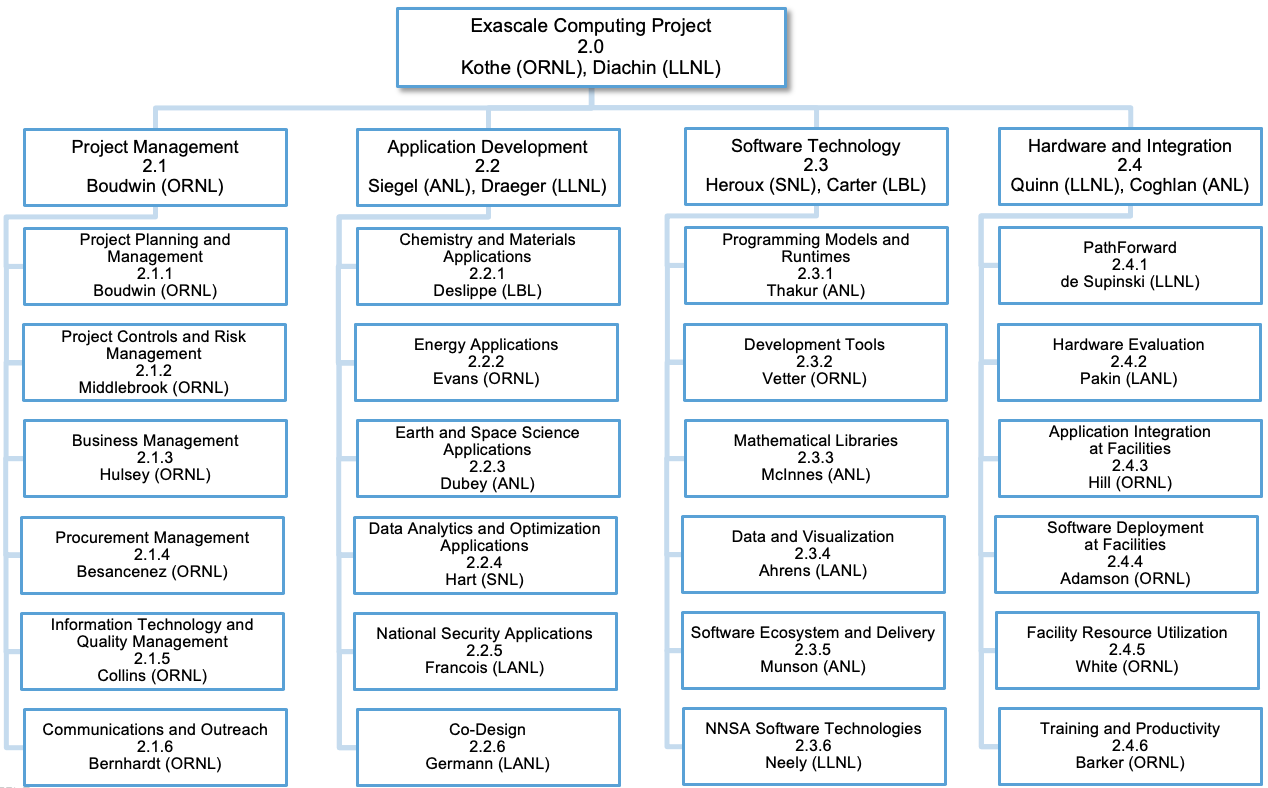
\includegraphics[width=0.9\linewidth]{ECP21}
	\caption{The ECP Work Breakdown Structure through Level 3 (L3) as of December 5, 2019. Under Software Technology, WBS 2.3.6 consolidates ATDM contributions to ECP into a new L3 area.}
	\label{fig:ecp2}
\end{figure}

\subsection{Background}
Historically, the software used on supercomputers has come from three sources: computer system vendors, DOE laboratories, and academia. Traditionally, vendors have supplied system software:  operating system, compilers, runtime, and system-management software. The basic system software is typically augmented by software developed by the DOE HPC facilities to fill gaps or to improve management of the systems. An observation is that it is common for system software to break or not perform well when there is a jump in the scale of the system.
 
Mathematical libraries and tools for supercomputers have traditionally been developed at DOE laboratories and universities and ported to the new computer architectures when they are deployed. These math libraries and tools have been remarkably robust and have supplied some of the most impactful improvements in application performance and productivity. The challenges have been the constant adapting and tuning to rapidly changing architectures.
 
Programming paradigms and the associated programming environments that include compilers, debuggers, message passing, and associated runtimes have traditionally been developed by vendors, DOE laboratories, and universities. The same can be said for file system and storage software. An observation is that the vendor is ultimately responsible for providing a programming environment and file system with the supercomputer, but there is often a struggle to get the vendors to support software developed by others or to invest in new ideas that have few or no users yet. Another observation is that file-system software plays a key role in overall system resilience, and the difficulty of making the file-system software resilient has grown non-linearly with the scale and complexity of the supercomputers.
 
In addition to the lessons learned from traditional approaches, Exascale computers pose unique software challenges including the following.
\begin{itemize}
\item \textbf{Extreme parallelism:} Experience has shown that software breaks at each shift in scale. Exascale systems are predicted to have a billion-way concurrency almost exclusively from discrete accelerator devices, similar to today's GPUs. Because clock speeds have essentially stalled, the 1000-fold increase in potential performance going from Petascale to Exascale is entirely from concurrency improvements.
\item \textbf{Data movement in a deep memory hierarchy: }Data movement has been identified as a key impediment to performance and power consumption. Exascale system designs are increasing the types and layers of memory, which further challenges the software to increase data locality and reuse, while reducing data movement.
\item \textbf{Discrete memory and execution spaces:} The node architectures of Exascale systems include host CPUs and discrete device accelerators.  Programming for these systems requires coordinated transfer of data and work between the host and device. While some of this transfer can be managed implicitly, for the most performance-sensitive phases, the programmer typically must manage host-device coordination explicitly.  Much of the software transformation effort will be focused on this issue.
\end{itemize}
 
In addition to the software challenges imposed by the scale of Exascale computers, the following additional requirements push ECP away from the historical approaches for getting the needed software for DOE supercomputers.
\begin{itemize}
\item \textbf{2021 acceleration:} ECP has a goal of accelerating the development of the U.S. Exascale systems and enabling the first deployment by 2021. This means that the software needs to be ready sooner, and the approach of just waiting until it is ready will not work. A concerted plan that accelerates the development of the highest priority and most impactful software is needed.
\item \textbf{Productivity:} Traditional supercomputer software requires a great deal of expertise to use. ECP has a goal of making Exascale computing accessible to a wider science community than previous supercomputers have been. This requires the development of software that improves productivity and ease of use.
\item \textbf{Diversity:} There is a strong push to make software run across diverse Exascale systems. Accelerator devices from Nvidia have been available for many years and specific host-device programming and execution applications have been successfully ported to these platforms.  Exascale platforms will continue to have this kind of execution model, but with different programming and runtime software stacks.  Writing high-performance, portable code for these platforms will be challenging.
\item \textbf{Analytics and machine learning:} Future DOE supercomputers will need to solve emerging data science and machine learning problems in addition to the traditional modeling and simulation applications. This will require the development of scalable, parallel analytics and machine learning software for scientific applications, much of which does not exist today.
\end{itemize}
 
The next section describes the approach employed by ECP ST to address the Exascale challenges.

\subsection{ECP ST Project Restructuring}\label{subsect:ProjectRestructuring}

The initial organization of ECP ST was based on discussions that occurred over several years of Exascale planning within DOE, especially the DOE Office of Advanced Scientific Computing Research (ASCR).  Figure~\ref{fig:ecpstv1} shows the conceptual diagram of this first phase.  The 66 ECP ST projects were mapped into 8 technical areas, in some cases arbitrating where a project should go based on its primary type of work, even if other work was present in the project.  In November 2017, ECP ST was reorganized into 5 technical areas, primarily through merging a few smaller areas, and the number of projects was reduced to 56 (then 55 due to further merging in \ecosystem).  Figure~\ref{fig:ecpstv2} shows the diagram of the second phase of ECP ST.  In Section~\ref{sect:PETA}, we describe the organization, planning, execution, tracking and assessment processes that will put ECP ST in a good position for success in the CD-2 phase of the project.

\begin{figure}
	\centering
	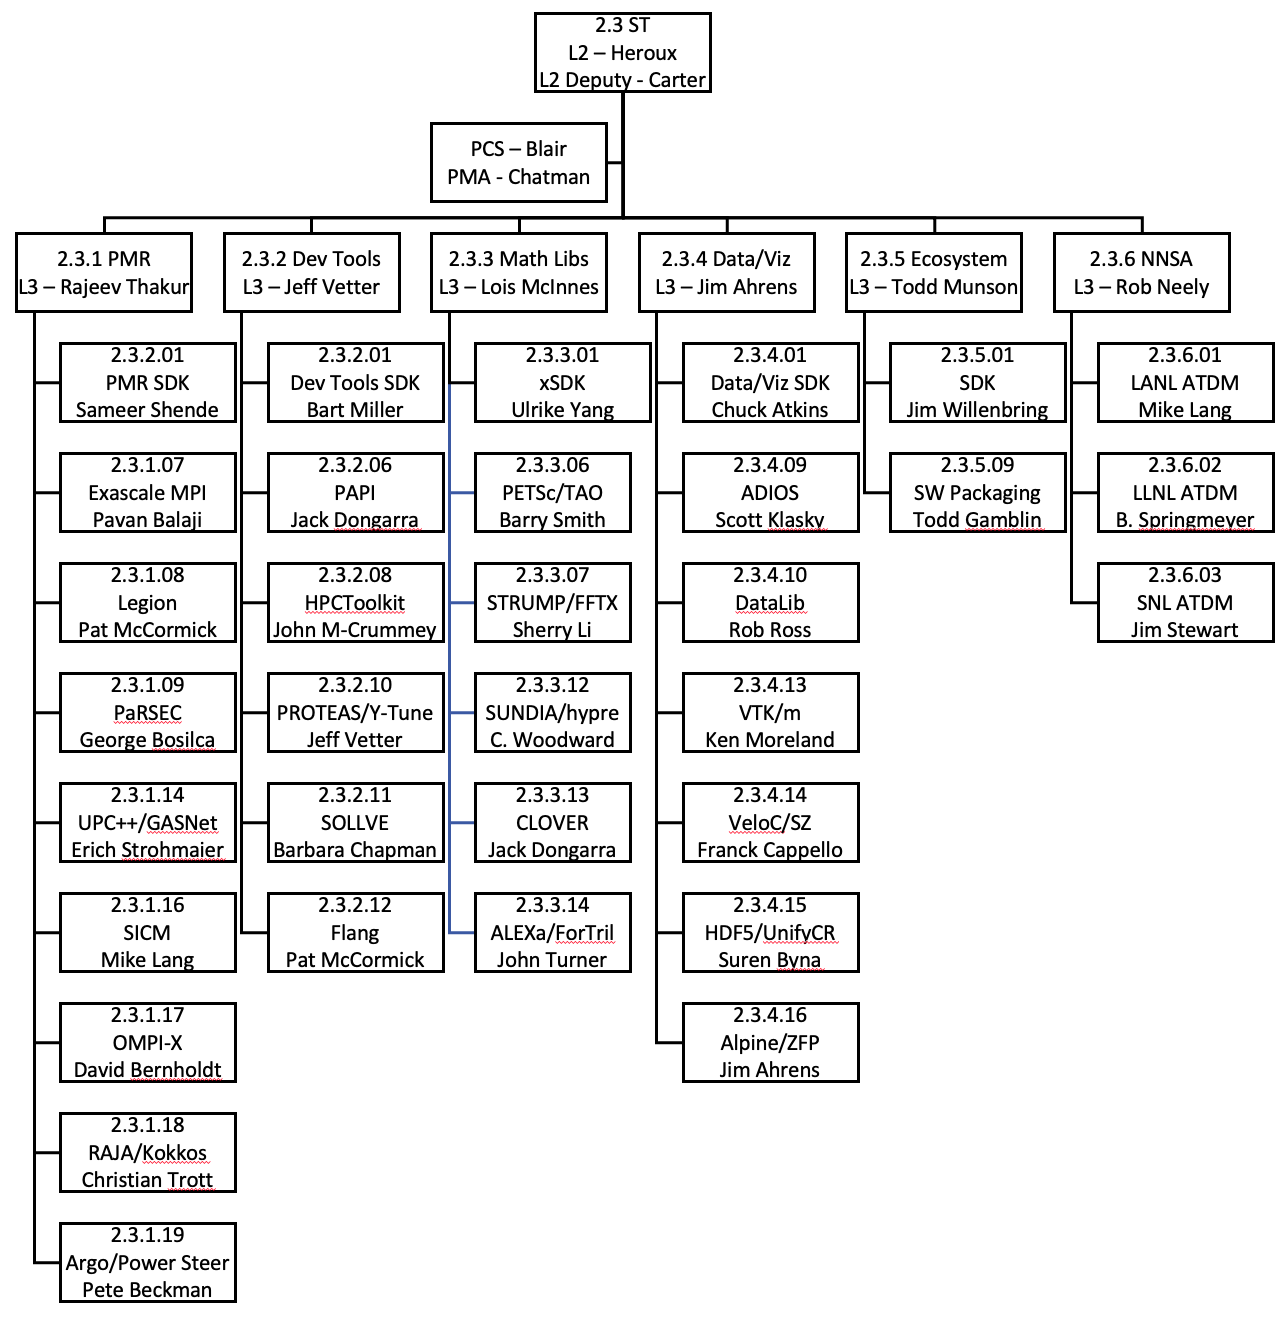
\includegraphics[width=0.9\linewidth]{STFY20WBS}
	\caption{\label{fig:wbs-FY20} The FY20 ECP ST WBS structure as of December 5, 2019, includes a new L3 (2.3.6) and better balances L4 subprojects in the first four L3 technical areas.  Technical area 2.3.5 has only two projects, which are focused on meta-product development in SDKs, E4S, Spack and SuperContainers.}
\end{figure}

\begin{figure}
\begin{mdframed}
\begin{itemize}
\item Phase 1: 66 total L4 subprojects
\begin{itemize}
\item 35 projects funded by the DOE Office of Science that were selected in late 2016 via an RFI and RFP process, considering prioritized requirements of applications and DOE facilities. 
These projects started work in January–March 2017 depending on when the contracts were awarded.
\item 31 ongoing DOE NNSA funded projects that are part of the Advanced Technology Development and Mitigation (ATDM) program. The ATDM program started in FY14.  These projects are focused on longer term research to address the shift in computing technology to extreme, heterogeneous architectures and to advance the capabilities of NNSA simulation codes.
\end{itemize}
\item Phase 2: 55 total L4 subprojects
\begin{itemize}
\item 41 ASCR-funded projects.  Added  2 \ecosystem\ projects and 4 SDK projects.
\item 15 ATDM projects: Combined the previous 31 ATDM projects into one project per technical area per lab.  ATDM projects are generally more vertically integrated and would not perfectly map to any proposed ECP ST technical structure.  Minimizing the number of ATDM projects within the ECP WBS structure reduces complexity of ATDM to ECP coordination and gives ATDM flexibility in revising its portfolio without disruption to the ECP-ATDM mapping.
\end{itemize}
\item Phase 3: 33 total L4 subprojects.  Fewer, larger and more uniform-sized projects
\begin{itemize}
	\item Starting with FY2020, ECP ST has further consolidated L4 projects to foster additional synergies and amortize project overheads as ECP heads into Critical Decision Phase 2~\cite{413.3B}, where more rigor in planning and execution are needed.
	\item 5 L3s to 6: New NNSA ST L3
	\item 40 ST SC-funded L4 subprojects to 30.
	\begin{itemize}
	\item \pmr – 13 to 9, \tools - 6 to 6, \mathlibs - 7 to 6, \dataviz - 10 to 7, \ecosystem - 4 to 3.
	\item Includes 2 new L4 subprojects in SW Ecosystem.
	\end{itemize}
	\item 15 ST NNSA-funded projects transferred to new NNSA ST L3. Consolidated from 15 to 3 L4 subprojects.
	\item No more small subprojects.
	\item Figure~\ref{fig:wbs-FY20} show the overall structure.
\end{itemize}
\end{itemize}
\end{mdframed}

\caption{\label{fig:project-remapping}Project remapping summary from Phase 1 (through November 2017) to Phase 2 (November 2017 -- September 30, 2019) to Phase 3 (After October 1, 2019)}
\end{figure}


\begin{figure}
	\centering
	\includegraphics[width=0.9\linewidth]{ECPSTV1}
	\caption{ECP ST before November 2017 reorganization.  This conceptually layout emerged from several years of Exascale planning, conducted primarily within the DOE Office of Advanced Scientific Computing Research (ASCR).  After a significant restructuring of ECP that removed much of the facilities activities and reduced the project timeline from 10 to seven years, and a growing awareness of what risks had diminished, this diagram no longer represented ECP ST efforts accurately.}
	\label{fig:ecpstv1}
\end{figure}
\begin{figure}
	\centering
	\includegraphics[width=0.9\linewidth]{ECPSTV2}
	\caption{ECP ST after November 2017 reorganization.  This diagram more accurately reflects the priorities and efforts of ECP ST given the new ECP project scope and the demands that we foresee.}
	\label{fig:ecpstv2}
\end{figure}
\begin{figure}
	\centering
	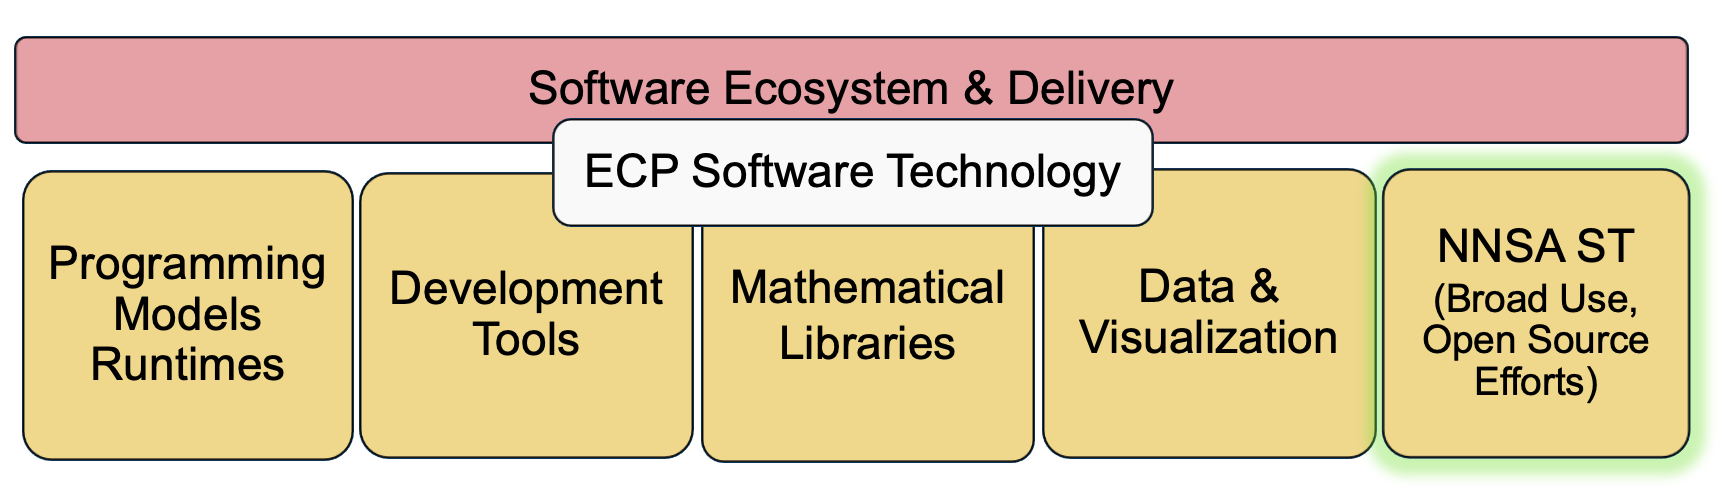
\includegraphics[width=0.9\linewidth]{ECPSTV3}
	\caption{ECP ST after October 2019 reorganization.  This diagram reflects the further consolidation of NNSA open source contributions to enable more flexible management of NNSA ST contributions.}
\end{figure}
\begin{figure}
	\centering
	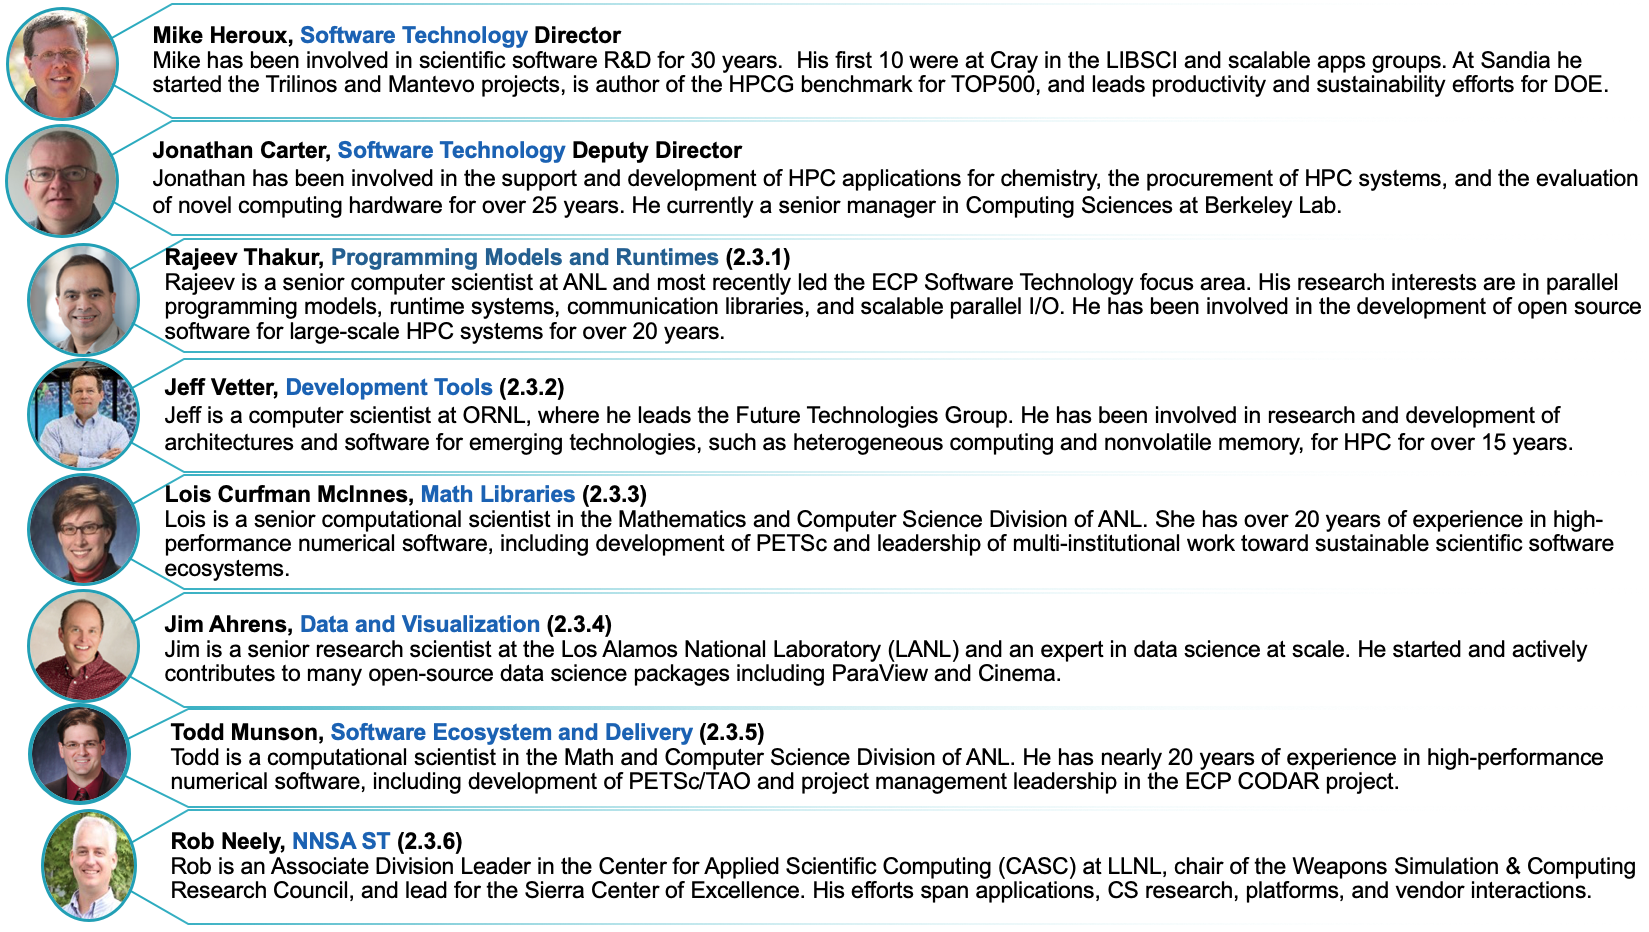
\includegraphics[width=0.9\linewidth]{ECP-ST-Leads}
	\caption{ECP ST Leadership Team as of October 2019.}
	\label{fig:ecpstleads}
\end{figure}



\section{ECP Software Technology Planning, Execution, Tracking and Assessment}\label{sect:PETA}
During the past two years, ECP ST has introduced the Extreme-scale Scientific Software Stack (E4S) and Software Development Kits (SDKs).  We have established new approaches for project planning, execution, tracking and assessment using a tailored earned value management system that enables iterative and incremental refinement to its planning process.  We have also revised our key performance parameter (KPP-3, the third of ECP's four KPPs) to be solely focused on measuring capability integration into client environments.  We have developed and used an assessment process that has led to significant changes in the number and scope of L4 subprojects.

\subsection{ECP Software Technology Architecture and Design}
ECP is taking an approach of codesign across all its principal technical areas: applications development (AD), software technology (ST), and hardware \& integration (HI). For ECP ST, this means its requirements are based on input from other areas, and there is a tight integration of the software products both within the software stack as well as with applications and the evolving hardware. 

The portfolio of projects in ECP ST is intended to address the Exascale challenges and requirements described above. We note that ECP is not developing the entire software stack for an Exascale system. For example, we expect vendors to provide the core software that comes with the system (in many cases, by leveraging ECP and other open-source efforts). Examples of vendor-provided software include operating system, file system, compilers for C, C++, Fortran, etc. (increasingly derived from the LLVM community ecosystem to which ECP contributes), basic math libraries, system monitoring tools, scheduler, debuggers, vendor’s performance tools, MPI (based on ECP-funded projects), OpenMP (with features from ECP-funded project), and data-centric stack components. ECP develops other, mostly higher-level software that is needed by applications and is not vendor specific. ECP-funded software activities are concerned with extreme scalability, exposing additional parallelism, unique requirements of Exascale hardware, and performance-critical components. Other software that aids in developer productivity is needed and may come from third-party open-source efforts.

The ST portfolio includes both ASCR and NNSA ATDM funded efforts. The MOU established between DOE-SC and NNSA has formalized this effort.  Whenever possible, ASCR and ATDM efforts are treated uniformly in ECP ST planning and assessment activities.

ST is also planning to increase integration within the ST portfolio through increased use of software components and application composition vs. monolithic application design. An important transition that ECP can accelerate is the increased development and delivery of reusable scientific software components and libraries. While math and scientific libraries have long been a successful element of the scientific software community, their use can be expanded to include other algorithms and software capabilities, so that applications can be considered more an aggregate composition of reusable components than a monolithic code that uses libraries tangentially.

To accelerate this transition, we need a greater commitment on the part of software component developers to provide reliable and portable software that users can consider to be part of the software ecosystem in much the same way users depend on MPI and compilers. At the same time, we must expect application developers to participate as clients and users of reusable components, using capabilities from components, transitioning away from (or keeping as a backup option) their own custom capabilities.

\subsubsection{The Extreme-scale Scientific Software Stack (E4S)}\label{subsubsect:e4s}
In October 2020, ECP ST released version 1.2 of the Extreme-scale Scientific Software Stack, E4S (\url{http://e4s.io}). E4S contains a collection of the software products to which ECP ST contributes.  E4S is the primary conduit for providing easy access to ECP ST capabilities for ECP and the broader community.  E4S is also the ECP ST vehicle for regression and integration testing across DOE pre-Exascale and Exascale systems.

\begin{figure}
		\centering
		\fbox{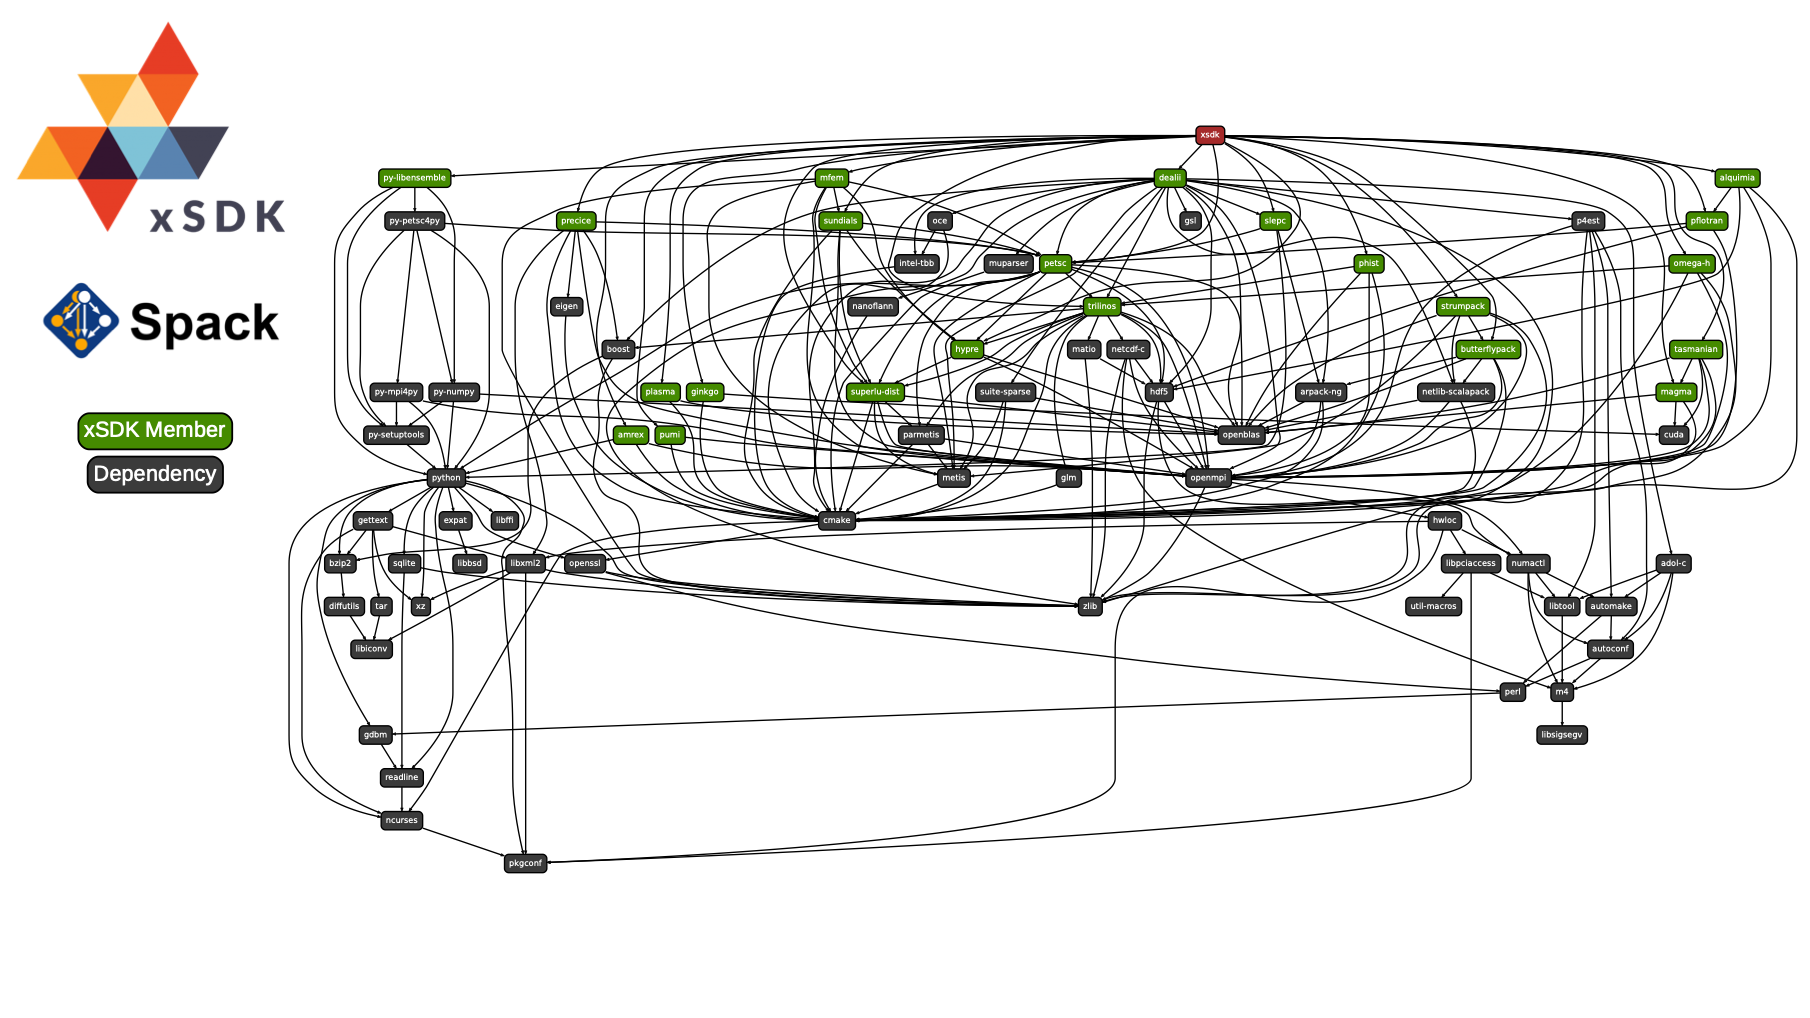
\includegraphics[width=0.9\linewidth]{E4S-Build-Tree}}
	\caption{Using Spack~\cite{gamblin+:ecp18-spack-tutorial}, E4S builds a comprehensive software stack.  As ECP ST efforts proceed, we will use E4S for continuous integration testing, providing developers with rapid feedback on regression errors and providing user facilities with a stable software base as we prepare for Exascale platforms.  This diagram shows how E4S builds ECP products via an SDK target (the math libraries SDK called xSDK in this example).  The SDK target then builds all product that are part of the SDK (see Figure~\ref{fig:sdk-definition1} for SDK groupings), first defining and building external software products. Green-labeled products are part of the SDK. The blue-label indicates expected system tools, in this case a particular version of Python.  Black-labeled products are expected to be previously installed into the environment (a common requirement and easily satisfied).  Using this approach, a user who is interested in only SUNDIALS (a particular math library) can be assured that the SUNDIALS build will be possible since it is a portion of what E4S builds and tests.}
	\label{fig:e4s-build-tree}
\end{figure}

E4S has the following key features:
\begin{itemize}
	\item \textbf{The E4S suite is a large and growing effort to build and test a comprehensive scientific software ecosystem:} In November 2018, E4S V0.1 contained 25 ECP products.  Two years later, E4S V1.2, the fifth E4S release, contained 67 ECP ST products and numerous additional products needed for a complete software environment.  Eventually E4S will contain all open source products to which ECP contributes, and all related products needed for a holistic environment.
	\item \textbf{E4S is not an ECP-specific software suite:}  The products in E4S represent a holistic collection of capabilities that contain the ever-growing SDK collections sponsored by ECP and all additional underlying software required to use ECP ST capabilities.  Furthermore, we expect the E4S effort to live beyond the timespan of ECP, becoming a critical element of the scientific software ecosystem.
	\item \textbf{E4S is partitionable:} E4S products are built and tested together using a tree-based hierarchical build process.  Because we build and test the entire E4S tree, users can build any subtree of interest, without building the whole stack (see Figure~\ref{fig:e4s-build-tree}).
	\item \textbf{E4S uses Spack:} The Spack~\cite{gamblin+:ecp18-spack-tutorial} meta-build tool invokes the native build process of each product, enabling quick integration of new products, including non-ECP products.
	\item \textbf{E4S is available via containers:} In addition to a build-from-source capability using Spack, E4S maintains several container environments (Docker, Singularity, Shifter, CharlieCloud) that provides the lowest barrier to use.  Container distributions dramatically reduce installation costs and provide a ready-made environment for tutorials that leverage E4S capabilities.  For example, E4S containers now support custom images for ECP applications such as WDMapp and Pantheon.
	\item \textbf{E4S distribution:} E4S products are available at \url{http://e4s.io}.
	\item \textbf{E4S developer community resources:} Developers interested in participating in E4S can visit the E4S-Project GitHub community at \url{https://github.com/E4S-Project}.	
\end{itemize}

\begin{figure}
	\centering
	\fbox{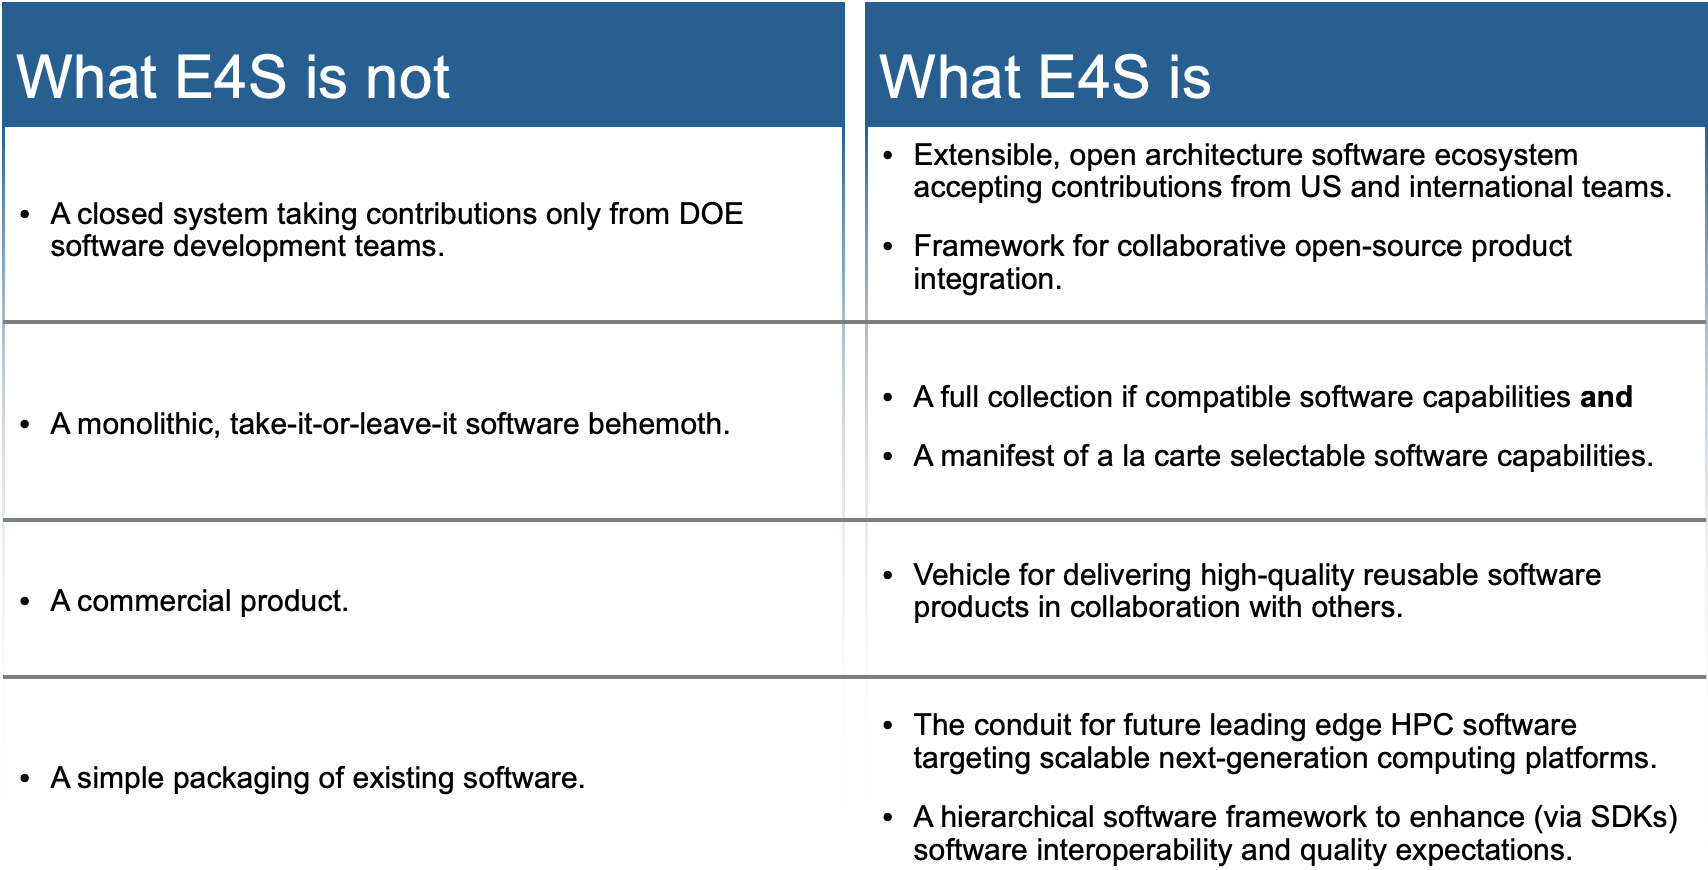
\includegraphics[width=0.9\linewidth]{E4S-Summary}}
	\caption{The Extreme-scale Scientific Software Stack (E4S) provides a complete Linux-based software stack that is suitable for many scientific workloads, tutorial and development environments.  At the same time, it is an open software architecture that can expand to include any additional and compatible Spack-enabled software capabilities. Since Spack packages are available for many products and easily created for others, E4S is practically expandable to include almost any robust Linux-based product.  Furthermore, E4S capabilities are available as subtrees of the full build: E4S is not monolithic.}
	\label{fig:e4s-is-isnot}
\end{figure}

\begin{figure}
	\centering
	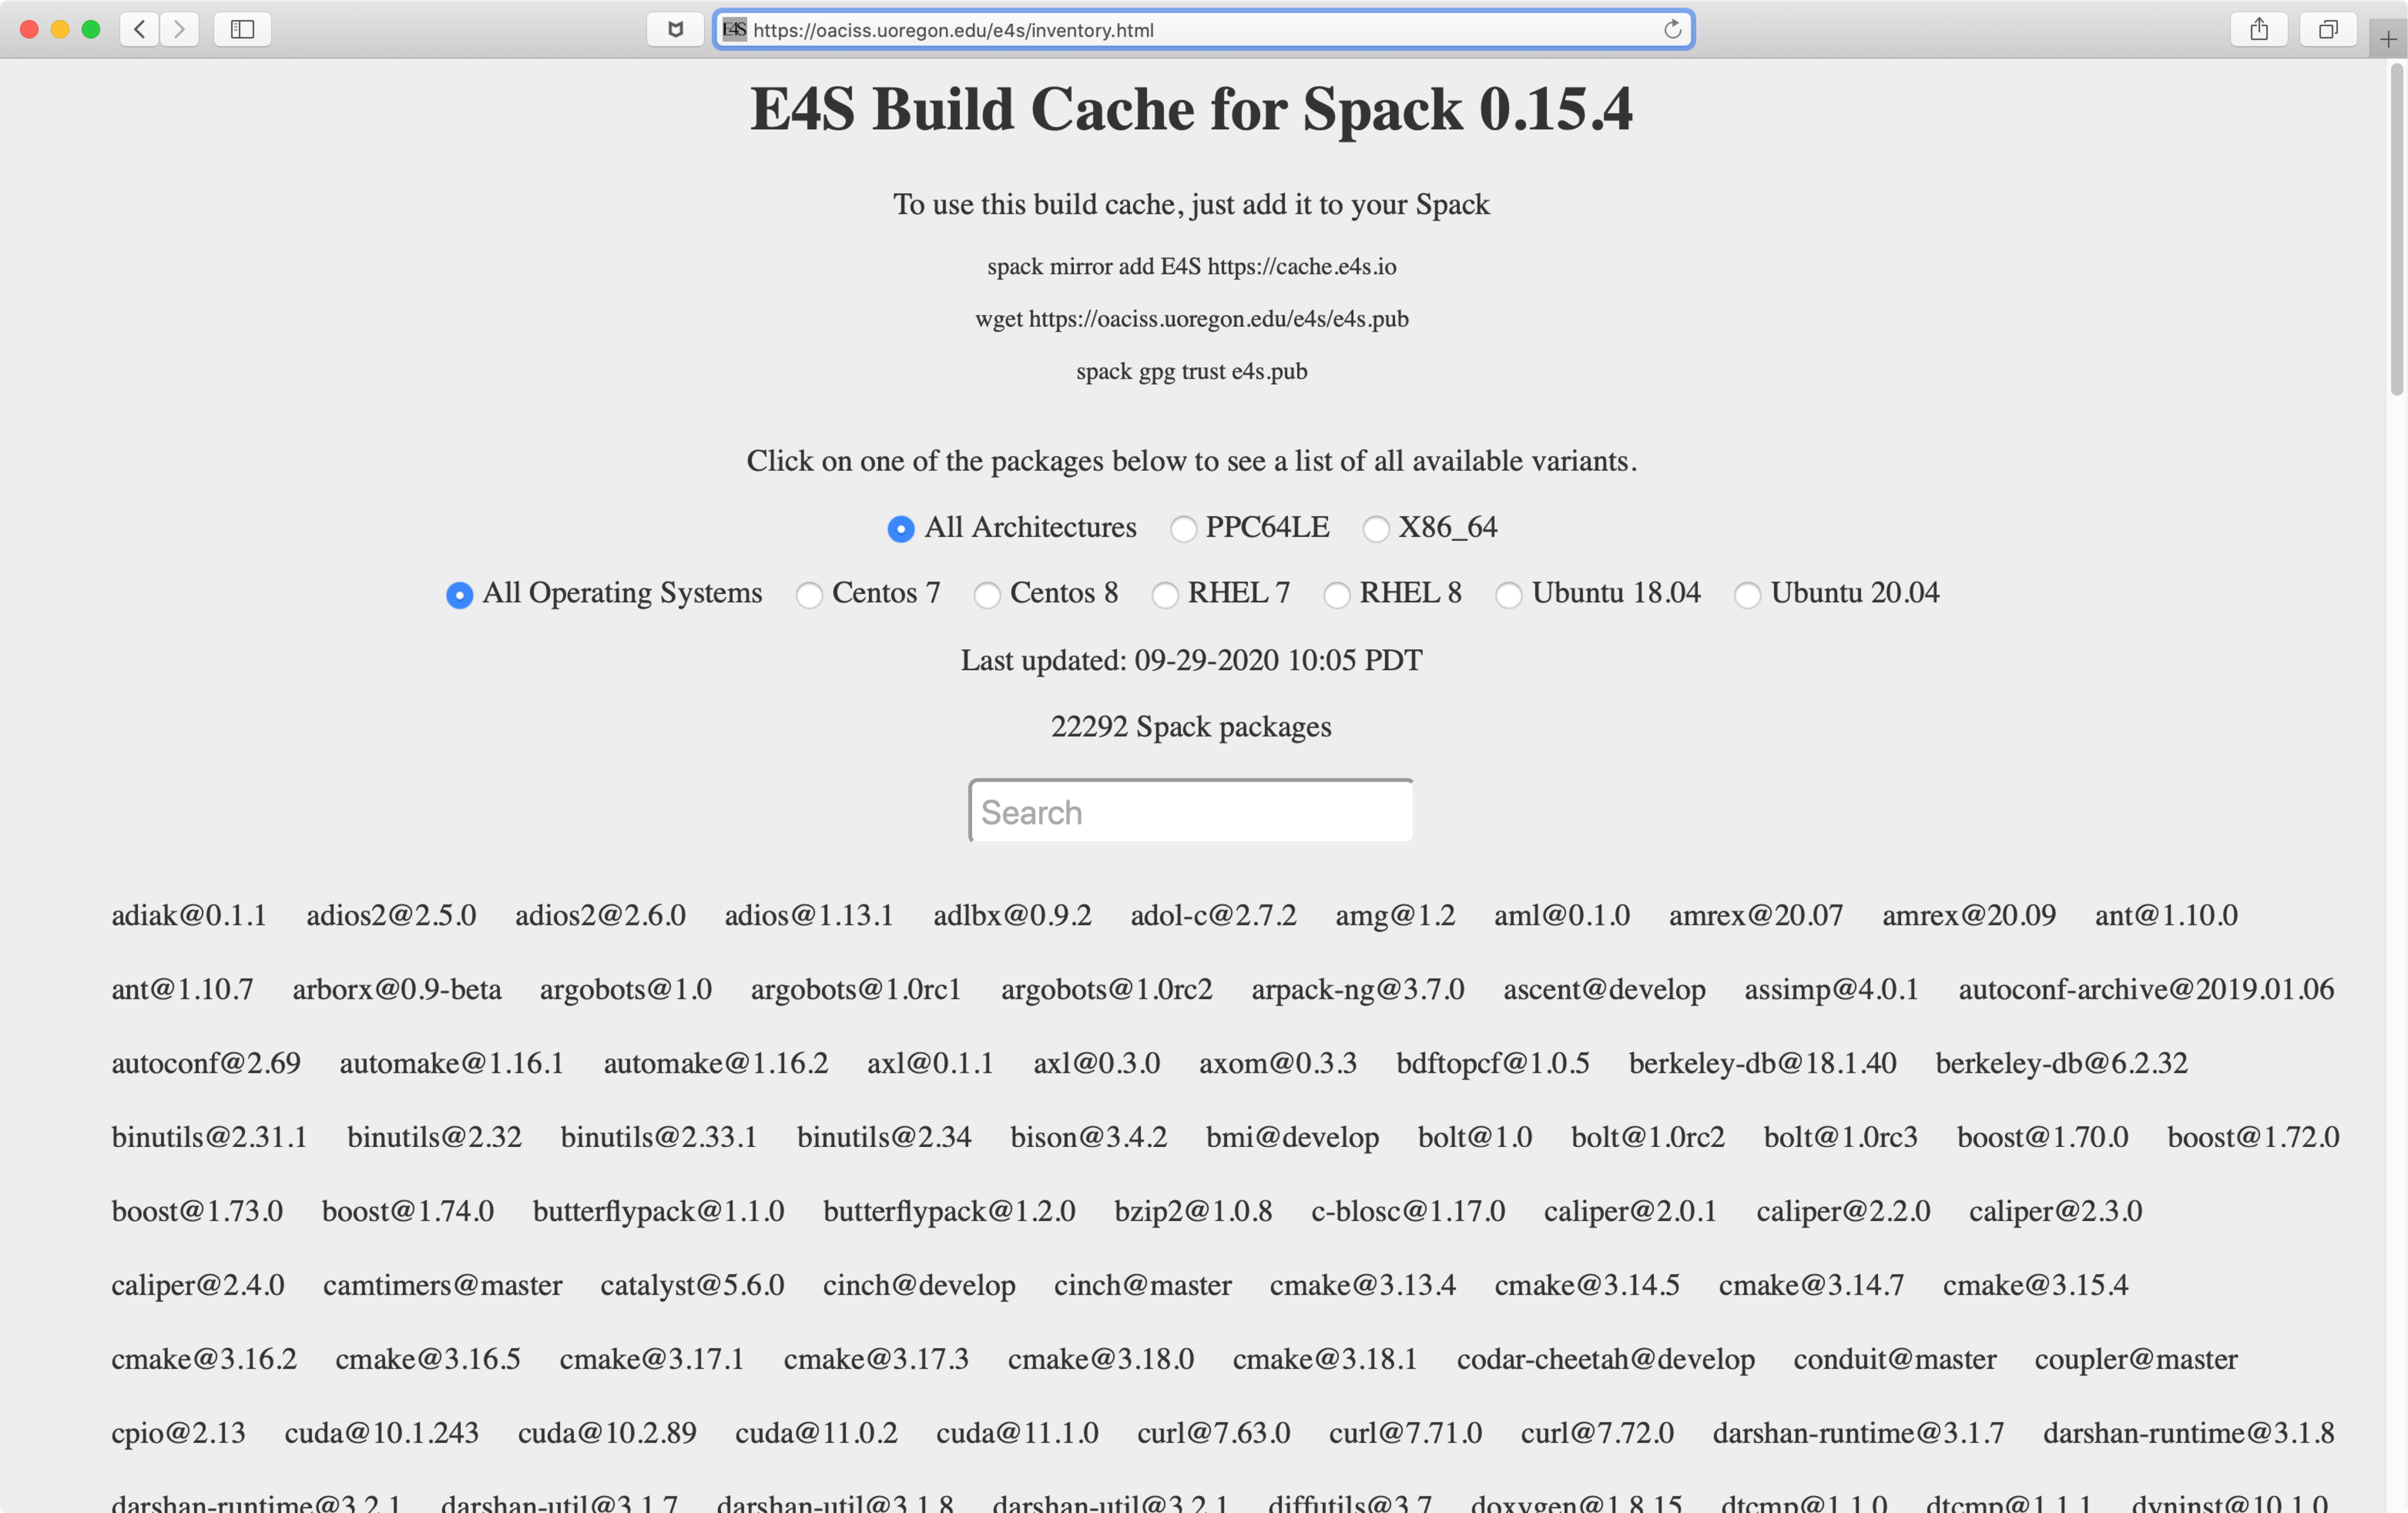
\includegraphics[width=0.9\linewidth]{E4S-Build-Cache-Binaries-2020}
	\caption{Using Spack build cache features, E4S builds can be accelerated by use of cached binaries for any build signature that Spack has already seen. Between September 2019 and September 2020, more than 21,000 binaries were added to the cache.}
	\label{fig:e4s-build-cache}
\end{figure}

\begin{figure}
	\centering
	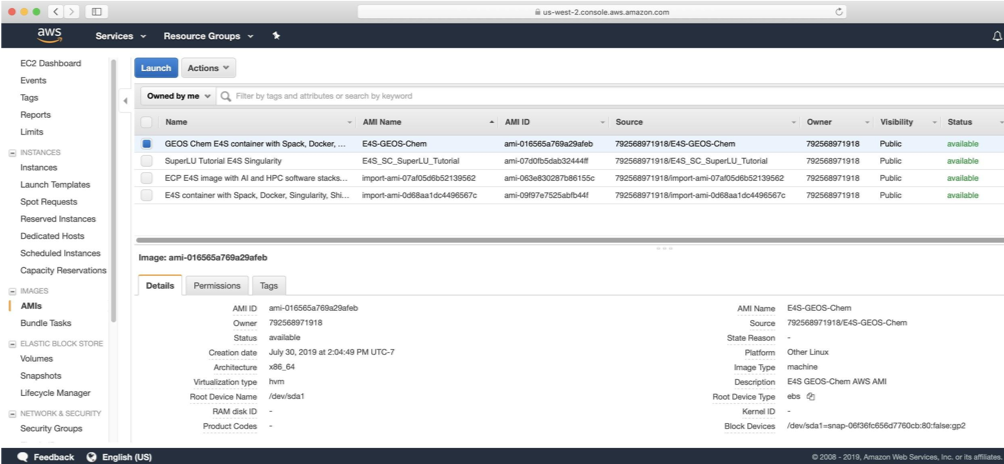
\includegraphics[width=0.9\linewidth]{E4S-AWS-public-image}
	\caption{E4S is available as an Amazon AWS public image.  Images on Google and Microsoft Cloud environments will be available soon.}
	\label{fig:e4s-aws-image}
\end{figure}


The E4S effort is described in further detail in Sections~\ref{subsect:ecosystem}, especially Section~\ref{subsubsect:sdks}.

\subsubsection{Software Development Kits}\label{subsubsect:sdks}
One opportunity for a large software ecosystem project such as ECP ST is to foster increased collaboration, integration and interoperability among its funded efforts. Part of ECP ST design is the creation of software development kits (SDKs).  SDKs are collections of related software products (called packages) where coordination across package teams will improve usability and practices and foster community growth among teams that develop similar and complementary capabilities. SDKs have the following attributes:
\begin{table}
	\begin{mdframed}
\begin{enumerate}
	\item \textbf{Domain scope:} Each SDK will be composed of packages whose capabilities are within a natural functionality domain. Packages within an SDK provide similar capabilities that can enable leveraging of common requirements, design, testing and similar activities. Packages may have a tight complementary such that ready composability is valuable to the user.
	\item \textbf{Interaction models:} How packages within an SDK interact with each other. Interactions include common data infrastructure, or seamless integration of other data infrastructures; access to capabilities from one package for use in another.
	\item \textbf{Community policies:} Expectations for how package teams will conduct activities, the services they provide, software standards they follow, and other practices that can be commonly expected from a package in the SDK.
	\item \textbf{Meta-build system:} Robust tools and processes to build (from source), install and test the SDK with compatible versions of each package. This system sits on top of the existing build, install and test capabilities for each package.
	\item \textbf{Coordinated plans:} Development plans for each package will include efforts to improve SDK capabilities and lead to better integration and interoperability.
	\item \textbf{Community outreach:} Efforts to reach out to the user and client communities will include explicit focus on SDK as product suite.
\end{enumerate}
	\end{mdframed}
\caption{\label{table:sdk-attributes} Software Development Kits (SDKs) provide an aggregation of software products that have complementary or similar attributes.  ECP ST uses SDKs to better assure product interoperability and compatibility.  SDKs are also essential aggregation points for coordinated planning and testing. SDKs are an integral element of ECP ST~\cite{Heroux-SDK-Podcast}.  Section~\ref{subsubsect:ecosystem-sdk} describes the six SDK groupings and the current status of the SDK effort.}
\end{table}

\paragraph{ECP ST SDKs}
As part of the delivery of ECP ST capabilities, we will establish and grow a collection of SDKs. The new layer of aggregation that SDKs represent are important for improving all aspects of product development and delivery. The communities that will emerge from SDK efforts will lead to better collaboration and higher quality products. Established community policies will provide a means to grow SDKs beyond ECP to include any relevant external effort. The meta-build systems (based on Spack) will play an important role in managing the complexity of building the ECP ST software stack, by providing a new layer where versioning, consistency and build options management can be addressed at a mid-scope, below the global build of ECP ST products.
Each ECP ST L3 (five of them) has funds for an SDK project from which we have identified a total of six SDKs and an at-large collection of remaining products that will be delivered outside of the SDK grouping.  Section~\ref{subsubsect:ecosystem-sdk} provides an update on the progress in defining SDK groupings. For visibility, we provide the same diagram in Figure~\ref{fig:sdk-definition1-0}.

\begin{figure}[htb]
	\centering
	\fbox{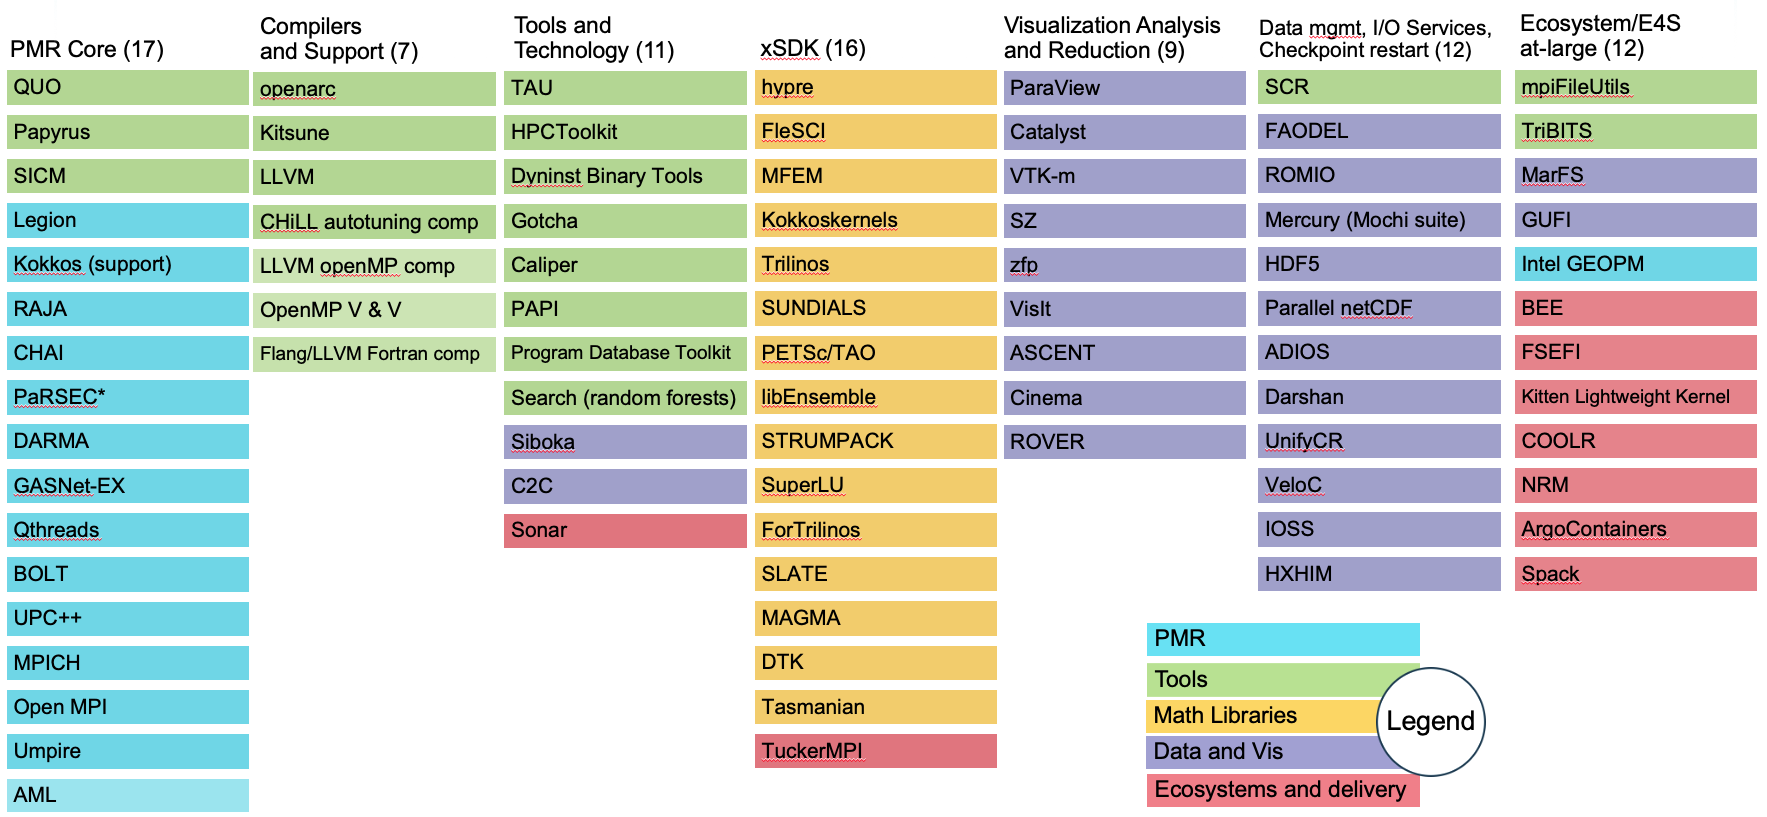
\includegraphics[width=6.5in]{projects/2.3.5-Ecosystem/2.3.5.01-Ecosystem-SDK/SDKdefinition2}}
	\caption{\label{fig:sdk-definition1-0}The above graphic shows the breakdown of ECP ST products into 6 SDKs ( the first six columns).  The rightmost column lists products that are not part of an SDK, but are part of Ecosystem group that will also be delivered as part of E4S. The colors denoted in the key map all of the ST products to the ST technical area they are part of.  For example, the xSDK consists of products that are in the Math Libraries Technical area, plus TuckerMPI which is in the Ecosystem and Delivery technical area.  Section~\ref{subsubsect:ecosystem-sdk} provides an update on the progress in defining SDK groupings.}
\end{figure}


\subsubsection{ECP ST Product Dictionary}\label{subsubsect:dictionary}
In the past year, ECP has initiated an effort to explicitly manage ECP ST products and their dependencies (see Section~\ref{subsubsect:dep-management}).  In order to eliminate ambiguities, we first need a product dictionary: an official list of publicly-name products to which ECP ST teams contribute their capabilities and upon which ECP ST clients depend.  The ECP Product Dictionary is single, managed table.  It presently contains 70 primary products along with subproducts that are either components within a product or particular implementations if a standard API.  Two special primary products are the Facilities stack and Vendor stack.  Having these stacks on the list enables ST teams to indicate that their capabilities are being delivered to ecosystems outside of ECP.

Figure~\ref{fig:product-dictionary-overview} describes the policy for ECP ST teams to add and manage their contributions to the Product Dictionary.  Figure~\ref{fig:product-dictionary} shows a snapshot of the beginning and end of the current ECP ST Product Dictionary, which is maintained on the ECP Confluence wiki.

\begin{figure}
	\centering
	\fbox{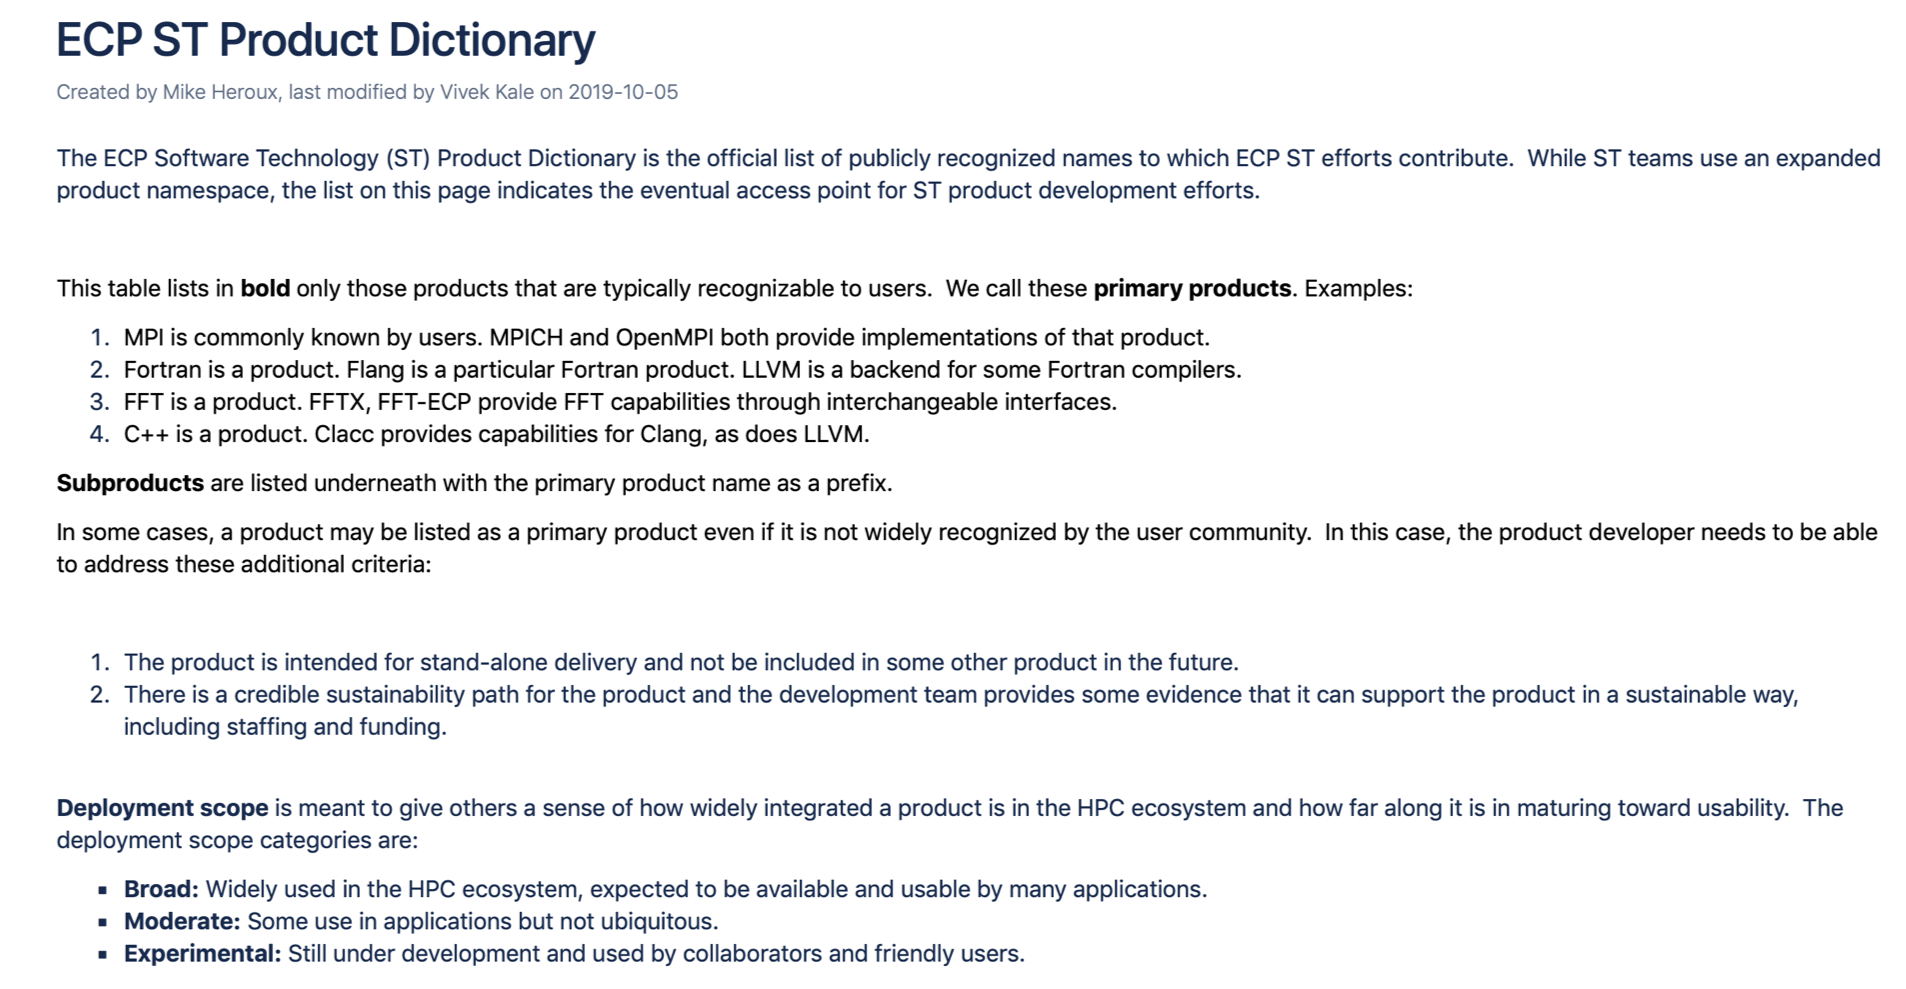
\includegraphics[width=0.9\linewidth]{ProductDictionaryOverview}}
	\caption{This figure shows a screenshot from the top of the ECP Confluence wiki page containing the ECP ST Product Dictionary.  The Product Dictionary structure contains primary and secondary products.  Client (consumer) dependencies are stated against the primary product names only, enabling unambiguous mapping of AD-on-ST and ST-on-ST dependencies.}
	\label{fig:product-dictionary-overview}
\end{figure}

\begin{figure}
	\centering
	\fbox{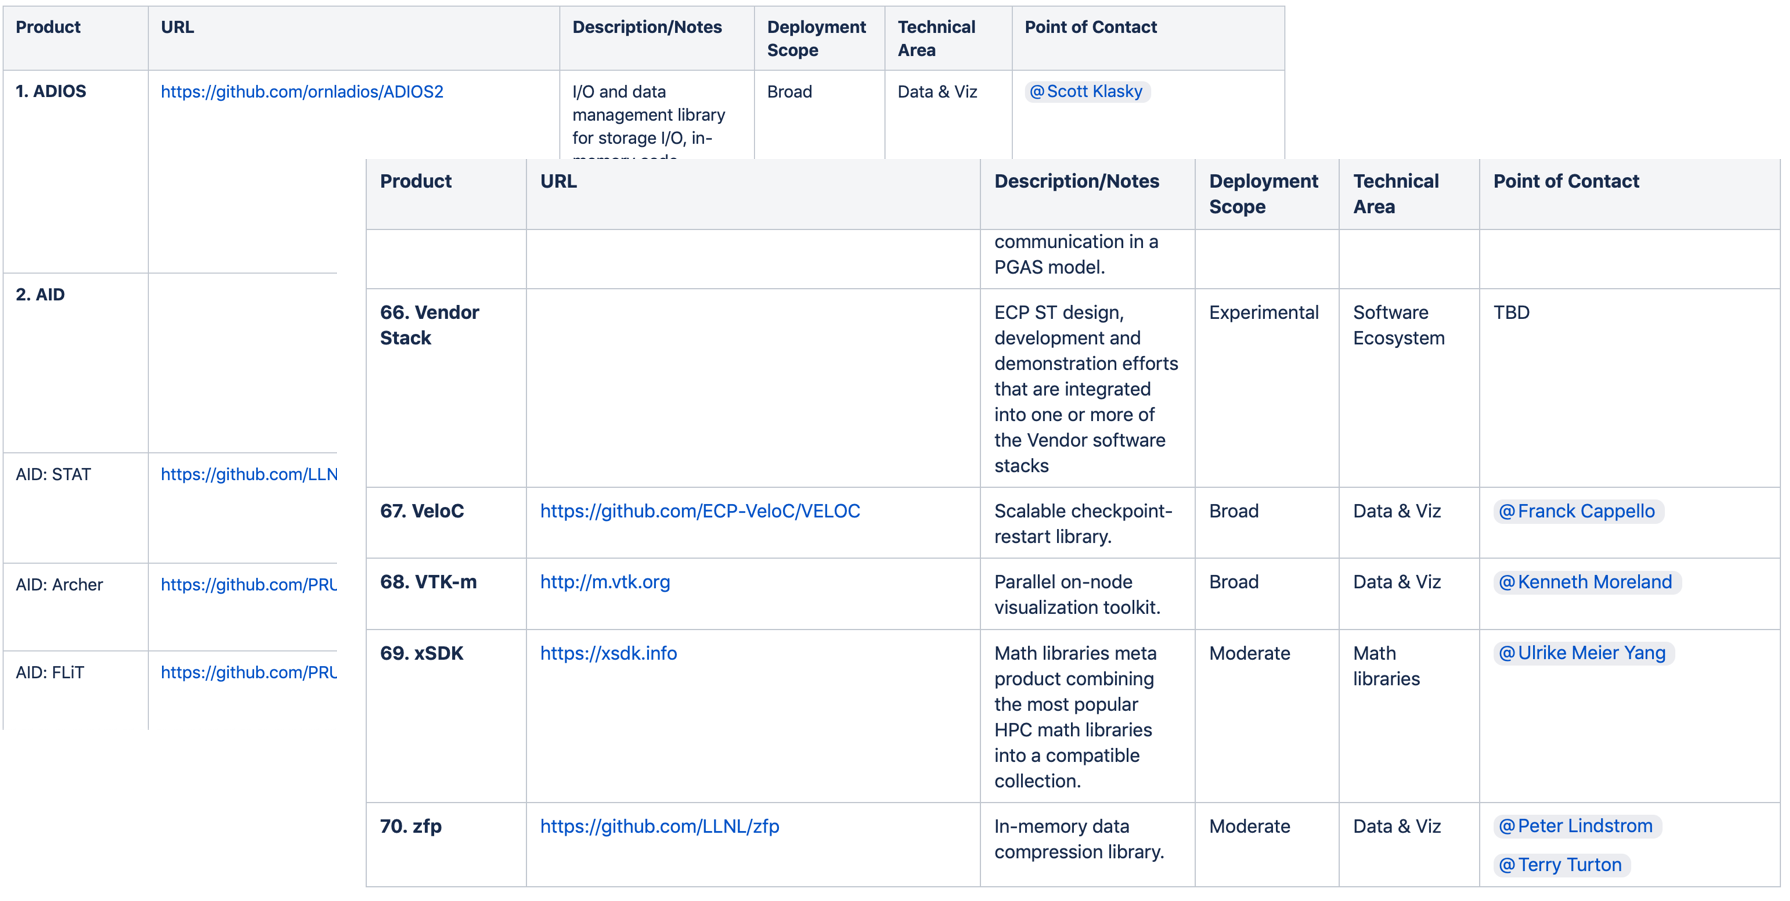
\includegraphics[width=0.9\linewidth]{ConfluenceProductDictionaryExample}}
	\caption{These screen shots are from the ECP Confluence Product Dictionary Table.  The table is actively managed to include primary and secondary products to which ECP ST team contribute and upon which ECP ST clients depend.  Presently the Product Dictionary contains 70 primary products.  Secondary products are listed under the primary product with the primary product as a prefix.  For example, AID is the second listed primary product in this figure.  STAT, Archer and FLIT are component subproducts.  MPI (not shown) is another primary product.  MPICH and OpenMPI are two robust MPI implementations and are listed as MPI subproducts.}
	\label{fig:product-dictionary}
\end{figure}

\subsubsection{ECP Product Dependency Management}\label{subsubsect:dep-management}
Given the ECP ST Product Dictionary, and a similar dictionary for ECP AD and Co-Design products, ECP as a project has created a dependency database that enabled creation and characterization of product-to-product dependencies.  ECP manages these dependencies in a Jira database using a custom Jira issue type, Dependency.  The dependency database provides an important tool for understanding and managing ECP activities.  The dependency information is valuable both within and outside the project.  Figure

\begin{figure}
	\centering
	\fbox{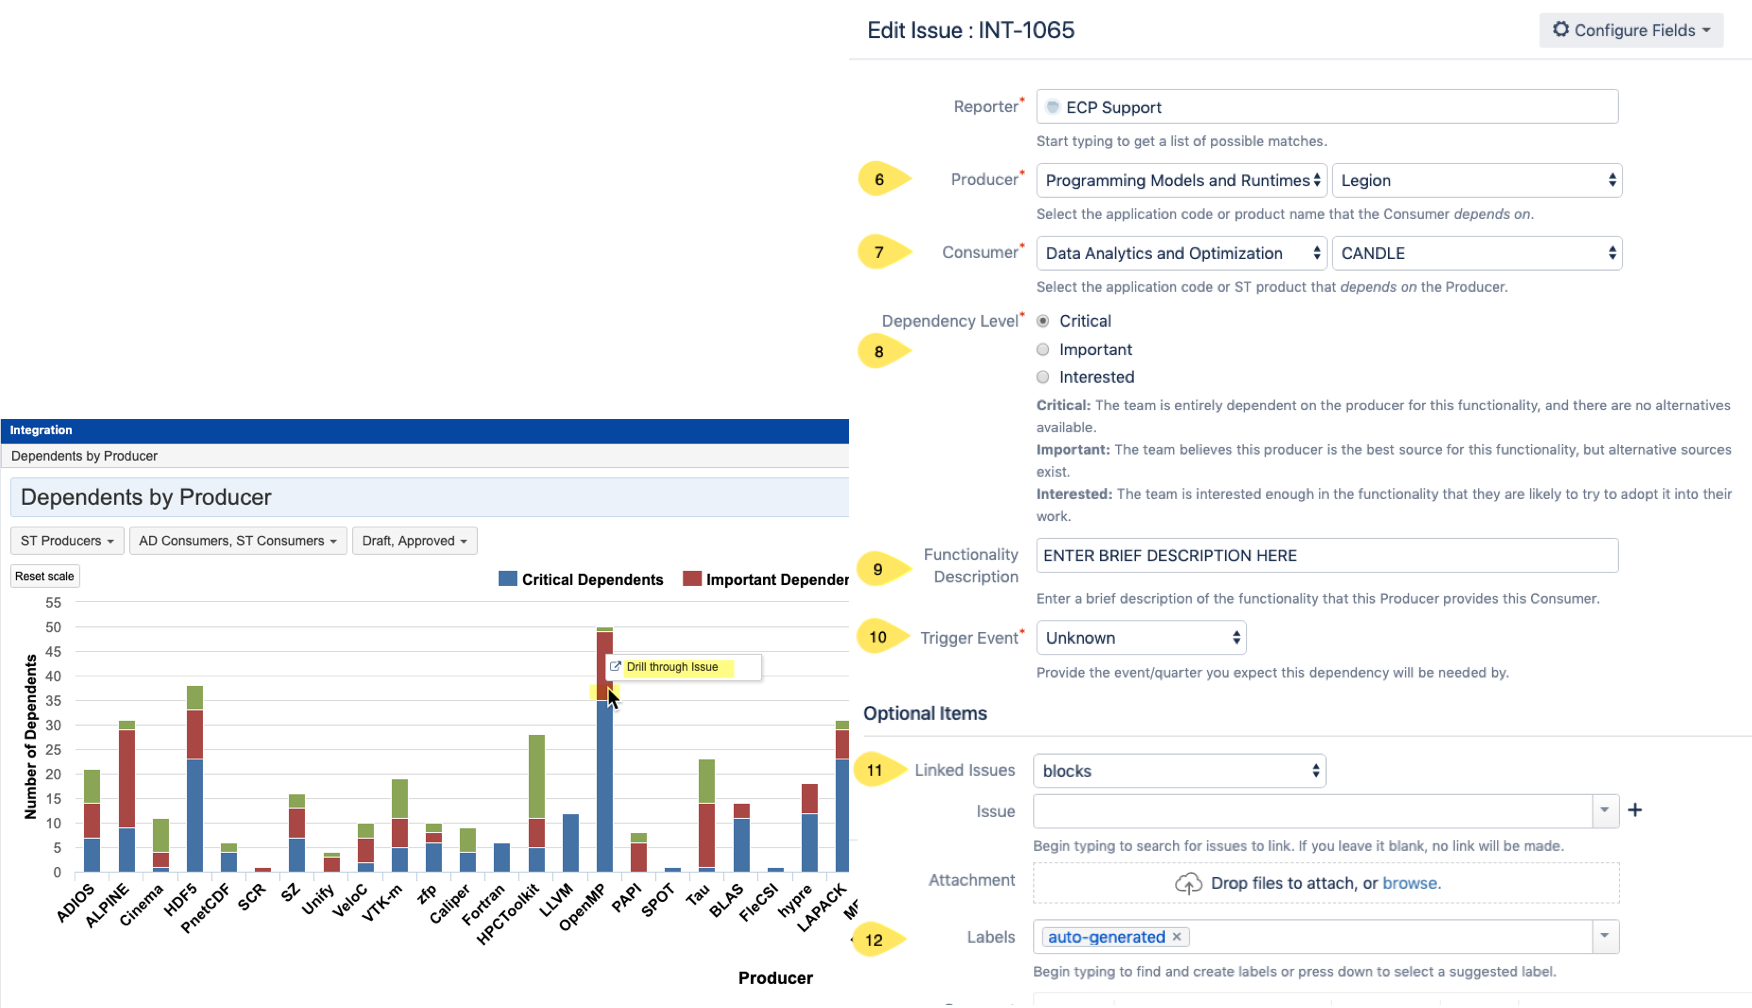
\includegraphics[width=0.9\linewidth]{DependencyDashboard-EditPanel}}
	\caption{Using Jira, ECP manages its AD, ST, HI, vendor and facilities dependencies.  This figure shows a dashboard snapshot along with an edit panel that support creation and management of a consumer-on-producer dependency.}
	\label{fig:dependency-dashboard-edit}
\end{figure}

\begin{figure}
	\centering
	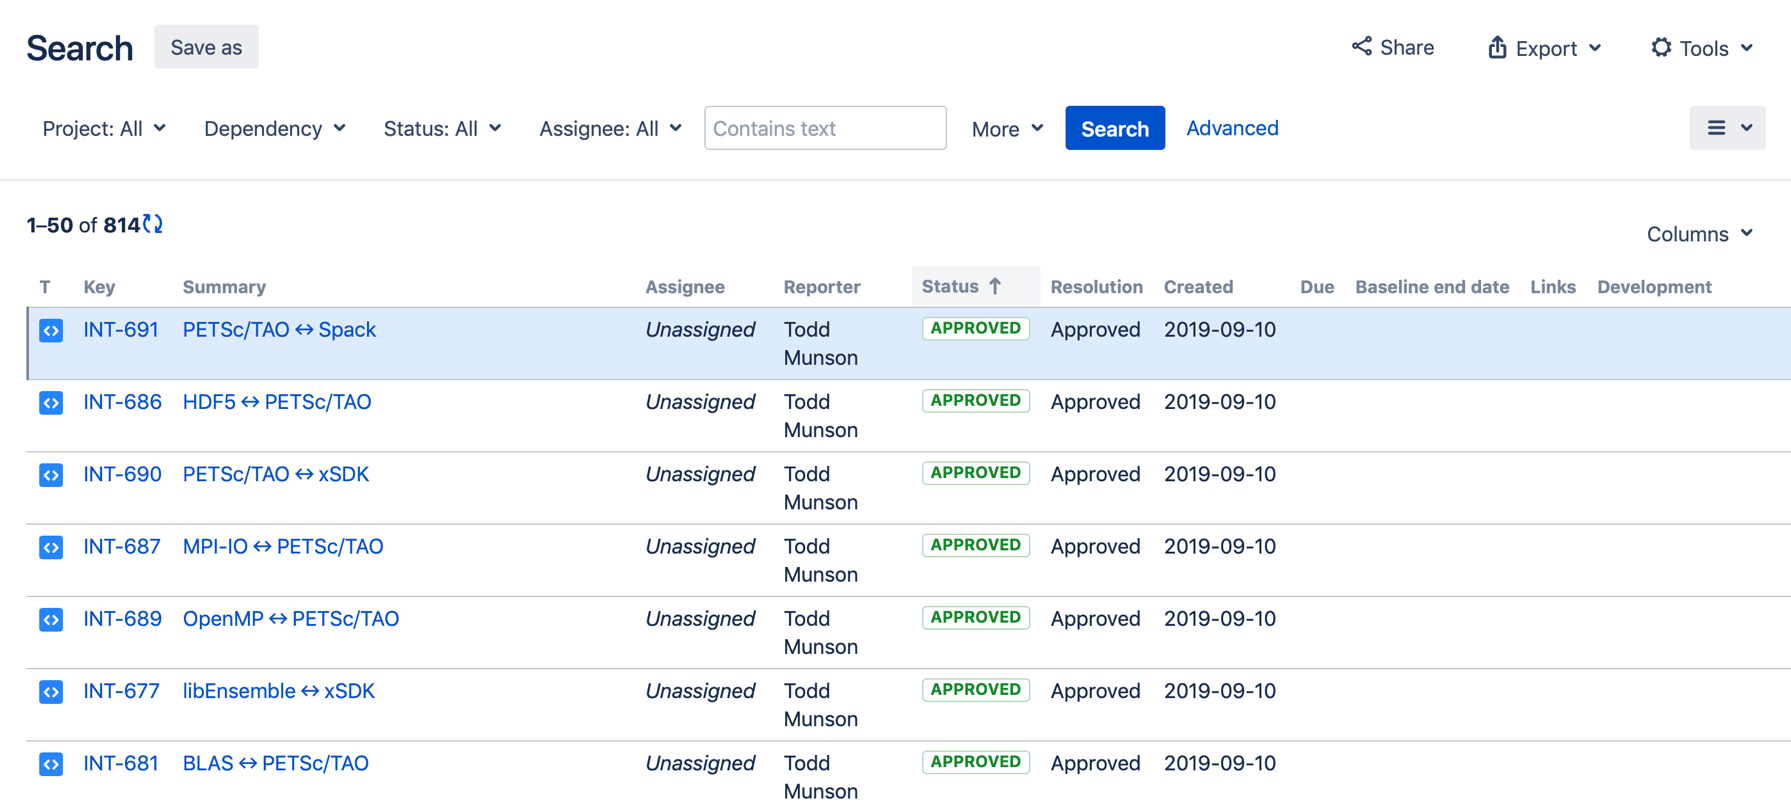
\includegraphics[width=0.9\linewidth]{PETSc-TAO-Dependencies}
	\caption{This query result from the ECP Jira Dependency database lists all consumers of capabilities from the PETSc/TAO product.  By selecting the details of one of the dependency issues, one can further see how critical the dependency is and see any custom information peculiar to the particular dependency.}
	\label{fig:petsc-tao-dependencies}
\end{figure}

\newpage
\subsection{ECP ST Planning and Tracking}

While ECP is an official 413.3b federal construction project using an earned value management (EVM) structure, we are permitted to tailor the planning process in order to obtain the flexibility needed for a software project whose requirements are emerging as the project proceeds.  In this section, we describe how ECP ST plans it activities using the Jira project management tool.  We first discuss P6 Activities (similar to milestones) and then discuss the key performance parameter (KPP-3) associated with ECP ST.


\subsubsection{ECP ST P6 Activity Issues}

ECP ST uses a custom Jira issue type called P6 Activity.  Each L4 subproject creates a series of P6 Activity issues extending to the end of ECP (Q3FY23).  Except for the current fiscal year, a single P6 Activity issue describes expected deliverables as a planning package.  Six months prior to the start of a fiscal year, the planning package for the coming year is replaced with 4--6 issues spanning the year with baseline start and end dates, an estimate of the percent annual budget and a high level description.  Eight weeks prior to the start of an activity, full details about staffing, completion criteria and more are added to the issue.  Figure~\ref{fig:planning-process} show the steps in diagram form.  

Cost, scope and schedule for ECP ST is tracked and managed by monitoring progress of the collection of P6 Activities.  Value is accrued when a P6 Activity issue is marked Done in the Jira database.  Schedule and cost performance indices are derived from the status of our P6 Activities.  Schedule, cost and scope changes against the plan are managed via a formal project change request (PCR) process.

\begin{figure}
	\centering
	\fbox{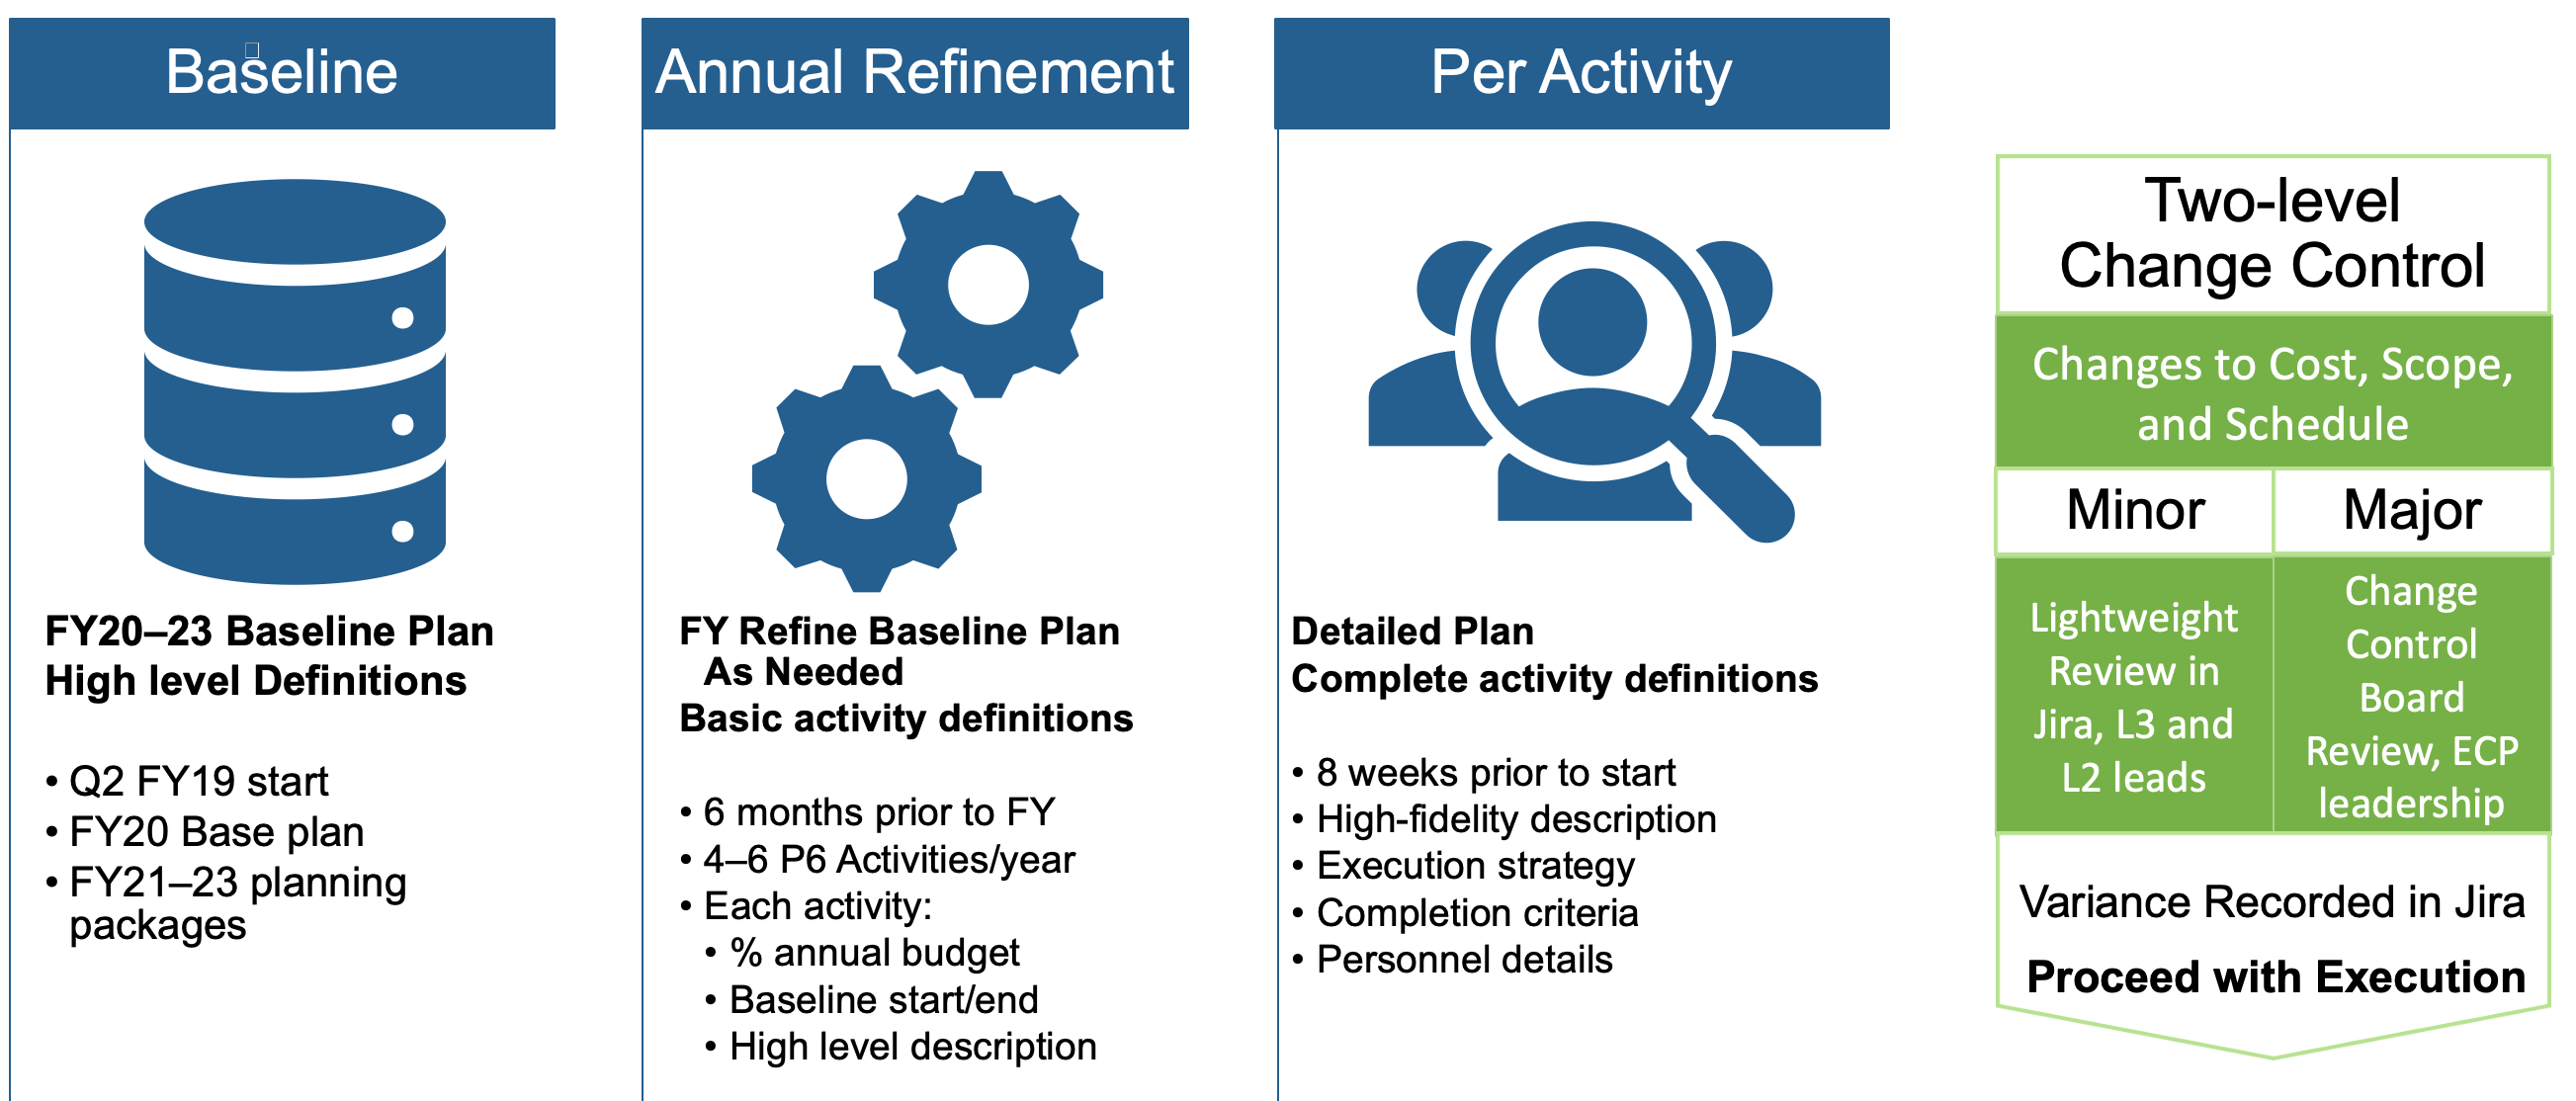
\includegraphics[width=0.9\linewidth]{Planning-Process}}
	\caption{ECP ST uses a custom Jira issue type called P6 Activity.  Each L4 subproject creates a series of these issues extending to the end of ECP.  Except for the current fiscal year, a single P6 Activity issue describes expected deliverables as a planning package.  Six months prior to the start of a fiscal year, the planning package is replaced with 4--6 issues spanning the coming year.  Eight weeks prior to the start of an activity, full details about staffing, completion criteria and more are added to the issue.}
	\label{fig:planning-process}
\end{figure}


\subsubsection{Key Performance Parameter (KPP) 3}

ECP has four Key Performance Parameters (KPPs).  Figure~\ref{fig:kpp-definitions} shows the KPP definitions. KPP-3 is focused on a productive and sustainable software ecosystem. ECP ST is the primary owner of this KPP (along with co-design projects in ECP AD).  The focus of KPP-3 is defining and tracking capability integrations of ST products into client environment, as described in this section. 

\begin{figure}
	\centering
	\fbox{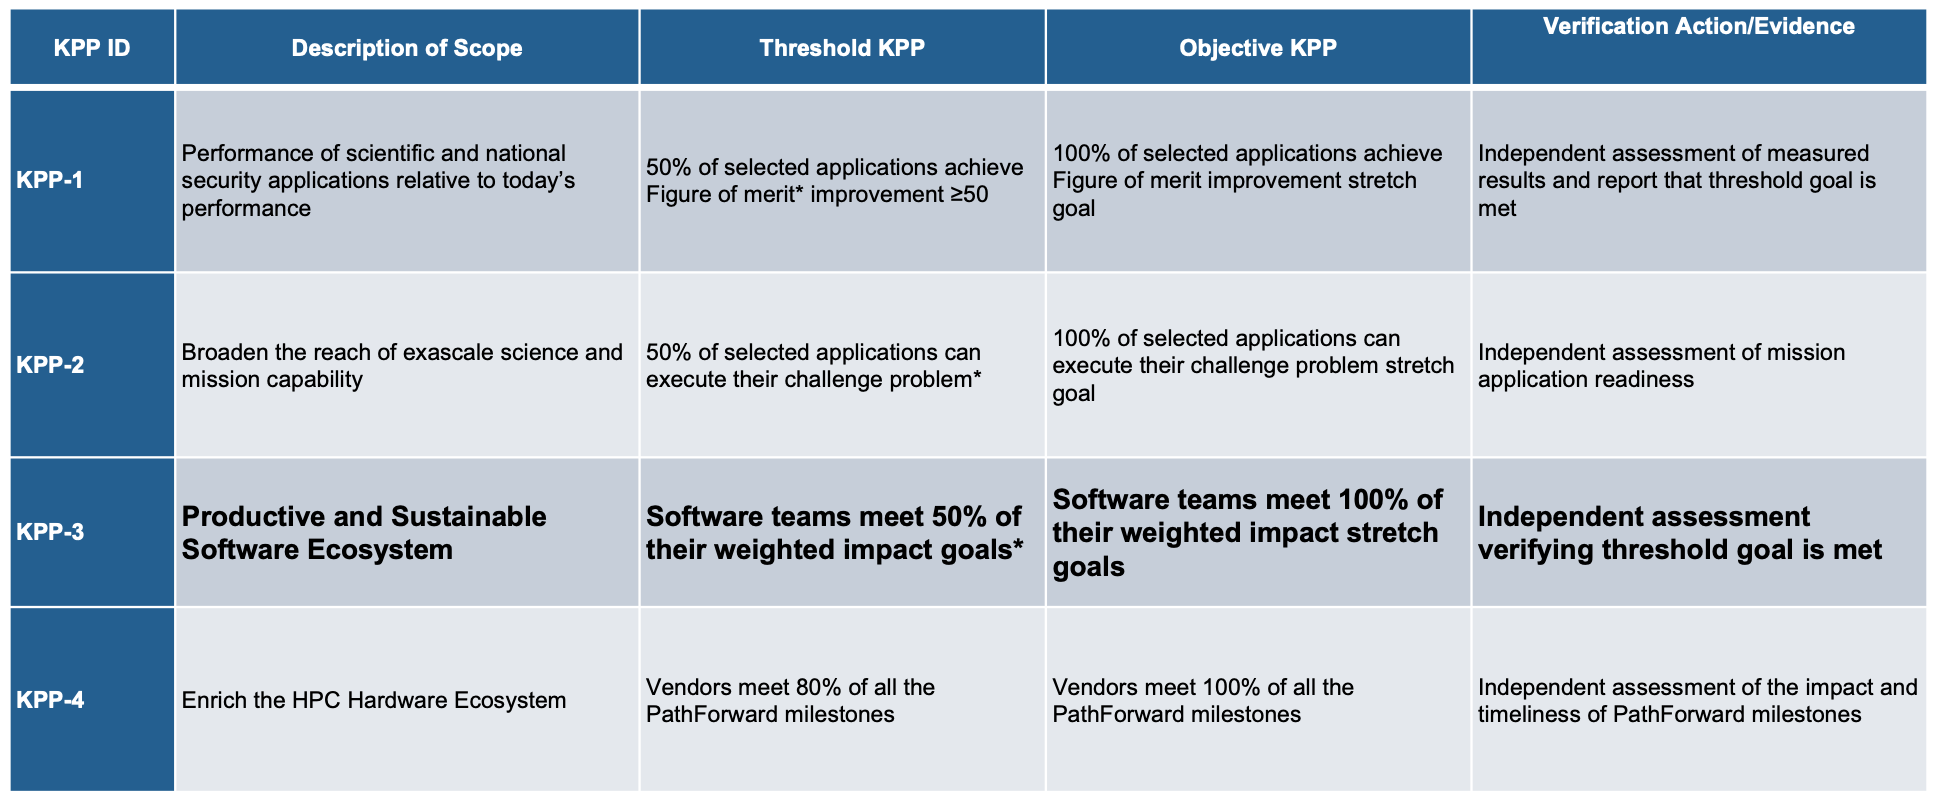
\includegraphics[width=0.9\linewidth]{KPP-Definitions}}
	\caption{ECP has four key performance parameters (KPPs).  ECP ST is the primary owner (with ECP AD co-design subprojects) of KPP-3.}
	\label{fig:kpp-definitions}
\end{figure}



First, we define terms:
\begin{itemize}
	\item \textbf{Capability:} Any significant product functionality, including existing features adapted to the pre-exascale and exascale environments, that can be integrated into a client environment.
	\item \textbf{Integration Goal:} A statement of impact on the ECP ecosystem where a software capability is used in a consequential and sustainable way by a client in pre-exascale environments first, then in exascale environments.  Integration goals are product focused.  A project that contributes to more than one product will have a KPP-3 Jira issue for each of its products.
	\item \textbf{Integration Score: }The number of successful capability integrations into a client environment.
	\item \textbf{Sustainable:} For the purposes of KPP-3, sustainable means that the capability is integrated in a way that reasonably assures future use of the capability beyond the end of ECP.  For libraries, this would generally mean that library usage is made from source code in the main repository and use of the library is tested regularly as a part of the client code regular regression testing.  For tools, sustainable would generally mean the tool is available as needed in the exascale environment.  For prototype capabilities that are incorporated into vendor and community software, the impact of the prototype is still visible to a subject matter expert.
\end{itemize}

\paragraph{Defining an Integration Goal}
Integration goals are defined per product within each project.  The goal statement will include:
\begin{itemize}
	\item The name of the product to which the project contributes.  The product must be listed in the ECP ST Product Dictionary.
	\item A description of the target clients into whose environments the product capabilities will be integrated.  Specific clients can be listed, but are not necessary.  Clients must be part of ECP, or otherwise part of the exascale systems ecosystem such as a vendor or facility partner.   
	\item A general description of the nature of the integration, addressing what it means to be successfully integrated.
\end{itemize}

\begin{table}[h!]
	\begin{tabular}{|L{1.5in}|L{2.0in}|L{2.5in}|}\hline
		\rowcolor{LightCyan}
		Integration Score & Capability & Integration Description\\\hline
		1 point per capability sustainably integrated by a client, per exascale platform used. &
		Complete, sustainable integration of a significant product capability into a client environment in a pre-exascale environment (tentative score) and in an exascale environment (confirmed score). &
		Client acknowledges benefit from product capability use and considers it part of their workflow. Integration is sustainable with documentation and testing. Integration of product capability into main product repo and SDK/E4S environments is completed.\\\hline
	\end{tabular}
	\caption{\label{table:KPP-3-scoring} Integration Goal Scoring: A point is accrued when a client integrates and sustainably uses a product's capabilities.  Scores are assessed annually.}
\end{table}


\paragraph{Demonstration and recording of progress toward integration goal}
All artifacts and evidence of progress will be captured in the Jira KPP-3 issue associated with a product integration goal as progress is made.  All integration scores are tentative until the capability is available and demonstrated in exascale environments.  Table~\ref{table:KPP-3-values} summarizes the defined values.

\begin{table}[h!]
	\begin{tabular}{|L{0.6in}|L{2.0in}|L{3.4in}|}\hline
		\rowcolor{LightCyan}
		Value & Definition & Description\\\hline
		Present & The current integration score. & This is always an indication of the progress the team has made. The present value is assessed annually.\\\hline
		Passing & The minimum integration score required for the product to be counted as part of ECP ST progress toward KPP-3. & The passing score is between 4 and 8 for each integration goal, 4 for larger integration efforts, 8 for smaller ones. This is equivalent to accomplishing one to two capability integration per year per product.\\\hline
		Stretch & The maximum reasonably achievable integration score for a product if capability integrations are successful with all potential ECP clients.   & The stretch value allows us to see the overall integration potential.\\\hline
	\end{tabular}
	\caption{\label{table:KPP-3-values} Key metric values: These values are determined by the L4 sub-project team when defining their KPP-3 issue.}
\end{table}

\paragraph{Assessment process}
While progress is recorded as it is achieved, progress assessment is done annually, including input from external subject matter experts (SMEs).  ECP leadership and SMEs will review integration score evidence, confirming or adjusting integration scores.
Note: Assessment can result in a reduced integration score from a previous year if a client has stopped using a capability that was previously used.

\paragraph{Transition from tentative to confirmed integration score}
Each integration score is tentative until the capability is available and demonstrated to be effective in the exascale environments.  Demonstration can be achieved by a variety of means such that ECP Leadership and SMEs are reasonably certain the capability positively impacts the client in exascale environments.  At this point the integration score becomes confirmed. 
Typically, the transition from tentative to confirmed would be a low-cost independent demonstration, or accomplished within the client’s environment as the client is conducting its own assessments. 
Note: The planned exascale system (El Capitan) that can support National Security applications will not be available until the end of FY23. Integration of ST products into National Security Applications will be considered for transition from tentative to confirmed when either a) evidence of integration is provided during FY20-22 ASC L1 and L2 milestones related to ECP/ATDM National Security application readiness for exascale platforms, and/or b) integration is demonstrated on the El Capitan early access systems, and exercises capabilities similar to those anticipated to be important to effectively using El Capitan.  For KPP-3 capability integrations targeted at El Capitan, we will use the best available confirmation process in FY23.
KPP-3 weighted scoring

\begin{table}[h!]
	\begin{tabular}{|L{1.0in}|L{0.5in}|L{4.5in}|}\hline
		\rowcolor{LightCyan}
		Impact Level & Weight & Comments\\\hline
		High & 2 & The score for integration goals associated with high impact products will be added to the KPP-3 score with a weight of 2.\\\hline
		Normal & 1 & Most KPP-3 Jira issues will have a weight of one.\\\hline
		Risk-Mitigating & 0.5 & Some KPP-3 Jira issues are associated with products that help us plan for the potential risks if high impact products don’t deliver as expected.\\\hline
		Shared  & 0.5 & Some projects receive funding from both NNSA and SC, e.g. RAJA/Kokkos. For these projects, the score is balanced to reflect dual contributions.\\\hline
	\end{tabular}
	\caption{\label{table:KPP-3-impact} Each integration score will have an associated weight depending on the potential impact if integration targets are not met.}
\end{table}

The KPP-3 score is the weighted sum of all integration goals that have an integration score that meets or exceeds its passing value. 
The KPP-3 score will initially be tentative.  The KPP-3 score is not officially met until the weighted sum of confirmed integration scores exceeds 50% of the total possible points.


\subsubsection{ECP ST Software Delivery}
An essential activity for, and the ultimate purpose of, ECP ST is the delivery of a software stack that enables productive and sustainable Exascale computing capabilities for target ECP applications and platforms, and the broader high-performance computing community. The ECP ST Software Ecosystem and Delivery sub-element (WBS 2.3.5) and the SDKs in each other sub-element provide the means by which ECP ST will deliver its capabilities.
\paragraph{ECP ST Delivery and HI Deployment}
Providing the ECP ST software stack to ECP applications requires coordination between ECP ST and ECP HI. The focus areas have a complementary arrangement where ECP ST delivers its products and ECP HI deploys them. Specifically:
\begin{itemize}
	\item ST \textbf{delivers} software.  ECP ST products are delivered directly to application teams, to vendors and to facilities.  ECP ST designs and implements products to run on DOE computing facilities platforms and make products available as source code via GitHub, GitLab or some other accessible repository.
	\item HI facilitates efforts to \textbf{deploy} ST (and other) software on Facilities platforms by installing it where users expect to find it. This could be in /usr/local/bin or similar directory, or available via “module load”.
\end{itemize}
Separating the concerns of delivery and deployment is essential because these activities require different skill sets. Furthermore, ECP ST delivers its capabilities to an audience that is beyond the scope of specific Facilities’ platforms. This broad scope is essential for the sustainability of ECP ST products, expanding the user and developer communities needed for vitality. In addition, ECP HI, the computer system vendors and other parties provide deployable software outside the scope of ECP ST, therefore having the critical mass of skills to deploy the entire software stack.

\paragraph{ECP ST Delivery Strategy}
ECP ST delivers it software products as source code, primarily in repositories found on GitHub, Gitlab installations or similar platforms. Clients such as ECP HI, OpenHPC and application developers with direct repository access then take the source and build, install and test our software. The delivery strategy is outlined in Figure~\ref{fig:softwarestack}.  

Users access ECP ST products using these basic mechanisms:
\begin{itemize}
	\item \textbf{Build from source code:} The vast majority of ECP ST products reach at least some of their user base via direct source code download from the product repository.  In some cases, the user will download a single compressed file containing product source, then expand the file to expose the collection of source and build files.  Increasingly, users will fork a new copy of an online repository.  After obtaining the source, the user executes a configuration process that detects local compilers and libraries and then builds the product.  This kind of access can represent a barrier for some users, since the user needs to build the product and can encounter a variety of challenges in that process, such as an incompatible compiler or a missing third-party library that must first be installed.  However, building from source can be a preferred approach for users who want control over compiler settings, or want to adapt how the product is used, for example, turning on or off optional features, or creating adaptations that extend product capabilities.  For example, large library frameworks such as PETSc and Trilinos have many tunable features that can benefit from the user building from source code.  Furthermore, these frameworks support user-defined functional extensions that are easier to support when the user builds the product from source.  ECP ST is leveraging and contributing to the development of Spack~\cite{gamblin+:sc15}.  Via meta-data stored in a Spack \textit{package} defined for each product, Spack leverages a product's native build environment, along with knowledge about its dependencies, to build the product and dependencies from source.  Spack plays a central role in ECP ST software development and delivery processes by supporting turnkey builds of the ECP ST software stack for the purposes of continuous integration testing, installation and seamless multi-product builds.
	\item \textbf{DOE computing facilities:} Each DOE computing facility (ALCF, OLCF, NERSC, LLNL and ACES [LANL/SNL]) provides pre-built versions of 17 to 20 ECP ST products (although the exact mix of products varies somewhat at each site).  Many of these products are what users would consider to be part of the core system capabilities, including compilers, e.g., Flang (Section~\ref{subsubsect:flang}) and LLVM (Section~\ref{subsubsect:sollve}), and parallel programming environments such as MPICH (Section~\ref{subsubsect:mpich}), OpenMPI (Section~\ref{subsubsect:openmpi}) and OpenMP (Section~\ref{subsubsect:bolt}).  Development tools such as PAPI (Section~\ref{subsubsect:exapapi}) and TAU (Section~\ref{subsubsect:tau}) are often part of this suite, if not already included in the vendor stack. Math and data libraries such as PETSc (Section~\ref{subsubsect:petsc}), Trilinos (Section~\ref{subsubsect:peeks}), HDF5 (Section~\ref{subsubsect:exahdf5}) and others are also available in some facilities software installations.  We anticipate and hope for increased collaboration with facilities via the ECP Hardware \& Integration (HI) Focus Area.  We are also encouraged by multi-lab efforts such as the Tri-Lab Operating System Stack (TOSS)~\cite{TOSS} that are focused on improving uniformity of software stacks across facilities.
	\item \textbf{Vendor stacks:} Computer system vendors leverage DOE investments in compilers, tools and libraries.  Of particular note are the wide use of MPICH(Section~\ref{subsubsect:mpich}) as software base for most HPC vendor MPI implementations and the requirements, analysis, design and prototyping that ECP ST teams provide.  Section~\ref{subsection:external-contributions} describes some of these efforts.
	\item \textbf{Binary distributions:} Approximately 10 ECP ST products are available via binary distributions such as common Linux distributions, in particular via OpenHPC\cite{OpenHPC}.  ECP ST intends to foster growth of availability via binary distributions as an important way to increase the size of the user community and improve product sustainability via this broader user base.
\end{itemize}

\begin{figure}
	\centering
	\includegraphics[width=0.9\linewidth]{SoftwareStack}
	\caption{\textbf{The ECP ST software stack is delivered to the user community through several channels.} Key channels are via source code, increasingly using SDKs, direct to Facilities in collaboration with ECP HI, via binary distributions, in particular the OpenHPC project and via HPC vendors.  The SDK leadership team includes  ECP ST team members with decades of experience delivering scientific software products.}
	\label{fig:softwarestack}
\end{figure}



%\newpage
%\section{ECP ST Technical Areas}
%\subsection{\stid{1}  \pmr}\label{subsect:pmr}

\textbf{End State:} A cross-platform, production-ready programming environment that enables and accelerates the development of mission-critical software at both the node and full-system levels.

\subsubsection{Scope and Requirements}
A programming model provides the abstract design upon which developers express and coordinate the efficient parallel execution of their program. A particular model is implemented as a developer-facing interface and a supporting set of runtime layers. To successfully address the challenges of exascale computing, these software capabilities must address the challenges of programming at both the node- and full-system levels. These two targets must be coupled to support multiple complexities expected with exascale systems (e.g., locality for deep memory hierarchies, affinity for threads of execution, load balancing) and also provide a set of mechanisms for performance portability across the range of potential and final system designs. Additionally, there must be mechanisms for the interoperability and composition of multiple implementations (e.g., one at the system level and one at the node level). This must include abilities such as resource sharing for workloads that include coupled applications, supporting libraries and frameworks, and capabilities such as in situ analysis and visualization. 

Given the ECP’s timeline, the development of new programming languages and their supporting infrastructure is infeasible. We do, however, recognize that the augmentation or extension of the features of existing and widely used languages (e.g., C/C++ and Fortran) could provide solutions for simplifying certain software development activities. 

\subsubsection{Assumptions and Feasibility}
The intent of the PMR L3 is to provide a set of programming abstractions and their supporting implementations that allow programmers to select from options that meet demands for expressiveness, performance, productivity, compatibility, and portability. It is important to note that, while these goals are obviously desirable, they must be balanced with an additional awareness that today’s methods and techniques may require changes in both the application and the overall programming environment and within the supporting software stack.

\subsubsection{Objectives}
PMR provides the software infrastructure necessary to enable and accelerate the development of HPC applications that perform well and are correct and robust, while reducing the cost both for initial development and ongoing porting and maintenance. PMR activities need to reflect the requirements of increasingly complex application scenarios, usage models, and workflows, while at the same time addressing the hardware challenges of increased levels of concurrency, data locality, power, and resilience. The software environment will support programming at multiple levels of abstraction that includes both mainstream as well as alternative approaches if feasible in ECP’s timeframe. 

Both of these approaches must provide a portability path such that a single application code can run well on multiple types of systems, or multiple generations of systems, with minimal changes. The layers of the system and programming environment implementation will therefore aim to hide the differences through compilers, runtime systems, messaging standards, shared-memory standards, and programming abstractions designed to help developers map algorithms onto the underlying hardware and schedule data motion and computation with increased automation.
\subsubsection{Plan}
PMR contains nine L4 projects. To ensure relevance to DOE missions, these efforts leverage and collaborate with existing activities within the broader HPC community. The PMR area supports the research and development needed to produce exascale-ready versions of the Message Passing Interface (MPI);  Partitioned Global-Address Space Libraries (UPC++, GASNet); task-based programming models (Legion, PaRSEC); software for node-level performance portability (Kokkos, RAJA); and libraries for memory, power, and resource management.
Initial efforts focused on identifying the core capabilities needed by the selected ECP applications and components of the software stack, identifying shortcomings of current approaches, establishing performance baselines of existing implementations on available petascale and prototype systems, and the re-implementation of the lower-level capabilities of relevant libraries and frameworks. These efforts provided demonstrations of parallel performance of algorithms on pre-exascale, leadership-class machines--at first on test problems, but eventually in actual applications (in close collaboration with the AD and HI teams). Initial efforts also informed research into exascale-specific algorithms and requirements that will be implemented across the software stack. The supported projects targeted and implemented early versions of their software on CORAL, NERSC and ACES pre-exascale systems--with an ultimate target of production-ready deployment on the exascale systems.
In FY20--23, the focus will be on development and tuning for the specific architectures of the selected exascale platforms, in addition to tuning specific features that are critical to ECP applications.

Throughout the effort, the applications teams and other elements of the software stack evaluate and provide feedback on their functionality, performance, and robustness. Progress towards these goals is documented quarterly and evaluated annually (or more frequently if needed) based on PMR-centric milestones as well as joint milestone activities shared across associated software stack activities by Application Development and Hardware \& Integration focus areas.


\subsubsection{Risks and Mitigation Strategies}
The mainstream activities of ECP in the area of programming models focus on advancing the capabilities of MPI and OpenMP. Pushing them as far as possible into the exascale era is key to supporting an evolutionary path for applications. This is the primary risk mitigation approach for existing application codes. Extensions to MPI and OpenMP standards require research, and part of the efforts will focus on rolling these findings into existing standards, which takes time. To further address risks, PMR is exploring alternative approaches to mitigate the impact of potential limitations of the MPI and OpenMP programming models. 

Another risk is the failure of adoption of the software stack by the vendors, which is mitigated by the specific delivery focus in sub-element SW Ecosystem and Delivery. Past experience has shown that a combination of laboratory-supported open-source software and vendor-optimized solutions built around standard APIs that encourage innovation across multiple platforms is a viable approach and is what we are doing in PMR. We are using close interaction with the vendors early on to encourage adoption of the software stack, including well-tested practices of including support for key software products or APIs into large procurements through NRE or other contractual obligations. A mitigation strategy for this approach involves building a long-lasting open-source community around projects that are supported via laboratory and university funding. 

Creating a coordinated set of software requires strong management to ensure that duplication of effort is minimized. This is recognized by ECP management, and processes are in place to ensure collaboration is effective, shortcuts are avoided unless necessary, and an agile approach to development is instituted to prevent prototypes moving directly to product. 

\subsubsection{Future Trends}
Recently announced exascale system procurements have shown that the
trend in exascale compute-node hardware is toward heterogeneity:
Compute nodes of future systems will have a combination of regular
CPUs and accelerators (typically GPUs). Furthermore, the GPUs will not
be just from NVIDIA as on existing systems: One system will have Intel
GPUs and another will have AMD GPUs. In other words, there will be a
diversity of GPU architectures, each with their own vendor-preferred
way of programming the GPUs. An additional complication
is that although the HPC community has some experience in using NVIDIA
GPUs and the associated CUDA programming model, the community has relatively
little experience in programming Intel or AMD GPUs.  These
issues lead to challenges for application and software teams in
developing exascale software that is both portable and high performance. Below
we outline trends in programming these complex systems that will help
alleviate some of these challenges.

\paragraph{Trends in Internode Programming}
The presence of accelerator hardware on compute nodes has resulted in individual
compute nodes becoming very powerful. As a result, millions of compute
nodes are no longer needed to build an exascale system. This trend
results in a lower burden on the programming system used for internode
communication. It is widely expected that MPI will continue to serve
the purpose of internode communication on exascale systems and is the
least disruptive path for applications, most of which already use
MPI. Nonetheless, improvements are needed in the MPI Standard as well
as in MPI implementations in areas such as hybrid programming
(integration with GPUs and GPU memory, integration with the intranode
programming model), overall resilience and robustness, scalability,
low-latency communication, optimized collective algorithms, optimized support
for exascale interconnects and lower-level communication paradigms
such as OFI and UCX, and scalable process startup and management. PGAS
models, such as UPC++ and OpenSHMEM, are also available to be used by
applications that rely on them and face similar
challenges as MPI on exascale systems. These challenges are being tackled by the MPI and
UPC++/GASNet projects in the PMR area.

\paragraph{Trends in Intranode Programming}
The main challenge for exascale is in achieving performance and portability for
intranode programming, for which a variety of options
exist. Vendor-supported options include CUDA and OpenACC for NVIDIA
GPUs, SYCL/DPC++ for Intel GPUs, and HIP for AMD GPUs. OpenACC
supports accelerator programming via compiler directives. SYCL
provides a C++ abstraction on top of OpenCL, which itself is a
portable, lower-level API for programming heterogeneous
devices. Intel's DPC++ is similar to SYCL with some extensions. HIP
from AMD is similar to CUDA; in fact, AMD provides translation tools
to convert CUDA programs to HIP.

Among portable, standard programming models, OpenMP has supported
accelerators via the \texttt{target} directive starting with OpenMP version
4.0 released in July 2013. Subsequent releases of OpenMP (version 4.5
and 5.0) have further improved support for accelerators. OpenMP is
supported by vendors on all platforms and, in theory, could serve as a
portable intranode programming model for systems with
accelerators. However, in practice, a lot depends on the quality of
the implementation.

Kokkos and RAJA provide another alternative for portable,
heterogenous-node programming via C++ abstractions. They
are designed to work on complex node architectures
with multiple types of execution resources and multilevel memory
hierarchies. Many ECP applications are successfully using Kokkos and
RAJA to write portable parallel code that runs efficiently on GPUs.

We believe these options (and high-quality implementations of them) will
meet the needs of applications in the exascale timeframe. 

%\subsection{\stid{2} \tools}\label{subsect:tools}

\textbf{End State:}	A suite of development tools and supporting unified infrastructure aimed at improving developer productivity across increasingly complex architectures, especially those targeted for Exascale platforms.


\subsubsection{Scope and Requirements}
For Exascale systems, the compilers, profilers, debuggers, and other software development tools must be increasingly sophisticated to give software developers insight into the behavior of not only the application and the underlying hardware but also the details corresponding to the underlying programming model implementation and supporting runtimes (e.g., capturing details of locality and affinity). These capabilities should be enhanced with further integration into the supporting compiler infrastructure and lower layers of the system software stack (e.g., threading, runtime systems, and data transport libraries), and hardware support. Most of the infrastructure will be released as open source, as many of them already are, with a supplementary goal of transferring the technology into commercial products. Given the diversity of Exascale systems architectures, some subset of the tools may be specific to one or more architectural features and is potentially best implemented and supported by the vendor; however, the vendor will be encouraged to use open APIs to provide portability, additional innovation, and integration into the tool suite and the overall software stack.


\subsubsection{Assumptions and Feasibility }

The overarching goal of improving developer productivity for Exascale platforms introduces new issues of scale that will require more lightweight methods, hierarchical approaches, and improved techniques to guide the developer in understanding the characteristics of their applications and to discover sources of the errors and performance issues. Additional efforts for both static and dynamic analysis tools to help identify lurking bugs in a program, such as race conditions, are also likely needed. The suite of needed capabilities spans interfaces to hardware-centric resources (e.g., hardware counters, interconnects, and memory hierarchies) to a scalable infrastructure that can collect, organize, and distill data to help identify performance bottlenecks and transform them into an actionable set of steps and information for the software developer. Therefore, these tools share significant challenges due to the increase in data and the resulting issues with management, storage, selection, analysis, and interactive data exploration. This increased data volume stems from multiple sources, including increased concurrency, processor counts, additional hardware sensors and counters on the systems, and increasing complexity in application codes and workflows.

Compilers obviously play a fundamental role in the overall programming environment but can also serve as a powerful entry point for the overall tool infrastructure. In addition to optimizations and performance profiling, compiler-based tools can help with aspects of correctness, establishing connections between programming model implementations and the underlying runtime infrastructures, and auto-tuning. In many cases, today's compiler infrastructure is proprietary and closed source, limiting the amount of flexibility for integration and exploration into the Exascale development environment. In addition to vendor compiler options, this project aims to provide an open source compiler capability that can play a role in better supporting and addressing the challenges of programming at Exascale. 


\subsubsection{Objectives}

This project will design, develop, and deploy an Exascale suite of development tools built on a unified infrastructure for development, analysis, and optimization of applications, libraries, and infrastructure from the programming environments of the project. The overarching goal is to leverage and integrate the data measurement, acquisition, storage, and analysis and visualization techniques being developed in other projects of the software stack. The project will seek to leverage techniques for common and identified problem patterns and create new techniques for data exploration related to profiling and debugging and support advanced techniques such as autotuning and compiler integration. We will seek to establish an open-source compiler activity leveraging activities around the LLVM infrastructure. These efforts will require collaboration and integration with system monitoring and various layers within the software stack.


\subsubsection{Plan}
It is expected that multiple projects will be supported under the tools effort. To ensure relevance to DOE missions, most of these efforts shall be DOE laboratory led and leverage and collaborate with existing activities within the broader HPC community. Initial efforts will focus on identifying the core capabilities needed by the selected ECP applications, components of the software stack, expected hardware features, and the selected industry activities from within the Hardware and Integration focus area. The supported projects will target and implement early versions of their software on both CORAL and APEX systems, with an ultimate target of production-ready deployment on the Exascale systems. Throughout this effort the applications teams and other elements of the software stack will evaluate and provide feedback on their functionality, performance, and robustness. These goals will be evaluated yearly (or more often as needed) based on milestones as well as joint milestone activities shared across the associated software stack activities by AD and HI focus areas.

\subsubsection{Risks and Mitigations Strategies}

A risk exists in terms of adoption of the various tools and their supporting infrastructure by the broader community, including support by system vendors. Past experience has shown that a combination of laboratory-supported open source software and vendor-optimized solutions built around standard APIs that encourage innovation across multiple platforms is a viable approach, and this will be undertaken. We will track this risk primarily via the risk register.

Given its wide use within a range of different communities, and its modular design principles, the project's open source compiler activities will focus on the use of the LLVM compiler infrastructure as a path to reduce both scope and complexity risks and leverage with an already established path for NRE investments across multiple vendors. The compilers and their effectiveness are tracked in the risk register. 

Another major risk for projects in this area is the lack of low-level access to hardware and software necessary for using emerging architectural features. Many of these nascent architectural features have immature implementations and software interfaces that must be refined prior to release to the broader community. This project should be at the forefront of this interaction with early delivery systems. This risk is also tracked in the risk register for compilers, which are particularly vulnerable.

\subsubsection{Future Trends}

Future architectures are becoming more heterogeneous and complex~\cite{vetter:2018:extreme}. As such, the role of languages, compilers, runtime systems, and performance and debugging tools will becoming increasingly important for productivity and performance portability. 
%
In particular, our ECP strategy focuses on improving the open source LLVM compiler and runtime ecosystem; LLVM has gained considerable traction in the vendor software community, and it is the core of many existing heterogeneous compiler systems from NVIDIA, AMD, Intel, ARM, IBM, and others.  We foresee that this trend will continue, which is why we have organized the \tools\ technical area around LLVM-oriented projects.  
%
Many of our contributions to LLVM address these trends and will persist after ECP ends. 
%
For example, our contributions for directive-based features for heterogeneous computing (e.g., OpenMP, OpenACC) will not only provide direct capabilities to ECP applications, but it will also impact the redesign and optimization of the LLVM infrastructure to support heterogeneous computing.
%
In a second example, Flang (open source Fortran compiler for LLVM; [the second version is also known as F18]) will become increasingly important to the worldwide Fortran application base, as vendors find it easier to maintain and deploy to their own Fortran frontend (based on Flang).  
%
Furthermore, as Flang become increasingly robust, researchers and vendors developing new architectures will have immediate access to Flang, making initial Fortran support straightforward in ways similar to what we are seeing in Clang as the community C/C++ frontend.

%

%\subsection{\stid{3} \mathlibs}\label{subsect:mathlibs}

\textbf{End State:} Mathematical libraries that (i) interoperate with the ECP software stack; (ii) are incorporated into the ECP applications; and (iii) provide scalable, resilient numerical algorithms that facilitate efficient simulations on Exascale computers.

\subsubsection{Scope and Requirements}
Software libraries are powerful means of sharing verified, optimized algorithms and their implementations. Applied research, development, and support are needed to extend existing DOE mathematical software libraries to make better use of Exascale architectural features. DOE-supported libraries encapsulate the latest results from mathematics and computer science R\&D; many DOE mission-critical applications rely on these numerical libraries and frameworks to incorporate the most advanced technologies available. 

The Mathematical Libraries effort will ensure the healthy functionality of the numerical software libraries on which the ECP applications will depend. The DOE mathematical software libraries used by computational science and engineering applications span the range from light-weight collections of subroutines with simple APIs to more “end-to-end” integrated environments and provide access to a wide range of algorithms for complex problems.

Advances in mathematical and scientific libraries will be necessary to enable computational science on Exascale systems. Exascale computing promises not only to provide more computational resources enabling higher-fidelity simulations and more demanding studies but also to enable the community to pose new scientific questions. Exascale architectural characteristics introduce new features that algorithms and their implementations will need to address in order to be scalable, efficient, and robust. As a result, it will be necessary to conduct research and development to rethink, reformulate, and develop existing and new methods and deploy them in libraries that can be used by applications to deliver more complete and sophisticated models and provide enhanced predictive simulation and analysis capabilities.

The Mathematical Libraries effort must (1) collaborate closely with the Application Development effort (WBS 2.2) to be responsive to the needs of the applications and (2) collaborate with the other products within the Software Technology effort (WBS 2.3) in order to incorporate new technologies and to provide requirements. All software developed within the Mathematical Libraries effort must conform to best practices in software engineering, which will be formulated early in the project in collaboration with the Applications Development focus area. Software produced by this effort must provide scalable numerical algorithms that enable the application efforts to reach their performance goals, encapsulated in libraries whose data structures and routines can be used to build application software.

\subsubsection{Assumptions and Feasibility}
Years of DOE investment have led to a diverse and complementary collection of mathematical software, including AMReX, Chombo, hypre, Dakota, DTK, MAGMA, MFEM, PETSc/TAO, PLASMA, ScaLAPACK, SUNDIALS, SuperLU, and Trilinos. This effort is evolving a subset of existing libraries to be performant on Exascale architectures. In addition, research and development is needed into new algorithms whose benefits may be seen only at the extreme scale. Results of preliminary R\&D projects indicate that this approach is feasible.

Additionally, ECP will need to rely on a strong, diverse, and persistent base math research program, which is assumed to continue being supported by the DOE-SC ASCR Office. The ECP technical directors will schedule quarterly meetings with the ASCR research program managers to get updates on research results that might meet ECP requirements as well as to inform the program managers of ECP needs in applications and software components.

\subsubsection{Objectives}
The high-level objective of the Mathematical Libraries effort is to provide scalable, resilient numerical algorithms that facilitate efficient application simulations on Exascale computers. To the greatest extent possible, this objective should be accomplished by preserving the existing capabilities in mathematical software while evolving the implementations to run effectively on the Exascale systems and adding new capabilities that may be needed by Exascale applications.

The key performance metrics for the software developed by this effort are scalability, efficiency, and resilience. As a result of the new capabilities in mathematics libraries developed under this effort, applications will tackle problems that were previously intractable and will model phenomena in physical regimes that were previously unreachable.

\subsubsection{Plan}
As detailed below, the Mathematical Libraries effort supports six complementary L4 projects as needed to meet the needs of ECP applications. These efforts include strong collaborations among DOE labs, academia, industry, and other organizations, and leveraging existing libraries that are widely used by the DOE HPC community. 

Initial efforts have focused on identifying core capabilities needed by selected ECP applications, establishing performance baselines of existing implementations on available Petascale and prototype systems, and beginning re-implementation of lower-level capabilities of the libraries and frameworks. Another key activity is collaborating across all projects in the Mathematical Libraries effort to define community policies in order to enable compatibility among complementary software and to provide a foundation for future work on deeper levels of interoperability. Refactoring of higher-level capabilities will be prioritized based on needs of the applications. In time, these efforts will provide demonstrations of parallel performance of algorithms from the mathematical software on pre-Exascale, leadership-class machines (at first on test problems, but eventually in actual applications). The initial efforts also are informing research into advanced exascale-specific numerical algorithms that will be implemented within the libraries and frameworks. In FY20–23, the focus will be on development and tuning for the specific architectures of the selected exascale platforms, in addition to tuning specific features that are critical to ECP applications. The projects will implement their software on the CORAL, NERSC and ACES systems, and ultimately on initial Exascale systems, so that functionality, performance, and robustness can be evaluated by the applications teams and other elements of the software stack. Throughout the effort the applications teams and other elements of the software stack will evaluate and provide feedback on their functionality, performance, and robustness. These goals will be evaluated at least yearly based on milestones as well as joint milestone activities shared across the associated software stack activities by Application Development and Hardware and Integration project focus areas.


\subsubsection{Risks and Mitigations Strategies}
There are a number of foreseeable risks associated with the Mathematical Libraries effort.
\begin{itemize}
	\item Efficient implementation of new or refactored algorithms to meet Exascale computing requirements may introduce unanticipated requirements on programming environments. To mitigate this risk, effective communication is needed between projects in the Mathematical Libraries effort and projects tasked with developing the programming environments. From the application perspective, this is specifically tracked in a specific AD risk the risk register. Additionally, the risks of an inadequate programming environment overall are tracked as a specific ST risk in the risk register.
	\item A significant number of existing algorithms currently implemented in numerical libraries may scale poorly, thereby requiring significantly more effort than refactoring. The R\&D planned for the first three years of the ECP is the first mitigation for this risk (as well as the co-design centers planned in Application Development). In addition, the ECP will be able to draw from a strong, diverse, well-run, persistent base math research program. From the application perspective, this is tracked via an AD risk in the risk register. Scaling issues for the software stack in general, including libraries, are monitored via an ST risk in the risk register.
	\item Exascale architecture characteristics may force a much tighter coupling among the models, discretizations, and solvers employed, causing general-purpose solvers to be too inefficient. The mitigation strategy is to ensure close collaboration with the sub-elements of the Application Development focus area (WBS 2.2) to understand integration and coupling issues. Again, a strong, diverse, well-run, persistent base math research program may provide risk mitigation strategies.
\end{itemize}

\subsubsection{Future Trends}
Mathematical libraries have been one of the strongest success stories in the scientific software ecosystem.  These libraries encode specialized algorithms on advanced computers that can be the difference between success or not.  Algorithms such as multigrid, highly-tuned dense linear algebra and optimized FFTs, can improve performance by orders of magnitude and reduce the asymptotic algorithmic complexity for users.  We foresee that math libraries will have an ever-growing role in the scientific software ecosystem, as architectures become more challenging for targeting optimization and algorithms require even more concurrency and latency hiding in order to realize performance on modern computer systems.

In addition, we anticipate that new algorithms based on multi-precision arithmetic will further enable performance improvements on compute devices that are optimized for machine learning workloads, where short precision can be an order of magnitude faster that double precision.  

For a deeper discussion of the futures of ECP Math Libraries efforts, please consult the paper ``Preparing Sparse Solvers for Exascale Computing''~\cite{ECP-Solvers}.
%\subsection{\stid{4} \dataviz}\label{subsect:dataviz}

\textbf{End State:} A production-quality storage infrastructure necessary to manage, share, and facilitate analysis of data in support of mission critical codes. Data analytics and visualization software that effectively supports scientific discovery and understanding of data produced by Exascale platforms.

\subsubsection{Scope and Requirements}
Changes in the hardware architecture of Exascale supercomputers will render current approaches to data management, analysis and visualization obsolete, resulting in disruptive changes to the scientific workflow and rendering traditional checkpoint/restart methods infeasible. A major concern is that Exascale system concurrency is expected to grow by five or six orders of magnitude, yet system memory and input/output (I/O) bandwidth/persistent capacity are only expected to grow by one and two orders of magnitude, respectively. The reduced memory footprint per FLOP further complicates these problems, as does the move to a hierarchical memory structure. Scientific workflow currently depends on exporting simulation data off the supercomputer to persistent storage for post-hoc analysis.

On Exascale systems, the power cost of data movement and the worsening I/O bottleneck will make it necessary for most simulation data to be analyzed in situ, or on the supercomputer while the simulation is running. Furthermore, to meet power consumption and data bandwidth constraints, it will be necessary to sharply reduce the volume of data moved on the machine and especially the data that are exported to persistent storage. The combination of sharp data reduction and new analysis approaches heighten the importance of capturing data provenance (i.e., the record of what has been done to data) to support validation of results and post-hoc data analysis and visualization.
Data and Visualization is the title for Data Management (DM) \& Data Analytics and Visualization (DAV) activities in the Exascale project.

Data management (DM) activities address the severe I/O bottleneck and challenges of data movement by providing and improving storage system software; workflow support including provenance capture; and methods of data collection, reduction, organization and discovery.

Data analytics and visualization (DAV) are capabilities that enable scientific knowledge discovery. Data analytics refers to the process of transforming data into an information-rich form via mathematical or computational algorithms to promote better understanding. Visualization refers to the process of transforming scientific simulation and experimental data into images to facilitate visual understanding. Data analytics and visualization have broad scope as an integral part of scientific simulations and experiments; they are also a distinct separate service for scientific discovery, presentation and documentation purposes, as well as other uses like code debugging, performance analysis, and optimization. 

The scope of activities falls into the following categories:
\begin{itemize}
\item Scalable storage software infrastructure – system software responsible for reliable storage and retrieval of data supporting checkpointing, data generation, and data analysis I/O workloads
\item Workflow and provenance infrastructure – facilitating execution of complex computational science processes and the capture and management of information necessary to interpret and reproduce results
\item Data collection, reduction, and transformation – enabling complex transformation and analysis of scientific data where it resides in the system and as part of data movement, in order to reduce the cost to solution
\item Data organization and discovery – indexing and reorganizing data so that relevant items can be identified in a time- and power-efficient manner, and complex scientific data analysis can be performed efficiently on Exascale datasets
\item In situ algorithms and infrastructure – performing DAV while data is still resident in memory as the simulation runs enabling automatic identification, selection and data reduction for Exascale applications.
\item Interactive post-hoc approaches – on data extracts that produced in situ and support post-hoc understanding through exploration.
\item Distributed memory multi-core and many-core approaches, for the portable, performant DM and DAV at Exascale.
\end{itemize}
\subsubsection{Assumptions and Feasibility}
\begin{itemize}
\item Scaling up traditional DM and DAV approaches is not a viable approach due to severe constraints on available memory and I/O capacity, as well as dramatically different processor and system architectures being at odds with contemporary DAV architectures.
\item Simulations will produce data that is larger and more complex, reflecting advances in the underlying physics and mathematical models. Science workflows will remain complex, and increasing requirements for repeatability of experiments, availability of data, and the need to find relevant data in Exascale datasets will merit advances in workflow and provenance capture and storage.
\item The expense of data movement (in time, energy, and dollars) will require data reduction methods, shipping functions to data, and placing functionality where data will ultimately reside.
\item Solid-state storage will become cheaper, denser, more reliable, and more ubiquitous (but not cheap enough to replace disk technology in the Exascale timeframe). Exascale compute environments will have in-system nonvolatile storage and off-system nonvolatile storage in addition to disk storage. Applications will need help to make use of the complex memory/storage architectures.
\item Disks will continue to gain density but not significant bandwidth; disks will become more of a capacity solution and even less a bandwidth one.
\item Industry will provide parts of the overall data management, data analysis and visualization solution, but not all of it; non-commercial parts will be produced and maintained.
\item This plan and associated costs were formulated based on the past decade of DOE visualization and data analysis activities, including the successful joint industry/laboratory-based development of open-source visualization libraries and packages (VTK, VisIt, and ParaView).
\end{itemize}
\subsubsection{Objectives}
Data management, analysis and visualization software must provide:
\begin{itemize}
\item production-grade Exascale storage infrastructure(s), from application interfaces to low-level storage organization, meeting requirements for performance, resilience, and management of complex Exascale storage hierarchies;
\item targeted research to develop a production-grade in situ workflow execution system, to be integrated with vendor resource management systems, meeting science team requirements for user-defined and system-provided provenance capture and retention;
\item production-grade system-wide data transfer and reduction algorithms and infrastructure, with user interface and infrastructure for moving/reducing data within the system, to be integrated with vendor system services and meeting science and national security team requirements; and
\item production-grade metadata management enabling application and system metadata capture, indexing, identification, and retrieval of subsets of data based on complex search criteria and ensures that technologies target science and national security team requirements.
\item targeted research to develop a production-grade in situ algorithms, to be integrated with open source visualization and analysis tools and infrastructure, meeting science team data reduction requirements
\item targeted research to develop a production-grade algorithms for the new types of data that will be generated and analyzed on Exascale platforms as a result of increased resolution, evolving scientific models and goals, and increased model and data complexity.
\item targeted research to develop a production-grade post-hoc approach that support interactive exploration and understanding of data extracts produced by in situ algorithms
\item production-grade Exascale data analysis and visualization algorithms and infrastructure, meeting requirements for performance, portability and sustainability for evolving hardware architectures and software environments. 
\end{itemize}

\subsubsection{Plan}
Particularly in the area of DM, productization of technologies is a necessary step for adoption, research-quality software is not enough. One approach we will take is to fund vendors of products in related areas to integrate specific technologies into their product line. When developing objectives for this activity, a focus was placed on the availability of products that deliver these technologies on platforms of interest. Activities can be separated into two categories:
\begin{itemize}
\item Community/Coordination – designed to build the R\&D community, inform ourselves and the community regarding activities in the area, track progress, and facilitate coordination.
\item Targeted R\&D – filling gaps in critical technology areas (storage infrastructure, workflow, provenance, data reduction and transformation, and organization and discovery).
\end{itemize}
In the workflows area, the first 3 years of the project will identify existing software systems that are in use by the DOE community and are aimed at applications that require HPC systems (eventually Exascale systems) and support further R\&D to the emerging requirements of Exascale workflows as well as interaction with other parts of the software stack and adaptation to Exascale hardware architectures.

Portions of the DAV software stack are being productized and supported by industry, which will help to control costs in the long term. Activities to achieve the DAV objectives are heavily dependent on developments across the Exascale project, and thus close coordination with other teams is essential. Close engagement with application scientists is crucial to the success of DAV, both in terms of understanding and addressing the requirements of science at scale and ensuring that computational scientists are able to adopt and benefit from the DAV deliverables.

Many objectives need initial research projects to define plausible solutions. These solutions will be evaluated and progressively winnowed to select the best approaches for the Exascale machine and the needs of science. Selected projects will continue to receive support to extend their research and development efforts to integrate their solutions into the open-source Exascale software stack. 

\subsubsection{Risks and Mitigations Strategies}
There are specific risks identified for the Data and Visualization portfolio.  These risks are tracked in the risk register .  
\begin{itemize}
\item Application teams may continue to employ ad hoc methods for performing data management in their work, resulting in increased I/O bottlenecks and power costs for data movement. Application team engagement, working within the overall software stack, and input into Hardware Integration will be necessary if results are to be deployed, adopted, and significantly improve productivity.
\item Despite funding vendor activities, industry partners may determine the market is insufficient to warrant meeting Exascale requirements.
\item If vendor integration and targeted R\&D activities are not closely coordinated, gaps will not be effectively identified and targeted, or successful R\&D will not be integrated into industry products in the necessary timeframe.
\item Vendors supplying data management solutions are likely to be distinct from Exascale system vendors. Additional coordination will be necessary, beyond DM productization, in order to ensure interoperability of DM solutions with specific Exascale platforms.
\item Data management from an application perspective is tracked in one of the identified risks.  Additionally, the software stack tracks several risks indirectly related to data management as well.
\item Failure of scientists to adopt the new DAV software is a major risk that is exacerbated if the DAV software is research quality. Mitigating this risk depends on close engagement with domain scientists and supporting layers of the software stack through co-design activities, as well as investment in development and productization of DAV codes.
\item Redundant efforts in domain science communities and within ASCR-supported activities such as SciDAC result in wasted resources. Communication and close coordination provide the best strategy for mitigation.
\item Fierce industry and government competition for DAV experts creates a drain on laboratory personnel in DAV and makes lab hiring in this area difficult. Stable funding and a workforce development program would help to mitigate these risks.
\item A skilled workforce is required for a successful Exascale project.
\end{itemize}

\subsubsection{Future Trends}

\textbf{Graphics Architectures and Approaches}  Graphics architectures are improving in terms of raw computational power and through the addition of specialized libraries for accelerating ray-tracing, volume rendering, and denoising. Nvidia has added specialized hardware processing units for ray-tracing and machine learning to their GPU offerings.  Intel has developed a suite of CPU accelerated libraries that support OpenGL (OpenSWR), ray-tracing (Embree, OSPRay), volume rendering (Open Volume Kernel Library) and de-noising (Open Image Denoise). From a visualization and rendering perspective, ray-tracing provides significantly improved rendered results over traditional scan-conversion based approaches.  A near-term opportunity is to take advantages of such functionality for our rendering needs. Longer term, we will look into leveraging these hardware accelerated approaches to accelerate visualization and analysis tasks.

\textbf{In Situ Analysis and Automation}  A key thrust of the Data and Visualization area is the focus on in situ analysis in order to filter important information as it is being generated by the simulations. In addition to our algorithmic and infrastructure efforts, automatic techniques and workflows must be developed to guide the overall in situ analysis process.

\textbf{Workflows} Slowly, more complex workflows are becoming a more significant component of the job mix on ECP-relevant platforms, partially driven by the increased use of these systems for machine learning applications. Workflows can drive degenerate use cases in the storage stack, such as the use of the file system for communication between tasks, when tools from outside the HPC community are adopted without change. Alternative approaches to enable communication between tasks exist but must be adapted to facility contexts, and technical roadblocks (e.g., difficulty in communicating between separate jobs) must be overcome.

\textbf{AI} AI applications will appear more frequently in the job mix. This impacts the requirements for data storage, as new classes of data become more prominent in application input datasets. It also impacts technologies for understanding application behavior, as these jobs are often not using MPI, a common assumption in tool sets. Finally AI-focused applications do not exhibit the common pattern of alternating phases of I/O and computation seen in simulation codes, driving a need for attention on methods of I/O optimization that do not rely on explicit collective I/O phases.

\textbf{Networks} Network architectures are still in flux, and specific new technologies such as Slingshot from Cray will bring new capabilities such as more advanced congestion detection and mitigation that change how networks will behave in the face of mixed communication and I/O traffic or the impact of communication-heavy applications on other applications in the system, etc.  Assumptions regarding how I/O traffic fits into this picture may need to be reexamined. The libfabric interface for accessing networks appears to be the most promising portable interface for use outside of MPI, and teams will need to assess how to best use libfabric across platforms of interest as well as possibly advocating for specific capabilities in libfabric that fall outside of traditional MPI use cases, such as the common pattern of clients connecting and detaching from long-running services.

\textbf{Object stores} Facilities are planning deployments of non-POSIX storage solutions. One of the first of these will be the DAOS deployment on the A21 system at Argonne. The DAOS interfaces are available for teams to begin to understand, an HDF5 front-end for DAOS is available, and there are some examples of DAOS use for scientific codes. It is likely that the highest performance will come from applications directly using the DAOS APIs, and work to allow understanding of how these APIs are used would be beneficial.

\textbf{Storage hardware} Even in systems that will continue to employ POSIX file systems as the main "scratch" store, the hardware on which these file systems are stored will be changing. For example, the Perlmutter system will provide a 30~PB nonvolatile storage tier using Lustre. The file system teams (e.g., Lustre team) will be working to maximize performance on these new storage back-ends, but simultaneously higher software layers must consider how this significant change impacts their assumptions about the relative costs of communication and data storage for common patterns of access.

\textbf{Compression} Compression will continue to play an important role in computation as a vehicle for addressing the explosion in size of datasets and outputs. Improved integration of compression capabilities in libraries supporting parallel I/O will continue to be a topic for further development, and techniques for allowing concurrent updates while compression is enabled specifically need more exploration.  The use of lower precision data types has the potential of speeding up the visualization and analysis process as well as reducing data sizes without significantly degrading the accuracy of results. 


%\subsection{\stid{5} \ecosystem}\label{subsect:ecosystem}

\textbf{End State:} A production-ready software stack delivered to our facilities, vendor partners, and the open source HPC community.

\subsubsection{Scope and Requirements}
The focus of this effort is on the ``last mile'' delivery of software that is intended to be supported by DOE Facilities and/or vendor offerings. The scope of this effort breaks down into the following key areas:
\begin{itemize}
	\item Hardening and broad ST and facility adoption of Spack for easy build of software on all target platforms
        \item Delivery of formal software releases (Extreme-Scale Scientific Software Stack, or E4S) in multiple packaging formats technologies -- from-source builds, modules, and containers
	\item Oversight of the ST SDKs (Software Development Kits) developed in all five ST L3 areas, with a goal of ensuring the SDKs are deployed as production-quality products at the Facilities, and available to the broader open-source HPC community through coordinated releases
	\item Development of testing infrastructure (e.g., Continuous Integration) in collaboration with HI 2.4.4 (Software Deployment at the Facilities) for use by ECP teams at the Facilities
	\item Development and hardening of methods for software deployment through the use of container technology
	\item Informal partnerships with the Linux Foundation's OpenHPC project for potential broader deployment of ST technologies in the OpenHPC ecosystem
\end{itemize}

A major goal of ST is to ensure that applications can trust that ST products will be available on DOE Exascale systems in a production-quality state, which implies robust testing, documentation, and a clear line of support for each product. This will largely be an integration effort building on both the SDKs project elements defined in each ST L3 area, and tight collaboration and coordination with the Hardware Integration L3 area for Deployment of Software on Facilities (WBS 2.4.4). We will work to develop, prototype, and deliver foundational infrastructure for technologies such as continuous integration and containers in tight collaboration with our DOE facility partners. The ultimate goal is ensuring that the ECP software stack is robustly supported, as well as finding a reach into the broader HPC open-source community -- both of which provide the basis for long-term sustainability required by applications, software, Facilities, and vendors who rely upon these products.

Spack is gaining broad adoption in the open source community as an elegant solution toward solving many of the challenges presented by building software with many dependencies. Spack is one of the most visible outward-facing products in this L3 area, and is the basis for the SDK and E4S efforts.

\subsubsection{Assumptions and Feasibility}
Success in this effort will require a coordinated effort across the entire hardware and software stack –- in particular with HI 2.4.4 (Delivery of Software to Facilities) and in some cases, our vendor partners.  This cooperation is a critical first step in enabling our goals, and this area will drive toward ensuring those partnerships can flourish for mutual gain.

Given the project timelines and requirements of production systems at our Facilities, we do not envision a wholly new software stack as a feasible solution. We do however recognize that in many cases the software of today's HPC environments will very likely need to either be evolved or extended to meet the mission goals. This will require first, proof-of-concept on existing pre-Exascale hardware, and ultimately adoption of technologies by system vendors where required, and by other application and software teams.

\subsubsection{Objectives}
This area will focus on all aspects of integration of the ECP software stack embodied in E4S, with a focus on putting the infrastructure in place (in partnership with HI and the SDKs) for production-quality software delivery through technologies such as Spack, continuous integration, and containers. 

\subsubsection{Plan}
Version 0.2 of the Extreme-Scale Scientific Software Stack (E4S) was released in January 2019 comprising of a subset of ST projects that had Spack packages. This release also demonstrated the use of container technologies, with inclusion of Docker, Singularity, Shifter, and CharlieCloud containers for people to use a starting point for integration into applications. In November 2019, version 0.3 of the E4S will be released and we will follow a regular cadence of E4S releases, with ever-increasing number of ST products included, broader facility adoption, and potentially inclusion in vendor offerings.

In close coordination with E4S, a number of SDKs are being developed across the other L3 ST areas, building on the years of experience the xSDK (Math Libraries).  These SDKs will become a prime vehicle for our delivery strategy, while also providing ST products with a standard set of community policies aimed at robust production-ready software delivery. In 2020 and beyond, we plan to further define these SDKs and their community policies, and develop a delivery and deployment mechanism that will get these products into the hands of our application users.

Spack continues to gain penetration across the ECP, and will be the de facto delivery method for ST products building from source. We provide Spack packaging assistance for ST users and DOE Facilities, and are developing new capabilities for Spack that enable automated deployments of software at Facilities, in containerized environments, and as part of continuous integration. Concurrently, we are developing technologies and best practices that enable containers to be used effectively at Facilities, and are pushing to accelerate container adoption within ECP.

In 2020, we plan to fill a gap in the ST portfolio with regard to scientific workflows and are working to determine the extent of the gap and to identify a technical plan to fill it.  This plan will be evaluated by the ST leadership with regard to merits of the technical plan, potential to have an impact on applications by the end of the ECP, deployability on the exascale machines, and sustainability beyond the end of the ECP.

\subsubsection{Risks and Mitigations Strategies}
\begin{itemize}
	\item Deploying E4S on unknown architectures -- use Spack for deployment to decrease installation complexity
        \item Keeping updated versions of ST and dependent software in synch after initially achieving SDK interoperability
	\item Delays in deploying a common CI infrastructure lead to subsequent delays in an integrated software release
	\item Multiple container technologies in flight will make it hard to come to agreement on a ``common'' looking solution; may not be possible to generate containers that are both portable and performant
	\item OpenHPC partnership is ill-defined, and unfunded
	\item Sustainability of ECP ST capabilities after ECP has ended
\end{itemize}

\subsubsection{Future Trends}

Software development kits will gain further traction in their communities as the benefits of 
interoperability and community policies are demonstrated.  We believe these processes will
become embedded into the communities and become one of the lasting legacies of ECP.

Software deployments will continue to become more complex, especially when we require optimized 
builds for the unique and complicated exascale architectures.  Keeping dependencies updated and 
the software tested on these systems using continuous integration will tax the resources at 
the Facilities.  Software testing that includes interoperability and scalability tests will 
require further resources, both in terms of people to write the tests and the hours to
regularly run them.  These put greater emphasis on using and updating Spack as a
solution strategy for large collections of software and tight coordination with
HI and Facilities on CI infrastructure and resources.

We also believe that containers will become more popular and usable as a way to package the entire 
environment necessary to run an application on the exascale machines, thereby managing some of the 
complexity of an application deployment.  We expect that performance of an application within a 
container will be nearly as fast or faster than running the application on bare metal.  
Container-based scientific workflows will also begin to take off as we transition from
demonstrations of applications at scale to performing science with them.


%\subsection{\stid{6} \nnsa}\label{subsect:nnsa}

\textbf{End State:} Software used by the NNSA/ATDM National Security
Applications and associated exascale facilities, hardened for
production use and made available to the larger ECP community.

\subsubsection{Scope and Requirements}
The NNSA ST L3 area is new in FY20, although the projects included
have all been part of the ECP in the past. The capabilities of these
software products remains aligned with the other Software Technology
L3 areas from which they were derived, but are managed separately for
non-technical reasons out of scope for this document.

The resulting products in this L3 area 
are open source, important or critical to the success of the NNSA
National Security Applications, and are used (or potentially used) in
the broader ECP community. The products in this L3 span the scope of
the rest of ST (Programming Models and Runtimes, Development Tools,
Math Libraries, Data Analysis and Vis, and Software Ecosystem), and
will be coordinated with those other L3 technical 
areas through a combination of existing relationships and
cross-cutting efforts such as the ST SDKs and E4S.  

\subsubsection{Objectives}

The objective of these software products are to support the
development of new from-scratch applications within the NNSA that were
started just prior to the founding of the ECP under the ATDM (Advanced
Technology Development and Mitigation) program element within NNSA and
ASC. While earlier incarnations of these products may have been more
research-focused, by the time of the ECP ST restructuring in 2019 that
resulted in this L3 area, these products are in regular use by their
ATDM applications, and have matured to the point where they are ready
for use within the broader open source community.

\subsubsection{Plan}

NNSA ST products are developed along with and alongside a broader
portfolio of ASC products in an integrated program, and are planned
out at high level in the annual ASC Implementation Plan, and in detail
using approved processes within the home institution/laboratory. They
are scoped to have 
resources sufficient for the success of the NNSA mission, as well as a
modicum of community support (e.g. maintaining on GitHub, or answering
occasional questions from the community).

For ECP products not part of the NNSA portfolio that have critical
dependencies on these products, there are often other projects within
ECP that provide additional funding and scope for those activities. In
those cases, there may be additional information within this document
on these products.


\subsubsection{Risks and Mitigations Strategies}

A primary risk within this L3 area is that the 2020 ASC Level 1 milestone
designed as a capstone for the ATDM initiative and a decision point
for the ultimate transition of those applications into the core ASC
porfolio, will fail due to the in adequacy of these software
products. While not all of them are on the critical path to
application success (instead focusing on productivity enhancements for
end users, or analysis functionality), it is expected that first and
foremost they will contribute to the success of that milestone, as any
subsequent ASC milestones and decision points about the ultimate fate
of those applications. Mitigation is to use other ASC funding to bolster these
efforts as needed.

A secondary risk is that others in the community will pick up these
products as open source, and expect additional support beyond the
scope of the primary NNSA mission. If those dependant products are within the
ECP, the main mitigation is to use ASCR contingency funding to provide
additional development and support - potentially through support of teams
outside of the home institution. If those dependant products are in
the broader community, mitigations are generally outside of the scope
of the ECP - although each NNSA lab typically has some sort of project
(or possibly even a policy) on how to deal with external demands on
open source products.





\newpage
\section{ECP ST Deliverables}\label{sect:deliverables}
\begin{wrapfigure}{r}{0.5\textwidth}
	\begin{mdframed}
		\large{ECP ST contributes to the HPC software ecosystem through direct product development, contributions to industry and \textit{de facto} standards, and shaping the requirements, design and prototyping of products delivery by vendors and other third parties.}
	\end{mdframed}
\end{wrapfigure}
ECP ST efforts contribute to the HPC software ecosystem in a variety of ways.  Most tangible are the contributions to software products, many of which are already widely deployed and being transformed for use with Exascale systems.  However, ECP ST contributes to industry and \textit{de facto} standards efforts.  Finally, some ECP ST efforts contribute to the upstream processes of requirements, analysis, design and prototyping that informs the implementation of vendor and other third-party software products.  While they do not receive the most attention, these upstream efforts are very impactful and low cost, without a product to support.

%\begin{figure}[htb]
%	\begin{center}
%		\includegraphics[width=0.7\textwidth]{ProductsOverview}
%
%		\caption{\label{fig:productsoverview}{\small{The 33 ECP ST Projects contribute to 70 user-facing software product suites.   ECP ST products are delivered to users via many mechanisms. Provides experience we can leverage across projects.  Building via Spack is required for participating in ECP ST releases: 50 of the 70 ST product suites are available in the Extreme-scale Scientific Software Stack (E4S) V1.0, release in November 2019.}}}
%	\end{center}
%\end{figure}

\subsection{ECP ST Development Projects}\label{subsect:projects}
 ECP ST efforts support development in the following software projects in five technical areas (Table~\ref{table:wbs}). In each table is a list of related projects, a URL (if available) and an estimate of deployment scope.

\begin{table}
	\begin{tabular}{|l|l|l|}\hline
		\rowcolor{LightCyan}
		\textbf{Product} & \textbf{Website} & \textbf{Deployment Scope}\\\hline
		GASNet-EX & \url{http://gasnet.lbl.gov} & Broad\\\hline
		Kokkos & \url{https://github.com/kokkos} & Broad\\\hline
		MPICH & \url{http://www.mpich.org} & Broad\\\hline
		OpenMPI & \url{https://www.open-mpi.org} & Broad\\\hline
		RAJA & \url{https://github.com/LLNL/RAJA} & Broad\\\hline

		CHAI & \url{https://github.com/LLNL/CHAI} & Moderate\\\hline
		Legion & \url{http://legion.stanford.edu} & Moderate\\\hline
		Qthreads & \url{https://github.com/Qthreads} & Moderate\\\hline
		Umpire & \url{https://github.com/LLNL/Umpire} & Moderate\\\hline
		UPC++ & \url{http://upcxx.lbl.gov} & Moderate\\\hline
		UMap & \url{https://github.com/LLNL/umap} & Moderate\\\hline

		BOLT & \url{https://github.com/pmodels/bolt} & Experimental\\\hline
		Argobots & \url{https://github.com/pmodels/argobots} & Experimental\\\hline
		Intel GEOPM & \url{https://geopm.github.io} & Experimental\\\hline
		PaRSEC & \url{http://icl.utk.edu/parsec} & Experimental\\\hline
		AML & \url{https://xgitlab.cels.anl.gov/argo/aml} & Experimental\\\hline
		PowerSlurm & \url{https://github.com/tpatki/power-slurm} & Experimental\\\hline
	\end{tabular}
\caption{\label{table:pmr-products} Programming Models and Runtimes Projects (17 total).}
\end{table}

\begin{table}
	\begin{tabular}{|l|l|l|}\hline
		\rowcolor{LightCyan}
		\textbf{Product} & \textbf{Website} & \textbf{Deployment Scope}\\\hline

		Caliper & \url{https://github.com/llnl/caliper} & Broad\\\hline
		Dyninst Binary Tools Suite & \url{http://www.paradyn.org} & Broad\\\hline
	 	Flang/LLVM Fortran compiler & \url{http://www.flang-compiler.org} & Broad\\\hline
		HPCToolkit & \url{http://hpctoolkit.org} & Broad\\\hline
		LLVM & \url{http://llvm.org/} & Broad\\\hline
		PAPI & \url{http://icl.utk.edu/exa-papi} & Broad\\\hline
		SCR & \url{https://github.com/llnl/scr} & Broad\\\hline
	    STAT & \url{https://github.com/LLNL/STAT} & Broad\\\hline
		Tau & \url{http://www.cs.uoregon.edu/research/tau} & Broad\\\hline

		LLVM OpenMP compiler & \url{https://github.com/SOLLVE} & Moderate\\\hline
		OpenMP V \& V Suite & \url{https://bitbucket.org/crpl_cisc/sollve_vv/src} & Moderate \\\hline
		mpiFileUtils & \url{https://github.com/hpc/mpifileutils} & Moderate\\\hline
		openarc & \url{https://ft.ornl.gov/research/openarc} & Moderate\\\hline
		Papyrus & \url{https://csmd.ornl.gov/project/papyrus} & Moderate\\\hline
		Program DB Toolkit (PDT) & \url{https://www.cs.uoregon.edu/research/pdt} & Moderate\\\hline
	    PRUNERS Toolset & \url{https://github.com/PRUNERS/PRUNERS-Toolset} & Moderate\\\hline
		TriBITS & \url{https://tribits.org} & Moderate\\\hline

		Gotcha & \url{http://github.com/llnl/gotcha} & Experimental\\\hline
		Kitsune & \url{https://github.com/lanl/kitsune} & Experimental\\\hline
		QUO & \url{https://github.com/lanl/libquo} & Experimental\\\hline
		SICM & & Experimental \\\hline
		SuRF  & & Experimental\\\hline
\end{tabular}
\caption{\label{table:tools-products} Development Tools Projects (22 total).}
\end{table}


\begin{table}
\begin{tabular}{|l|l|l|}\hline
		\rowcolor{LightCyan}
	\textbf{Product} & \textbf{Website} & \textbf{Deployment Scope}\\\hline
	hypre & \url{http://www.llnl.gov/casc/hypre} & Broad\\\hline
	Kokkoskernels & \url{https://github.com/kokkos/kokkos-kernels} & Broad\\\hline
	MFEM & \url{http://mfem.org/} & Broad\\\hline
	PETSc/TAO & \url{http://www.mcs.anl.gov/petsc} & Broad\\\hline
	SLATE & \url{http://icl.utk.edu/slate} & Broad\\\hline
	SUNDIALS & \url{https://computation.llnl.gov/projects/sundials} & Broad\\\hline
	SuperLU & \url{https://portal.nersc.gov/project/sparse/superlu} & Broad\\\hline
	Trilinos & \url{https://github.com/trilinos/Trilinos} & Broad\\\hline

	DTK & \url{https://github.com/ORNL-CEES/DataTransferKit} & Moderate\\\hline
	FleCSI & \url{http://www.flecsi.org} & Moderate\\\hline
	MAGMA-sparse & \url{https://bitbucket.org/icl/magma} & Moderate\\\hline
	STRUMPACK & \url{http://portal.nersc.gov/project/sparse/strumpack} & Moderate\\\hline
	xSDK & \url{https://xsdk.info} & Moderate\\\hline

	FFTX & \url{https://github.com/spiralgen/fftx} & Experimental\\\hline
	ForTrilinos & \url{https://trilinos.github.io/ForTrilinos} & Experimental\\\hline
	libEnsemble & \url{https://github.com/Libensemble/libensemble} & Experimental\\\hline
	Tasmanian & \url{http://tasmanian.ornl.gov} & Experimental\\\hline
	ArborX & \url{https://github.com/arborx/ArborX} & Experimental\\\hline
\end{tabular}
\caption{\label{table:math-products} Mathematical Libraries Projects (18 total).}
\end{table}


\begin{table}
\begin{tabular}{|l|l|l|}\hline
		\rowcolor{LightCyan}
	\textbf{Product} & \textbf{Website} & \textbf{Deployment Scope}\\\hline
	Catalyst (ALPINE) & \url{https://www.paraview.org/in-situ} & Broad\\\hline
	Darshan & \url{http://www.mcs.anl.gov/research/projects/darshan} & Broad\\\hline
	HDF5 & \url{https://www.hdfgroup.org/downloads} & Broad\\\hline
	IOSS & \url{https://github.com/gsjaardema/seacas} & Broad\\\hline
	Parallel netCDF & \url{http://cucis.ece.northwestern.edu/projects/PnetCDF} & Broad\\\hline
	ParaView (ALPINE) & \url{https://www.paraview.org} & Broad\\\hline
	ROMIO & \url{http://www.mcs.anl.gov/projects/romio} & Broad\\\hline
	VeloC & \url{https://veloc.readthedocs.io} & Broad\\\hline
	VeloC & \url{https://xgitlab.cels.anl.gov/ecp-veloc} & Broad\\\hline
	VisIt (ALPINE) & \url{https://wci.llnl.gov/simulation/computer-codes/visit} & Broad\\\hline
	VTK-m & \url{http://m.vtk.org} & Broad\\\hline
	
	ADIOS & \url{https://github.com/ornladios/ADIOS2} & Moderate\\\hline
	ASCENT (ALPINE) & \url{https://github.com/Alpine-DAV/ascent} & Moderate\\\hline
	In Situ Algorithms (ALPINE) & \url{https://github.com/Alpine-DAV/algorithms} & Moderate\\\hline
	Cinema & \url{https://github.com/cinemascience} & Moderate\\\hline
	zfp & \url{https://github.com/LLNL/zfp} & Moderate\\\hline
	
	C2C &  & Experimental\\\hline
	FAODEL & \url{https://github.com/faodel/faodel} & Experimental\\\hline
	GUFI & \url{https://github.com/mar-file-system/GUFI} & Experimental\\\hline
	HXHIM & \url{http://github.com/hpc/hxhim.git} & Experimental\\\hline
	MarFS & \url{https://github.com/mar-file-system/marfs} & Experimental\\\hline
	Mercury & \url{http://www.mcs.anl.gov/research/projects/mochi} & Experimental\\\hline
	ROVER &  & Experimental\\\hline
	Siboka &  & Experimental\\\hline
	SZ & \url{https://github.com/disheng222/SZ} & Experimental\\\hline
	UnifyFS & \url{https://github.com/LLNL/UnifyFS} & Experimental\\\hline
\end{tabular}
\caption{\label{table:vizdata-products} Visualization and Data Projects (26 total).}
\end{table}



\begin{table}
\begin{tabular}{|l|l|l|}\hline
		\rowcolor{LightCyan}
	\textbf{Product} & \textbf{Website} & \textbf{Deployment Scope}\\\hline
	Spack & \url{https://github.com/spack/spack} & Broad\\\hline
	E4S & \url{https://e4s.io} & Moderate\\\hline

\end{tabular}
\caption{\label{table:eco-products} Software Delivery and Ecosystems Projects (2 total).}
\end{table}

\input{Standards}
\subsection{Contributions to External Software Products}\label{subsection:external-contributions}
While much of ECP ST efforts and focus are on the product that we develop and support, it is important to note that some of our important work, and certainly some of our most sustainable and highly leveraged work, is done by providing requirements, analysis, design and prototype capabilities for vendor and other third party software.  Many software studies have shown that 70 to 80\% of the cost of a successful software product goes into post-delivery maintenance. Our effort summarized in Table~\ref{table:externalproducts} expressly eliminate this large cost for DOE because the product is developed and supported outside of DOE.


\begin{table}
	\begin{tabular}{|L{1.5in}|L{4in}|}\hline
			\rowcolor{LightCyan}
			Product & Contribution\\\hline
			Kokkos and RAJA & ECP efforts to provide portable on-node parallel programming and execution environments have led to new features in C++ standards \\\hline
			MPI Forum & ECP ST staff maintain several chapters of the MPI Forum, effort that require a constant involvement with the other authors, as well as participation to the online discussions related to the chapter and regular attendance of the MPI Forum face-to-face activities.\\\hline
			Flang & ECP funds development of the new open source Fortran compiler front end called Flang. Flang provides Fortran language support for LLVM backends, in a similar way as Clang provides support for C and C++.\\\hline 
			All \tools work & Starting in FY20, our \tools\ efforts are organized around delivering capabilities into the LLVM ecosystem.  \\\hline
			SWIG (www.swig.org) & The ECP ST ForTrilinos efforts contributes the capability to generate automatic Fortran bindings from C++ code.\\\hline
			TotalView debugger & ECP ST staff are engaged in co-design of OMPD, the new debugging interface for OpenMP programs, along with RogueWave engineers. This effort helps RogueWave improve their main debugging product, TotalView, by making it aware and compatible with recent advances in OpenMP debugging.\\\hline
			LLVM &  An ECP ST staff member is co-leading design discussions around the parallel IR and loop-optimization infrastructure.\\\hline
			SLATE & ECP ST math libraries efforts inform the design, implementation, and optimization of dense numerical linear algebra routines on most vendor platforms\\\hline
			Cray MPICH MPI-IO & As part of the ExaHDF5 ECP project, the ALCF worked with Cray MPI-IO developers to merge the upstream ROMIO code into the downstream proprietary Cray MPICH MPI-IO, leveraging Cray’s extensive suite of IO performance tests and further tuning the algorithm.  Cray is currently targeting its deployment in an experimental release.\\\hline
			OpenHPC & An ECP ST staff member serves on the OpenHPC Technical Steering Committee as a Component Development representative.\\\hline
		\end{tabular}
		\caption{\label{table:externalproducts} External products to which ECP ST activities contribute.  Participation in requirements, analysis, design and prototyping activities for third-party products is some of the most effective software work we can do.}
	\end{table}

%%ECP ST Product Dictionary
%Note: This page is still under construction.
%
%The ECP Software Technology (ST) Product Dictionary is the official list of publicly recognized 
%names to which ECP ST efforts contribute.  While ST teams use an expanded product 
%namespace, the list on this page indicates the eventual access point for ST product development 
%efforts.
%
%This table lists only those products that are typically recognizable to users. Examples:
%1.	MPI is commonly known by users. MPICH and OpenMPI both provide implementations 
%of that product.
%2.	Fortran is a product. Flang is a particular Fortran product. LLVM is a backend for some 
%Fortran compilers.
%3.	FFT is a product. FFTX, FFT-ECP provide FFT capabilities through interchangeable 
%interfaces. 
%4.	C++ is a product. Clacc provides capabilities for Clang, as does LLVM.
%
%Product 
%Dictionary 
%List
%ST products that deliver capabilities through public products 
%(comma separated list)
%
%ADIOS
%
%AML
%
%ALPINE: Ascent, ParaView, Catalyst, Visit, LibSim, In Situ Algorithms
%
%BLAS
%
%SLATE
%
%C
%
%LLVM
%
%C++
%
%LLVM
%
%Caliper
%
%Catalyst
%
%CHAI
%
%Cinema
%
%CUDA
%
%Darshan
%
%DTK
%
%Dyninst
%
%E4S
%
%FFT
%FFTX, FFT\_ECP
%FleCSI
%
%Flux
%
%Fortran
%LLVM/Flang
%GASNet
%
%Ginkgo
%
%HDF5
%
%HPCToolkit
%
%hypre
%
%Kokkos
%
%KokkosKernels
%
%LAPACK
%
%Legion
%
%libEnsemble
%
%MarFS
%
%MFEM
%
%MPI
%MPICH, Open MPI
%OpenACC
%Clacc/LLVM
%OpenCL
%-
%OpenMP
%SOLLVE/LLVM
%PAPI
%
%Papyrus
%
%Paraview
%
%PaRSEC
%
%PETSc/TAO
%
%PnetCDF
%
%PowerStack
%
%RAJA
%
%MPI-IO
%ROMIO
%ScaLAPACK
%SLATE
%SCR
%
%SICM
%
%Spack
%
%SPOT
%
%STRUMPACK
%
%SUNDIALS
%
%SuperLU
%
%SYCL
%
%SZ
%
%TASMANIAN
%
%TAU
%
%Trilinos
%
%UMap
%
%Umpire
%
%Unify
%
%UPC++
%
%VeloC
%
%VisIt
%
%VTK-m
%
%xSDK
%
%ZFP
%
%



%%---------------------------------------------------------------------------%%
%\vspace{3in}
\clearpage
%\newpage
\section{ECP ST Technical Areas}\label{sect:project-summaries}
%\section{ECP ST Project Summaries}\label{sect:project-summaries}

ECP ST is composed of six Level-3 Technical Areas (see Figure~\ref{fig:l3-overview}).  In this section of the ECP ST Capabilities Assessment Report we provide an overview of each Level-3 Technical Area and two-page summaries of each funded project within the technical area.  For each L3 area, we discuss scope and requirements, assumptions and feasibility, objectives, plans, risks and mitigations and future trends.  For each Level-4 subproject, we provide a project overview and summarizes the key challenges, solution strategy, recent progress and next steps for the project.
\
\begin{figure}
	\centering
	\fbox{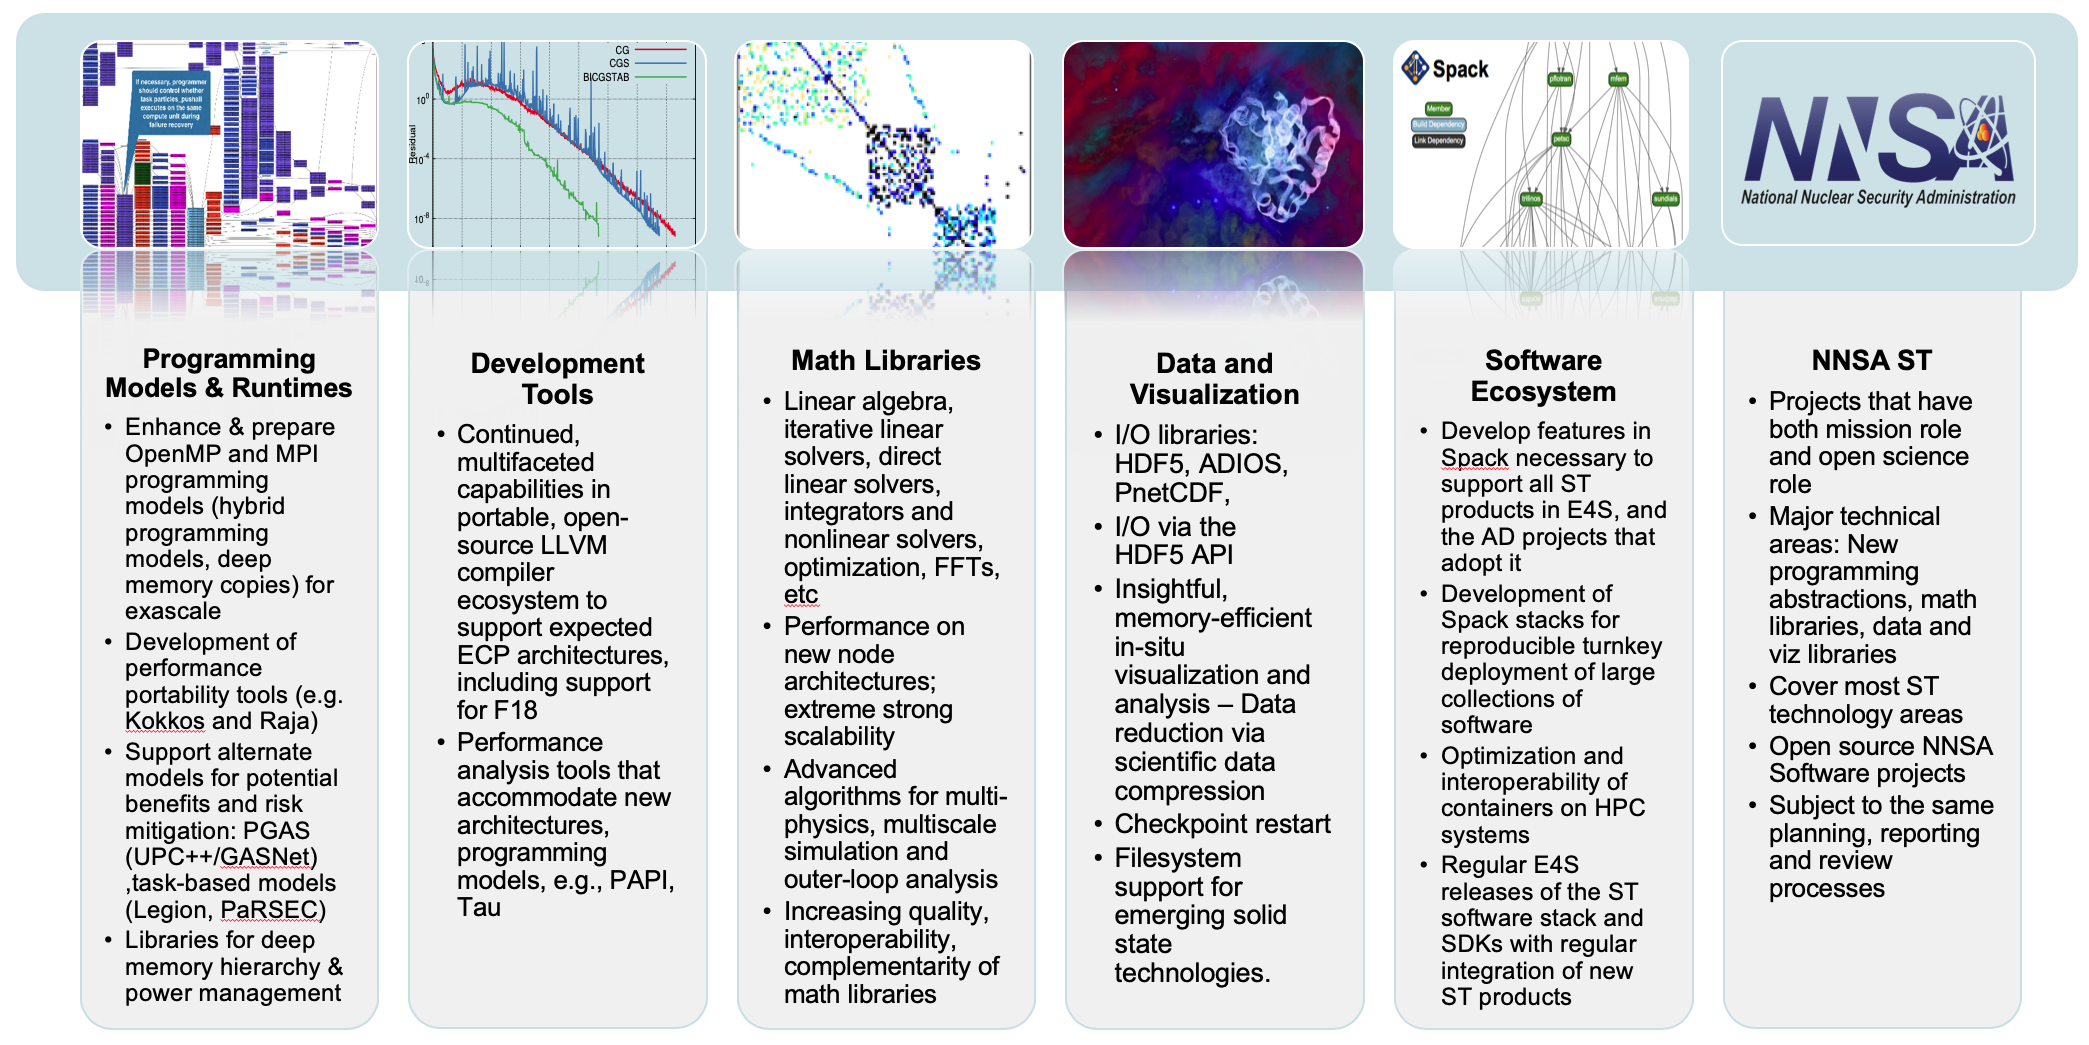
\includegraphics[width=0.9\linewidth]{L3-Overview}}
	\caption{ECP ST is composed of 6 Level-3 Technical Areas.  The first four areas are organized around functionality development themes.  The fifth is focused on technology for packaging and delivery of capabilities.  The sixth is organized around per-lab open source development at the three DOE NNSA laboratories, LANL, LLNL and SNL.  }
	\label{fig:l3-overview}
\end{figure}

\newpage
%\subsection{\pmr}
%This section presents projects in \pmr.
\subsection{\stid{1}  \pmr}\label{subsect:pmr}

\textbf{End State:} A cross-platform, production-ready programming environment that enables and accelerates the development of mission-critical software at both the node and full-system levels.

\subsubsection{Scope and Requirements}
A programming model provides the abstract design upon which developers express and coordinate the efficient parallel execution of their program. A particular model is implemented as a developer-facing interface and a supporting set of runtime layers. To successfully address the challenges of exascale computing, these software capabilities must address the challenges of programming at both the node- and full-system levels. These two targets must be coupled to support multiple complexities expected with exascale systems (e.g., locality for deep memory hierarchies, affinity for threads of execution, load balancing) and also provide a set of mechanisms for performance portability across the range of potential and final system designs. Additionally, there must be mechanisms for the interoperability and composition of multiple implementations (e.g., one at the system level and one at the node level). This must include abilities such as resource sharing for workloads that include coupled applications, supporting libraries and frameworks, and capabilities such as in situ analysis and visualization. 

Given the ECP’s timeline, the development of new programming languages and their supporting infrastructure is infeasible. We do, however, recognize that the augmentation or extension of the features of existing and widely used languages (e.g., C/C++ and Fortran) could provide solutions for simplifying certain software development activities. 

\subsubsection{Assumptions and Feasibility}
The intent of the PMR L3 is to provide a set of programming abstractions and their supporting implementations that allow programmers to select from options that meet demands for expressiveness, performance, productivity, compatibility, and portability. It is important to note that, while these goals are obviously desirable, they must be balanced with an additional awareness that today’s methods and techniques may require changes in both the application and the overall programming environment and within the supporting software stack.

\subsubsection{Objectives}
PMR provides the software infrastructure necessary to enable and accelerate the development of HPC applications that perform well and are correct and robust, while reducing the cost both for initial development and ongoing porting and maintenance. PMR activities need to reflect the requirements of increasingly complex application scenarios, usage models, and workflows, while at the same time addressing the hardware challenges of increased levels of concurrency, data locality, power, and resilience. The software environment will support programming at multiple levels of abstraction that includes both mainstream as well as alternative approaches if feasible in ECP’s timeframe. 

Both of these approaches must provide a portability path such that a single application code can run well on multiple types of systems, or multiple generations of systems, with minimal changes. The layers of the system and programming environment implementation will therefore aim to hide the differences through compilers, runtime systems, messaging standards, shared-memory standards, and programming abstractions designed to help developers map algorithms onto the underlying hardware and schedule data motion and computation with increased automation.
\subsubsection{Plan}
PMR contains nine L4 projects. To ensure relevance to DOE missions, these efforts leverage and collaborate with existing activities within the broader HPC community. The PMR area supports the research and development needed to produce exascale-ready versions of the Message Passing Interface (MPI);  Partitioned Global-Address Space Libraries (UPC++, GASNet); task-based programming models (Legion, PaRSEC); software for node-level performance portability (Kokkos, RAJA); and libraries for memory, power, and resource management.
Initial efforts focused on identifying the core capabilities needed by the selected ECP applications and components of the software stack, identifying shortcomings of current approaches, establishing performance baselines of existing implementations on available petascale and prototype systems, and the re-implementation of the lower-level capabilities of relevant libraries and frameworks. These efforts provided demonstrations of parallel performance of algorithms on pre-exascale, leadership-class machines--at first on test problems, but eventually in actual applications (in close collaboration with the AD and HI teams). Initial efforts also informed research into exascale-specific algorithms and requirements that will be implemented across the software stack. The supported projects targeted and implemented early versions of their software on CORAL, NERSC and ACES pre-exascale systems--with an ultimate target of production-ready deployment on the exascale systems.
In FY20--23, the focus will be on development and tuning for the specific architectures of the selected exascale platforms, in addition to tuning specific features that are critical to ECP applications.

Throughout the effort, the applications teams and other elements of the software stack evaluate and provide feedback on their functionality, performance, and robustness. Progress towards these goals is documented quarterly and evaluated annually (or more frequently if needed) based on PMR-centric milestones as well as joint milestone activities shared across associated software stack activities by Application Development and Hardware \& Integration focus areas.


\subsubsection{Risks and Mitigation Strategies}
The mainstream activities of ECP in the area of programming models focus on advancing the capabilities of MPI and OpenMP. Pushing them as far as possible into the exascale era is key to supporting an evolutionary path for applications. This is the primary risk mitigation approach for existing application codes. Extensions to MPI and OpenMP standards require research, and part of the efforts will focus on rolling these findings into existing standards, which takes time. To further address risks, PMR is exploring alternative approaches to mitigate the impact of potential limitations of the MPI and OpenMP programming models. 

Another risk is the failure of adoption of the software stack by the vendors, which is mitigated by the specific delivery focus in sub-element SW Ecosystem and Delivery. Past experience has shown that a combination of laboratory-supported open-source software and vendor-optimized solutions built around standard APIs that encourage innovation across multiple platforms is a viable approach and is what we are doing in PMR. We are using close interaction with the vendors early on to encourage adoption of the software stack, including well-tested practices of including support for key software products or APIs into large procurements through NRE or other contractual obligations. A mitigation strategy for this approach involves building a long-lasting open-source community around projects that are supported via laboratory and university funding. 

Creating a coordinated set of software requires strong management to ensure that duplication of effort is minimized. This is recognized by ECP management, and processes are in place to ensure collaboration is effective, shortcuts are avoided unless necessary, and an agile approach to development is instituted to prevent prototypes moving directly to product. 

\subsubsection{Future Trends}
Recently announced exascale system procurements have shown that the
trend in exascale compute-node hardware is toward heterogeneity:
Compute nodes of future systems will have a combination of regular
CPUs and accelerators (typically GPUs). Furthermore, the GPUs will not
be just from NVIDIA as on existing systems: One system will have Intel
GPUs and another will have AMD GPUs. In other words, there will be a
diversity of GPU architectures, each with their own vendor-preferred
way of programming the GPUs. An additional complication
is that although the HPC community has some experience in using NVIDIA
GPUs and the associated CUDA programming model, the community has relatively
little experience in programming Intel or AMD GPUs.  These
issues lead to challenges for application and software teams in
developing exascale software that is both portable and high performance. Below
we outline trends in programming these complex systems that will help
alleviate some of these challenges.

\paragraph{Trends in Internode Programming}
The presence of accelerator hardware on compute nodes has resulted in individual
compute nodes becoming very powerful. As a result, millions of compute
nodes are no longer needed to build an exascale system. This trend
results in a lower burden on the programming system used for internode
communication. It is widely expected that MPI will continue to serve
the purpose of internode communication on exascale systems and is the
least disruptive path for applications, most of which already use
MPI. Nonetheless, improvements are needed in the MPI Standard as well
as in MPI implementations in areas such as hybrid programming
(integration with GPUs and GPU memory, integration with the intranode
programming model), overall resilience and robustness, scalability,
low-latency communication, optimized collective algorithms, optimized support
for exascale interconnects and lower-level communication paradigms
such as OFI and UCX, and scalable process startup and management. PGAS
models, such as UPC++ and OpenSHMEM, are also available to be used by
applications that rely on them and face similar
challenges as MPI on exascale systems. These challenges are being tackled by the MPI and
UPC++/GASNet projects in the PMR area.

\paragraph{Trends in Intranode Programming}
The main challenge for exascale is in achieving performance and portability for
intranode programming, for which a variety of options
exist. Vendor-supported options include CUDA and OpenACC for NVIDIA
GPUs, SYCL/DPC++ for Intel GPUs, and HIP for AMD GPUs. OpenACC
supports accelerator programming via compiler directives. SYCL
provides a C++ abstraction on top of OpenCL, which itself is a
portable, lower-level API for programming heterogeneous
devices. Intel's DPC++ is similar to SYCL with some extensions. HIP
from AMD is similar to CUDA; in fact, AMD provides translation tools
to convert CUDA programs to HIP.

Among portable, standard programming models, OpenMP has supported
accelerators via the \texttt{target} directive starting with OpenMP version
4.0 released in July 2013. Subsequent releases of OpenMP (version 4.5
and 5.0) have further improved support for accelerators. OpenMP is
supported by vendors on all platforms and, in theory, could serve as a
portable intranode programming model for systems with
accelerators. However, in practice, a lot depends on the quality of
the implementation.

Kokkos and RAJA provide another alternative for portable,
heterogenous-node programming via C++ abstractions. They
are designed to work on complex node architectures
with multiple types of execution resources and multilevel memory
hierarchies. Many ECP applications are successfully using Kokkos and
RAJA to write portable parallel code that runs efficiently on GPUs.

We believe these options (and high-quality implementations of them) will
meet the needs of applications in the exascale timeframe. 

\newpage
\input{projects/2.3.1-PMR/2.3.1.01-PMR-SDKs/2.3.1.01-PMR-SDKs}
\newpage
\subsubsection{\stid{1.07} Exascale MPI} \label{subsubsect:mpich}
\paragraph{Overview}

MPI has been the de facto standard programming model for HPC from the
mid 90's till today, a period where supercomputing performance
increased by six orders of magnitude.  The vast majority of DOE's
parallel scientific applications running on the largest HPC systems
use MPI. These application codes represent billions of dollars of
investment. Therefore, MPI must evolve to run as efficiently as
possible on Exascale systems. Our group at Argonne developed a
high-performance, production-quality MPI implementation, called MPICH.
The focus areas of the Exascale MPI / MPICH project are: (1)
continuous improvement of the performance and capabilities of the
MPICH software to meet the demands of ECP and other broader DOE
applications, (2) coordinate vendor and supercomputing center
interactions to ensure efficient solutions to applications, and (3) be
involved in the MPI forum and standardization efforts to ensure
continuity of the work beyond this project.

MPICH team is involved in the formation of the MPI Forum and have been
deeply involved in defining the MPI standard since 1992. MPICH has
helped prototype and define the majority of the features in the MPI
standard. As such, MPICH has been one of the most influential pieces of
software in accelerating the adoption of the MPI standard by the HPC
community. MPICH has been adopted by leading vendors into their own
derivative implementations. Examples include Intel (for Intel MPI), Cray
(for Cray MPI), IBM (for IBM PE MPI), Mellanox (for MLNX-MPI), Microsoft
(for MS-MPI), and Ohio State University (for MVAPICH). MPICH and its
derivatives are exclusively used in 7 of the top 10 supercomputers in
the world today. MPICH is the recipient of a number of awards including
an R\&D 100 award.

\paragraph{Key Challenges}

While we believe MPI is a viable programming model at Exascale, both
the MPI standard and MPI implementations have to address the
challenges posed by the increased scale, performance characteristics
and evolving architectural features expected in Exascale systems, as
well as the capabilities and requirements of applications targeted at
these systems. The key challenges are:

\begin{enumerate}

\item Interoperability with intranode programming models having a high
  thread count~\cite{Hybrid1, Hybrid2, FT2} (such as OpenMP,
  OpenACC and emerging asynchronous task models);

\item Scalability and performance over complex
  architectures~\cite{Perf1, Perf2, FT2, Perf4} (including high core
  counts, processor heterogeneity and heterogeneous memory);

\item Software overheads that are exacerbated by lightweight cores and
  low-latency networks;

\item Enhanced functionality (extensions to the MPI standard) based on
  experience with applications and high-level libraries/frameworks
  targeted at Exascale; and

\item Topics that become more significant as we move to the next
  generation of HPC architectures: memory usage, power, and
  resilience.

\end{enumerate}

\paragraph{Solution Strategy}

The Exascale MPI project has the following primary technical thrusts:
(1) \textbf{Performance and Scalability} (2) \textbf{Heterogeneity}
(3) \textbf{Topology Awareness} (4) \textbf{Fault Tolerance} and (5)
\textbf{MPI+X Hybrid Programming}.

Our solution strategy started by addressing performance and
scalability aspects in MPICH related to network address
management~\cite{memscal}.  Apart from this, we also looked at
communication strategies which allow the MPI library to be as
lightweight as possible~\cite{ch41, ch42}. Other solutions include
investigation and evaluation of communication relaxation hints,
investigation of optimizations to memory scalability in MPICH and
improvements to MPI RMA operations.

Exascale MPI heterogeneity efforts~\cite{Hetero1, Hetero2, Hetero3}
started with the survey on heterogeneous memory architectures on
upcoming DOE machines and how MPICH can take advantage of
them~\cite{hexe}. The efforts also included the investigation of
utilizing heterogeneous memory inside the MPI implementation and
evaluation of applications~\cite{hetero4}. The heterogeneity efforts
further extended to investigating and developing technologies for GPU
integration for the better support of the coming Exascale
supercomputers.

Exascale MPI topology awareness efforts~\cite{Topo1,Topo2} originated
with the investigation and evaluation of hints based on topology
awareness and optimizations to virtual topology functionality in
MPICH~\cite{topo-io,topo-io2}. The other efforts include investigation
of topology-aware collectives and neighborhood collectives in
MPICH~\cite{coll} and evaluation of the selected ECP applications.

Exascale MPI fault tolerance efforts~\cite{FT1, FT2} started with
support for handling noncatastrophic errors in MPI. The second effort
included defining the scope of errors in MPI, a prerequisite for
user-level failure mitigation. Other efforts in this direction
includes standardizing these efforts in MPI and evaluating application
suitability for fault tolerance.

Exascale MPI+X hybrid programming developed firstly with effort in
improving interoperation of MPICH with threads~\cite{interthread}.
Secondly, we developed the work-queue data transfer model for
multithreaded MPI communication~\cite{workq}. We have included support
for interaction of MPICH with user-level thread (ULT)
libraries~\cite{ULT}, primarily targeting Argobots and the BOLT
runtime~\cite{BOLT}.  Other issues that are being looked at include the
investigation and evaluation on multiple virtual communication
interfaces for multithreaded MPI communication~\cite{VCI}.

\paragraph{Recent Progress}

The recent release of MPICH 3.4b1 version includes deliverables from the
major milestones of FY2020. Figure~\ref{fig:fy20} provides the details
of them. In the first milestone, we created the collective algorithm
selection framework which allows MPI to choose different algorithm for
collectives operations based on multiple factors including number of
processes, network topology and support of hardware acceleration. The
user of MPICH can provide a configuration file to describe the criteria
for choosing different collective algorithms. We expect the vendors
utilizing this capability to provide collective selection strategies
that is optimized for the target supercomputers. The end-user could also
generate their own strategies that is fine-tuned to the characteristic
and needs of their applications.
In the second milestone, we added the support for GPU in MPI
communication. This allows a buffer in the GPU memory to be used
directly in MPI communication operations. MPICH's GPU support can
utilize the native support of fast GPU communication in hardware while also
provide a fallback mode for more complex MPI communication pattens. We
also created a new high-performance datatype engine that further
utilizes GPU for handling non-contiguous datatype in MPI communication.

Lastly, we made many efforts in participating the standardization of
MPI-4 by discussing proposed features and contributing the feedback for
our users back to the MPI forum. This has led to several new features
being accepted by the MPI Forum.

\begin{figure}[htb]
  \centering
  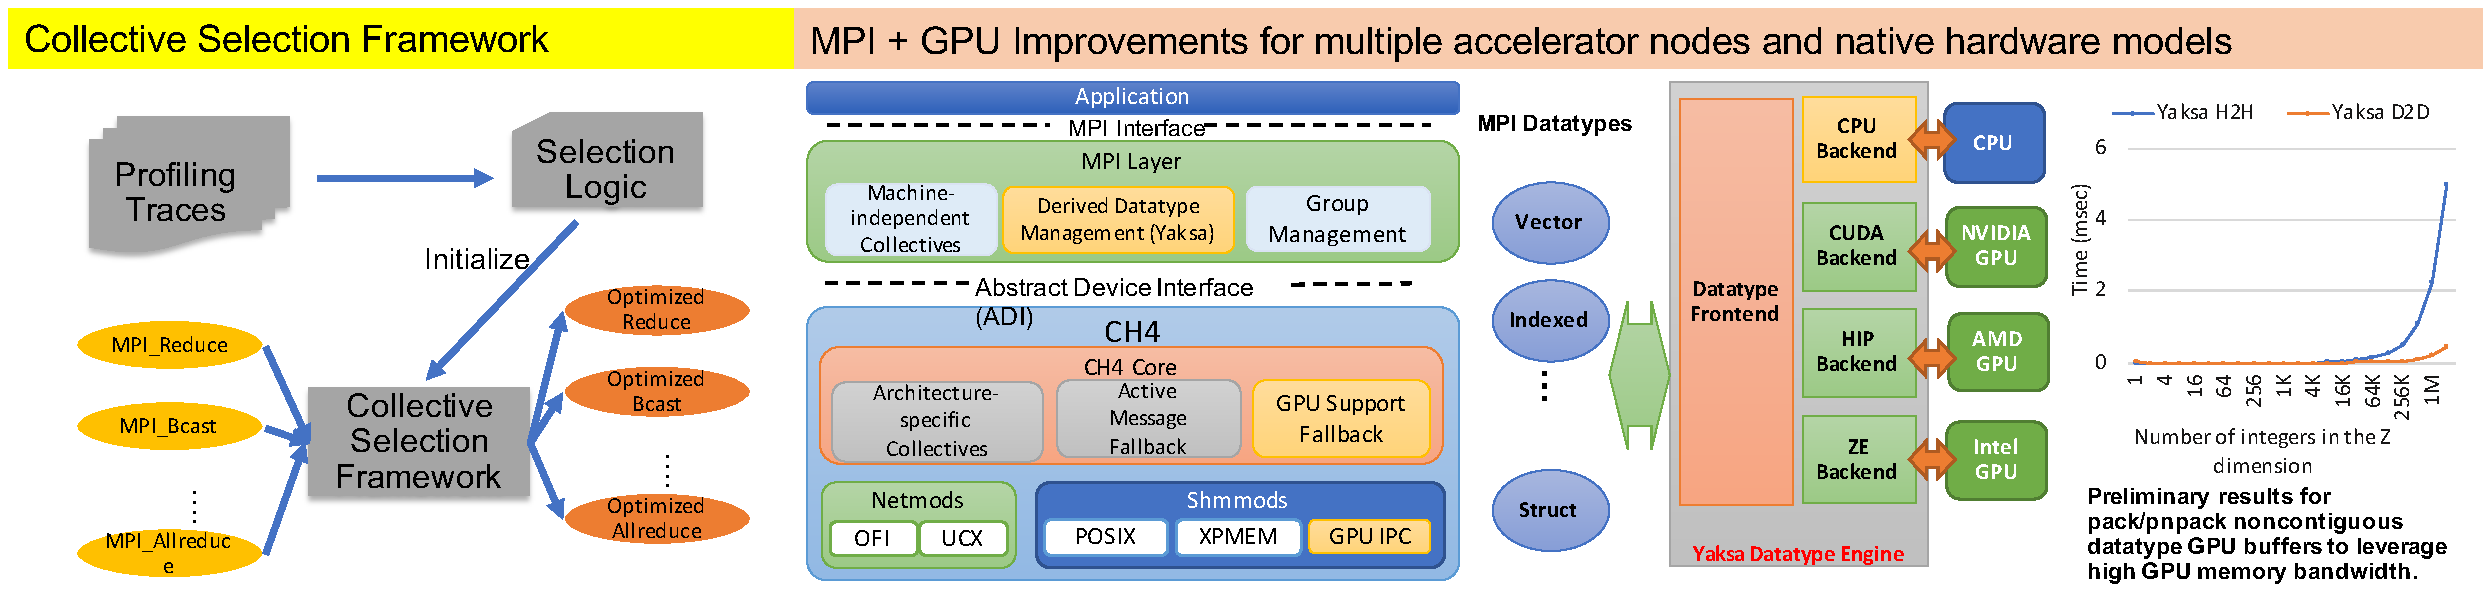
\includegraphics[width=6in]{projects/2.3.1-PMR/2.3.1.07-Exascale-MPI/MPICH-recent-milestones.pdf}
  \caption{\label{fig:fy20}Major MPICH milestones completed in fiscal year 2020}
\end{figure}

\paragraph{Next Steps}
A major focus of the ongoing Exascale MPI efforts is further
improvements to the MPI+GPU support. This includes support for GPU
stream triggered MPI operations, optimized support for noncontiguous
data and software evaluations. Another focus of FY2021 is the
implementation of new features in MPI-4 standard including persistent
collective operations. We will also make effort for improving the MPICH
testing infrastructure by improving the testsuite and promoting
integration ECP systems to provide better test coverage and a
close-to-production test environment. This would enhance the readiness
of MPICH for exascale systems.

\newpage
\subsubsection{\stid{1.08} Legion}

\paragraph{Overview}
This project focuses on the development, hardening and support of the
Legion Programming System (\url{https://legion.stanford.edu}) with a
focus on Exascale platforms and workloads that can benefit from
Legion's features.  At a fundamental level our focus is on the key
capabilities (e.g. correctness, performance, scalability) of an
alternative programming model for ECP that seeks to expose additional
levels of parallelism in applications.  In addition, Legion also
enables a separation of concerns of the implementation of an
application from how it is mapped onto a given system architecture.

Our efforts are currently focused on addressing bugs, refactoring the
implementation for improved stability, performance and scaling,
extending support for the selected exascale platforms (Aurora and
Frontier), and also expanding the feature set as needed for both
application and platform nuances.

The Legion Programming System is freely available with an Apache-based
open source license and is hosted at GitLab:

\begin{quote} 
  \url{https://gitlab.com/StanfordLegion/legion}
\end{quote}

\paragraph{Key Challenges}
While Legion addresses a number of key challenges in improving system
utilization, some aspects of platform portability, and is becoming
more widely used, it is still a new programming system and therefore
there is a cost to rewriting applications.  This aspect makes
significant adoption a risk within ECP and additional effort is being
taken to improve stability and find unique use cases.  aspects of performance and scaling to
match aspects of more mature technologies.

We have focused much of our efforts on emerging use cases that are
related to machine learning and data-centric workloads.  These domains
are much easier to have a substantial impact as the application codes
rely on external tools (e.g. TensorFlow, Python, etc.) vs. years of
established code written in MPI and/or OpenMP.  We are already seeing
clear benefits of focusing our efforts in this direction. This has
helped us to increase our overall impact as well focus on areas of
adoption across more specialized application needs in support of
machine learning and other data-centric workloads.

\paragraph{Solution Strategy}
As a collaboration between Los Alamos, Stanford University and R\&D
efforts at NVIDIA, SLAC, Facebook, MIT, and others.  We are providing
the overarching implementation of Legion that captures the most stable
(correct and feature complete) version of the programming system.  In
addition, we are actively looking for opportunities to educate the
community about Legion and other data-centric and task-based
approaches to programming.

We have continued working with ExaFEL (AD 2.2.4.05) and the CANDLE
project (AD 2.2.4.03) to provide support for Legion.  We also provide
support and software releases related to the efforts going on within
LANL's ATDM Programming Models and Runtimes project (part of ST
2.3.6.01), that refine, identify needs and requirements that are in
support of Ristra (LANL's National Security application AD 2.2.5.01).
Our project includes management of the current repository and
quarterly, or more frequent, releases of Legion to the broader
community.  We are also supporting approaches that support Legion
inter-operation with other languages and programming systems --
e.g. MPI, OpenMP, Kokkos, Fortran, Python.

We have continued our work on improving performance and scaling of
training deep learning applications.  In particular, we are working
closely with CANDLE's requirements for ML training and inference on
large DNNs. Our most recent progress is discussed below. 

\paragraph{Recent Progress}

We continue to discover and address both performance and scalability
issues in the runtime.  In addition, for use cases within ECP, and
also a growing set of users outside of ECP, we have continued to
identify and address bugs and other issues (e.g. missing features).

As mentioned above, our we continue to focus on improving training
times for CANDLE's DNN use cases and also improving developer productivity
when using Flexflow (the DNN training layer built on top of Legion).  
We are specifically working to make sure the feature set of FlexFlow system
provides the necessary functionality and as part of this we have recently
completed a Python layer for FlexFlow that provides support for the Keras
(TensorFlow) interface.  This allows TensorFlow programs to be run using
FlexFlow with very minimal changes to the original Python code.  FlexFlow
is now available as open source under an Apache License:

\begin{quote} 
  \url{https://github.com/flexflow/FlexFlow} 
\end{quote}

We are now starting work on new training networks with CANDLE and also
working on providing a PyTorch compatibility interface to provide the same
ability to run widely used Python applications for machine learning using
Flow and Legion as the underlying runtime systems. 

Finally, we currently have a start on supporting both AMD and Intel
GPUs.  After AMD deprecated the CUDA Driver API in their HIP software
layer we had to rewrite a portion of the underlying implementation to
re-establish AMD support.  This initial work is complete and Legion
applications are running successfully on currently available AMD GPUs.
Similar efforts are underway for Intel systems using the oneAPI
interface.  The initial implementation has run into a few issues
within Intel's software stack that we are waiting to be resolved.  We
are on target to successfully run on Intel's stack by late in 2020 or
early 2021.  We have also completed an additional lower-level
MPI-based transport layer underneath Legion to provide a level of risk
mitigation at the lower levels of the Legion runtime (Realm).

\paragraph{Next Steps}

Our plans for the next year are to continue focusing on the challenges
presented by the upcoming exasacle system architectures and on
hardening and improving the overall performance and scalability of
Legion.  These efforts will specifically begin to focus on AMD and
Intel hardware with an eye towards performance at the node level
(limited by the availability and stability of appropriate hardware
resources).

We will continue to work on the Python interfaces for Legion with a
focus on the Keras and PyTorch features requested by CANDLE.  This
will include seeking out and improving our outreach.  Our regular open
source releases of Legion and FlexFlow will continue.  Further work will
need to be done to focus on bug fixes, improving capabilities, improving
developer productivity, and addressing performance issues on both existing
and upcoming platforms.




\newpage
\subsubsection{\stid{1.09} Distributed Tasking at Exascale: PaRSEC}


\paragraph{Overview}

The PaRSEC Environment provides a software ecosystem composed of a runtime
component to dynamically execute task-based applications on heterogeneous
distributed systems, and a productivity toolbox that comprises a development
framework for the support of multiple Domain Specific Languages (DSLs) and
extensions, with debugging, trace collection, and analysis tools.
%
The PaRSEC project team is dedicated to solving two challenging and
interdependent problems facing the ECP developer community: First, how to create
an execution model that enables developers to express as much parallelism as
possible in their applications, so that applications effectively utilize the
massive collection of heterogeneous devices ECP machines will deploy. Second,
how to ensure the execution model is flexible and portable enough to actually
provide and sustain a performance benefit by increasing the scientific
productivity of the application developers, not only for the ECP target
environments but for the foreseeable future.

\begin{wrapfigure}[17]{l}{.45\linewidth}
\includegraphics[scale=0.3]{projects/2.3.1-PMR/2.3.1.09-ParSEC/PaRSEC-diagram.png}
\caption{PaRSEC architecture\label{fig:parsec} based on a modular framework where each
component can be dynamically activated as needed.}
\end{wrapfigure}
%
PaRSEC is an open source, community-based implementation of a generic task-based
runtime that is freely available, and used by an increasing number of software
libraries.
%  The PARSEC development team is mainly comprised of research staff at % UTK,
%  but regular contributions from the community are provided via our presence %
%  on GitHub and Bitbucket.
The project focuses on providing a stable and efficient infrastructure for quick
prototyping of different approaches to define task-based languages able to
exploit the full range of capabilities of Exascale platforms. Without such a
project, and based on the current state of task-based runtimes, potential users
will be stuck either in fixed programming paradigms, or with a particular,
potentially less efficient, mix of programming languages. The DTE project
provides means to maintain a high competitiveness in the field leading to more
innovation on addressing the challenges we are facing toward scalable,
efficient and Exascale-ready programming paradigms.

\paragraph{Key Challenges}
%\textit{Describe what is hard to do, why it is challenging.}

As Exascale platforms delivery become a closer deadline, a increasing number of
aspects of the hardware and software environment still pose challenges. First
and foremost, keeping pace with the architectural changes on current and future
platforms requires changes not only on how we take advantage of the hardware
capabilities, but how we reshape our algorithms and applications to expose
enough parallelism to maximize the use of the underlying hardware. The number of
nodes, threads per node, memory hierarchies and support for increased
computational capabilities (accelerators) will continue to increase, while the
currently available programming paradigms are still struggling with parallelism
at the node level.

\paragraph{Solution Strategy}
%\textit{Describe your basic strategy for addressing the challenges.}
The approach followed in PaRSEC is to provide a low-level, flexible and dynamic
runtime able not only to schedule tasks at the node level, but to handle data
transfers between different memory (both inter- and intra-nodes), memory
hierarchies, heterogeneous architectures with support for accelerators with a
simple programming scheme. The proposed approach envisions a middle-ground
solution, addressing both hardware and software challenges. At the hardware
level a team of dedicated developers extends PaRSEC to map it's capabilities to
the hardware and to improve it's scalability and performance. At the upper
software level the runtime interactions are through Domain Specific Languages
with the target domain scientists in mind, that will facilitate the expression
of algorithmic parallelism with familiar constructs mapped on the exposed
low-level capabilities. To facilitate the integration of PaRSEC-driven libraries
into larger and complex applications, PaRSEC natively interoperate with other
programming paradigms, including some target of the ECP PMR support, such as
PGAS, MPI, OpenMP and Kokkos. This integration provides a smooth transition for
library developers that embrace the PaRSEC runtime, providing a platform where a
shift to a new programming paradigms can be done in stages of increased
complexity~\cite{lorapo-protools,BLR_LU,parsec_pdgemm}.
% In this model, PaRSEC remains in full control of data tracking and
% allocation on the managed accelerator.

\paragraph{Recent Progress}

The software release (2020.10) provides many new additions to the low-level task
runtime, supports for a number of hardware capabilities (multi-stream GPU, NVLink,
P9 atomic ops, ARM SVE support), brings significant improvements to the performance
and scalability of the runtime, and addresses many pending issues.
%
% The installation system has been improved to take advantage of the latest
% capability of CMake, and scripts for seamless integration in the ECP software
% ecosystem (via SPack). Significant improvements have also been added on the
% performance and scalability of the runtime, as shown by the results below.
%
On the software quality side, the PaRSEC runtime has been evaluated and amended
to compile and run on all pre-Exascale platforms (ALCF Mira, Theta; OLCF
Summit), as well as some early platforms based on the new ARM architecture.
PaRSEC now includes a Spack definition file to ease the deployment on
future target systems as part of the system software xSDK effort.

%
% Recent work: irregular block-sparse GEMM on Summit
%

\begin{wrapfigure}{l}{.45\linewidth}
\centering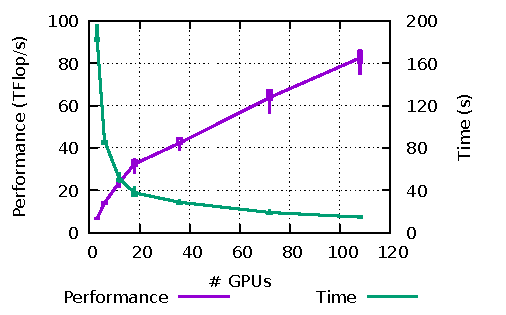
\includegraphics[width=.9\linewidth]{projects/2.3.1-PMR/2.3.1.09-ParSEC/irr-bs-gemm-combined.pdf}
\caption{Time to solution and Performance as a function of the number
  of V100 GPUs on Summit, for the molecule
  $C_{65}H_{132}$\label{fig:irrbsgemm}}
\end{wrapfigure}
The PaRSEC team, in collaboration with NWChemEx project researchers,
developed an efficient and portable tensor product algorithm
specifically designed for the computational chemistry domain needs on
top of the PaRSEC runtime. This includes an efficient matrix product
operation for hybrid architectures, like Summit, with an irregularly
blocked, block-sparse representation of matrices. Moreover, the
requirements on this implementation were extremely strict, the
matrices are rectangular and extremely large in at least one of their
dimensions, such that none of the input matrices could fit in the
aggregated memory of all GPUs. The algorithm and a deeper analysis of
the results are described in~\cite{parsec::rr::irrbs}.

Figure~\ref{fig:irrbsgemm} shows a strong scaling performance
evaluation of this algorithm, when applied to the main tensor product
required by the CCSD method to simulate the electronic structure from
first principles. The simulated molecule was $C_{65}H_{132}$, which is
a quasi-1-dimensional system and small atomic orbital basis, where the
sparsity of tensors is maximized while the optimal (from the data
compression perspective) tile size is small. That molecule is
representative of applications to 1-d polymers and quasi-linear
molecules (such as some proteins), while the choice of the atomic
orbital basis is representative of medium-precision simulations in
chemistry and condensed phase. Such use case stresses the system and
algorithm as it implies a significant sparsity: the largest matrix,
while being of square of rank $2,464,900$, has only a density of
3.1\%.

The strong scaling evaluation shows a parallel efficiency of 35\%,
with a time to solution at 180s on 3 GPUs, going down to 13s at 118
GPUs.
% The performance per GPU decreases with the number of nodes,
% between 36\% at 3 GPUs and 12\% at 118 GPUs.
Compared to the state of the art, DBCSR~\cite{parsec::dbcsr} can only
run problems that fit in the GPU memory, preventing us to run the same
experiment, but experiments on synthetic problems that fit in memory
show an improvement by a factor two, while
TiledArray~\cite{parsec::tiledarray} cannot leverage the GPUs of
Summit without using PaRSEC and would run, on the CPUs of Summit ten
times slower.
%
% End
%

\begin{wrapfigure}[16]{l}{.45\linewidth}
\vspace*{-1em}\centering\includegraphics[scale=0.50]{projects/2.3.1-PMR/2.3.1.09-ParSEC/slate_updated_nacl.pdf}
  \caption{Comparison of DPLASMA and SLATE Cholesky factorization over PaRSEC with
           SLATE and ScaLAPACK on 64 nodes 12 cores each\label{fig:slate-parsec}}
\end{wrapfigure}
An important aspect of the DTE project is to define and prototype scalable
domain specific languages that enable a productive expression of parallelism for
end-user communities. PaRSEC presents multiple programming interfaces
(Parameterized Task Graphs for maximum parallelism, the popular serial task
insertion dataflow model to provide direct access to the runtime). In addition
the DTE team is in close contact with application teams to define parallel
abstractions that are suitable for their domain usage. Notably, the PaRSEC team
has ongoing collaboration with the SLATE linear algebra package and NWChemEx and
GAMESS chemistry package teams.

In this context it is interesting to highlight the first step toward
the integration of the PaRSEC framework into the SLATE (2.3.3.09) in
the context of the shared milestone (STPM11-23). The first prototype
of the application ran in a distributed environment and showed the
capability of the SLATE library using a modern fully capable runtime
system. This work involved enhancing the insert task interface
available in the ParSEC runtime to map onto the logic of a SLATE
algorithm.

Figure~\ref{fig:slate-parsec} compares different implementation of the
Cholesky factorization. On one side we have two reference
implementation for distributed linear algebra, ScaLAPACK and the
current version of the SLATE library (using OpenMP for intra-node
parallelism and MPI for communications). On the other side we have two
DSL expressing the same algorithm but using PaRSEC as the underlying
runtime, the Dynamic Task Discovery (DTD) an approach similar to
OpenMP but working on a distributed setting, and a version of the
SLATE library where instead of relying on explicit parallelism
(OpenMP) and communications (MPI) it rely on implicit dependencies
qmanagement via PaRSEC.


% side including the integration of SLATE and PaRSEC. Two domain
% specific languages that have the capability to do linear algebra; then
% against the regular SLATE using OpenMP for intra-node parallelism, and
% MPI for communication; and finally against ScaLAPACK, which is the
% reference for distributed linear algebra.

%
% Recent work: ScaLAPACK - DPLASMA - PaRSEC
%


%\begin{wrapfigure}{l}{.42\linewidth}
%\centering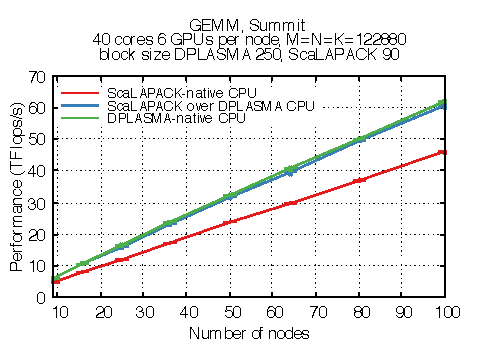
\includegraphics[width=.9\linewidth]{projects/2.3.1-PMR/2.3.1.09-ParSEC/scalapack_cpu_GEMM.pdf}
%\centering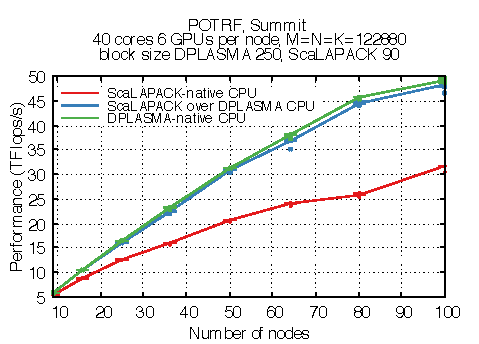
\includegraphics[width=.9\linewidth]{projects/2.3.1-PMR/2.3.1.09-ParSEC/scalapack_cpu_POTRF.pdf}
%\caption{Performance using only CPUs of native ScaLAPACK, ScaLAPACK
%  over DPLASMA and native DPLASMA for GEMM and
%  POTRF.\label{fig:scalapack_cpu}}
%\end{wrapfigure}
%\begin{wrapfigure}{l}{.42\linewidth}
%\centering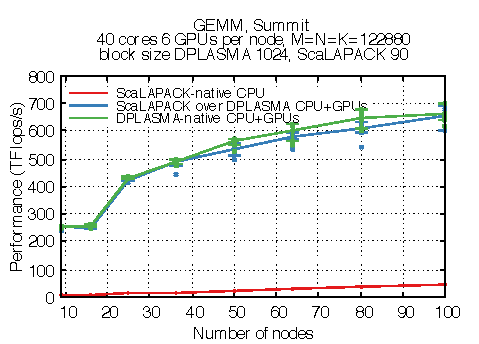
\includegraphics[width=.9\linewidth]{projects/2.3.1-PMR/2.3.1.09-ParSEC/scalapack_gpu_GEMM.pdf}
%\centering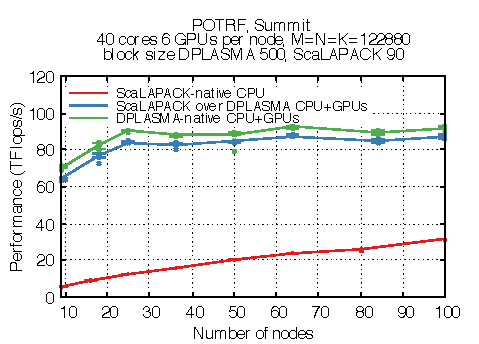
\includegraphics[width=.9\linewidth]{projects/2.3.1-PMR/2.3.1.09-ParSEC/scalapack_gpu_POTRF.pdf}
%\caption{Performance using GPUs of native ScaLAPACK, ScaLAPACK over
%  DPLASMA and native DPLASMA for GEMM and
%  POTRF.\label{fig:scalapack_gpu}}
%\end{wrapfigure}
\begin{wrapfigure}{l}{.45\linewidth}
\centering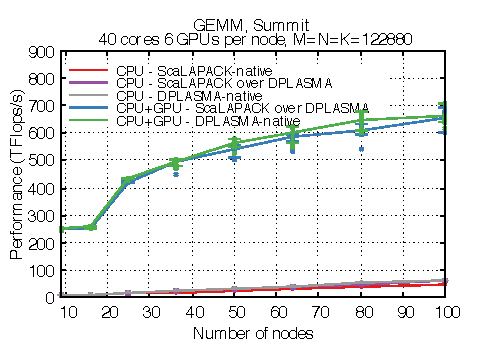
\includegraphics[width=.9\linewidth]{projects/2.3.1-PMR/2.3.1.09-ParSEC/scalapack_GEMM.pdf}
\centering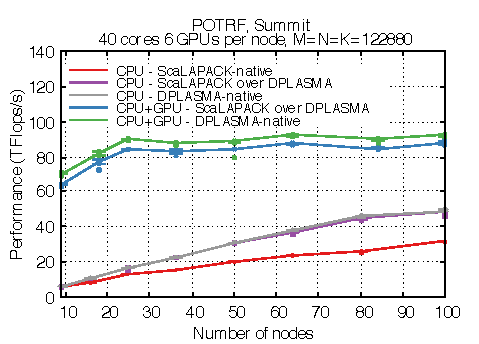
\includegraphics[width=.9\linewidth]{projects/2.3.1-PMR/2.3.1.09-ParSEC/scalapack_POTRF.pdf}
\caption{Performance using GPUs of native ScaLAPACK, ScaLAPACK over
  DPLASMA and native DPLASMA for GEMM and
  POTRF.\label{fig:scalapack_gpu}}
\end{wrapfigure}
In the context of milestone STPM11-81, the PaRSEC team worked to
enable the usage DPLASMA as a replacement for ScaLAPACK.  This
functionality is provided as an independent library which contains a
wrapped version of the ScaLAPACK API and hides the PaRSEC API from the
application while it constructs the structures necessary for the
operation with matrices represented on ScaLAPACK memory layout.  Users
of applications exploiting ScaLAPACK can link against this independent
library to run the wrapped routines over DPLASMA-PaRSEC, while any
other ScaLAPACK function, i.e. that does not have an equivalent
provided by DPLASMA, will use the original ScaLAPACK implementation.
This approach reduces to a minimum the changes that need to be
performed on the ScaLAPACK application, while enabling the
exploitation of the algorithms implemented on DPLASMA and the
operation over PaRSEC for a better exploitation of the available
hardware resources.


Figure~\ref{fig:scalapack_gpu} compare the
performance of the ScaLAPACK wrapper extensions against the native
DPLASMA and native ScaLAPACK in their typical usage scenarios (one
process per core for ScaLAPACK),
% Experiments were run using a dense matrix with dimensions 122~880 in
% double precision. The internal block size and the process grid have
% been tuned for the best performance on each library. In all cases,
% the native ScaLAPACK tests were ran spawning one process per core
while DPLASMA tests (native DPLASMA and ScaLAPACK over DPLASMA) use
one thread per core and one process per node on the experiments using
only the CPU and two processes per node, each exploiting 3 GPUs, are
used on the GPU tests.
%
In all cases, the performance achieved by running ScaLAPACK over
DPLASMA is more than 90\% the performance of native DPLASMA.  For the
CPU-only experiments, the usage of the DPLASMA wrapper introduces an
speedup of 1.73x for GEMM (minimum 1.64x, maximum 1.88x) and 1.49x for
POTRF (minimum 1.27x, maximum 1.71x) .  When exploiting also the GPUs
of the computation nodes, the performance is increased by 16.75x for
GEMM (minimum 10.79x, maximum 25.68x) and by 4.27x for POTRF (minimum
2.77x, maximum 6.70x).  The lower performance of the DPLASMA's POTRF
over GPUs is explained because in the current implementation of this
algorithm not all the tasks are run on GPUs. However, further
improvements of DPLASMA algorithms that will be integrated in the next
release of DPLASMA will likely achieved similar performance when used
for wrapping the ScaLAPACK routines. Therefore, enabling applications
already using the ScaLAPACK API to improve their usage of the
available hardware resource with very little effort that is translated
in important performance benefits.

%
% End
%

\paragraph{Next Steps}
%\textit{Describe what you are working on next.}
% Improve DTE accelerator support and interoperability with other
% programming models
To provide programmers with more supervision over how accelerators are
integrated and used by the runtime, a need to provide finer control of the
resource usage by the runtime system has arisen. We are developing new APIs to
allow the programmers to advise the runtime system with respect to data
placement, prefetching, and management of cache.
%
Programming interoperability should not be limited to node-level programming
models but should extend to distributed programming. Execution modes where part
of the application is expressed in native MPI (including communicating tasks)
and other parts using PaRSEC DSLs, running above the task system in a tightly
coupled manner, are being developed.

% Facilitate DSL integration

% Provide better libraries and tools integration
The set of tools that come with the PaRSEC runtime environment to
assess performance, find bottlenecks, improve scheduling and debug the
task-based application are being improved to expose the information
in a format compatible with TAU, Score-P and other
tools that are already familiar to ECP users.

\newpage
\subsubsection{\stid{1.14} GASNet-EX}\label{subsubsect:gasnet-ex}
\paragraph{Overview} 

The Lightweight Communication and Global Address Space Support project (Pagoda)
is developing GASNet-EX~\cite{gasnet-site}, a portable high-performance communication layer
supporting multiple implementations of the Partitioned Global Address Space
(PGAS) model.
GASNet-EX clients include Pagoda's PGAS programming interface UPC++~\cite{upcxx-ipdps19,upcxx-site}
 and the Legion Programming
System~\cite{bauer2012legion,legion-site} (WBS~2.3.1.08).

GASNet-EX's low-overhead communication mechanisms are designed to maximize
injection rate and network utilization, tolerate latency through
overlap, streamline unpredictable communication events, minimize
synchronization,
leverage hardware support for communication involving accelerator memory,
and efficiently support small- to medium-sized
messages arising in ECP applications.  GASNet-EX enables the ECP
software stack to exploit the best-available communication mechanisms,
including novel features still under development by vendors.  The
GASNet-EX communications library and the PGAS models built upon it
offer a complementary, yet interoperable, approach to ``MPI + X'',
enabling developers to focus their effort on optimizing
performance-critical communication.

We are co-designing GASNet-EX with the UPC++ development team with
additional input from the Legion and
(non-ECP) Cray Chapel~\cite{chapel-chapter,chapel-site} projects.

\paragraph{Key  Challenges}

Exascale systems will deliver exponential growth in on-chip parallelism and
reduced memory capacity per core, 
increasing the importance of strong
scaling and finer-grained communication events.  
The pervasive use of accelerators introduces heterogeneous systems in which
the engines providing the majority of the compute capability are not well
suited to other tasks.
Success at exascale demands that
software minimize the overheads incurred upon lightweight cores and accelerators,
especially avoiding long, branchy serial code paths; 
this motivates a requirement for efficient
fine-grained communication.
These problems are exacerbated by application trends; many of the ECP applications require
adaptive meshes, sparse matrices,
or dynamic load balancing.
All of these characteristics favor the use of
low-overhead communication mechanisms that
can maximize injection rate and network utilization, tolerate latency through
overlap, accommodate unpredictable communication events, minimize synchronization,
leverage hardware support for communication involving accelerator memory,
and efficiently support small- to medium-sized messages. The ECP software stack
needs to expose the best-available communication mechanisms, including novel
features being developed by the vendor community.

\paragraph{Solution Strategy}

The PGAS model is a powerful means of addressing these
challenges and is critical in building other ECP programming systems,
libraries, and applications.  We use the term {\em PGAS} for models that support
one-sided communication, 
including contiguous and non-contiguous remote memory access (RMA) operations such as put/get
and atomic updates. Some of these models also include support for remote function invocation.
GASNet-EX~\cite{gasnet-lcpc18} is a communications library that provides the foundation for implementing
PGAS models, and is the successor to the widely-deployed GASNet library.
We are building on over 15 years of experience with the GASNet~\cite{gasnet-site,gasnet-spec}
communication layer to provide production-quality implementations that include
improvements motivated by
technology trends and application experience.  

The goal of the GASNet-EX team is to provide a portable, high-performance PGAS
communication layer for exascale and pre-exascale systems, addressing the challenges
identified above.
GASNet-EX provides interfaces that efficiently match the RDMA capabilities of modern
inter-node network hardware and intra-node communication between distinct address spaces.
New interfaces for atomics and collectives have enabled offload to current
and future network hardware with corresponding capabilities.
These design choices and their implementations supply the low-overhead communication
mechanisms required to address the requirements of exascale applications.

\begin{figure}[htb]
  \centering
  \subfloat[8-byte RMA Latencies\label{fig:rma-lat-bars}]{
     \includegraphics[width=0.432\textwidth]{projects/2.3.1-PMR/2.3.1.14-UPCxx-GASNet/latency_bars.pdf}
  }
  \subfloat[Summit Flood Bandwidth\label{fig:summit-bw}]{
     \includegraphics[width=0.504\textwidth]{projects/2.3.1-PMR/2.3.1.14-UPCxx-GASNet/Summit-slide-BW.pdf}
  }
  \caption{\label{fig:gasnet-ex-rma} Selected GASNet-EX vs. MPI RMA Performance Results}
\end{figure}

Figure~\ref{fig:gasnet-ex-rma} shows representative results from a
paper~\cite{gasnet-lcpc18} comparing
the RMA performance of GASNet-EX against MPI on multiple systems including
NERSC's Cori and OLCF's Summit%
\footnote{The paper's results from Summitdev
have been replaced by more recent (June 2019) results from OLCF's newer Summit system.}.
These results demonstrate the ability of a PGAS-centric runtime to
deliver performance as good as MPI, and often better.
%
The paper presents experimental methodology and system descriptions, which are
also available online~\cite{gasnet-site}, along with results for additional
systems.

Figure~\ref{fig:rma-lat-bars} shows the latency of 8-byte RMA Put and Get operations on
four systems, including two distinct network types and three distinct MPI
implementations.
%
GASNet-EX's latency is 6\% to 55\% better than MPI's on Put and 5\% to 45\%
better on Get.
%
Algorithms sensitive to small-transfer latency may become practical in PGAS
programming models due to these improvements relative to MPI.

Figure~\ref{fig:summit-bw} shows flood bandwidth of RMA Put and Get over the
dual-rail InfiniBand network of OLCF's Summit.
GASNet-EX's bandwidth is seen to rise to saturation at smaller
transfer sizes than IBM Spectrum MPI, with the most pronounced differences
appearing between 4KiB and 32KiB.
%
Comparison to the bandwidth of MPI message-passing (dashed green series) illustrates the
benefits of one-sided communication, a major feature of PGAS models.


\paragraph{Recent Progress}

The most notable work on GASNet-EX in the past year has been in two areas:

\textbf{Device (GPU) Memory Support}.
``Memory kinds'' is the GASNet-EX term for support for communication involving
memory other than host memory, and in the context of ECP refers primarily to
accelerator devices such GPUs.
The GASNet-EX APIs for memory kinds have been co-designed with the developers
of UPC++ and the Realm runtime layer of the Legion Programming System
(WBS~2.3.1.08).  
Starting in October 2020, GASNet-EX can now leverage the GPUDirect RDMA (GDR)
capabilities of modern NVIDIA GPUs and Mellanox network adapters (such as those
on Summit) to perform one-sided RMA involving GPU memory without
the overheads of staging through intermediate buffers in host memory.

\textbf{Scalability}.
We have devoted effort in the past year to reducing the memory footprint of the
GASNet runtime as the job size grows.  This has included efforts in
collaboration with the ExaBiome (WBS~2.2.4.04) team to run their applications
at previously unattainable scales on Summit at the OCLF and on Cori at NERSC.

\paragraph{Next Steps}

Our next efforts include:

\textbf{Device (GPU) Memory Support}.
We will continue work in the area of GASNet-EX memory kinds, including the
hardening and tuning of the implementation featured in the October 2020
release.  As access to other ECP-relevant systems is secured, we plan to extend
support to accelerators from additional vendors, including those from AMD and
Intel which are scheduled to appear in early exascale systems.

\textbf{Client-Driven Tuning}.
In collaboration with authors of client runtimes using GASNet-EX (most notably
UPC++ and Legion) and their users (such as ExaBiome), we will continue to
identify and address any significant scalability issues or performance
anomalies which are discovered.

\clearpage

\subsubsection{\stid{1.14} UPC++} 
\paragraph{Overview} 
The UPC++ project~\cite{upcxx-site} at LBNL is developing a C++ library
supporting Partitioned Global Address Space (PGAS) programming~\cite{Bachan:paw17,upcxx-spec}.
The current UPC++ v1.0 (distinct from an earlier prototype designated V0.1
\cite{zheng:ipdps14}) is distinguished by three guiding principles.
First, all communication is \emph{asynchronous}, allowing overlap of computation and
communication, and encouraging programmers to avoid global synchronization. Second, all communication
is \emph{syntactically explicit}, encouraging programmers to consider the costs of communication. Third,
UPC++ encourages the use of \emph{scalable data-structures},
avoiding non-scalable library features.
These principles provide a programming model that can
scale efficiently to potentially millions of processors.
UPC++ is well-suited for implementing elaborate distributed data structures where
communication is irregular or fine-grained. 
The UPC++ communication interfaces for Remote Memory Access (RMA) 
and Remote Procedure Calls (RPC)
are composable and fit naturally within the context of modern C++.

UPC++ is needed for ECP because it delivers low-overhead communication,
embracing interest by vendors in the PGAS model to
efficiently match RDMA capabilities of modern
network hardware and on-chip communication between distinct address
spaces.  
Because ECP applications rely on irregular representations
to improve accuracy and conserve memory, the UPC++ library provides
an essential ingredient for the ECP software stack.  It enables
effective scaling of Exascale software by reducing the work funneled
to lightweight cores, avoiding the overhead of long, branchy serial
code paths, and providing efficient fine-grained communication.  The
importance of these properties is reinforced by application trends;
many ECP applications require the use of irregular data structures such as 
adaptive meshes, sparse
matrices, particles, or similar techniques, and also perform load balancing.  UPC++'s
low-overhead communication mechanisms can maximize injection rate and
network utilization, tolerate latency through overlap, streamline
unpredictable communication events, minimize synchronization,
leverage hardware support for communication involving accelerator memory,
and efficiently support small- to medium-sized messages arising in such
applications.  UPC++ enables the ECP software stack to exploit
the best-available communication mechanisms, including novel features
being developed by vendors.  UPC++ offers a complementary and
interoperable approach to ``MPI + X'', enabling developers to
focus their effort on optimizing performance-critical communication.

\paragraph{Key  Challenges}

As a result of technological trends, the cost of data motion is steadily increasing relative to that of computation.  To reduce communication costs we need to 
reduce the software overheads and hide communication latency behind available computation. UPC++ addresses both strategies.
To reduce software overheads, UPC++ takes advantage of the GASNet-EX~\cite{gasnet-lcpc18,gasnet-site}
communication library's 
low-overhead communication as well as access to any special hardware
(see Section~\ref{subsubsect:gasnet-ex} on GASNet-EX, which is being co-designed).
UPC++ supports asynchronous communication via one-sided RMA and RPC.

\paragraph{Solution Strategy}

The UPC++ project has two primary thrusts:

% Non-use of a enumerated environment is intentional, due to excessive whitespce

\textbf{1. Increased performance through reduced communication costs:} The
UPC++ programmer can expect communication to run at close to hardware speeds.
Asynchronous execution enables an application to hide communication behind
available computation.

\textbf{2. Improved productivity:}  UPC++'s treatment of asynchronous
execution relies on futures and promises, and these simplify the management of
asynchrony.

The PGAS one-sided RMA communication employed by UPC++
benefits application  performance by mapping tightly onto the RDMA mechanisms
supported by the network hardware. GASNet-EX provides the
thin middleware
needed to enable this model to run at close to hardware speeds, across platforms ranging from laptops to supercomputers.
One-sided communication also has another benefit:
it decouples synchronization from data motion,
avoiding the fine-grained synchronization overheads of two-sided message-passing.

UPC++'s Remote Procedure Call (RPC)
enables the programmer
to execute procedure calls on remote processors.
RPC is useful in managing access to complicated irregular data structures,
and in expressing asynchronous task execution, where communication patterns
are data-dependent and hence difficult to predict.

As one example of how our approach is applicable to real problems
we have implemented a distributed hash table, which serves as a proxy
for a key phase in the HipMer application of the Exabiome Project (WBS~2.2.4.04).
This implementation scales efficiently
to a large number of processors. RPC was observed to simplify the implementation
considerably, by avoiding data hazards without the need for locking.
Figure~\ref{fig:dht} illustrates the benefits of the UPC++ model 
in a weak scaling study up to 34,816 processes on the KNL partition of NERSC's Cori.


\begin{figure}[htb]
\centering
      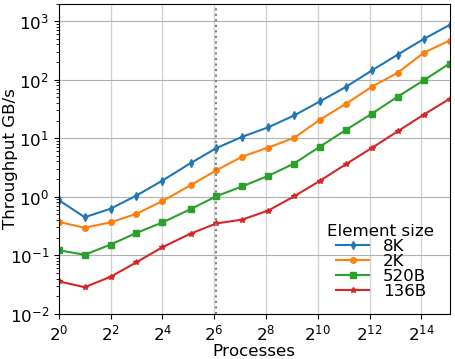
\includegraphics[scale=0.70]{projects/2.3.1-PMR/2.3.1.14-UPCxx-GASNet/all-cori-knl-out-inserts-wait.png}
  \caption{Weak scaling of distributed hash table insertion on the KNL partition of NERSC's Cori platform. The dotted line represents the processes in one node.}
  \label{fig:dht}
\end{figure}



\paragraph{Recent Progress}

The most notable work in the past year has been in three areas:

\textbf{1. Memory Kinds.}
UPC++ ``memory kinds'' provide a unified abstraction for communication between
combinations of device (e.g. GPU) and host memory, possibly remote.  By
unifying the expression of data transfer among the various memories in a
heterogeneous system with different memory kinds, these abstractions enable ECP
applications to utilize accelerators within UPC++'s PGAS model.  The
abstraction enables hardware offload (when available) of device data transfers,
eliminating the need for the application to stage transfers through
intermediate buffers in host memory.  Support for such offload on the OLCF's
Summit has been demonstrated in an October 2020 memory kinds prototype
distributed to our stakeholders.

\textbf{2. Training and Outreach.}
The past year has included an increased focus on outreach.  This includes
presenting four training events, and preparation of a fifth to appear at SC20.
A two-hour ``Birds of a Feather'' event in August 2020 introduced current and
potential UPC++ users to the authors of successful UPC++-based applications.
Circulation of working group drafts of proposed enhancements (see below) has
been valuable to both the UPC++ team and our stakeholders to agree upon design
in advance of implementation.

\textbf{3. Productivity and Performance.}
With the core API specification and implementation of UPC++ complete, we have
shifted focus toward addressing improvements to productivity and performance,
especially in response to feedback from our stakeholders.  The most significant
example of this is addition of support for non-trivial serialization of
user-defined types, providing concise syntax for the common cases and
straight-forward mechanisms for more complex ones.

\paragraph{Next Steps}

The planned work for the near-term future includes the following:

\textbf{1. Memory Kinds.}
We will continue development of the October 2020 memory kinds prototype.  The
implementation, currently targeting the hardware in Summit, will be extended to
include other accelerators scheduled to appear in the early Exascale systems.
As with Summit, transfers will be offloaded to available hardware capabilities
by leveraging the parallel efforts in GASNet-EX.

\textbf{2. Productivity and Performance.}
With the help of our stakeholders, we will continue to identify and address
portions of the UPC++ implementation where performance tuning is most needed
and/or beneficial.  Similarly, we will continue to work with stakeholders to
identify and implement features which improve productivity.

\textbf{3. Outreach.}
We will continue to hold training events for users of UPC++ and circulating
working group drafts of productivity features (above) to solicit feedback.

\newpage
\input{projects/2.3.1-PMR/2.3.1.16-SICM/2.3.1.16-SICM}
\newpage
\subsubsection{\stid{1.17} Open~MPI for Exascale (OMPI-X)}\label{subsubsect:openmpi}

%% {\itshape

%% 	\begin{enumerate}
%% 	\item Rename this file to your project WBS-projectname.tex, for example 2.3.3.01-XSDK4ECP.tex.
%% 	\item Complete this template for your project.  Limit your text to two pages, not counting citations.
%% 	\item Please avoid changing the content of main.tex.
%% 	\item Put any references in a .bib file with the same root name, for example 2.3.3.01-XSDK4ECP.bib.
%% 	\item Remember to include any image files you reference in your text.
%%     \item The files 2.3.3.01-XSDK4ECP.tex, 2.3.3.01-XSDK4ECP.bib and xSDK-diagram.jpeg are included as examples for your reference.  You can remove them from what you upload.
%% 	\end{enumerate}
%% }

\paragraph{Overview}
%% \textit{Provide an overview of your project.  You might find that the introductory text from your Fall 2017 Project Summary \url{https://confluence.exascaleproject.org/display/1ST/Fall+2017+ECP+ST+Project+Summaries} useful as a starting draft.}

The OMPI-X project ensures that the Message Passing Interface (MPI)
standard, and its specific implementation in Open~MPI meet the needs
of the ECP community in terms of performance, scalability, and
capabilities or features. MPI is the predominant interface for
inter-process communication in high-end computing.  Nearly all of the
ECP application (AD) projects (93\%~\cite{Bernholdt:2018:SMU-tr})
and the majority of software technology (ST) projects
(57\%~\cite{Bernholdt:2018:SMU-tr}) rely on it.
With the impending exascale era, the
pace of change and growing diversity of HPC architectures pose new
challenges that the MPI standard must address.  The OMPI-X project is
active in the MPI Forum standards organization, and works within it to
raise and resolve key issues facing ECP applications and libraries.

Open~MPI is an open source, community-based implementation of the MPI
standard that is used by a number of prominent
HPC vendors as the basis for their commercial MPI offerings.   The
OMPI-X team is comprised of active members of the Open~MPI community,
with an extensive history of contributions to this community.
The OMPI-X project focuses on prototyping
and demonstrating exascale-relevant proposals under consideration by
the MPI Forum, as well as improving the fundamental performance and
scalability of Open~MPI, particularly for exascale-relevant platforms
and job sizes.
MPI users will be able to take advantage of these
enhancements simply by linking against recent builds of the Open~MPI
library.

In addition to MPI and Open~MPI, the project also includes two other products,
which are less visible to the end user, but no less important.
PMIx (Process Management Interface for Exascale) provides facilities for
scalable application launch, process wire-up, resilience, and coordination between runtimes.
It originated as a spin-off from the Open~MPI community, but is now developing a
community of its own as adoption grows.  Starting in FY20,
Qthreads (formerly WBS 2.3.1.15) is also part of the OMPI-X project.  Qthreads is a
user-level lightweight asynchronous thread library particularly focused on improving support for
multithreading in the context of network communications.  Both PMIx and Qthreads help the
OMPI-X project address key issues of performance and capability for exascale applications.


\paragraph{Key  Challenges}
%% \textit{Describe what is hard to do, why it is challenging.}
A number of aspects of ``exascale'' levels
of computing pose serious challenges to the ``tried and true'' message
passing model presented by MPI and its implementations, including Open~MPI.
%
Keeping pace with changes in HPC architecture is a major challenge.
Examples include massive node-level concurrency, driving the
growth of ``MPI+X'' programming approaches,
and the complex memory architectures, which make the placement of data
within memory more important. In the near-term, with GPUs dominating the exascale
environment, how code running on the GPUs interacts with MPI and inter-process
communications must also be addressed.  This will require both changes to the standard
and changes and improvements within implementations.
%
Performance and scalability become both more important and more
challenging as node counts increase
and memory per MPI rank trends downward.
%
Finally, as we identify solutions to these challenges that must be
``implemented'' within the MPI \emph{standard} rather than particular MPI libraries,
we must work within the much larger and broader MPI
community that may not always be attuned to the needs of computing at the largest scales.

\paragraph{Solution Strategy}
%% \textit{Describe your basic strategy for addressing the challenges.}
The OMPI-X project is working across a number of fronts to address
these challenges.

\emph{Runtime Interoperability for MPI+X and Beyond} MPI is
increasingly being used concurrently with other runtime environments.
This includes both ``MPI+X'' approaches, where X
is most often a threading model, such as OpenMP, as
well as the use of multiple inter-process runtimes within a single
application.  Concerns include awareness of other runtimes,
cooperative resource management capabilities, and ensuring that all
concurrently active runtimes make progress.  We are developing APIs and
demonstrating capabilities for interoperability in both MPI+X and
multiple inter-process runtime situations.

\emph{Extending the MPI Standard to Better Support Exascale
Architectures} The MPI community is standardizing a
number of ideas that
are particularly important to supporting
the architectural and system size characteristics anticipated for
exascale.  ``Partitioned communications'' (previously called ``Finepoints'')
deal with the growing use of threading for node-level concurrency, in
combination with MPI.  ``Sessions'' increases the flexibility of MPI
semantics in a number of areas, which in turn can open opportunities
for enhanced scalability, as well as easier support for
multi-component applications such as coupled multi-physics
simulations. Error management and recovery capabilities are key to
ensuring that applications can detect and respond effectively when errors,
inevitably, occur during execution.  We are helping to drive incorporation
of these and other ideas into the MPI standard by developing prototypes and
working with ECP teams and the broader community to demonstrate their
feasibility and value.

\emph{Open~MPI Scalability and Performance} As we push the scale of
both hardware and applications, we stress MPI implementations and
expose areas that need to be improved.
OMPI-X is targeting key components within Open~MPI, such as threading capabilities,
memory usage, remote memory access (RMA), tag matching, and other areas,
for improvements in both scalability and performance.

\emph{Supporting More Dynamic Execution Environments} We are
developing and implementing strategies to help MPI applications
better deal with topological process layout preferences
and contention in the network.

\emph{Resilience in MPI and Open~MPI} Concerns about system and
application resilience increase as either scales in size.  Our goal in
this area is to ensure that MPI, Open~MPI, and PMIx provide not only
support for simplified
recovery for the widely used checkpoint/restart fault tolerance strategy, but also the building
blocks to support more general error management and recovery by applications (the evolution of the User-Level
Fault Mitigation concept). We work within the MPI Forum, implement,
and train users on resilience strategies.

\emph{MPI Tools Interfaces}  Several interfaces within the
MPI standard are primarily used to support performance and
correctness tools.
The MPI Forum is in the process
of making significant revisions and extensions to these interfaces.
We will track the discussions in the Forum and provide prototype
implementations within Open~MPI to facilitate evaluation and provide
feedback.
We will work with the
ECP community, including tool developers, to make additional data
available through the MPI\_T interface.

\emph{Quality Assurance for Open~MPI}  We are enhancing the
Open~MPI testing infrastructure, adding tests to reflect ECP
requirements, and instantiating routine testing on systems of
importance to ECP, both for correctness and performance.

\begin{figure}
\centering
\begin{minipage}[c]{0.20\textwidth}
\captionsetup{width=\textwidth,font=small,labelfont=bf} %% Need to override default width
\caption{Partitioned communications enables increased concurrency in communication operations which can be carried out by multiple threads or tasks.}
\label{fig:partitioned-communications}
\end{minipage}
\qquad
\begin{minipage}[c]{0.20\textwidth}
\includegraphics[width=\textwidth]{projects/2.3.1-PMR/2.3.1.17-OMPI-X/partitioned-communications-partial-sends.png}
\end{minipage}
\qquad
\begin{minipage}[c]{0.33\textwidth}
\includegraphics[width=\textwidth]{projects/2.3.1-PMR/2.3.1.17-OMPI-X/partitioned-communications-early-receive.png}
\end{minipage}
\end{figure}

\begin{wrapfigure}{r}{0.40\textwidth}
\includegraphics[width=0.40\textwidth]{projects/2.3.1-PMR/2.3.1.17-OMPI-X/reinit.png}
\caption{ReInit reduces application recovery time.}
\label{fig:reinit}
\end{wrapfigure}

\paragraph{Recent Progress}
%% \textit{Describe what you have done recently.  It would be good to
%% have some kind of figure or diagram in this section.}
Through extensive efforts with the MPI Forum community this year, OMPI-X has been successful in 
introducing a number of important exascale-related features into the forthcoming MPI 4.0 standard.
These include sessions, partitioned communications, and a number of error management and recovery features
based on the long-standing User-Level Fault Mitigation (ULFM) concept.  These capabilities have at least
prototype-level implementations available in the Open~MPI library, allowing interested project teams to start
exploring the new capabilities.  We also undertook a cleanup of the Open~MPI code base to improve the quality
of the implementation of some key error handling features. (As in many standards communities, distinctions 
sometimes need to be made between conformance with the standard and providing a ``high-quality'' implementations.)

We are also continuing to drive forward on a number of fronts that did not make the 4.0 version of the standard,
but are still considered important or useful for exascale and the ECP community, particularly in the context of resilience. The ULFM
proposal has been updated to reflect those features that have been incorporated into 4.0, as well as the discussions
within the Forum.  For the complementary Reinit simplified checkpoint/restart proposal (Figure~\ref{fig:reinit}), we have carried out a formal verification on the recovery algorithm. 
This ensures that the protocol, which we plan to propose for a future version of MPI, correctly handles the recovery phase 
of a failure response, including correct propagation of notifications, absence of deadlocks, and proper termination.

We have provided initial implementations of the features above, and more, within the context of the Open~MPI library, to allow
users to explore the new capabilities.  In addition to sessions and partitioned communications, we have expanded the
MPI\_T interface implementation to include events, and implemented a number of new events and performance variables,
demonstrating their use in the context of ECP miniapplications and tools.

Motivated largely by support for the Partitioned Communications proposal and other situations where high network 
concurrency is required, a general user-level threading abstraction has been developed to support both the Qthreads 
and BOLT/Argobots threading libraries within either the Open~MPI or MPICH libraries.  Work begun last year, in 
collaboration with the MPICH and Argobots ECP teams (WBS 2.3.1.07 and 2.3.5.05), has now been integrated into the two MPI implementations.
An important part of the work within Open~MPI involved abstracting the threading layer so that it was not limited to pthreads.

Work on integration with hardware and software environments specifically relevant to the exascale systems continues as well.  On the software
side, we have implemented support for the ALCF's Cobalt resource management system in Open~MPI and PMIx.  This work, which was necessitated by
a major refactoring of Open~MPPI to exclusively use PMIx as its low-level runtime layer, will facilitate support for Aurora, 
which will use a successor to Cobalt.  Combining both software and hardware, we have been working with the SICM ECP project
(WBS 2.3.1.16) to integrate support for complex memory hierarchies into Open~MPI based on SICM's APIs.  This work has now
been demonstrated in several contexts within the Open~MPI library, including the ability to selectively place objects in
either GPU HBM memory or DRAM.  We have also provided a design document for library developers
to work with different memory pools in the context of Open~MPI.  Finally, on the hardware side, we have benefit
working with HPE (Cray) to ensure that the new partitioned communication capability in MPI 4.0 will support GPUs effectively.

In addition to these activities, we continue to support quality assurance of the Open~MPI code base through more and better testing.  The Open~MPI testing infrastructure, 
MTT, continues to be improved for flexibility and capability.  One of this year's noteworthy efforts was the addition of the bueno application test harness to the testing 
system.  The facilitates incorporating third-party test cases (i.e. based on user applications) into the routine testing process without having to commit them to the
Open~MPI testing repository.

\paragraph{Next Steps}
%% \textit{Describe what you are working on next.}
In FY21 and beyond, we plan to continue working across the multiple fronts described above.  We will be in a much better position to work with application teams who can benefit from the new capabilities embodied in MPI 4.0, but who have been reluctant to adopt them until they were officially part of the standard.  We will likewise continue to identify and improve performance and scalability bottlenecks, and to work with HPE (Cray) and the larger community to ensure that their Slingshot network and GPU support are ready for Frontier and Aurora.

\newpage
%  The RAJA text is out-of-date.  Need to comment it out.
%
%\subsubsection{\stid{1.18} ISC4MCM (RAJA)} 
%
%\paragraph{Overview.} 
%The Integrated Software Components for Managing Computation and Memory 
%Interplay at Exascale (ISC4MCM) project is providing software libraries that 
%enable application and library developers to meet advanced architecture 
%portability challenges. The project goals are to enable writing performance 
%portable computational kernels and coordinate complex heterogeneous memory 
%resources among components in a large integrated application. These 
%libraries enhance developer productivity by insulating them from much of the 
%complexity associated with parallel programming model usage and 
%system-specific memory concerns.
%
%The software products provided by this project are three complementary and 
%interoperable libraries:
%\begin{enumerate}
%\item {\bf RAJA:} Software abstractions that enable C++ developers to write
%  performance portable (i.e., single-source) numerical kernels (loops). 
%\item {\bf CHAI:} C++ ``managed array'' abstractions that enable transparent
%  and automatic copying of application data to execution memory spaces at run
%    time as needed based on RAJA execution contexts.
%\item {\bf Umpire:} A portable memory resource management library that provides
%  a unified high-level API for resource discovery, memory provisioning,
%    allocation, access, operations, and introspection.
%\end{enumerate}
%
%Capabilities delivered by these software efforts are needed to manage the
%diversity and uncertainty associated with current and future HPC architecture
%design and software support. Moving forward, ECP applications and libraries 
%need to achieve performance portability: without becoming bound to particular
%(potentially-limiting) hardware or software technologies, by insulating 
%numerical algorithms from platform-specific data and execution concerns, and 
%without major disruption as new machine, programming models, and vendor
%software become available.
%
%These libraries in development in this project are currently used in production
%ASC applications at Lawrence Livermore National Laboratory (LLNL). They are
%also being used or being explored/adopted by several ECP application and
%library projects, including: LLNL ATDM application, GEOS (Subsurface), SW4
%(EQSIM), MFEM (CEED co-design), and SUNDIALS.
%
%The software projects are highly-leveraged with other efforts. Team members
%include: ASC and ATDM application developers, ASD tool developers, university
%collaborators, and vendors. This ECP ST project supports outreach to the ECP
%community and collaboration with ECP efforts.
%
%\paragraph{Key Challenges.}
%
%The main technical challenge for this project is enabling production
%applications to achieve performance portability in an environment of rapidly
%changing, disruptive HPC hardware architecture design. Typical large
%applications contain $O(10^5) - O(10^6)$ lines of code and $O(10K)$ loop
%kernels. The codes must run efficiently on platforms ranging from laptops to
%commodity clusters to large HPC platforms. The codes are long-lived and are
%used daily for decades, so they must be portable across machine generations.
%Also, the codes are under continual development, with a steady stream of new
%capabilities added throughout their lifetimes -- continual validation and
%verification is essential, which precludes substantial rewrites from scratch.
%Lastly, the complex interplay of multiple physics packages and dozens of
%libraries makes it so that the data required for the full set of components
%needed for a given simulation may not fit into a single system memory space. To
%advance scientific computing capabilities, applications must navigate these
%constraints while facing substantial hardware architecture disruption along the
%road toward Exascale computing platforms. 
%
%While the software provided by this project has a substantial user base at
%LLNL, achieving broader adoption in the ECP (projects without LLNL involvement,
%in particular) is another challenge. The software efforts are funded almost
%entirely by LLNL programs and the majority of their developers work on LLNL
%application projects. So resource limitations is a key issue.
%
%\paragraph{Solution Strategy.}
%
%The software libraries in this project focus on encapsulation and 
%application-facing APIs to insulate users from the complexity and 
%challenges associated with diverse forms of parallelism and heterogeneous 
%memory systems. This approach allows users to exploit new capabilities 
%with manageable rewriting of their applications.
%
%RAJA provides various C++ abstractions for parallel loop execution. It
%supports: various parallel programming model back-ends, such as OpenMP 
%(CPU multithreading and target offload), CUDA, Intel Threading Building Blocks,
%etc.; loop iteration space and data view constructs to reorder, 
%aggregate, tile, and partition loop iterations; complex loop kernel 
%transformations for optimization, such as reordering loop nests, fusing 
%loops, etc. RAJA also supports portable atomic operations, parallel scans, 
%and CPU and GPU shared memory. After loops have been converted to RAJA, 
%developers can explore implementation alternatives via RAJA features without 
%altering loop kernels at the application level.
%
%CHAI provides C++ ``managed array'' abstractions that automatically copy 
%data to execution memory spaces as needed at run time based on RAJA execution 
%contexts. Access to array data in loop kernels looks the same as when using
%traditional C-style arrays.
%
%Umpire provides a portable API for managing complex memory resources by 
%providing uniform access to other libraries and utilities that provide
%system-specific capabilities. Umpire decouples resource allocation from 
%specific memory spaces, allocators, and operations. The memory introspection 
%functionality of Umpire enables applications and libraries to make memory 
%usage decisions based on allocation properties (size, location, sharing 
%between packages, etc.)
%
%All three software libraries are open source and available on
%GitHub~\cite{RAJA-github, CHAI-github, Umpire-github}. There they provide
%regular software and documentation releases. Each project has dedicated email
%lists, issue tracking, test suites, and automated testing.
%
%\paragraph{Recent Progress}
%
%In FY18, CHAI and Umpire have been released as open source software projects
%and they are now developed on GitHub Recent development has focused on 
%user documentation and cleaner integration of these two libraries to give 
%applications more flexible and easy access to their capabilities.
%
%Many new features have been added to RAJA in FY18 to enable flexible
%loop transformations for complex loop kernels via execution policies.
%LLNL applications are assessing this new functionality now in a 
%"pre-release" version; it will be generally available before the end of FY18.
%
%The RAJA Performance Suite~\cite{RAJAPerf-github} was released and made 
%available on Github in January 2018. The Suite is used to assess and track 
%performance of RAJA across programming models and diverse loop 
%kernels. It is also being used for compiler acceptance testing in the CORAL 
%procurement and was prepared for use as a benchmark for the CORAL-2 procurement.
%
%In 2018, the RAJA project expanded its visibility beyond DOE NNSA Labs. 
%Recent presentations include a RAJA tutorial at the 2018 ECP Annual Meeting 
%and an application use case study the 2018 NVIDIA GPU Tech Conference (GTC). 
%Future tutorials are planned at 2018 ATPESC and GTC 2019. Also, a RAJA paper 
%and $1/2$-day tutorial proposal were submitted to SC18.
%
%\paragraph{Next Steps}
%
%Our next efforts include:
%\begin{enumerate}
%\item {\bf Fill RAJA Gaps:} Not all features are available for all programming
%  model back-ends; as models mature, such as OpenMP4.5, these gaps will be
%    filled.
%\item {\bf Expand RAJA User Guide and Tutorial:} Build example codes and user
%  documentation for latest RAJA features and prepare for future tutorials
%    (ATPESC 2018 and SC18).
%\item {\bf Expand RAJA Performance Suite:} Include kernels that exercise more
%  application use cases and RAJA features.
%\item {\bf Focus RAJA Vendor Interaction:} Work with CORAL vendors to address
%  issues as applications port to the Sierra platform at LLNL; establish early
%    interactions with CORAL-2 vendors to ensure RAJA will be supported well on
%    CORAL-2 systems.
%\item {\bf Expand Umpire Capabilities:} Explore potential collaboration with
%  relevant ECP efforts, such as SICM project.
%\end{enumerate}
\subsubsection{\stid{1.18} RAJA/Kokkos} 

\paragraph{Introduction}
The RAJA/Kokkos sub-project is a new combined effort intended to focus on collaborative development of backend capabilities for the Aurora and Frontier platforms.  The formation of this project is significant in that it bring two independent teams, RAJA (primarily from LLNL) and Kokkos (primarily from Sandia), to work on a common goal. This project also enhances interactions with staff from other labs, in particular Argonne and Oak Ridge, to help integrate RAJA and Kokkos into the software stack and applications at the respective leadership computing facilities.  The remainder of this section is focused on the Kokkos-specific activities since RAJA and integrated content were not available at the time of publication.


\paragraph{Overview} 

The Kokkos C++ Performance Portability Ecosystem is a production-level solution for writing modern C++ applications in an hardware-agnostic way.
Started by Sandia National Laboratories, it is now supported by developers at the Argonne, Berkeley, Oak Ridge, Los Alamos and Sandia National Laboratories as well as the Swiss National Supercomputing (Centre).
It is now used by more than a hundred HPC projects, and Kokkos-based codes are running regularly at-scale on half of the top ten supercomputers in the world. 
The EcoSystem consists of multiple libraries addressing the primary concerns for developing and maintaining applications in a portable way.
The three main components are the Kokkos Core Programming Model, the Kokkos Kernels Math Libraries and the Kokkos Tools.
Additionally, the Kokkos team is participating in the ISO C++ standard development process, to get successful concepts from the Kokkos EcoSystem incorporated into the standard. 
Its development is largely funded as part of the Exascale Computing Project, with a mix of NNSA ATDM and Office of Science sources. 

 
\paragraph{Key Challenges}

One of the biggest challenges for the ExaScale supercomputing era is the proliferation of different computer architectures, and their associated mechanisms to program them.
Vendors have an incentive to develop their own models in order to have maximum freedom of exposing special hardware capabilities, and potentially achieve "vendor-lock-in".
This poses the problem for applications that they may need to write different variants of their code for different machines - an effort which can be simply not feasible for many of the larger application and library projects.

The Kokkos project aims at solving this issue by providing a programming solution which provides a common interface build upon the vendor specific software stacks.
There are a number of technical challenges associated with that. 
First an abstraction must be designed which is restricted enough to allow mapping to a wide range of architectures while allowing exploitation of all the hardware capabilities provided by new architectures. 
Secondly, the development of support for a new architecture may take significant resources. In order to provide a timely solution for applications in line with the availability of the machine, CoDesign collaborations with the vendors are critical.
At the same time software robustness, quality and interface stability is of utmost importance. 
In contrast to libraries such as the BLAS, programming models permeate the entire code base of an application, and are not isolated to simple call sites. 
API changes thus would require a lot of work inside of the users code base. 
A fourth challenge is that in order to debug and optimize the code base tools are required to gain insights into the application. 

Besides the technical challenges, 
a comprehensive support and training infrastructure is absolutely critical for a new programming model to be successful.
Prospective users must learn how to use the programming model, current users must be able to bring up issues with the development team and access detailed documentation, and the development team of the model must be able to continue technical efforts without being completely saturated with support tasks. 
The latter point became a significant concern for the Kokkos team with the expected growth of the user base through ECP.  
Already before the launch of ECP, there were multiple application or library teams starting to use Kokkos for each developer on the core team -- a level not sustainable into the future without a more scalable support infrastructure. 
This issue was compounded by the fact that Kokkos development was funded through NNSA projects, making it hard to justify extensive support for open science applications. 

\paragraph{Solution Strategy}

To address the challenges the Kokkos team is developing a set of libraries and tools which allow application developers to implement, optimize and maintain performance portable codes. 
At its heart the EcoSystem provides the Kokkos Core Programming Model.
Kokkos Core is a programming model for parallel algorithms that use many-core chips and share memory among those cores.
The programming model includes abstractions for frequently used parallel execution patterns, policies that provide details for how those patterns are executed, and execution spaces that denote on which execution agents the parallel computation is performed. 
Kokkos Core also provides fundamental data structures with policies that provide details for how those data structures are laid out in memory, memory spaces that denote in which memory the data reside, and data access traits conveying special data access semantics.
The model works by requiring that application development teams implement their algorithms in terms of Kokkos’ patterns, policies, and spaces. 
Kokkos Core can then map these algorithms onto the target architecture according to architecture-specific rules necessary to achieve best performance.

Kokkos Kernels is a software library of linear algebra and graph algorithms used across many HPC applications to achieve best (not just good) performance on every architecture. The baseline version of this library is written using the Kokkos Core programming model for portability and good performance. The library has architecture-specific optimizations or uses vendor-specific versions of these mathematical algorithms where needed. This reduces the amount of architecture-specific software that an application team potentially needs to develop, thus further reducing their modification cost to achieve “best in class” performance. 

Kokkos Tools is an innovative “plug in” software interface and a growing set of performance measurement and debugging tools that plug into that interface for application development teams to analyze the execution and memory performance of their software. Teams use this performance profiling and debugging information to determine how well they have designed and implemented their algorithms and to identify portions of their software that should be improved. Kokkos Tools interfaces  leverage the Kokkos Core programming model interface to improve an application developer’s experience dramatically, by forwarding application specific information and their context within the Kokkos Core programming model to the tools.

Kokkos Support addresses the challenges of establishing, growing and maintaining the user community.
First and foremost, it provides explicit means for supporting all DOE ECP applications. 
A main component of that is funding for local Kokkos experts at the Sandia, Oak Ridge, Argonne, Berkeley and Los Alamos laboratories which can serve as direct contacts for local applications and the users of the leadership computing facilities. 
Secondly, the project develops and maintains a reusable support infrastructure, which makes supporting more users scalable and cost effective. 

The support infrastructure consists of GitHub wiki pages for the programming guide and API reference, GitHub issues to track feature requests and bug reports, a Slack channel for direct user-to-user and user-to-developer communication, and tutorial presentations and cloud-based Kokkos hands-on exercises. 

The Kokkos Team is also actively engaging the ISO C++ Committee, where it provides about a third of the members interested in HPC.
This strong engagement enables the team to lead or contribute to numerous proposals.
Among those proposals the team leads are abstractions for multi dimensional arrays based on Kokkos View, atomic operations on generic types and linear algebra algorithms based on Kokkos Kernels, which cover not only the classic Fortran BLAS capabilities, but also batched BLAS and mixed precision linear algebra.
The team also has a central role in the primary proposal introducing heterogeneous computing into the C++ standard via the executors concept.

\paragraph{Recent Progress}

The Kokkos project now consists of an integrated developers team spanning five DOE National Laboratories.
In particular both NNSA and Office of Science funded developers are working based off the same task and code management system, use a shared slack channel, and attend a common weekly team meeting.
This ensures that no duplication of effort happens, and makes Kokkos a true inter laboratory project.

Kokkos is now used by many applications in production across the entire spectrum of DOE's super computers.
Support for current production platforms is mature and stable.
Work on supporting the upcoming ExaScale platforms has begun and initial capabilities for AMD GPUs and Intels GPUs are working.
On the AMD side this is despite the fact that full support was previously available, but had to be removed due to the deprecation of the underlying programming model by AMD.

Three Kokkos specific multi-day boot camps were organized with a total attendance on the order of 60 developers.
Additionally the team provided single day tutorials at numerous venues with several hundred attendees in aggregate.
The slack channel now sees daily questions from numerous users, and has attracted even vendor representatives who help answer machine specific questions.
The team finished developing a full API documentation as well as adding use case descriptions for common patterns found in applications.

At the C++ committee, the MDSpan proposal is now in wording review - meaning that the technical design is approved. 
MDSpan will be able to provide all the core capabilities of Kokkos\:\:View.
This includes compile and runtime extents, customizable layouts, and data access traits.
The extension to heterogeneous memory can be achieved by trivial extensions. 
Furthermore, the atomic\_ref proposal was voted into C++20.
This capability will provide atomic operations on generic allocations as powerful as Kokkos' atomic operations.
In particular it allows atomic operations on types independent of their size, and not just the ones native in the hardware.
A very recent development, is the proposal for linear algebra functions.
It entails functionality covering all of BLAS 1, 2, and 3, but extends it to any scalar types (including mixing of scalar types) and batched operations.
The proposal was approved by the relevant study groups, as well as the library evolution incubator group.
The Kokkos team was also able to gain co-authors from NVIDIA, Intel and AMD - providing significant support from the leading hardware vendors.

\paragraph{Next Steps}

The most pressing next task is to complete and then mature support for the upcoming ExaScale architectures.
Most of Kokkos's functionality is expected to be available by the end of FY20 for those systems, which will provide another year of time to mature the support before the first platforms will be delivered.

On the programming model evolution side, more explicit asynchronous capabilities including the creation of graphs of kernel launches is a high priority.

At the plumbing level, the team will start to replace some of the implementation level of Kokkos by the ISO C++ capabilities such as atomic\_ref and mdspan.

For Kokkos tools an upcoming capability will be the addition of autotuning tools. This will help with the increasingly difficult task of coming up with heuristics to determine good runtime settings for kernels on all the different architectures.

And last but not least, the team will work on getting the proposed new ISO C++ capabilities into the C++23 draft standard, so that they will be available to our users as a vendor provided capability during the lifetime of the first ExaScale platforms.

\newpage
\input{projects/2.3.1-PMR/2.3.1.19-Argo-PowerSteering/2.3.1.19-Argo-PowerSteering}
\newpage

%\subsection{\tools}
%This section presents projects in \tools.
\subsection{\stid{2} \tools}\label{subsect:tools}

\textbf{End State:}	A suite of development tools and supporting unified infrastructure aimed at improving developer productivity across increasingly complex architectures, especially those targeted for Exascale platforms.


\subsubsection{Scope and Requirements}
For Exascale systems, the compilers, profilers, debuggers, and other software development tools must be increasingly sophisticated to give software developers insight into the behavior of not only the application and the underlying hardware but also the details corresponding to the underlying programming model implementation and supporting runtimes (e.g., capturing details of locality and affinity). These capabilities should be enhanced with further integration into the supporting compiler infrastructure and lower layers of the system software stack (e.g., threading, runtime systems, and data transport libraries), and hardware support. Most of the infrastructure will be released as open source, as many of them already are, with a supplementary goal of transferring the technology into commercial products. Given the diversity of Exascale systems architectures, some subset of the tools may be specific to one or more architectural features and is potentially best implemented and supported by the vendor; however, the vendor will be encouraged to use open APIs to provide portability, additional innovation, and integration into the tool suite and the overall software stack.


\subsubsection{Assumptions and Feasibility }

The overarching goal of improving developer productivity for Exascale platforms introduces new issues of scale that will require more lightweight methods, hierarchical approaches, and improved techniques to guide the developer in understanding the characteristics of their applications and to discover sources of the errors and performance issues. Additional efforts for both static and dynamic analysis tools to help identify lurking bugs in a program, such as race conditions, are also likely needed. The suite of needed capabilities spans interfaces to hardware-centric resources (e.g., hardware counters, interconnects, and memory hierarchies) to a scalable infrastructure that can collect, organize, and distill data to help identify performance bottlenecks and transform them into an actionable set of steps and information for the software developer. Therefore, these tools share significant challenges due to the increase in data and the resulting issues with management, storage, selection, analysis, and interactive data exploration. This increased data volume stems from multiple sources, including increased concurrency, processor counts, additional hardware sensors and counters on the systems, and increasing complexity in application codes and workflows.

Compilers obviously play a fundamental role in the overall programming environment but can also serve as a powerful entry point for the overall tool infrastructure. In addition to optimizations and performance profiling, compiler-based tools can help with aspects of correctness, establishing connections between programming model implementations and the underlying runtime infrastructures, and auto-tuning. In many cases, today's compiler infrastructure is proprietary and closed source, limiting the amount of flexibility for integration and exploration into the Exascale development environment. In addition to vendor compiler options, this project aims to provide an open source compiler capability that can play a role in better supporting and addressing the challenges of programming at Exascale. 


\subsubsection{Objectives}

This project will design, develop, and deploy an Exascale suite of development tools built on a unified infrastructure for development, analysis, and optimization of applications, libraries, and infrastructure from the programming environments of the project. The overarching goal is to leverage and integrate the data measurement, acquisition, storage, and analysis and visualization techniques being developed in other projects of the software stack. The project will seek to leverage techniques for common and identified problem patterns and create new techniques for data exploration related to profiling and debugging and support advanced techniques such as autotuning and compiler integration. We will seek to establish an open-source compiler activity leveraging activities around the LLVM infrastructure. These efforts will require collaboration and integration with system monitoring and various layers within the software stack.


\subsubsection{Plan}
It is expected that multiple projects will be supported under the tools effort. To ensure relevance to DOE missions, most of these efforts shall be DOE laboratory led and leverage and collaborate with existing activities within the broader HPC community. Initial efforts will focus on identifying the core capabilities needed by the selected ECP applications, components of the software stack, expected hardware features, and the selected industry activities from within the Hardware and Integration focus area. The supported projects will target and implement early versions of their software on both CORAL and APEX systems, with an ultimate target of production-ready deployment on the Exascale systems. Throughout this effort the applications teams and other elements of the software stack will evaluate and provide feedback on their functionality, performance, and robustness. These goals will be evaluated yearly (or more often as needed) based on milestones as well as joint milestone activities shared across the associated software stack activities by AD and HI focus areas.

\subsubsection{Risks and Mitigations Strategies}

A risk exists in terms of adoption of the various tools and their supporting infrastructure by the broader community, including support by system vendors. Past experience has shown that a combination of laboratory-supported open source software and vendor-optimized solutions built around standard APIs that encourage innovation across multiple platforms is a viable approach, and this will be undertaken. We will track this risk primarily via the risk register.

Given its wide use within a range of different communities, and its modular design principles, the project's open source compiler activities will focus on the use of the LLVM compiler infrastructure as a path to reduce both scope and complexity risks and leverage with an already established path for NRE investments across multiple vendors. The compilers and their effectiveness are tracked in the risk register. 

Another major risk for projects in this area is the lack of low-level access to hardware and software necessary for using emerging architectural features. Many of these nascent architectural features have immature implementations and software interfaces that must be refined prior to release to the broader community. This project should be at the forefront of this interaction with early delivery systems. This risk is also tracked in the risk register for compilers, which are particularly vulnerable.

\subsubsection{Future Trends}

Future architectures are becoming more heterogeneous and complex~\cite{vetter:2018:extreme}. As such, the role of languages, compilers, runtime systems, and performance and debugging tools will becoming increasingly important for productivity and performance portability. 
%
In particular, our ECP strategy focuses on improving the open source LLVM compiler and runtime ecosystem; LLVM has gained considerable traction in the vendor software community, and it is the core of many existing heterogeneous compiler systems from NVIDIA, AMD, Intel, ARM, IBM, and others.  We foresee that this trend will continue, which is why we have organized the \tools\ technical area around LLVM-oriented projects.  
%
Many of our contributions to LLVM address these trends and will persist after ECP ends. 
%
For example, our contributions for directive-based features for heterogeneous computing (e.g., OpenMP, OpenACC) will not only provide direct capabilities to ECP applications, but it will also impact the redesign and optimization of the LLVM infrastructure to support heterogeneous computing.
%
In a second example, Flang (open source Fortran compiler for LLVM; [the second version is also known as F18]) will become increasingly important to the worldwide Fortran application base, as vendors find it easier to maintain and deploy to their own Fortran frontend (based on Flang).  
%
Furthermore, as Flang become increasingly robust, researchers and vendors developing new architectures will have immediate access to Flang, making initial Fortran support straightforward in ways similar to what we are seeing in Clang as the community C/C++ frontend.

%

\newpage
\subsubsection{\stid{2.01} \tools\ Software Development Kits} 

\paragraph{Overview}
The Software Development Tools SDK is a collection of independent projects specifically targeted to address performance analysis at scale. The primary responsibility of the SDK is to coordinate the disparate development, testing, and deployment activities of many individual projects to produce a unified set of tools ready for use on the upcoming exascale machines. The efforts in support of the SDK are designed to fit within the overarching goal to leverage and integrate data measurement, acquisition, storage, analysis, and visualization techniques being developed across the ECP Software Technology ecosystem.


\paragraph{Key Challenges}
In addition to the general challenges faced by all of the SDKs outlined in Section~\ref{subsubsect:ecosystem-sdk}, the unique position of the \tools\ SDK between the hardware teams and the application developers requires additional effort in preparing today’s software to run on yet-unknown architectures and runtimes to be delivered by the end of ECP.

\paragraph{Solution Strategy}
The primary mechanism for mitigating risk in the SDK is the \textit{Readiness Survey}. This survey is designed to assess the current status of each product in the SDK in six key areas: software availability, documentation, testing, Spack build support, SDK integration, and path forward technology utilization. By periodically assessing the progress of the individual L4 products in the SDK, we will use the survey to identify and resolve current hardware architecture dependencies, plan for future architecture changes, and increase adoption of the Continuous Integration (CI) testing workflow to reduce this risk.

Critically, the survey will allow us to accomplish this by providing a direct communication channel between the SDK maintainers and the L4 product developers allowing us to identify current architecture dependencies in each project and compare them with existing and emerging ECP platforms. Our initial efforts will be to increase support for today’s heterogeneous CPU architectures across the DOE facilities (e.g., x86, Power, ARM, etc.) to ensure a minimum level of usability on these platforms. We will then focus on current accelerator architectures- namely GPGPU computing. As new architectures arise, we will re-issue the survey and use this same process to provide guidance to the L4 product as they develop support for them.

The survey also allows us to monitor the increased adoption of the proposed ECP CI testing workflow. This will be crucial to understanding each project’s interoperability with not only the other projects within the Tools SDK, but all applications across the ECP Software Technologies landscape. Additionally, it will serve as a bridge between the Hardware Integration teams working with the facilities and the software teams working across the SDK. By relaying new hardware requirements from the facilities to the software developers, we can closely monitor support for both new and existing systems. Conversely, giving feedback to the facilities regarding compiler support and buildability of library dependencies will guide software adoption on those platforms.

\paragraph{Recent Progress}
The Readiness Survey was re-issued to each L4 product in July 2020. All projects had nominal changes except that HPCToolkit and TAU have added support for both Intel and AMD GPUs. With these changes,  four of the six L4 projects support NVIDIA GPUs, 3/6 support AMD, 2/6 support Intel, and 2/6 have support for all three GPU platforms.

The first step in assessing buildability of the L4 products was carried out in Q2 of FY20. All six projects were built on three platforms (Power9, x86, and Aarch64) using gcc and clang. Initially, only four successfully built with gcc on all platforms, and only one built with clang on any platform. The issues were reported and fixed, and now all six products build with gcc successfully on all three pre-exascale test platforms. The clang builds encountered a large number of issues in both the SDK products and their dependencies. The effort required to fix these issues was larger than the time allocated for the task, so they have been moved to Q1 FY21 as part of a larger procedure to assess LLVM/clang compatibility.

Support for automated testing remains a challenge area that all of the projects are aware of and plan to dedicate time to in FY21 and beyond. In Q2 of FY20, initial assessment of testing capabilties was carried out for two of the six products, Dyninst and TAU, on pre-exascale systems. With this work, both products now have working test suites that can be employed through scriptable executions. This represents an essential component of software sustainability to demonstrate and track correctness in the presence of code changes for these products.

Continuous Integration (CI) testing remains a still-larger challenge for the SDK. This is due in part to some products not having scriptable testing capabilities and also in part to more general challenges of using CI at the facilities through OSTI. With substantial help from Don Magrack at NMC and the CI team at ALCF, the first CI run was successfully carried out using Dyninst using Theta at the Argonne Leadership Compute Facilities in Q4 2020. We note that automated CI testing through OSTI remains as future work until the federated runners are established at the national labs.


\paragraph{Next Steps}
Additional testing using multiple compilers- including some variant of LLVM currently in use by the Compilers and Debuggers SDK- on at least one current DOE facility machine, and preferably one early access system, is our top priority for FY21. Results from these tests will continue to be fed back into the L4 products to further guide development of spack packages, bug/issue-reporting workflows, and integration into the greater ECP software ecosystem. Any discovered issues with Spack, compilers, or libraries will be directly reported back to their respective development teams or L3 representative.

Our KPP3 goals are tightly associated with integrating each L4 product into E4S, and a large part of these goals is getting more products using CI testing. As such, increasing the number of L4 products in the SDK with CI testing adoption is our second goal for FY21. The first CI workflow integration carried out in Q4 2020 established the basic procedure for getting the other products set up. Arguably, establishing this workflow is the largest contribution the Tools SDK will bring to the overall ECP software ecosystem. Having automated testing in place across heterogeneous build environments and target architectures is a fundamental challenge to creating reliable, sustainable software- making this work a critical path to attaining the ECP goals of large-scale software sustainability. We also anticipate that this may be the introduction of formal software testing for some of the L4 products. The heterogeneous nature of the testing available in the Tools SDK L4 products will serve as a focused testbed for constructing implementation guidelines for the CI workflow which can then be applied across the SDK efforts and into the greater ECP software ecosystem. Importantly, these lessons can also be carried on by the individual project teams to help maintain their software beyond the ECP timeline.

\newpage
\input{projects/2.3.2-Tools/2.3.2.06-EXA-PAPI/2.3.2.06-EXA-PAPI}
\newpage

\subsubsection{\stid{2.08} HPCToolkit} 
\paragraph{Overview} 

The HPCToolkit project is working to develop performance measurement
and analysis tools to help ECP application, library, runtime, and tool
developers understand where and why their software does not fully
exploit hardware resources within and across nodes of extreme-scale
parallel systems. Key deliverables of the project are a suite of
software tools that developers need to measure and analyze the
performance of parallel software as it executes on existing ECP
testbeds and new technologies needed to measure and analyze
performance on forthcoming GPU-accelerated exascale systems.

To provide a foundation for performance measurement and analysis, the
project team is working with community stakeholders, including
standards committees, vendors, and open source developers to improve
hardware and software support for measurement and attribution of
application performance on extreme-scale parallel systems. The
project team has been engaging vendors to improve hardware support
for performance measurement in next-generation GPUs and working
with other software teams to design and integrate new capabilities
into operating systems, runtime systems, communication libraries, and
application frameworks that will enhance the ability of software
tools to accurately measure and attribute code performance on
extreme-scale parallel systems.  Using emerging hardware and software
interfaces for monitoring code performance on both CPUs and GPUs, the project team is
working to extend capabilities to measure and analyze computation, data movement,
communication, and I/O as a program executes to pinpoint scalability
bottlenecks, quantify resource consumption, and assess
inefficiencies.

\paragraph{Key  Challenges}

Today's fastest supercomputers and forthcoming exascale systems all
employ GPU-accelerated compute nodes. Almost all of the 
computational power of GPU-accelerated compute nodes comes from GPUs rather than CPUs.
GPU-accelerated compute nodes have complex memory hierarchies that include 
multiple memory technologies with different bandwidth and latency characteristics. In addition, 
GPU-accelerated compute nodes have non-uniform connections between memories and computational elements (CPUs and GPUs). 
Furthermore, the next three DOE supercomputers (Perlmutter, Aurora, and Frontier) will feature GPUs from different vendors (NVIDIA, Intel, and AMD). 
There are significant differences in the underlying organization of these GPUs as well as their hardware and software support for performance measurement. For
performance tools, the need to support multiple CPU and GPU architectures significantly increases tool complexity.  At the same time, the
complexity of applications is increasing dramatically as developers
struggle to expose billion-way parallelism, map computation onto
heterogeneous computing elements, and cope with the growing complexity
of memory hierarchies. While application developers can employ
abstractions to hide some of the complexity of emerging parallel
systems, performance tools must be intimately familiar with each of
the features added to these systems to improve performance or
efficiency, develop measurement and analysis techniques that assess
how well these features are being exploited, and then relate these
measurements back to software to create actionable feedback that will
guide developers to improve the performance, efficiency, and
scalability of their applications.

\paragraph{Solution Strategy}

Development of HPCToolkit as part of ECP is focused on preparing it
for production use at exascale by enhancing it in several ways. First,
the team is adding new capabilities to measure and analyze
interactions between software and key hardware subsystems in
extreme-scale platforms, including GPUs and the complex memory hierarchies on GPU-accelerated compute nodes. A major focus of this effort is developing new capabilities for 
measurement and analysis of performance on GPUs.
Second, the team is working to improve performance
attribution given optimized code for a large collection of complex node-level programming
models used by ECP developers, including 
vendor specific programming models such as CUDA, HIP, and Data Parallel C++,
open source community programming models such as OpenMP,
and template-based programming models developed at national laboratories such as LLNL's RAJA and Sandia's KOKKOS. To support
this effort, the project team is enhancing the Dyninst binary analysis
toolkit, which is also used by other ECP tools. A major focus of this effort 
is to support analysis of GPU binaries. Third, the team is
improving the scalability of HPCToolkit so that it can be used to
measure and analyze extreme-scale executions. Fourth, the project team
is working to improve the robustness of the tools across the range of
architectures used as ECP platforms. Finally, the project team will
work other ECP teams to ensure that they benefit from HPCToolkit's
capabilities to measure, analyze, attribute, and diagnose performance
issues on ECP testbeds and forthcoming exascale systems.

\newpage
\paragraph{Recent Progress}

\begin{itemize}

\item
The project team developed a unified GPU monitoring substrate that supports GPUs from different vendors.
Based on the GPU-independent substrate, the project team developed kernel level measurement, 
which refers to the capability of collecting summary metrics for kernel launches, memory copies, and synchronizations,
for NVIDIA, Intel and AMD GPUs.

\item
The project team refined fine-grained measurement, which refers to the capability of collecting metrics inside a kernel, such as metrics for a device function, a basic block, a source line, or even a machine instruction, Nvidia GPUs.
Figure~\ref{fig:hpctoolkit}(a) shows a calling context that spans both CPU and GPU for a benchmark code implemented using LLNL's RAJA template-based programming model.
The team is also investigating fine-grained measurement for Intel GPUs and discussing fine-grained measurement support for AMD GPUs with AMD.

\item
The project team enhanced HPCToolkit for collecting and visualizing traces of both CPU and GPU activity.
Figure~\ref{fig:hpctoolkit}(b) shows a trace of a 6-process GPU-accelerated execution of a recent snapshot of Nyx---an adaptive mesh, compressible cosmological hydrodynamics simulation code being developed as part of the DOE ECP ExaSky project. In the figure, CPU trace lines appear as continuous multi-colored bands running the  trace lines the width of the figure. GPU trace lines show large intervals of white, indicating idleness, or red, indicating costly, excess synchronization present in the prototype code measured.

\item
The project team developed a novel approach that utilizes both shared and distributed memory parallelism to analyze and aggregate sparse data representations of performance measurements from every rank, thread and GPU stream in a program execution. 

\item 
The project team improved the reliability of HPCToolkit's hpcrun for monitoring complex dynamic library loading and unloading and interacting with the application when other software tools are present.

\end{itemize}

\begin{figure}[t]
\captionsetup{width=.96\textwidth}
\begin{minipage}[t]{.48\textwidth}
\centering
\includegraphics[width=\textwidth]{projects/2.3.2-Tools/2.3.2.08-HPCToolkit/hpctoolkit-raja-perf}
\\(a)
\end{minipage}
\hfill
\begin{minipage}[t]{.48\textwidth}
\centering
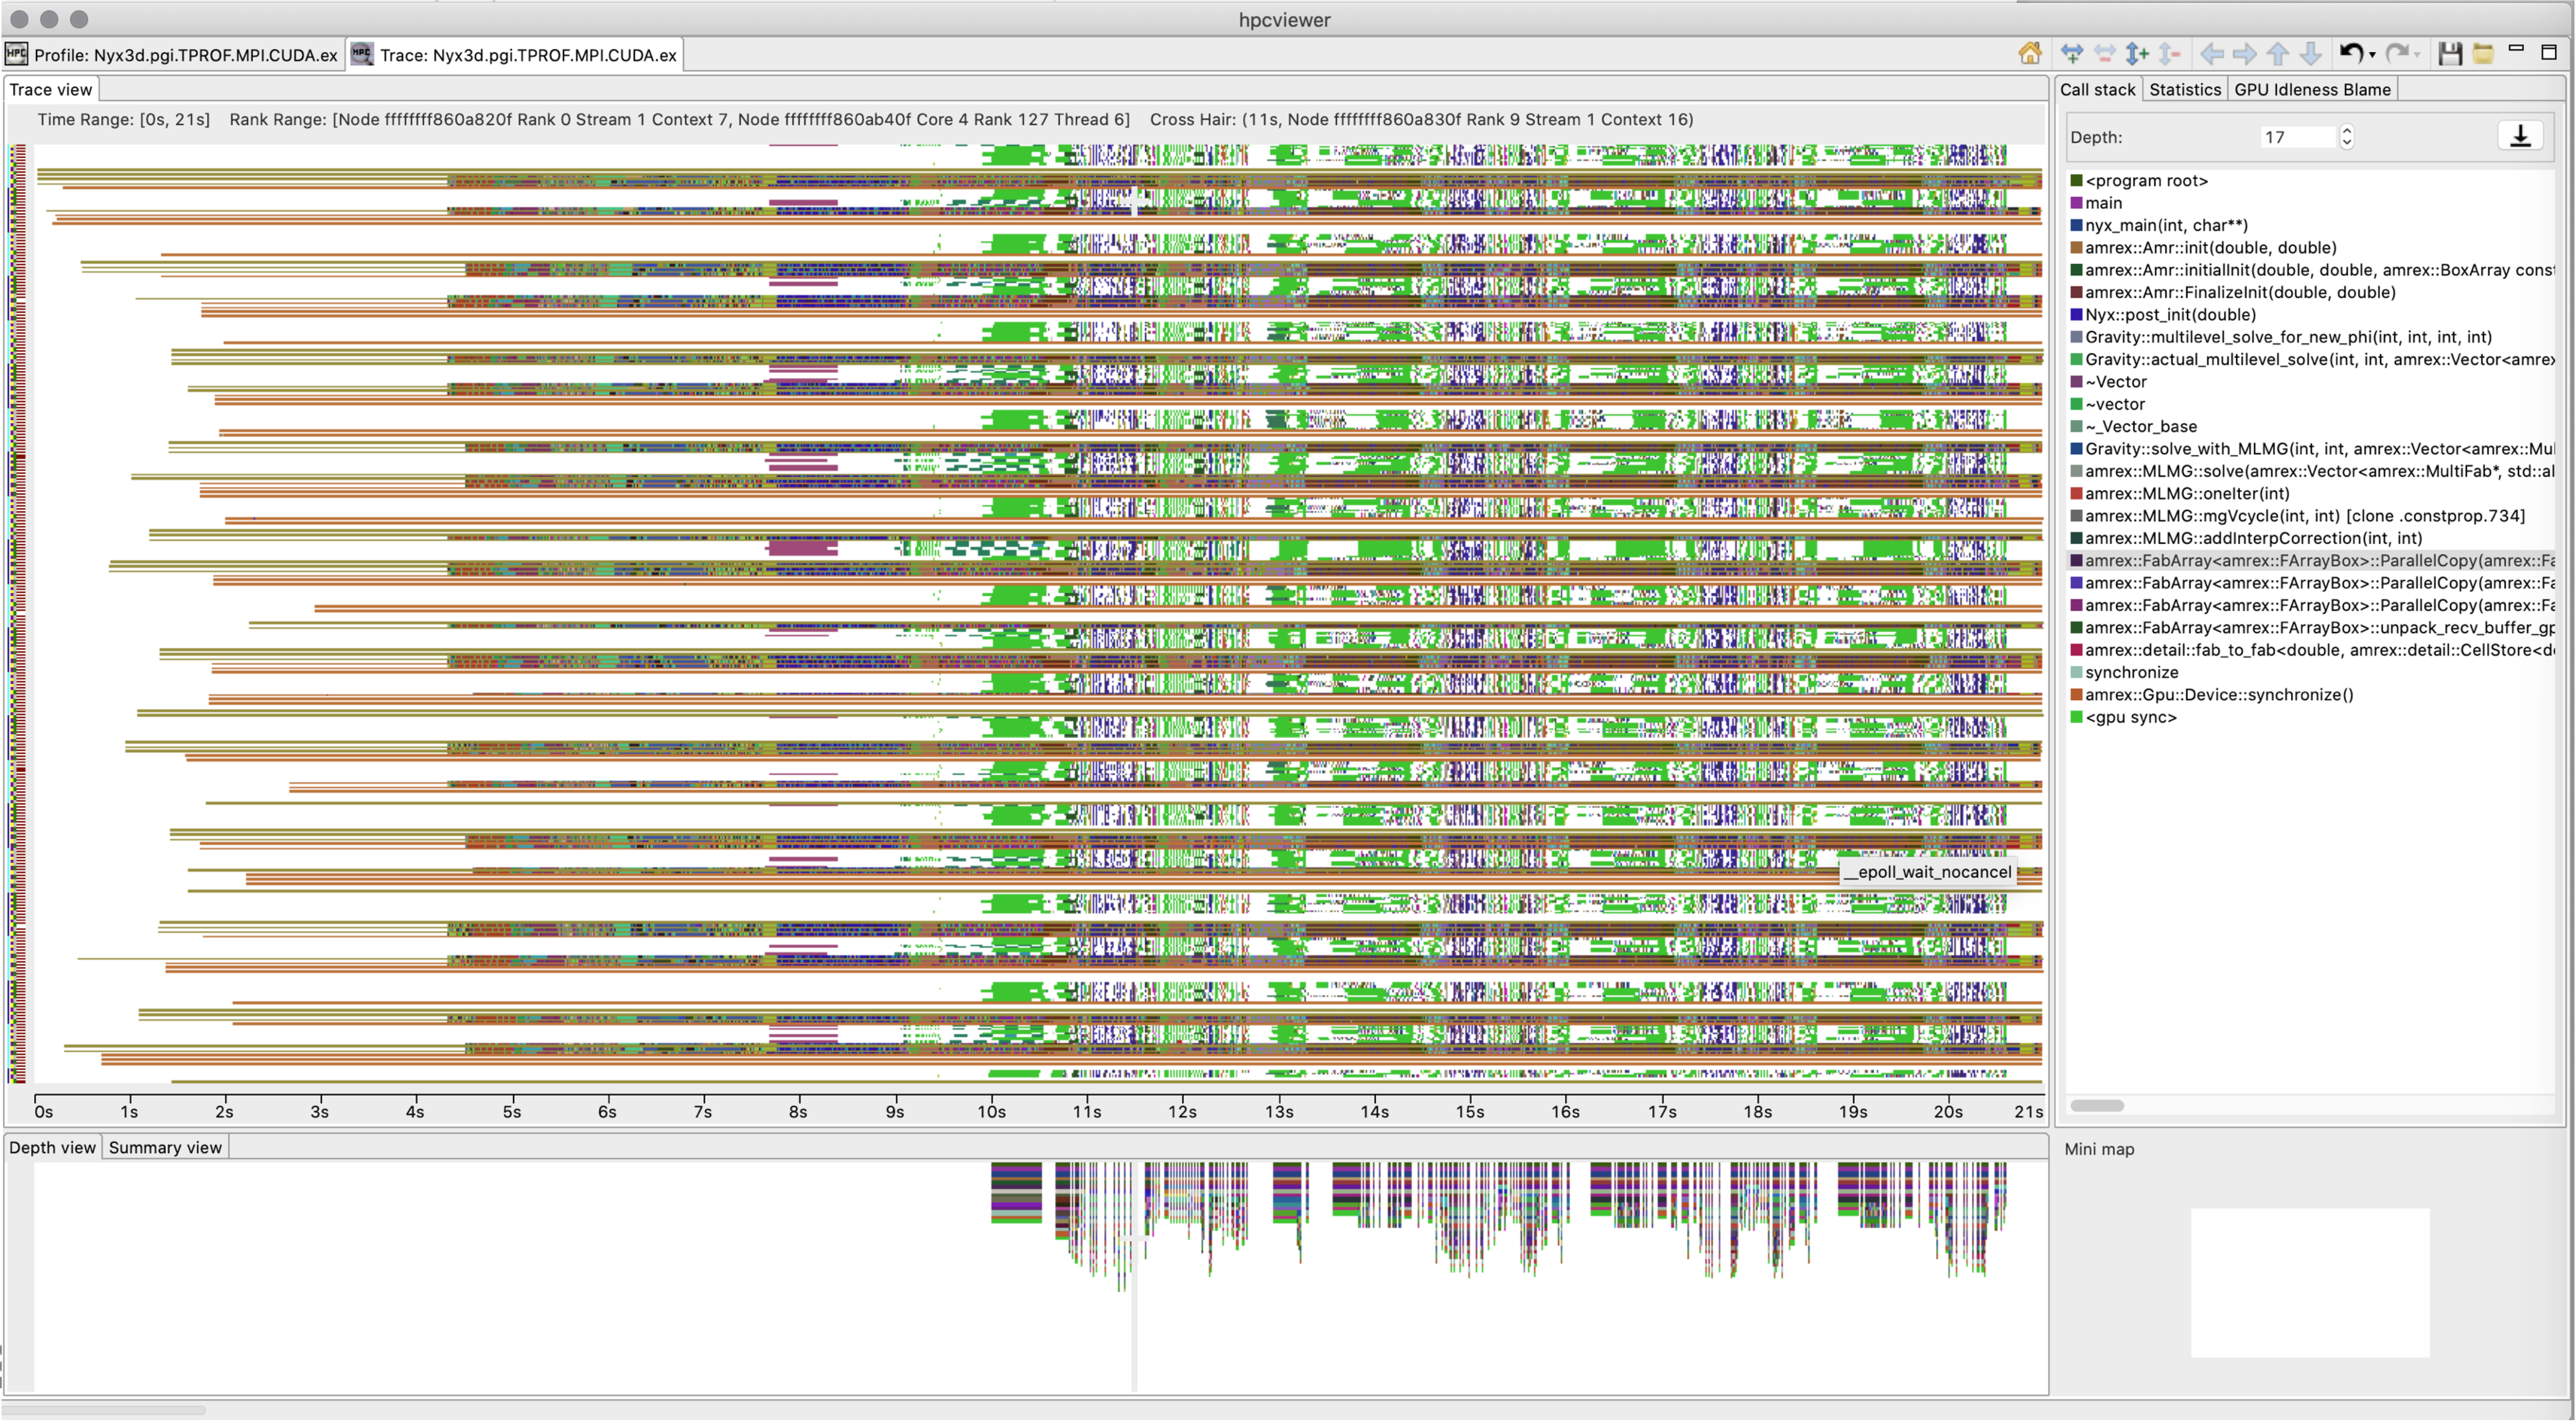
\includegraphics[width=\textwidth]{projects/2.3.2-Tools/2.3.2.08-HPCToolkit/hpctoolkit-nyx-trace}
\\(b)
\end{minipage}
\caption{(a) 
HPCToolkit's {\tt hpcviewer} showing a detailed attribution of GPU performance metrics in a 
profile of an optimized, GPU-accelerated benchmark written using LLNL's RAJA template-based programming model.
(b) HPCToolkit's {\tt hpctraceviewer} showing a 6-process GPU-accelerated execution trace of Nyx---an adaptive mesh, compressible cosmological hydrodynamics simulation code.}
\label{fig:hpctoolkit}
\end{figure}

\paragraph{Next Steps}
\begin{itemize}

\item 
Integrate GPU measurement and analysis capabilities into HPCToolkit's trunk for
release.

\item 
Continue to investigate solutions for fine-grained GPU performance measurement for Intel and AMD GPUs.

\item 
Continue to improve reliability of hpcrun for monitoring dynamic library loading and unloading

\item 
Work with the open source community to upstream GPU measurement support
developed by the project team into the community version of the {\tt
libomptarget} offloading library.

\item 
Work with DOE and platform vendors to evaluate and refine software interfaces for measuring GPU performance.

\end{itemize}

\newpage
\subsubsection{\stid{2.10} PROTEAS-TUNE: Programming Toolchain for Emerging Architectures and Systems} 

\paragraph{Key  Challenges:}
Programmer productivity and performance portability are two of the most important challenges facing users of future exascale computing platforms. Application developers targeting ECP architectures will find it increasingly difficult to meet these two challenges without integrated capabilities that allow for flexibility, composability, and interoperability across a mixture of programming, runtime, and architectural components. 

\paragraph{Solution Strategy:}
The PROTEAS-TUNE project was formed as a strategic response to this challenge. (The PROTEAS-TUNE project is the result of merger in FY20 of two previous ECP projects: PROTEAS [PROgramming Toolchain for Emerging Architectures and Systems] and Y-Tune: Autotuning for Cross-Architecture Optimization and Code Generation.) 
This project has three high-level goals. First, PROTEAS-TUNE will provide a programming pathway to anticipated exascale architectures by addressing programmability and portability concerns of emerging technology trends seen in emerging architectures. In particular, the project focuses on improvements to LLVM and OpenACC. Additionally, the team has significant experience with CUDA, OpenCL, and other programming models that will enable ECP applications teams to explore programming options to find the most effective and productive approaches without constraining programming models or software solutions. Second, PROTEAS-TUNE will prototype an integrated programming framework strategy will deliver solutions on these emerging architectures that will be further refined for these architectural capabilities, and make sure that they transition to vendors, standards activities, applications, and facilities. Thirdly, PROTEAS-TUNE includes autotuning which makes it possible to separate a high-level C/C++/FORTRAN implementation from architecture-specific implementation (OpenMP, OpenACC, CUDA, etc.), optimization, and tuning. It also provides a flexible programming framework and integrated toolchain that will provide ECP applications the opportunity to work with programming abstractions and to evaluate solutions that address the exascale programming challenges they face. 


Specifically, the PROTEAS-TUNE focuses on seven thrusts to improve capabilities and performance portability for applications on exascale architectures: 

\begin{itemize}
\item 
    Improve the core-LLVM compiler ecosystem; 
\item 
	Design and implement the OpenACC heterogeneous programming model for C/C++ in Clang/LLVM (Clacc);
\item 
    Design and implement the OpenACC heterogeneous programming model for Fortran in Flang/LLVM (Flacc);  
    
\item 
	Use performance modeling and optimization to enable code transformation and performance portability;
\item 
	Refine autotuning for OpenMP and OpenACC programming models in order to directly target challenges with heterogeneous architectures;
\item 
    Improve performance measurement and analysis tools (TAU) for the target exascale architectures and apply it to applications to improve performance;
\item 
    Develop and implement portable software abstractions (Papyrus) for managing persistent memory;
\item 
    Aggressively engage applications, SDK, vendor, and software teams to demonstrate and deploy; and,
\item
    in collaboration with SOLLVE and Flang, develop a DOE ECP fork of LLVM that will be the clearinghouse for ECP modifications of LLVM  (see \url{https://github.com/llvm-doe-org}).
    
\end{itemize}

Importantly, the team’s solutions are based on significant, continuing work with LLVM, OpenACC, OpenMP, ARES HLIR, OpenARC, TAU, SuRF and CHiLL. The team has extensive experience and a demonstrated track record of accomplishment in all aspects of this proposed work including existing software deployments, interaction with application teams, vendor interaction, and participation in open source community and standards organizations. Also, the team champions its successful solutions in ECP procurements, community standards, and open-source software stacks, like LLVM, in order to improve their use.

%\paragraph{Key  Challenges:}
%Programmer productivity and performance portability are two of the most important challenges facing applications targeting future Exascale computing platforms. Application developers targeting evolving ECP architectures will find it increasingly difficult to meet these dual challenges without help from integrated capabilities that allow for flexibility, composability, and interoperability across a mixture of programming, runtime, and architectural components. In particular, an integrated programming toolchain is critical for Exascale delivery. First, it will provide a programming pathway to anticipated Exascale architectures by addressing programmability and portability concerns of emerging technology trends seen in pre-procurement machines. It will also enable ECP applications teams to explore programming options to find the most effective and productive approaches without constraining programming models or software solutions. Second, an integrated programming framework strategy will deliver solutions that will be further refined for the architecture capabilities known to be in the system procurement. This is essential for maintaining developer productivity and attaining performance portability as ECP requirements evolve.
%
%
%\paragraph{Solution Strategy:}
%The PROTEAS (\textit{PROgramming Toolchain for Emerging Architectures and Systems}) project is a strategic response to the continuous changes in architectures and hardware that are defining the landscape for emerging ECP systems. PROTEAS is a flexible programming framework and integrated toolchain that will provide ECP applications the opportunity to work with programming abstractions and to evaluate solutions that address the Exascale programming challenges they face. Specifically, the PROTEAS objectives are to
%
%\begin{enumerate}
%    
%    \item Provide productive and performance-portable programming solutions based on directive-based methodologies that support current language paradigms and flexible prototyping of interfaces specifically directed at heterogeneous and manycore processors, deep memory hierarchies, and nonvolatile memory systems (NVM);
%    
%    \item Provide integrated performance assessment solutions for these programming systems that will enable automatic performance analysis and performance-driven optimization;
%    
%    \item Provide an integrated programming toolchain that is powerful enough to prototype the above solutions, while flexible enough to extend its functionality over time;
%    
%    \item Refine our toolchain and solutions through engagement with ECP applications teams who will evaluate prototypes, provide feedback, promote application readiness, and facilitate use of ECP prototype and eventual production machines; and,
%    
%    \item Champion our successful solutions in ECP procurements, community standards (e.g., OpenACC, OpenMP), and open-source software stacks (e.g., LLVM).
%    
%\end{enumerate}
%
%Our team has started with a strong existing base of relevant technological and software capabilities. Importantly, our solutions are based on our significant, continuing work with LLVM, ARES HLIR, OpenARC, and TAU. We have extensive experience and a demonstrated track record of accomplishment in all aspects of this proposed work including existing software deployments, interaction with application teams, vendor interaction, and participation in open source community and standards organizations.
%
%Our strong emphasis on delivering an effective toolchain to application developers within the next few years emphasizes the importance of adopting an integrated programming solution that will be further refined for the architecture capabilities known to be in the Exascale system procurement. We will develop an integrated system (i.e. compilers, runtime systems, debuggers, and performance tools) suitable for deployment in the 2021 timeframe. The experience gained from this development will inform vendor collaborations, proposals to standards committees, and existing open source software to make key elements of our developed technology ready for ECP deployment, either from vendors, through the ECP SDKs, or directly from other open-source venues.
%
%While PROTEAS will be oriented towards foreseeable architectural trends, it will not lock in to specific choices that will constrain what new hardware features it can address. Rather, it is important for the programming framework to embody interoperability, open interfaces, and flexibility in the toolchain, allowing it to pursue high-value solutions as opportunities arise and thereby achieve Exascale performance potential. 

\paragraph{Recent Progress:}

Our recent work has focused on six topics:

\begin{enumerate}
    
    \item OpenACC and Clacc~\cite{clacc:2018:denny}. Develop production-quality, standard-conforming OpenACC compiler and runtime support as an extension of Clang/LLVM. See \S\ref{s:clacc}.
    
    \item OpenACC and Flacc. Develop production-quality, standard-conforming OpenACC compiler and runtime support as an extension of Flang/LLVM. 

    \item Performance analysis with Tau by adding additional functionality for new architectures. 
    Improve a widely-used performance analysis framework by adding functionality for new architectures and software systems.
    See \S\ref{subsubsect:tau}.

    \item Improving LLVM. In collaboration with numerous other ECP projects, PROTEAS is contributing improvements to the LLVM compiler infrastructure. These improvements include simple bugfixes to the existing infrastructure, monitoring Flang progress, developing Clacc (see \S\ref{s:clacc}), developing Flacc (See \S\ref{s:flacc}), and developing a DOE ECP fork of LLVM for our work.
    
    \item Papyrus~\cite{Kim:2017:DIP,Kim:2017:PHP} for portability across NVM architectures. 
Develop a portable interface to NVM architectures to provide massive, persistent data structures as required by many applications.
See \S\ref{s:papyrus}.

    \item Outreach and collaboration with ECP applications teams. 
    We have interacted with over a dozen applications teams to help prepare their applications for ECP. See \S\ref{s:clacc}, \S\ref{s:papyrus}, and \S\ref{subsubsect:tau}.
    
\end{enumerate}

\paragraph{Next Steps:}

Our next efforts are:

\begin{enumerate}
	\item Clacc. Continue developing OpenACC support by lowering OpenACC directives to use the existing LLVM OpenMP infrastructure.
    
    \item Flacc. Continue developing OpenACC support by finishing the development of the  OpenACC dialect for MLIR and beginning to develop the runtime system on the existing LLVM OpenMP infrastructure.
    
	\item Papyrus. Improve support for versioning and other performance improvements.
    
    \item Tau. Improve performance instrumentation for deep memory hierarchies in Tau, focusing primarily on various GPUs and emerging NVM.
    
    \item ECP LLVM fork. Finish consolidation of ECP activities into the ECP LLVM fork, and start basic support for continuous integration.

\end{enumerate}

\subsubsection{\stid{2.10} PROTEAS-TUNE: LLVM} 

\paragraph{Overview}

LLVM, winner of the 2012 ACM Software System Award, has become an integral part of the software-development ecosystem for optimizing compilers, dynamic-language execution engines, source-code analysis and transformation tools, debuggers and linkers, and a whole host of programming-language and toolchain-related components. Now heavily used in both academia and industry, where it allows for rapid development of production-quality tools, LLVM is increasingly used in work targeted at high-performance computing. LLVM components are integral parts of the programming environments on our upcoming Exascale systems, and smaller-scale systems as well, being not only popular open-source dependencies, but are critical parts of the commercial toolchains provided by essentially all relevant vendors.

\paragraph{Key Challenges}

LLVM is well suited to the compilation of code from C++ and other languages on CPU hardware, and for some models, GPU hardware, but lacks the kind of high-level optimizations necessary to enable performance-portable programming across future architectures.
\begin{itemize}
\item LLVM lacks the ability to understand and optimize parallelism constructs within parallel programs.
\item LLVM lacks the ability to perform high-level loop transformations to take advantage of complex memory hierarchies and parallel-execution capabilities.
\end{itemize}

Without these abilities, code compiled well for LLVM must be presented to the compiler in a form already tuned for a specific architecture, including expressions of parallelism suited for the particular characteristics of the target machine. It is, however, unfeasible to tune our entire workload of applications in this way for multiple target architectures. Autotuning helps this problem by allowing dynamic analysis to supplement static cost modeling, which is always fundamentally limited, but without the ability to perform complex transformations, both the parallel and serial execution speed of the resulting programs will be suboptimal.

There are two remaining challenges that we are addressing: The first is that deploying autotuning relying on source-to-source transformations is difficult because maintaining these separate source kernel versions is practically difficult. The second is that, as a general matter, performance improvements can be obtained by specializing code and runtime as opposed to limiting ourselves to ahead-of-time code generation.

\paragraph{Solution Strategy}
We are developing two significant enhancements to LLVM's core infrastructure, and many other LLVM components. These enhancements are grouped into two categories:
\begin{itemize}
\item Enhancements to LLVM's inter-procedural analysis, and an improved representation of parallelism constructs, to allow LLVM to propagate information across boundaries otherwise imposed by parallelism constructs, and to allow LLVM to transform the parallelism constructs themselves.
\item Enhancements to LLVM's loop-optimization infrastructure to allow the direction of a sequence of loop transformations to loop nests, exposing these features to users through Clang pragmas (in addition to being available at an API level to tools such as autotuners), enabling those transformations to execute as specified, and otherwise enhancing the loop-optimization infrastructure.
\end{itemize}

As part of this project, we're investigating both fundamental intermediate
representation (IR) level enhancements (as part of the Kitsune development), as
well as runtime call aware optimizations that deal with the classical lowering
of parallelism into runtime calls. The latter mechanism is being implemented
upstream as an OpenMP optimization pass, while the Kitsune work is, at present,
more exploratory.

To address autotuning and the need for code specialization, we are developing a just-in-time compilation technology with integrates naturally with the C++ language as well as embedding of (domain specific) languages into C/C++ programs.

\paragraph{Recent Progress}

For parallelism, we have implemented several new features in upstream LLVM
including an OpenMP-aware optimization pass that performs various optimizations
specific to OpenMP code on the host and device (=GPU)~\cite{OpenMPOpt2020}. It
is run by default with medium and high optimizations enabled (``-O2'' and
``-O3''). In addition to transformations it will provide user feedback in form
of optimization remarks (``-Rpass=openmp-opt'')

Extension to the Attributor inter-procedural optimization framework that
transparently applies transformations across the  boundary between sequential
and parallel code. This upstream work will reduce the overhead parallelism
introduces due to missed classical optimizations~\cite{giorgis2020}.

We prototyped heterogeneous LLVM-IR modules which allow host and device code to
coexist in the same LLVM-IR file and therefore be optimized with a holistic
view. Our approach was already discussed with the community and needs to be
further refined and tested.

For loop optimizations, we have implemented several new features in LLVM and
Clang, including the OpenMP 5.1 ``tile'' directive and clang pragma syntax for
exploration of future transformations not yet available through the OpenMP
standard. Most of these enhancements are in papers
(~\cite{kruse2018user,kruse2018loop} and in several forums directly to the LLVM
community.

In a more forward looking approach we prototyped a loop-hierarchical IR for
LLVM which we also present and discuss in various LLVM community forums.

To facilitate autotuning (ref. Section \ref{sec:PROTEAS_TUNE_AUTOTUNING}), we
implemented a loop nest information extraction tool for
LLVM-IR~\cite{kruse2020search}.

We have developed a prototype C++ compiler, based on Clang, supporting an
extension that enables programmers to embed (domain specific) languages inside
their ``C-like'' programs~\cite{finkel2020dsl}. That is, we allow a new type of
Clang plugin to bridge the gap between classical code, e.g., C or C++, and code
written in a different language, e.g., a quantum or tensor domain specific
language (DSL). The latter two examples have been successfully prototyped as
well.

All our efforts have also been featured in many talks, tutorials, and so on at
LLVM developers' meetings over the last couple of years.

\paragraph{Next Steps}
We will continue to prototype implementations, discuss them with the LLVM
community, and then refine them for integration in upstream LLVM.

For the C++ JIT technology, we will also continue to pursue standardization at
the C++ standards committee.

In addition, we are implementing autotuning technology based on the loop
transformation improvements, and other improvements developed by this project.
This will enable an easy-to-use autotuning capability for applications on
Exascale systems.

Parallelism specific optimizations will further be improved through Attributor
enhancements upstream and more capabilities for the OpenMP-aware aware
optimization pass. Generalization of the latter to other parallel models is
planned as well.

To enable optimizations across the host-device boundary we are continuing to
work on heterogeneous LLVM-IR modules in order to integrate them into upstream
LLVM.


%\end{document}

\input{projects/2.3.2-Tools/2.3.2.10-PROTEAS-YTUNE/2.3.2.10-CLACC}
\subsubsection{\stid{2.10} PROTEAS-TUNE - LLVM-DOE: Creating and Maintaining a DOE Fork of LLVM}\label{s:llvm-doe}

\paragraph{Overview}

The ECP funds multiple projects that develop compiler technologies, based on the
popular, open-source LLVM compiler infrastructure project. This ecosystem allows
customization to meet the unique needs of ECP, and a level of well-established
mechanisms to deploy technologies through vendors and at DOE’s leadership
facilities. Importantly, this provides an alternative open-source compiler
ecosystem to those provided by the vendor, thus reducing the dependence on the
vendor’s compilers, timelines, and staff (Risk 10032 that ST product will not
function or meet performance targets).

In addition, most today’s vendors already rely on LLVM as the foundation for
their compiler ecosystems. This means ECP technology has a path back to vendors
via LLVM itself or through a DOE-/ECP-focused fork of LLVM’s open source
repository. This work will focus on deployment to reduce Risk 10020.

More broadly, there are eight LLVM-related projects supported by ECP that have
a risk of not being used if developers cannot easily access their contributions.
This fork of LLVM will provide an opportunity for these projects to work
collectively on establishing synergies, interoperability, address the unique
needs of ECP, and mechanisms for making contributions back into the mainstream
LLVM code base. The tasks to setup the DOE Fork of LLVM are:

\begin{enumerate}

\item Set up a fork of the llvm-project upstream repository (see \url{https://github.com/llvm-doe-org}).

\item Enable continuous integration for the fork on various hardware of
      interests.

\item Enable LLVM ECP related projects to be able to push and test branches.

\item Setup status information for the continuous information results.

\end{enumerate}


\paragraph{Solution Strategy}

\begin{enumerate}

\item The DOE LLVM repository is setup on GitHub as a fork of the llvm-project
      main repository also hosted on GitHub. This makes it easier to have a
      seamless synchronization with the main repository and keep all the
      GitHub main-fork integrated features.

\item The GitHub repository is autmatically mirrored in the GitLab premium
      instance hosted at ORNL.

\item The continous integration takes advantage of the GitLab CI infrastructure.
      This infrastructure is available on several machines form the ExCL lab as
      well as on Summit and Theta.

\end{enumerate}


\paragraph{Recent Progress}

\begin{enumerate}
\item Fork is setup with an automatic mirroring with the upstream repository.
      The mirroring is using GitHub Actions.

\item A GitLab premimum instance is running at ORNL and mirror autmatically the
      GitHub repository. The base continuous integration is running nightly
      for the main branch of the repository on ExCL machines (Kold and Leconte).
\end{enumerate}


\paragraph{Next Steps}

\begin{enumerate}
\item Add continuous integration on more hardware (AMD explorer node in ExCL,
      Summit and Theta)
\item Enhance the continous integration with additional LLVM sub-projects.
\item Add test-suite to the CI (e.g. SOLLVE validation test-suite).
\end{enumerate}

\input{projects/2.3.2-Tools/2.3.2.10-PROTEAS-YTUNE/2.3.2.10-FLACC-MLIR}
\subsubsection{\stid{2.10} PROTEAS-TUNE: Autotuning} 
\label{sec:PROTEAS_TUNE_AUTOTUNING}

\paragraph{Overview}

We are developing tools and an application development workflow that separates a high-level C/C++/FORTRAN implementation from an architecture-specific implementation (OpenMP, CUDA, etc.), optimization, and  tuning.   This  approach
will enable Exascale application  developers to express and  maintain a
single, portable implementation of their computation that is also legal code
that can be compiled and run by using standard tools.   The autotuning compiler
and search framework will transform the baseline code into a   collection of
highly-optimized implementations. This reduces the need for extensive manual tuning.
Both code transformation and autotuning are essential in ECP for providing
performance portability on Exascale platforms.  Due to significant architectural
differences in ECP platforms, attaining performance portability may  require
fundamentally different  implementations of software -- different strategies for
parallelization, loop order,  data layout, and exploiting SIMD/SIMT.  A key
concern of ECP is the high cost of developing  and maintaining
performance-portable applications for  diverse Exascale architectures, including
manycore CPUs and GPUs. 
Ideally Exascale application developers would express their
computation separate from   its mapping to hardware, while autotuning compilers can automate this mapping and achieve performance portability.

\paragraph{Key Challenges}
Autotuning has the potential to dramatically improve the performance portability of Petascale and Exascale applications.  To date, autotuning has been used primarily in high-performance applications through tunable libraries or previously tuned application code that is integrated directly into the application.
If autotuning is to be widely used in the HPC community,
support for autotuning must address the software engineering challenges, manage configuration overheads, and continue to demonstrate significant performance gains and portability across architectures.
In particular, tools that configure the application must be integrated into the application build process so that tuning can be reapplied as the application and target architectures evolve.

\paragraph{Solution Strategy}
We are developing pluggable software infrastructure that incorporates
autotuning at different levels: compiler optimization, runtime configuration of application-level parameters and system software.
To guarantee success in the ECP time frame, we are collaborating with
application teams, such as SuperLU and QMCPACK, to impact performance of their
codes and libraries.

The autotuning compiler strategy revolves CHiLL, which has the following distinguishing features:
(1) \textit{Composable transformation and code generation}, such
that the same tool can be applied
to multiple different application domains;
(2) \textit{Extensible to new domain-specific transformations} that can be represented as transformations on loop nest iteration spaces are also
composable with existing transformations;
(3) \textit{Optimization strategies and parameters exposed to autotuning:}
By exposing high-level expression
of the autotuning search space as transformation recipes, the compiler writer, an expert programmer or embedded DSL designer can directly \
express how to compose
 transformations that lead to different implementations.
A part of our efforts in ECP are to migrate these capabilities of CHiLL
into the Clang/LLVM open-source compiler, as well as provide lightweight
interfaces through Python, C++, and REST APIs/web services.

For example, we have developed a \textit{brick data layout library and code generator} for
stencil computations.
Recent trends in computer architecture that favor computation over data movement incentivize high-order methods.  Paradoxically, high-order codes can be challenging for compilers/optimization to attain high performance.  Bricks enable high performance and make fine-grained data reuse and memory access information known at compile time.  The SIMD code generation achieves performance portability
for high-order stencils for both CPUs with wide SIMD units (Intel Knights
Landing) and GPUs (NVIDIA Pascall).  Integration with autotuning attains
performance that is close to Roofline performance bound for both manycore CPU
and GPU architectures and demonstrates strong scaling by reducing on-node data movement in communication.

The Search using Random Forests (SuRF) search framework is a separate tool in Y-Tune that optimizes the search over an autotuning search space.  While
SuRF provides support to CHiLL for compiler-directed autotuning, it can
also be integrated directly with applications and runtimes to search over
application parameters and alternative code variants.
SuRF is an asynchronous search framework that consists of sampling a small number of input parameter configurations and progressively fitting a surrogate model over the input-output space until exhausting the user-defined maximum number of evaluations. The framework is designed to operate in the master-worker computational paradigm, where one master node fits the surrogate model and generates promising input configurations and worker nodes perform the computationally expensive evaluations and return the outputs to the master node. We implemented both MPI- and scheduler-based master-worker approaches.


\paragraph{Recent Progress}


We have pursued the following main activities this year:

\textit{Autotuning capability in LLVM:}
The key idea is to support the use of pragmas in the C++ source to guide transformations to be applied. These can include the types of transformation recipes used in CHiLL, but also parallelization directives for OpenMP and OpenACC that would interact with SOLLVE and PROTEAS. Our initial focus is the implementation of user/tool-directed optimizations in Polly, which is a polyhedral framework in LLVM with some similar features to CHiLL. An initial plan for pragmas in Clang and LLVM metadata has been developed. Several existing open-source LLVM projects allowing for just-in-time (JIT) compilation of C++ code have been identified and are being evaluated for use with autotuning. A summer intern developed the JIT/autotuning explorations. 

\vspace*{.1in}
\noindent
\textit{SuRF Supporting Autotuning Search}
%We focused on testing and hardening SuRF for tuning SuperLU package. We used 6 matrices that come from different DOE applications and ran SuRF in an asynchronous mode with up to 32 nodes. We compared the results from SuRF to those from OpenTuner. On all instances tested, we found that SuRF obtains comparable results but in half the time of OpenTuner. We also observed that SuRF found high quality solutions in short computation time and used the remaining time for neighborhood exploration. Therefore, we implemented early stopping criterion. We also did single node tuning experiments with QMC. Since the current search space of QMCPACK is rather small, we did not evaluate it at scale. Currently, we are working with the QMCPACK developers to expose more parameters.
Recently, we developed stopping criterion based on local convergence and expected improvement over time. This allows the search to terminate in shorter computation time. Currently, we are expanding the search for multinode autotuning where each evaluation spans multiple nodes.
In the past year, we have used SuRF to perform autotuning search on
pragmas, including loop transformations and OpenMP pragmas. Most recently,
we are using SuRF to refine descriptive OpenMP pragmas such as \texttt{\# pragma omp loop} to derive prescriptive pragmas for CPU and GPU mapping of code.  For this purpose, we refined SuRF to use a python library that supports expressing tree-structured search spaces, including dynamic trees.  We have demonstrated that this approach can achieve performance portability across CPU and GPU using OpenMP.   We also published a paper on using autotuning to drive loop transformation decisions.


Large high-performance computing (HPC) clusters and DOE leadership-class supercomputing systems pose a few deployment and portability challenges for SuRF. The key issues stem from the differences in queuing systems, scheduling policies, and scripts needed to run the search in a distributed way. Typically, manager worker is implemented with message-passing interface (e.g., MPI) built into the search application. Although this approach is flexible, it requires SuRF to handle a number of system level issues related to system calls (such as apruns, sruns), Python package dependencies, and the correct MPI software stack.

To that end, we integrated Balsam, a default workflow manager on Theta leadership-class system at Argonne Leadership Computing Facility. \texttt{BalsamEvaluator} module was implemented to interface SuRF with Balsam. The \texttt{BalsamEvaluator} uses the Python API provided by Balsam to interact with the BalsamJob database. Each BalsamJob corresponds to a single autotuning configuration evaluation and contains information pointing to the task executable and the command-line arguments used to run the configuration with the executable. The \texttt{BalsamEvaluator} comprise two dictionaries: \texttt{pending\_evals}, which maps configurations onto the corresponding BalsamJob IDs, and \texttt{evals}, which maps the same configurations to the stored objective value (runtime). As a search proceeds asynchronously, receiving data from \texttt{BalsamEvaluator}, these data structures are updated accordingly. The \texttt{BalsamEvaluator} takes advantage of the Balsam Django API to filter jobs according to their state (e.g., process return code) and leverages functionality such as monitoring job output, logging error tracebacks, and generating compute node utilization profiles.

We developed an easy-to-use common interface for search space definition for autotuning. GPTune is an autotuning software developed within xSDK4ECP project. The interface allow GPTune and SuRF to share the same search space and problem definition. We developed SPACK specifications for SuRF package installation and made the software open source in github.

% \textit{SuRF Supporting Autotuning Search}
% We focused on testing and hardening SuRF for tuning SuperLU package. We used 6 matrices that come from different DOE applications and ran SuRF in an asynchronous mode with up to 32 nodes. We compared the results from SuRF to those from OpenTuner. On all instances tested, we found that SuRF obtains comparable results but in half the time of OpenTuner. We also observed that SuRF found high quality solutions in short computation time and used the remaining time for neighborhood exploration. Therefore, we implemented early stopping criterion. We also did single node tuning experiments with QMC. Since the current search space of QMCPACK is rather small, we did not evaluate it at scale. Currently, we are working with the QMCPACK developers to expose more parameters.
% Recently, we developed stopping criterion based on local convergence and expected improvement over time. This allows the search to terminate in shorter computation time. Currently, we are expanding the search for multinode autotuning where each evaluation spans multiple nodes.
% In the past year, we have also used SuRF to perform autotuning search on 
% pragmas, including loop transformations and OpenMP pragmas. Most recently,
% we are using SuRF to refine descriptive OpenMP pragmas such as \texttt{\# pragma omp loop} to derive prescriptive pragmas for CPU and GPU mapping of code.


\vspace*{.1in}
\noindent
\textit{Brick Library:}
We developed a code generator for the Brick Data Layout library for stencils
that is performance-portable across CPU and GPU architectures, and addresses the
needs of modern multi-stencil and high-order stencil computations. The key
components of our approach that lead to performance portability are (1) a
fine-grained brick data layout designed to exploit the inherent multidimensional
spatial locality common to stencil computations; (2) vector code generation that
can either target wide SIMD CPU instructions sets such as AVX-512 and SIMT
threads on GPUs; and, (3) integration with autotuning framework to apply
architecture-specific tuning. For a range of stencil computations, we show that
it achieves high performance for both the Intel Knights Landing (Xeon Phi) CPU,
and the NVIDIA GPUs \cite{P3HPC_Bricks,zhao2019}. This year we extended the library in multiple ways.
We show that the indirection in the brick data layout permits distinct physical and logical data layouts; we can
therefore store the bricks in memory to reduce the data movement of packing and unpacking during cross-node
communication.  We have demonstrated strong scaling by reducing communication time.  

\paragraph{Next Steps}
%We will experiment with loop transformation and OpenMP pragmas using the pragma
%autotuner and derive search spaces for these transformations that match
%patterns in ECP codes.  Our goal is to encode patterns that are commonly
%used by application programmers to simplify the use of autotuning.
We will continue to work with ECP application teams to integrate our tools with their efforts.  In particular,
we are integrating bricks into the Proto system, used in subsurface flows.

\begin{figure}[h]
%\begin{wrapfigure}{r}{0.35\textwidth}                                                                                                     
\begin{center}
\includegraphics[width=.8\textwidth]{projects/2.3.2-Tools/2.3.2.10-PROTEAS-YTUNE/YTune-solution.jpg}
% \includegraphics[width=.8\textwidth]{YTune-solution.png}
% \includegraphics[width=.8\textwidth]{PastedGraphic-1.png    }
\end{center}
\caption{Y-TUNE Solution Approach.}
%\caption{S.}                                                                                                                              
%\end{wrapfigure}                                                                                                                          
\end{figure}

%\end{document}

\input{projects/2.3.2-Tools/2.3.2.10-PROTEAS-YTUNE/2.3.2.10-Bricks}
\subsubsection{\stid{2.10} PROTEAS-TUNE - TAU Performance System}\label{subsubsect:tau}

\paragraph{Overview} 
The TAU Performance System is a versatile profiling and tracing toolkit that supports performance instrumentation, measurement, and analysis. It is a robust, portable, and scalable performance tool for use in parallel programs and systems over several technology generations. It is a ubiquitous performance tool suite for shared-memory and message-passing parallel applications written in C++, C, Fortran, Java, Python, UPC, and Chapel. In the PROTEAS project, TAU is being extended to support compiler-based instrumentation for the LLVM C, C++, and Fortran compilers using higher-level intermediate language representation. TAU is also targeting support for performance evaluation of directive based compilation solutions using OpenARC and it will support comprehensive performance evaluation of NVM based HPC systems.  Through these and other efforts, our objective to better support parallel runtime systems such as OpenMP, OpenACC, Kokkos, ROCm, and CUDA in TAU. Figure~\ref{figure:tau} gives an example of using TAU's parallel profile analysis tool, ParaProf.

\paragraph{Key Challenges} 
Scalable Heterogeneous Computing (SHC) platforms are gaining popularity, but it is becoming more and more complex to program these systems effectively and to evaluate their performance at scale. Performance engineering of applications must take into account multi-layered language and runtime systems, while mapping low-level actions to high-level programming abstractions.  Runtime systems such as Kokkos can shield the complexities of programming SHC systems from the programmers, but pose challenges to performance evaluation tools.  Better integration of performance technology is required.  Exposing parallelism to compilers using higher level constructs in the intermediate language provides additional opportunities for instrumentation and mapping of performance data.  It also makes possible developing new capabilities for observing multiple layers of memory hierarchy and I/O subsystems, especially for NVM-based HPC systems. 

\paragraph{Solution Strategy} Compilers and runtime systems can expose several opportunities for performance instrumentation tools such as TAU.  For instance, using the OpenACC profiling interface, TAU can tap into a wealth of information during kernel execution on accelerators as well measure data transfers between the host and devices. This can highlight when and where these data transfers occur and how long they last.  By implementing compiler-based instrumentation of LLVM compilers with TAU, it is possible to how the precise exclusive and inclusive duration of routines for programs written in C, C++, and Fortran.  Furthermore, we an take advantage of the Kokkos profiling interface to help map lower level performance data to higher level Kokkos constructs that are relevant to programmers. The instrumentation at the runtime system level can be achieved by transparently injecting the TAU Dynamic Shared Object (DSO) in the address space of the executing application. This requires no modification to the application source code or the executable. 

\begin{figure}[htb]
\centering
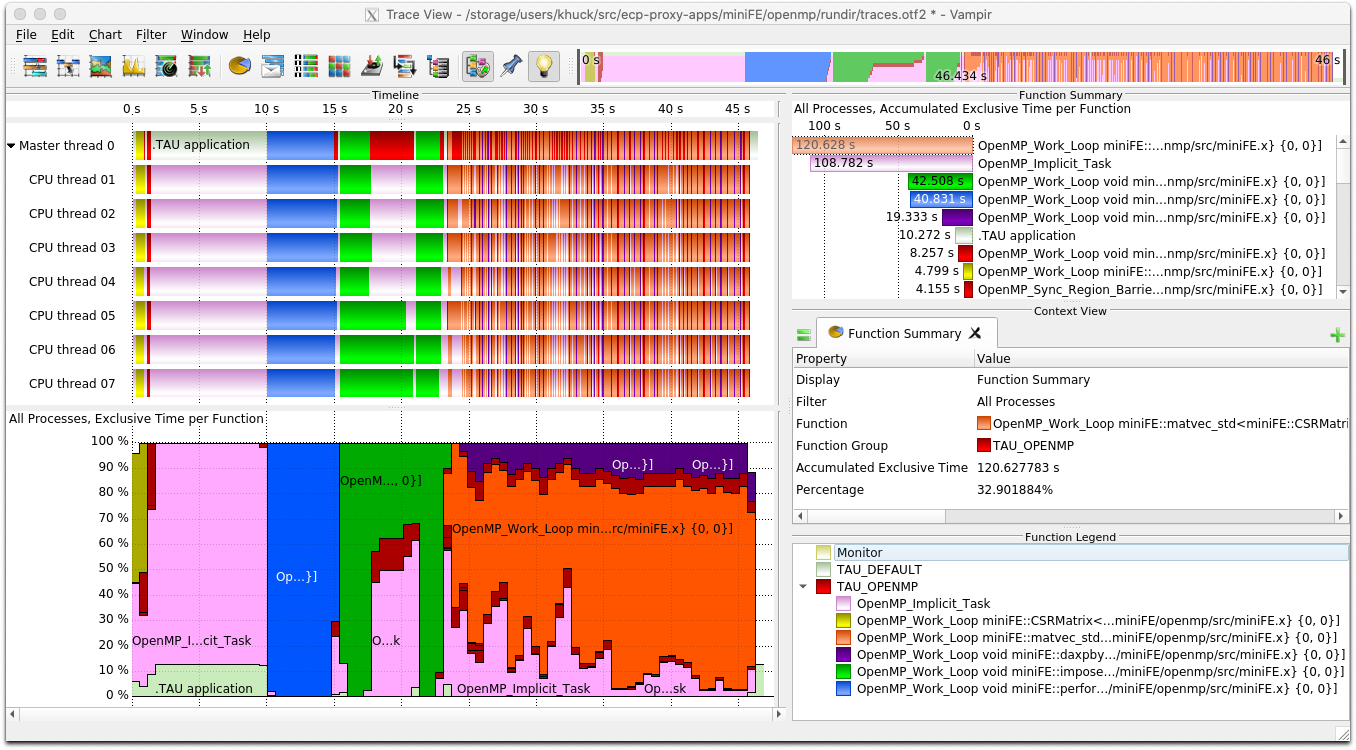
\includegraphics[width=6in]{projects/2.3.2-Tools/2.3.2.10-PROTEAS-YTUNE/miniFE_openmp_tau.png}
\caption{TAU was used to collect profiles and traces of ECP proxy applications like miniFE (shown), observing OpenMP parallel regions, loops and synchronization without application instrumentation.}
\label{figure:tau}
\end{figure}

\begin{figure}[htb]
\centering
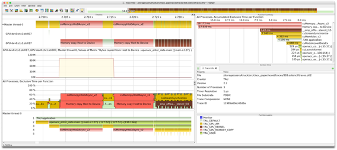
\includegraphics[width=6in]{projects/2.3.2-Tools/2.3.2.10-PROTEAS-YTUNE/clacc_tau.png}
\caption{TAU was used to collect profiles and traces of OpenACC benchmarks (303.stencil shown), observing OpenACC regions and device offload events without application instrumentation.}
\label{figure:tau}
\end{figure}

\paragraph{Recent Progress}
\begin{enumerate}
\item \textbf{Updated CUDA support} Added preliminary support in TAU for NVIDIA A100 GPUs with support for CUDA 11.

\item \textbf{Updated OpenMP support} Updated OMPT support to OpenMP 5.0, tested with ECP Proxy applications miniFE and miniQMC.

\item \textbf{Clacc support} Implemented/updated profiling support for OpenACC events provided by the Clacc compiler.

\item \textbf{HIP} Added support for AMD GPUs with ROCm 3.3.

\item \textbf{CODAR} Updated TAU plugin for streaming profile and trace output to ADIOS2 for realtime application monitoring.  Integrated with Chimbuko framework for runtime trace analysis, demonstrated with XGC on Summit using 768 MPI ranks. (publication accepted to ISAV Workshop @SC20)

\item \textbf{E4S} Integrated TAU in E4S to support AMD GPUs. Both Docker and Singularity images posted on E4S.io website include TAU with support for NVIDIA and AMD GPUs.

\item \textbf{Kokkos} Updated support for Kokkos profiling interface in TAU (publication accepted to ProTools Workshop @SC20).

\item \textbf{LLVM Instrumentation} Implemented an LLVM module for selective instrumentation of C/C++ using TAU, tested with LLVM versions 6 through 12 and Clacc.

\item \textbf{CCAMP} Extended OpenACC and OpenMP interoperable framework, (publication to be presented at SC20).
\end{enumerate}

\paragraph{Next Steps}
\begin{enumerate}
\item \textbf{CUDA Enhancements} 
Implement new Profiling API and Perfworks Metrics API for CUDA/CUPTI 10+.

\item \textbf{OpenMP and OpenACC Enhancements} 
Explore and implement prototype measurement for OpenMP and OpenACC regions executed on target devices.

\item \textbf{New Architectures} 
We plan to support Intel OneAPI with Level Zero and the HPE Cray platform with AMD GPUs.

\item \textbf{Outreach}
Continued outreach activities to demonstrate comprehensive performance evaluation support in TAU for OpenARC, OpenACC, LLVM compiler-based instrumentation, CUDA, Kokkos, ROCm, and NVM based programming frameworks for SHC platforms. 

\item \textbf{E4S} 
Continued integration of TAU and PROTEAS-TUNE projects in the E4S. 

\item \textbf{LLVM Instrumentation} Add Fortran support for LLVM selective instrumentation module, add OpenACC profiling support for F18.

\item \textbf{TAU Instrumentation} Modernize TAU source-to-source auto-instrumentation support in TAU for C++ by replacing current parser front-end with LLVM based solution.

\end{enumerate}

\subsubsection{\stid{2.10} PROTEAS-TUNE - PAPYRUS: Parallel Aggregate Persistent Storage}\label{s:papyrus}

\paragraph{Overview}
Papyrus is a programming system that provides features for scalable, aggregate, persistent memory in an extreme-scale system for typical HPC usage scenarios. Papyrus provides a portable and scalable programming interface to access and manage parallel data structures on the distributed NVM storage. Papyrus allows the programmers to exploit large aggregate NVM space in the system without handling complex communication, synchronization, replication, and consistency models. Papyrus consists of three components, virtual file system (VFS)~\cite{Kim:2017:DIP}, C++ template container library (TCL)~\cite{Kim:2017:DIP}, and key-value store (KV)~\cite{Kim:2017:PHP}.
%Figure~\ref{fig:papyrus-fig} illustrates the overview of Papyrus.
(1) PapyrusVFS provides a uniform aggregate NVM storage image for the different types of NVM architectures. It presents an illusion of a single large NVM storage for all NVM devices available in the distributed system. Unlike other traditional kernel-level VFSs, PapyrusVFS is a lightweight user-level VFS, which is provided as a library so that applications can link to or dynamically load it. PapyrusVFS implements a subset of POSIX API related to file I/O. (2) PapyrusTCL provides a high-level container programming interface whose data elements can be distributed to multiple NVM nodes. PapyrusTCL provides three containers, including map, vector, and matrix, implemented as C++ templates. PapyrusTCL is built on top of PapyrusVFS. This enables PapyrusTCL to be decoupled from a specific NVM architecture and to present a high-level programming interface whose data elements are distributed across multiple NVM nodes transparently. (3) PapyrusKV is a novel embedded KVS implemented specifically for HPC architectures and applications to provide scalability, replication, consistency, and high performance, and so that they can be customized by the application. It stores keys and values in arbitrary byte arrays across multiple NVMs. PapyrusKV provides configurable consistency technique controlled by the application during the program execution dynamically to meet application-specific requirements and/or needs. It also supports fault tolerance and streamlined workflow by leveraging NVM's persistence property.

%\begin{figure}[htb]
%    \centering
%    \includegraphics[width=5in]{papyrus-fig}
%    \caption{\label{fig:papyrus-fig}Papyrus consists of three components, virtual file system, C++ template containers, and key-value store}
%\end{figure}

\paragraph{Key Challenges}
In HPC, NVM is quickly becoming a necessary component of future systems, driven, in part, by the projections of very limited DRAM main memory per node and plateauing I/O bandwidth. More concretely, recent DOE systems, such as NERSC's Cori, LANL/Sandia's Trinity, LLNL's Sierra, OLCF's Summit, TACC's Stampede2, and ALCF's Theta, include some form of NVM. This NVM will be used in two fundamental ways. First, it will be used as a cache for I/O to and from the traditional HDD-based external parallel file systems. In this case, most scientists believe that the caching can be implemented transparently, shielding complexity from the applications and users. Second, NVM will be used as an extended memory to provide applications with access to vast amounts of memory capacity beyond what is feasible with DRAM main memory. More interestingly, in HPC, this extended memory can be aggregated into a much larger, scalable memory space than that provided by a single node alone. In this second case, however, no portable and scalable programming systems exist.

\paragraph{Solution Strategy}
We describe our key goals for Papyrus: high performance, scalability, portability, interoperability with existing programming models, and application customizability. First, \textbf{high performance} is a clear need in HPC. The design of Papyrus should provide the opportunity to exploit NVM resources efficiently. Second, \textbf{scalability} is important in HPC as most of the applications must run on large sectors of the systems - thousands to hundreds of thousands of processors. Papyrus should not inhibit scalability; it should provide an interface that is able to scale as the application and system do. Third, \textbf{portability} is a necessary requirement because HPC applications must be able to run on multiple, diverse platforms at any given time. The upcoming DOE systems all have NVM integrated into the systems in different ways. Papyrus must provide both functional portability and performance portability across systems with different architectures. Fourth, \textbf{interoperability} is a practical requirement of HPC applications. Papyrus must be designed so that it can be incrementally introduced into an application without conflicting with existing HPC programming models and languages like MPI, UPC, OpenMP, OpenACC, C, C++, and Fortran. Furthermore, Papyrus should leverage characteristics of these other programming models when possible. Interoperability allows programmers to adopt Papyrus incrementally in legacy MPI applications avoiding major rewrites of the application. Fifth, \textbf{application customizability} is a key requirement to achieve high performance and scalability. HPC applications have many different usage scenarios, and thus Papyrus should have customizable parameters for key features that impact other important properties like performance and scalability.

\paragraph{Recent Progress}

%Meraculous~\cite{Georganas:2014:PDB} is a state-of-the-art de novo assembler written in UPC. Its parallel algorithm for de Bruijn graph construction and traversal leverages the one-sided communication in UPC to facilitate the requisite random access pattern in the global de Bruijn graph. The de Bruijn graph is implemented as a distributed hash table with an overlapping substring of length {\it k}, referred to as a {\it k-mer}, as key and a two-letter code [ACGT][ACGT] as value as shown in \autoref{fig:papyrus-meraculous}(a). A hash function is used to define the affinities between UPC threads and hash table entries. We ported the distributed hash table written in UPC to a PapyrusKV database. The keys in the database are k-mers and the values are two-letter codes. The PapyrusKV runtime calls the same hash function in the UPC application to determine the owners of key-value pairs in the database by specifying the custom hash function when the database is created. Thus, the thread-data affinities in UPC and PapyrusKV are the same as shown in \autoref{fig:papyrus-meraculous}(a). PapyrusKV requires fewer lines of source code than UPC because it calls standard put and get API functions without implementing an application-specific algorithm for the distributed hash table construction and traversal. \autoref{fig:papyrus-meraculous-eval}(b) shows the performance comparison between PapyrusKV and UPC of Meraculous on Cori. Both versions are built and run using Berkeley UPC, an MPI-interoperable UPC implementation. We measured the total execution time on 32, 64, 128, 256, and 512 UPC threads (32 UPC threads per node). UPC shows better performance than PapyrusKV due to its RDMA capability and built-in remote atomic operations during the graph traversal. The performance gap between UPC and PapyrusKV decreases as the number of UPC threads increases. On 512 UPC threads, PapyrusKV runs 1.5 times slower than UPC. This is mainly because of the asynchronous migration in PapyrusKV during the graph construction.

%\begin{figure}[htb]
%\centering
%\includegraphics[width=3in]{projects/2.3.2-Tools/2.3.2.09-PROTEAS/papyrus-meraculous}
%\caption{K-mer distributed hash table implementations in UPC and PapyrusKV.}
%\label{fig:papyrus-meraculous}
%\end{figure}
%
%\begin{figure}[htb]
%\centering
%\includegraphics[width=3in]{projects/2.3.2-Tools/2.3.2.09-PROTEAS/papyrus-meraculous-eval}
%\caption{Meraculous performance comparison between PapyrusKV (PKV) and UPC on Cori.}
%\label{fig:papyrus-meraculous-eval}
%\end{figure}


%\begin{figure}[t]
%    \centering
%    \begin{minipage}[t]{.48\textwidth}
%        \centering
%        \includegraphics[width=\textwidth]{projects/2.3.2-Tools/2.3.2.10-PROTEAS-YTUNE/papyrus-meraculous}
%        \\(a)
%    \end{minipage}
%    \hfill
%    \begin{minipage}[t]{.48\textwidth}
%        \centering
%        \includegraphics[width=\textwidth]{projects/2.3.2-Tools/2.3.2.10-PROTEAS-YTUNE/papyrus-meraculous-eval}
%        \\(b)
%    \end{minipage}
%    \caption{Using PapyrusKV for Meraculous.
%    (a) K-mer distributed hash table implementations in UPC and PapyrusKV.\label{fig:papyrus-meraculous}
%    (b) Meraculous performance comparison between PapyrusKV (PKV) and UPC on Cori.\label{fig:papyrus-meraculous-eval}}
%\end{figure}

%\begin{figure}[t]
%    \centering
%    \begin{subfigure}[b]{0.45\textwidth}
%        \includegraphics[width=.99\textwidth]{projects/2.3.2-Tools/2.3.2.09-PROTEAS/papyrus-meraculous}
%        \caption{K-mer distributed hash table implementations in UPC and PapyrusKV.}
%        \label{fig:papyrus-meraculous}
%    \end{subfigure}
%    \hfill
%    \begin{subfigure}[b]{0.45\textwidth}
%        \includegraphics[width=.99\textwidth]{projects/2.3.2-Tools/2.3.2.09-PROTEAS/papyrus-meraculous-eval}
%        \caption{Meraculous performance comparison between PapyrusKV (PKV) and UPC on Cori.}
%        \label{fig:papyrus-meraculous-eval}
%    \end{subfigure}
%    \caption{Using PapyrusKV for Meraculous.}
%\end{figure}

%This past year, we have added data compression and encryption to Papyrus. For data compression, the overhead of data access and movement becomes a serious bottleneck compared to compute overhead in large-scale HPC systems. We integrated data compression methods into Papyrus to achieve storage reduction and performance improvement.
%For data encryption, we need to protect sensitive data (e.g., health records, DNA data) that is being used in distributed infrastructures, and users need practical methods to secure their data throughout its lifecycle. We will introduce data encryption in Papyrus to add an extra layer of security in the complex scientific workflows.

\begin{enumerate}
\item \textbf{Data compression and encryption}
  Added data compression and encryption to Papyrus~\cite{Kim:2019:IED}.
  Our compression technique exploits deep memory hierarchy in an HPC system to achieve both storage reduction and performance improvement.
  Our encryption technique provides a practical level of security and enables sharing of sensitive data securely in complex scientific workflows with nearly imperceptible cost.
\item \textbf{Redesign}
  Redesigned and optimized Papyrus to support multidimensional tables.
\item \textbf{Summit}
  Performed preliminary evaluation on OLCF's Summit supercomputer.
\end{enumerate}

\paragraph{Next Steps}

\begin{enumerate}
\item \textbf{Versioning} Versioning can be used to provide new levels of reliability and performance optimization. We will design and implement versioning in Papyrus.

\item \textbf{Performance optimization} New APIs and hardware support is being developed for NVM technologies; we are implementing optimizations in Papyrus to take advantage of these advances.

\end{enumerate}

\newpage
\subsubsection{SOLLVE}\label{subsubsect:sollve}

%% {\itshape
%% 
%% 	\begin{enumerate}
%% 	\item Rename this file to your project WBS-projectname.tex, for example 2.3.3.01-XSDK4ECP.tex.
%% 	\item Complete this template for your project.  Limit your text to two pages, not counting citations.  
%% 	\item Please avoid changing the content of main.tex.  
%% 	\item Put any references in a .bib file with the same root name, for example 2.3.3.01-XSDK4ECP.bib.
%% 	\item Remember to include any image files you reference in your text.
%%     \item The files 2.3.3.01-XSDK4ECP.tex, 2.3.3.01-XSDK4ECP.bib and xSDK-diagram.jpeg are included as examples for your reference.  You can remove them from what you upload.
%% 	\end{enumerate}
%% }


\paragraph{Overview}
OpenMP is a directive-based API for intra-node programming that is widely used  in ECP applications. Implementations of OpenMP and  tools to facilitate OpenMP application development.are available in all DOE LCFs.  
The specification is supported by a stable community of vendors, research labs, and academics who
participate in the efforts of the  OpenMP Architecture Review Board (ARB) and its Language Committee to evolve its features.
The mission of the SOLLVE project is to further enhance  OpenMP and its implementations to meet the performance and productivity goals of ECP applications. 

SOLLVE has identified open ECP application software requirements, developed features and/or implementation technology to address them, and created use cases that motivate the need for enhancements. 
 The project continues to identify needs and works to standardize them via 
%In addition to 
active participation in the deliberations of the Language Committee.  
%SOLLVE has moreover produced 
% prototype
%implementations of key new features to support their rapid adoption.

The project is  developing a verification and validation (V\&V) suite to assess implementations and
enable evaluations by DOE  facilities. It is constructing a high-quality,  robust 
OpenMP implementation based on the LLVM compiler. 
%%% BC put in suitable place: resolution of various interoperability 
 SOLLVE plays a critical
role in specifying, implementing, promoting, and deploying functionality
that will enable ECP application developers to reach their goals using OpenMP.
%The project will demonstrate the high impact of new features via their use in selected
%ECP applications.

\paragraph{Key  Challenges}
%\textit{Describe what is hard to do, why it is challenging.}
%need more features, need more implementations (with quality)
Gaps in OpenMP functionality exist as a result of the rapid evolution of node architectures and  base programming languages, as well as a lack of focus on performance portability before version 5.0.  
 Since vendor representatives dominate the  OpenMP Language Committee, effort is needed  to secure their support with regard to the scope of the API, as well as  the syntax and semantics of new features.

%large feature set, many new features are important for ECP
The API has greatly expanded in recent years as some of these gaps are closed, placing a large burden on its implementers. 
The timely provision of  robust implementations of new features that are critical for ECP is therefore particularly challenging.
%%Must we delete this line?
For performance portability, consistent approaches in multiple implementations is highly desirable. Interoperability concerns have emerged as a  new challenge.
 
 %need help to get good performance. 

Given the lack of availability of implementations with features that target accelerators, many existing codes have used alternative APIs for GPUs: a significant effort will be required to replace those approaches by OpenMP. A broad effort is required to develop and apply best practices for new features and platforms. 

\paragraph{Solution Strategy}
We address the challenges by focusing on the following primary activities:

\begin{enumerate}
\item {\bf Application requirements}
Ongoing in-depth interactions with selected ECP application teams have resulted in a list of required extensions, some of which have been met by the recent 5.0 specification.  New needs are being identified. This work informs all other project activities by producing use cases, detailed feedback and example codes. It moreover contributes to the OpenMP Examples document. 
\item {\bf OpenMP specification evolution}
Members of the SOLLVE project are active participants in the OpenMP Language committee.  The project creates early prototypes for new features based on ECP use cases, develops concrete proposals and submits them for standardization. Several proposed features  were included in OpenMP 5.0, ratified November 2018. More are under development for version 5.1.
\item {\bf LLVM  Compiler}
SOLLVE implements new OpenMP features in the LLVM compiler and develops analyses and transformations that enhance, and provide consistency to, OpenMP performance. Its open source solutions may be leveraged in vendor compilers.
The compiler is available on LCF platforms.
\item {\bf Lightweight OpenMP runtime}
The BOLT runtime, built upon ultra-lightweight threading, addresses the need for efficient nested parallelism and improved task scheduling, it develops better support for interoperability with MPI. BOLT is integrated and delivered with the project's LLVM compiler. 
\item {\bf Validation and Verification (V\&V)} 
A V\&V suite is being implemented that allows vendors, users and facilities to assess the coverage
and standard compliance of OpenMP implementations. A ticket system for bug reporting and inquiries has also been deployed to facilitate interaction with end users.
\item{\bf Training and Outreach}
 Tutorials and webinars are delivered to provide information on OpenMP features and their usage, as well as updating on the status of  %their support in vendor and open source 
 implementations. Deeper interaction with application programmers via hackathons supports the development of ECP codes using all available OpenMP features.
%  also provides immediate feedback to compiler and tool developers as the application teams experiment with the use of new features.  
\end{enumerate}
%%revision needed starting here: publications from IWOMP, Lingda, etc.


\paragraph{Recent Progress}
Figure \ref{fig:sollve-update} shows the latest progress on the 5 core SOLLVE
thrust areas. The {\bf training and outreach} activity is a
cross-cutting effort which is supported by resources from SOLLVE and  ECP Broader Engagement,
 with contributions by external collaborators, notably Lawrence Berkeley National
Laboratory.   
%Oak Ridge and Delaware are not external so I commented this out in the hope it can benefit the figure
%project and
%external partners, namely collaborators from Lawrence Berkeley National
%Laboratory, Oak Ridge, University of Delaware and other academic institutions.
A number of articles have also been published
as part of the SOLLVE
effort~\cite{openmp-tr6,zinenko.cc.2018,vandv2019,
tregion, Mishra:2019:KFA:3314872.3314915,
udm, loopTransPragmas, DBLP:conf/iwomp/SreenivasanJHBS19,
DBLP:conf/iwomp/ScoglandSOHES19, DBLP:conf/iwomp/0001WLSS19,
DBLP:conf/iwomp/KaleIKKC19, Bak2019OptimizedEO, lsrt, boltPACT19}.


%% The value that SOLLVE brings to ECP is observed in the ease of leveraging
%% different OpenMP features related to data mappings, parallelism exposure (e.g.
%% {\bf concurrent} or {\bf simd} directives) and control (affinity), runtime
%% scheduling and accelerator (device) offloading (e.g. GPUs or FPGAs).

\begin{figure}[t]
\includegraphics[width=1.0\linewidth,height=9.1cm]{projects/2.3.2-Tools/2.3.2.11-SOLLVE/SOLLVE-progress}
\caption{\label{fig:sollve-update}SOLLVE thrust area updates}
\end{figure}
%\textit{Describe what you have done recently.  It would be good to have some kind of figure or diagram in this section.}

\paragraph{Next Steps}
The following next steps are planned:
\begin{itemize}
\item Applications: Continue to interact with ECP applications teams, evaluate implementations of new features and explore new requirements; identify best practices for the use of OpenMP on accelerators;

\item OpenMP specification: Continue work toward the next version of the standard via ECP-motivated feature development and participation in the OpenMP Language Committee: version 5.1 is underway and due for release November 2020;

\item LLVM compiler: Improve performance of device offloading and optimize generation of code within target devices; generalize to enable reuse across multiple offloading architectures; develop infrastructure to support integration of Fortran front end; increase parallel region performance; implementation of OpenMP 5.1 loop transformations;

\item  OpenMP runtime: Provide support for 5.0 spec; investigate performance optimization of MPI+OpenMP codes; address broader set of interoperability challenges; address advanced tasking requirements; 

\item V&V suite: Continue expanding the coverage of the V&V Suite, with focus on 5.0 features and additions and corrections to 4.5 tests as OpenMP implementations mature; expand Fortran tests; work with ARB Examples Committee; improve ALCF toolchains; more vendor interactions.
\end{itemize} 



%\textit{Describe what you are working on next.}

%\item Applications: Continue to interact with ECP applications teams, evaluate implementations of new features and explore new requirements; 
% create mini-apps to help evaluate OpenMP accelerator support; 
 %identify best practices for the use of OpenMP on accelerators;
%for memory management API and concurrent parallel construct; prepare and coordinate %OpenMP webinar focusing on memory management, deep copy and tasking. Spack %package development and deployment with applications. 
%\item OpenMP specification: Continue work toward the next version of the standard via ECP-motivated feature development and participation in the OpenMP Language Committee: version 5.1 is already well under way and is due for release November 2020;
%Next face-to-face meeting in January 2019; ratify and vote latest memory management %features and mappers, vote on examples, add to loop scheduling and tasking for affinity %research. 
%\item LLVM compiler: Improve performance of device offloading and optimize generation of code within target devices; generalize to enable reuse across multiple offloading architectures; develop infrastructure to support integration of Fortran front end; increase parallel region performance; 
%develop new optimizations for loop transformations; refine Clang based implementation of data layout transformations for OpenMP offloading; improve general testing; evaluate on Summit and other ECP systems. 
%\item OpenMP runtime: provide support for 5.0 spec; improve performance of MPI+OpenMP codes; address broader set of interoperability challenges; address advanced tasking requirements;
% and MPI implementations
%\item V\&V suite: Continue expanding the coverage of the V\&V Suite, with main focus on 4.5 features;  expand Fortran tests; work with ARB Examples Committee; improve ALCF toolchains;
%\end{itemize}


\subsubsection{\stid{2.11} Argobots: Flexible, High-Performance Lightweight Threading }

\paragraph{Overview}

Efficiently supporting massive on-node parallelism demands highly
flexible and lightweight threading and tasking runtimes. At the
same time, existing lightweight abstractions have shortcomings while
delivering generality and specialization.  Our group at Argonne
developed a lightweight, low-level threading and tasking framework,
called Argobots.  The key focus areas of this project are: (1) To
provide a framework that offers powerful capabilities for users to
allow efficient translation of high-level abstractions to low-level
implementations. (2) To provide interoperability with other
programming systems such as OpenMP and MPI as well as with other
software components (e.g., I/O services). (3) To provide a programming
framework that manages hardware resources more efficiently and reduce
interference with co-located applications.

\paragraph{Key Challenges}

Several user-level threading and tasking models have been proposed in
the past to address the shortcomings of OS-level threads, primarily
with respect to cost and flexibility. Their lightweight nature and
flexible generic interface play an important role at managing
efficiently the massive concurrency expected at the Exascale level.
Existing user-level threading and tasking models, however, are either
too specific to applications or architectures or are not powerful or
flexible. Existing runtimes tailored for generic use \cite{GNUPth,
PLDI97_Taura, COSET05_Thibault, COB14_Nakashima, MTAAP08_Wheeler,
PPoPP99_Taura, SenSys06_Dunkels, TBB1, EuroPar08_Perache} are suitable
as common frameworks to facilitate portability and interoperability
but offer insufficient flexibility to efficiently capture higher-level
abstractions, while specialized runtimes \cite{ATC02_Adya,
SolarisThreads, SOSP03_von_Behren, StateThreads, PLDI07_Li,
MTAAP09_Porterfield, WMPP05_Cuvillo, IntelOMP, Nanos++, LCPC96_Kale,
PACT14_Treichler} are tailored to specific environment.

\paragraph{Solution Strategy}

Argobots offers a carefully designed execution model that balances
generality of functionality with providing a rich set of controls to
allow specialization by end users or high-level programming models
\cite{seo2018}.  Delivering high performance in Argobots while
providing a rich set of capabilities is achieved by heavily optimizing
critical paths as well as by exposing configuration knobs and a rich
API, which allow users to trim unnecessary costs. Furthermore,
Argobots honors high degrees of expressibility through the following
three key aspects:

\begin{enumerate}

\item Capturing the requirements of different \emph{work units}, which
are the most basic manageable entities. Work units that require
private stacks and context-saving capabilities, referred to as
\textit{user-level threads} (ULTs, also called \textit{coroutines} or
\textit{fibers}), are fully fledged threads usable in any context.
\emph{Tasklets} do not require private stacks. They are more
lightweight than ULTs because they do not incur context saving and
stack management overheads.  Tasklets, however, are restrictive; they
can be executed only as atomic work units that run to completion
without context switching.

\item Exposing hardware computational units through \emph{execution
streams} (ESs) as OS-level threads to execute work units. Unlike
existing generic runtimes, ESs are exposed to and manageable by users.

\item Allowing full control over \emph{work unit management}.  Users
can freely manage \emph{scheduling} and mapping of work units to ESs
through \emph{thread pool} management, and thus achieving the desired
behavior. Figure~\ref{fig:sollve-argobots} illustrates the various
building blocks in the Argobots framework and the interactions between
them to build a hypothetical system.

\end{enumerate}

\begin{figure}[htb]
  \centering
  \includegraphics[height=3in]{projects/2.3.2-Tools/2.3.2.11-SOLLVE/SOLLVE-ARGOBOTS.pdf}
  \caption{\label{fig:sollve-argobots}Argobots execution model}
\end{figure}

\paragraph{Recent Progress}

Threading overheads are crucial for fine-grained parallel applications
and runtimes running in massively parallel environments.  We have
found that the timing of yield operations highly affects the
performance of lightweight threads~\cite{iwasaki2018}, but other
factors remained unexplored.  We further optimized fork-join overheads
by exploring new threading methods with respect to stack allocation
timing and scheduling policies and a wider range of modern hardware
architectures.  Our evaluation shows that our child-first scheduling
yields promising results for deep and narrow recursive task-parallel
programs while the parent-first scheduling is good for flat
parallelism.  Our study helps users and application developers choose
the best threading methods that fit their hardware architectures and
application workloads and maximize the scalability~\cite{iwasaki2020}.

Integration with other runtime systems is fundamentally important for
the Argobots project.  BOLT, a SOLLVE OpenMP runtime over
Argobots~\cite{BOLT}, is one of the most successful parallel
programming systems using Argobots.  Our enhancements of Argobots
threads lowers the cost of OpenMP threading and tasking.  The Argobots
project continues to improve interoperability with communication
layers such as MPI runtimes (e.g., MPICH and Open~MPI) and Margo, a
Mercury RPC over Argobots.  To help their performance analysis, our
latest Argobots 1.1a1 release includes a lightweight yet powerful
profiling interface, which helps runtime developers pinpointing a
performance problem in these systems.  I/O service is one of the most
important application areas for Argobots. Intel DAOS, a next-
generation high-performance storage system developed by Intel, uses
Argobots to efficiently handle asynchronous I/O messages.  We are
working together to improve Argobots by providing a better debugging
interface such as stack dump features. Our CI testing has been
extended for various CPU architectures, operating systems, and
compilers to cover most of the DOE HPC platforms.  Thanks to our CI,
Argobots 1.1a1 works on major UNIX-based platforms including Ubuntu,
FreeBSD, CentOS, macOS, and Solaris. Argobots supports most CPU
architectures with special optimizations for Intel/AMD x86/64,
ARMv8-A, and POWER 8 and 9. Argobots can be compiled with numerous C
compilers including GCC, Clang, ICC (Intel), XLC (IBM), PGCC (PGI),
Solaris Studio (Oracle), and Arm C Compiler for HPC (ARM).

The innovative design and implementation of Argobots are highly
recognized.  Argobots was named a finalist for the 2020 R\&D 100
Awards.  The prestigious R\&D 100 competition, sponsored by R\&D
Magazine, recognizes the 100 most innovative technologies of the
previous year.  Argobots, a lightweight and highly flexible
multithreading framework, was chosen as a finalist for the 2020 R\&D
100 Awards.

\paragraph{Next Steps}

Argobots continues to implement new features and optimizations for
application needs, while our substantial efforts will be made to
promote integration and composition with other systems. Our major
ongoing and planned steps are as follows.

\begin{enumerate}

\item Further integration with other applications and runtimes
including MPI runtimes including MPICH and Open MPI.  In collaboration
with MPICH and Open MPI developers, we will further optimize their
Argobots interoperability layers by utilizing user-level threading
techniques.

\item Enhanced interoperability of multiple components that are not
aware of Argobots.  Unfortunately, not all applications are written
for lightweight ULTs; some programs suffer from core starvation and,
in the worst case, deadlocks if they are running on Argobots.  To
address this issue, we are investigating an approach that is as
lightweight as the current Argobots ULTs while it has the OS-implicit
preemption functionality that traditional OS-level threads have.

\end{enumerate}

\subsubsection{\stid{2.11} BOLT: Lightning Fast OpenMP}\label{subsubsect:bolt}

\paragraph{Overview}

OpenMP is central for several applications that target Exascale,
including ECP applications, to exploit on-node computational
resources.  Unfortunately, current production OpenMP runtimes, such as
those that ship with Intel and GNU compilers, are inadequate for the
massive and fine-grained concurrency expected at the Exascale level.
These runtimes rely on heavy-handed OS-level threading strategies that
incur significant overheads at fine-grained levels and exacerbate
interoperability issues between OpenMP and internode programming
systems, such as MPI and OpenSHMEM.  BOLT is a production quality
OpenMP runtime (called BOLT) which has been developed within the
SOLLVE project to address this issue by leveraging user-level threads
instead of OS-level threads (e.g., Pthreads).  Due to their
lightweight nature, managing and scheduling user-level threads incurs
significantly less overheads.  Furthermore, interoperability between
BOLT and internode programming systems opens up new optimization
opportunities by promoting asynchrony and reducing hardware
synchronization (atomics and memory barriers).  Initial studies on
this proposal can be found in \cite{amer2018, ccgrid, ppopp}. This
report briefly summarizes the issues in OpenMP runtimes that rely on
OS-level threading, describes BOLT as the solution to this challenge,
the current status in the BOLT effort, and the next steps for further
improvements.

\paragraph{Key Challenges}

The growing hardware concurrency in High Performance Computing (HPC)
cluster nodes is pushing applications to chunk work more fine-grained
to expose parallelism opportunities.  This is often achieved through
nested parallelism either in the form of parallel regions or by
explicit tasks.  Nested parallel regions can potentially cause
oversubscription of OS-level threads to CPUs and thus lead to
expensive OS-level thread management.  Such heavy costs usually
outweigh the benefits of increased concurrency and thus compel the
OpenMP programmer to avoid nested parallel regions altogether.  Such
workaround, however, not only causes poor resource utilization from
insufficient parallelism but is also not always possible.  For
instance, the nested level could be outside the control of the user
because it belongs to an external library that also uses OpenMP
internally.  Internode programming systems, such as MPI and OpenSHMEM,
are not aware of OpenMP semantics, such as the notion of an OpenMP
task.  What these internode systems understand is the low-level
threading layer used by OpenMP, such as Pthreads.  This threading
layer serves as the interoperability medium between OpenMP and the
internode programming system and has a direct impact on performance.
It is notoriously known that OS-level thread safety in production MPI
libraries suffers significant performance issues. While continued
progress on improving OS-level thread safety in these important
internode programming systems is crucial for traditional
interoperability, we propose in this work exploring an orthogonal
direction that assumes a more lightweight interoperability layer.

\paragraph{Solution Strategy}

Both fine-grained parallelism and interoperability issues suffer from
the heavy nature of working at the level of OS threads.  Our solution
to both challenges leverages user-level threads.  Using user-level
threads as the underlying threading layer for the OpenMP runtime
offers a significantly better trade-off between high concurrency and
thread management overheads.  This allows users to generate
fine-grained concurrency and oversubscription without worrying about
the performance collapse that is observed in current OpenMP runtimes.
Our OpenMP runtime, BOLT, is derived from the LLVM OpenMP runtime and
leverages Argobots, a highly optimized lightweight threading library,
as its underlying threading layer.  OpenMP threads and tasks are
spawned as Argobots work units and nested parallel regions are managed
through an efficient work-stealing scheduler.  Furthermore, new
compiler hints and runtime optimizations have been developed to allow
reducing thread management overheads even further~\cite{iwasaki2018,
iwasaki2020}. Interoperability improvements have also been
demonstrated by having BOLT interoperate with an MPI libraries through
the Argobots threading layer rather than OS-level threads.  Results
showed that this approach allows better communication progress and
outperforms the traditional Pthreads-level interaction~\cite{seo2018}.

\paragraph{Recent Progress}

\begin{figure}[t]
  \centering
  \includegraphics[width=0.9\columnwidth]{projects/2.3.2-Tools/2.3.2.11-SOLLVE/SOLLVE-BOLT.pdf}

  \caption{\label{fig:sollve-bolt} MPI+Threads interoperability of
  BOLT.  OpenMP threads and tasks in BOLT interact MPI implementations
  via the Argobots layer.}
\end{figure}

We improved the interoperability of BOLT with various MPI systems via
lightweight threads, Argobots.  Since most MPI runtimes including
MPICH, Open~MPI, and production MPI implementations that are derived
from either MPICH or Open~MPI assume OS-level threads as ``Thread'' in
MPI+Thread, lightweight OpenMP runtimes based on lightweight threads
failed to interoperate well with existing MPI systems.  To address
this issue, we have implemented an abstracted threading layer for
lightweight threads in these MPI runtimes so that users can choose
OpenMP threads and tasks of BOLT as ``Thread''.

Specifically, we focused on the MPI interoperability with the most
widely used open-source MPI implementations: MPICH and Open~MPI.  For
MPICH, we fixed a few bugs regarding synchronization mechanisms, which
will be included in the MPICH 3.4 release.  In collaboration with the Open MPI
researchers and the Qthreads researchers at Sandia and Los Alamos
National Laboratories, we implemented a new thread abstraction layer
for generic threading runtime support in Open~MPI using the Opal
Modular Component Architecture.  This highly abstracted threading
layer has been implemented carefully to minimize the additional
overheads.  Furthermore, this Opal architecture partly allows the
programmer to choose an underlying threading library at compile- or
run-time to provide flexibility.  The performance trade-off has
been discussed in our work~\cite{ExaMPI20MCAThreads}.  This Open MPI
interoperability improvement will be included in the Open~MPI 5.0
release. To ensure availability, we employed a weekly CI testing
infrastructure for those MPI systems.

Our latest BOLT 1.0 release contains a large upgrade to be compatible
with LLVM OpenMP 10.0, which further improves performance and
functionalities especially for GPU offloading and new OpenMP 5.0
features.  This release also contains scheduler improvement in BOLT
and an upgrade of the Argobots package, which allows further
lightweight fine-grained OpenMP threading and tasking.  Interaction
and integration are a critical piece for the BOLT project.  We
continue working on the SOLLVE Spack package so that this BOLT system
is available on our target HPC systems and users can utilize BOLT for
(1) ECP applications that have fine-grained parallelism such as nested
parallel regions and tasking (e.g., ECP SLATE) and (2) runtime systems
via the Argobots layer (such as MPICH and Open MPI we mentioned) that
can take advantage of ULT's lightweight synchronization for resource
management.

\paragraph{Next Steps}

One of the largest advantages of BOLT is an underlying lightweight
thread implementation, flexible scheduling, and high interoperability
thanks to Argobots. The following list includes our next plans:

\begin{enumerate}

\item Explores opportunities for utilizing lightweight threads for
other optimizations in the context of OpenMP.  The main focus of BOLT
has been the performance of fine-grained OpenMP threads, so we have
not fully explored how BOLT could elevate the performance of other
parallel units (e.g., data-dependent tasking and GPU offloading). We
are planning to investigate room for optimizations and implement them
with evaluation.

\item Investigates the performance with large-scale applications.
In order to find potential room for optimizations and evaluate the
performance of BOLT in real large-scale workloads, we further
investigate other SOLLVE components and ECP applications that can benefit from BOLT.  Since most distributed systems rely on MPI for internode
communication, we will also work on tighter integration with MPI to
optimize the performance with MPI runtimes over BOLT.

\end{enumerate}

\newpage
\documentclass[10pt]{article}
\usepackage[usenames]{color} %used for font color
\usepackage{amssymb} %maths
\usepackage{amsmath} %maths
\usepackage[utf8]{inputenc} %useful to type directly diacritic characters
\begin{document}
\[\subsubsection{\stid{2.12} Flang}\label{subsubsect:flang}

\paragraph{Overview}

The Flang project provides an open source Fortran
\cite{iso-fortran-2004} \cite{iso-fortran-2010} \cite{iso-fortran-2018}
compiler.  The project was formally accepted as a component of the LLVM 
Compiler Infrastructure last year (see \url{http://llvm.org})~\cite{llvm:homepage} 
and has merged portions of its initial codebase into the main 
LLVM repository as of April 2020. Leveraging LLVM, Flang will provide a 
cross-platform Fortran solution available to ECP and the broader 
international LLVM community. The goals of the project include
extending support to GPU accelerators and target Exascale systems, and 
supporting LLVM-based software and tools R\&D of interest to a large 
deployed base of Fortran applications.

LLVM's growing popularity and wide adoption make it an integral part
of the modern software ecosystem. This project provides the foundation
for a Fortran solution that will complement and interoperate with the
Clang C/C++ compiler and other tools within the LLVM infrastructure.
We aim to provide a modern, open-source Fortran implementation that is
stable, has an active footprint within the LLVM community, and will
meet the specific needs of ECP as well as the broader scientific
computing community.

\paragraph{Key Challenges}
Today there are several commercially-supported Fortran compilers,
typically available on only one or a few platforms.  None of these are
open source.  While the GNU gfortran open source compiler is available
on a wide variety of platforms, the source base is not modern
LLVM-style C++ and the GPL open source license is not compatible with
LLVM, both of which can impact broader community participation and adoption.

The primary challenge of this project is to create a source base with
the maturity, features, and performance of proprietary solutions with
the cross-platform capability of GNU compilers, and which is licensed
and coded in a style that will be embraced by the LLVM community.
Additional challenges come from robustly supporting all Fortran
language features, programming models, and scalability required for 
effective use on Exascale systems. 

\paragraph{Solution Strategy}

With the adoption of Flang into the LLVM community, our strategy
focuses on building a strong community around it and the development
and delivery of a solid, alternative Fortran compiler for DOE's
Exascale platforms.  It is critical that we be good shepherds within
the broad LLVM community to successfully establish and grow a vibrant
community for Flang. This external engagement is in the best interest
of ECP as well as the long-term success of Fortran in the LLVM
community and the many industry products that rely upon it.

Our path to success will rely on significant testing across not only
the various facilities but also across a very broad and diverse set of
applications. Given the early development stage of Flang, this testing
will be paramount in the delivery of a robust infrastructure to ECP
and the broader community.

\paragraph{Recent Progress}

After several years of effort and support from NNSA, Flang was 
successfully \emph{``adopted''} by the LLVM community and has transitioned 
from a stand-alone git repository to one hosted by the main LLVM project.  This 
represents a significant result and the current code is available via GitHub:

\begin{center}
\url{https://github.com/llvm/llvm-project/tree/master/flang}
\end{center}

The current capabilities of flang include the full Fortran 2018
standard and OpenMP 5.X syntax and semantics.  As part of the
development of the parsing and semantic analysis portions of the
front-end, over five million lines of Fortran code has been
successfully processed. Beyond parsing and semantics, we have been
focusing our efforts on creating a Fortran-centric intermediate 
representation (Fortran IR -- ``FIR'') that leverages recent activities 
within Google on 
\href{Multi-Level Intermediate Representations} 
{https://www.blog.google/technology/ai/mlir-accelerating-ai-open-source-infrastructure/}
(MLIR) for use with the implementation of FIR.
With the development of FIR progressing, we are approaching completion of 
the first full (sequential) compiler with the full set of F77 
capabilities, and implementations of later standards are expected to 
follow naturally after that.

\paragraph{Next Steps}
Our short-term priorities are focused on the completion of the
sequential compiler, the creation of a significant testing
infrastructure, and helping to lead the interactions and overall
discussions within the LLVM community.  Longer term efforts
will shift to support OpenMP 5.X features critical to ECP applications
on the target Exascale platforms.  We are actively exploring finding a
common leverage point between Clang's current OpenMP code base and
Flang.  This would enable the reuse of existing code versus writing
everything from scratch in Flang.  We see this as a critical path
forward to enabling a timely release of a node-level parallelizing
compiler for ECP.  Additional work will focus on features that would
benefit Fortran within the LLVM infrastructure as well as general and
targeted optimization and analysis capabilities.

\]
\end{document}

\newpage


%\subsection{\mathlibs}
%This section presents projects in \mathlibs.
\subsection{\stid{3} \mathlibs}\label{subsect:mathlibs}

\textbf{End State:} Mathematical libraries that (i) interoperate with the ECP software stack; (ii) are incorporated into the ECP applications; and (iii) provide scalable, resilient numerical algorithms that facilitate efficient simulations on Exascale computers.

\subsubsection{Scope and Requirements}
Software libraries are powerful means of sharing verified, optimized algorithms and their implementations. Applied research, development, and support are needed to extend existing DOE mathematical software libraries to make better use of Exascale architectural features. DOE-supported libraries encapsulate the latest results from mathematics and computer science R\&D; many DOE mission-critical applications rely on these numerical libraries and frameworks to incorporate the most advanced technologies available. 

The Mathematical Libraries effort will ensure the healthy functionality of the numerical software libraries on which the ECP applications will depend. The DOE mathematical software libraries used by computational science and engineering applications span the range from light-weight collections of subroutines with simple APIs to more “end-to-end” integrated environments and provide access to a wide range of algorithms for complex problems.

Advances in mathematical and scientific libraries will be necessary to enable computational science on Exascale systems. Exascale computing promises not only to provide more computational resources enabling higher-fidelity simulations and more demanding studies but also to enable the community to pose new scientific questions. Exascale architectural characteristics introduce new features that algorithms and their implementations will need to address in order to be scalable, efficient, and robust. As a result, it will be necessary to conduct research and development to rethink, reformulate, and develop existing and new methods and deploy them in libraries that can be used by applications to deliver more complete and sophisticated models and provide enhanced predictive simulation and analysis capabilities.

The Mathematical Libraries effort must (1) collaborate closely with the Application Development effort (WBS 2.2) to be responsive to the needs of the applications and (2) collaborate with the other products within the Software Technology effort (WBS 2.3) in order to incorporate new technologies and to provide requirements. All software developed within the Mathematical Libraries effort must conform to best practices in software engineering, which will be formulated early in the project in collaboration with the Applications Development focus area. Software produced by this effort must provide scalable numerical algorithms that enable the application efforts to reach their performance goals, encapsulated in libraries whose data structures and routines can be used to build application software.

\subsubsection{Assumptions and Feasibility}
Years of DOE investment have led to a diverse and complementary collection of mathematical software, including AMReX, Chombo, hypre, Dakota, DTK, MAGMA, MFEM, PETSc/TAO, PLASMA, ScaLAPACK, SUNDIALS, SuperLU, and Trilinos. This effort is evolving a subset of existing libraries to be performant on Exascale architectures. In addition, research and development is needed into new algorithms whose benefits may be seen only at the extreme scale. Results of preliminary R\&D projects indicate that this approach is feasible.

Additionally, ECP will need to rely on a strong, diverse, and persistent base math research program, which is assumed to continue being supported by the DOE-SC ASCR Office. The ECP technical directors will schedule quarterly meetings with the ASCR research program managers to get updates on research results that might meet ECP requirements as well as to inform the program managers of ECP needs in applications and software components.

\subsubsection{Objectives}
The high-level objective of the Mathematical Libraries effort is to provide scalable, resilient numerical algorithms that facilitate efficient application simulations on Exascale computers. To the greatest extent possible, this objective should be accomplished by preserving the existing capabilities in mathematical software while evolving the implementations to run effectively on the Exascale systems and adding new capabilities that may be needed by Exascale applications.

The key performance metrics for the software developed by this effort are scalability, efficiency, and resilience. As a result of the new capabilities in mathematics libraries developed under this effort, applications will tackle problems that were previously intractable and will model phenomena in physical regimes that were previously unreachable.

\subsubsection{Plan}
As detailed below, the Mathematical Libraries effort supports six complementary L4 projects as needed to meet the needs of ECP applications. These efforts include strong collaborations among DOE labs, academia, industry, and other organizations, and leveraging existing libraries that are widely used by the DOE HPC community. 

Initial efforts have focused on identifying core capabilities needed by selected ECP applications, establishing performance baselines of existing implementations on available Petascale and prototype systems, and beginning re-implementation of lower-level capabilities of the libraries and frameworks. Another key activity is collaborating across all projects in the Mathematical Libraries effort to define community policies in order to enable compatibility among complementary software and to provide a foundation for future work on deeper levels of interoperability. Refactoring of higher-level capabilities will be prioritized based on needs of the applications. In time, these efforts will provide demonstrations of parallel performance of algorithms from the mathematical software on pre-Exascale, leadership-class machines (at first on test problems, but eventually in actual applications). The initial efforts also are informing research into advanced exascale-specific numerical algorithms that will be implemented within the libraries and frameworks. In FY20–23, the focus will be on development and tuning for the specific architectures of the selected exascale platforms, in addition to tuning specific features that are critical to ECP applications. The projects will implement their software on the CORAL, NERSC and ACES systems, and ultimately on initial Exascale systems, so that functionality, performance, and robustness can be evaluated by the applications teams and other elements of the software stack. Throughout the effort the applications teams and other elements of the software stack will evaluate and provide feedback on their functionality, performance, and robustness. These goals will be evaluated at least yearly based on milestones as well as joint milestone activities shared across the associated software stack activities by Application Development and Hardware and Integration project focus areas.


\subsubsection{Risks and Mitigations Strategies}
There are a number of foreseeable risks associated with the Mathematical Libraries effort.
\begin{itemize}
	\item Efficient implementation of new or refactored algorithms to meet Exascale computing requirements may introduce unanticipated requirements on programming environments. To mitigate this risk, effective communication is needed between projects in the Mathematical Libraries effort and projects tasked with developing the programming environments. From the application perspective, this is specifically tracked in a specific AD risk the risk register. Additionally, the risks of an inadequate programming environment overall are tracked as a specific ST risk in the risk register.
	\item A significant number of existing algorithms currently implemented in numerical libraries may scale poorly, thereby requiring significantly more effort than refactoring. The R\&D planned for the first three years of the ECP is the first mitigation for this risk (as well as the co-design centers planned in Application Development). In addition, the ECP will be able to draw from a strong, diverse, well-run, persistent base math research program. From the application perspective, this is tracked via an AD risk in the risk register. Scaling issues for the software stack in general, including libraries, are monitored via an ST risk in the risk register.
	\item Exascale architecture characteristics may force a much tighter coupling among the models, discretizations, and solvers employed, causing general-purpose solvers to be too inefficient. The mitigation strategy is to ensure close collaboration with the sub-elements of the Application Development focus area (WBS 2.2) to understand integration and coupling issues. Again, a strong, diverse, well-run, persistent base math research program may provide risk mitigation strategies.
\end{itemize}

\subsubsection{Future Trends}
Mathematical libraries have been one of the strongest success stories in the scientific software ecosystem.  These libraries encode specialized algorithms on advanced computers that can be the difference between success or not.  Algorithms such as multigrid, highly-tuned dense linear algebra and optimized FFTs, can improve performance by orders of magnitude and reduce the asymptotic algorithmic complexity for users.  We foresee that math libraries will have an ever-growing role in the scientific software ecosystem, as architectures become more challenging for targeting optimization and algorithms require even more concurrency and latency hiding in order to realize performance on modern computer systems.

In addition, we anticipate that new algorithms based on multi-precision arithmetic will further enable performance improvements on compute devices that are optimized for machine learning workloads, where short precision can be an order of magnitude faster that double precision.  

For a deeper discussion of the futures of ECP Math Libraries efforts, please consult the paper ``Preparing Sparse Solvers for Exascale Computing''~\cite{ECP-Solvers}.
\newpage
\subsubsection{\stid{3.01} xSDK} 
\paragraph{Overview} The xSDK project is creating a value-added aggregation of DOE math and scientific libraries through the xSDK (Extreme-scale Scientific Software Development Kit)~\cite{xsdk:homepage}, which increases the combined usability, standardization, and interoperability of these libraries as needed by ECP. The project focuses on community development and a commitment to combined success via quality improvement policies, better build infrastructure, and the ability to use diverse, independently developed xSDK libraries in combination to solve large-scale multiphysics and multiscale problems.  We are extending xSDK package community policies and developing interoperability layers among numerical libraries in order to improve code quality, access, usability, interoperability, and sustainability. Focus areas are (1) coordinated use of on-node resources, (2) integrated execution (control inversion and adaptive execution strategies), and (3) coordinated and sustainable documentation, testing, packaging, and deployment. %In FY20, the project also began to investigate and deploy multiprecision functionality in the ECP ST ecosystem to enable the use of low-precision hardware function units, reduce the pressure on memory and communication interfaces, and achieve improved performance.

xSDK is needed for ECP because it enables applications such as ExaAM and ExaWind to seamlessly leverage the entire scientific libraries ecosystem.  For example, ExaWind has extremely challenging linear solver scaling problems.  xSDK provides access to all scalable linear solvers with minimal changes.  xSDK is also an essential element of the product release process for ECP ST.  xSDK provides an aggregate build and install capability for all ECP math libraries that supports hierarchical, modular installation of ECP software.  Finally, xSDK provides a forum for collaborative math library development, helping independent teams to accelerate adoption of best practices, enabling interoperability of independently developed libraries and improving developer productivity and sustainability of the ECP ST software products.

\paragraph{Key Challenges}
The complexity of application codes is steadily increasing due to more sophisticated scientific models.  While some application areas will use Exascale platforms for higher fidelity, many are using the extra computing capability for increased coupling of scales and physics.  Without coordination, this situation  leads to difficulties when building application codes that use 8 or 10 different libraries, which in turn might require additional libraries or even different versions of the same libraries.

The xSDK represents a different approach to coordinating library development and deployment.  Prior to the xSDK, scientific software packages were cohesive with a single team effort, but not across these efforts. The xSDK goes a step further by developing community policies followed by each independent library included in the xSDK.  This policy-driven, coordinated approach enables independent development that still results in compatible and composable capabilities.

\paragraph{Solution Strategy}

The xSDK effort has two primary thrusts:
\begin{enumerate}
	\item \textbf{Increased interoperability:} xSDK packages can be built with a single Spack package target.  Furthermore, services from one package are accessible to another package.
	\item \textbf{Increased use of common best practices:}  The xSDK has a collection of community policies that set expectations for a package, from best design practices to common look-and-feel.
\end{enumerate}

xSDK interoperability efforts began first with eliminating incompatibilities that prohibited correct compilation and integration of the independently developed libraries.  These issues include being able to use a common version of a library by another library.  The second, and ongoing phase is increased use of one package's capabilities from another. xSDK community package policies~\cite{xsdk-policies:homepage,xsdk-policies:github} are a set of minimum requirements (including topics of configuring, installing, testing, MPI usage, portability, contact and version information, open source licensing, namespacing, and repository access) that a software package must satisfy in order to be considered xSDK compatible. The designation of xSDK compatibility informs potential users that a package can be easily used with others and makes configuration and installation of xSDK software and other HPC packages as efficient as possible on common platforms, including standard Linux distributions and Mac OS X, as well as on target machines currently available at DOE computing facilities (ALCF, NERSC, and OLCF) and eventually on new Exascale platforms.
Community policies for the xSDK promote long-term sustainability and interoperability among packages, as a foundation for supporting complex multiphysics and multiscale ECP applications. In addition, because new xSDK packages will follow the same standard, installation software and package managers (for example, Spack~\cite{gamblin+:sc15}) can easily be extended to install many packages automatically.

For the adaptive execution effort, the team is working toward GPTune, a Gaussian process tuner, to help math library users find the optimal parameter settings for the libraries to achieve high performance for their applications. In addition, an interface will be created to also give access to alternate autotuners.

%For the multiprecision effort, the project assesses current status and functionalities, advances the theoretical knowledge on multiprecision algorithms, design prototype implementations and multiprecision interoperability layers, deploys production-ready multiprecision algorithms in the xSDK math libraries, ensures multiprecision cross-library interoperability and integrates multiprecision algorithms into ECP application projects.

\paragraph{Recent Progress}

The xSDK team developed a suite of example codes that demonstrate interoperabilities between select xSDK libraries, xsdk-examples v.0.1.0~\cite{xsdk-examples}. The suite includes a build system and documentation in the subfolders of the codes and can be built with Spack~\cite{gamblin+:sc15}. It provides training for xSDK users on mixed package use. It also serves as test suite and will be included in testing of future xSDK releases.
Figure~\ref{fig:xsdk-schematic} illustrates the xSDK libraries and their interoperabilities represented in the first release.

The xSDK team also released version v.0.6.0 of the xSDK community policies~\cite{xsdk-policies:github}. It includes a new recommended policy on documentation quality. Since the switch from the original xSDK installer to Spack as the xSDK package installer has facilitated the build of the xSDK, the team could simplify policy M1 by merging it with M16 and abandoning the installation policies. In place of the installation policies, Spack variant guidelines have been provided, and a new policy M16 was created to keep the installation policy requirement that xSDK libraries need to have an option to be configured in debug mode.

\begin{figure}[htb]
	\centering
	\includegraphics[width=4.2in]{projects/2.3.3-MathLibs/2.3.3.01-xSDK/xSDK-examples-diagram.png}
	%\includegraphics[width=4.2in]{xSDK-examples-diagram.png}
	\caption{\label{fig:xsdk-schematic} xSDK packages and interoperabilities represented in version v.0.1.0 of the xsdk-examples test suite. A$\rightarrow$B indicates that A uses functionalities of B}
\end{figure}


The first version of the GPTune autotuning software for parameter optimization of HPC codes was released~\cite{gptune:homepage}. It was evaluated by tuning several ECP math libraries and applications codes using up to 2048 Cori Haswell cores. GPTune achieved a performance gain of up to 60 percent compared to default parameter settings. It outperformed two state-of-the-art tuners, OpenTuner and HpBandster, up to 2.5, when tuning ScaLAPACK QR.

%The xSDK team performed a literature survey on mixed precision algorithms and summarized the results in a report and a paper submitted to IJHPC~\cite{Anztetal2020}. It designed an accessor that separates memory precision from arithmetic precision and provided a document that contains details about the design.

\paragraph{Next Steps}

Our next efforts include 
\begin{itemize}
    \item a new xSDK release with two additional math libraries heFFTe and SLATE, 
    \item development of new interoperabilities between xSDK libraries and their inclusion in xsdk-examples, 
   % \item advancing multiprecision capabilities for solvers, preconditioners, and other ECP-relevant kernels in xSDK libraries,
  %  \item a production-ready implementation of an accessor that separates memory precision from arithmetic precision, and an example to showcase its use,
    \item enhancing GPTune with new features, such as transfer learning, incorporation of predictive models, and speeding up the internal Gaussian process modeling algorithms,
    \item design and implementation of a code quality toolkit that automates analyses and activities related to code testing, documentation, and use.
    
\end{itemize}

\newpage
%\begin{enumerate}
%	\item \textbf{Include more libraries:} xSDK4ECP will continue efforts to expand the number of participating packages, adapt community policies, and exploit increased interoperability.  We are coordinating with broader SDK efforts and working toward the inclusion of additional domain application packages.
%	\item \textbf{Extend application usage:}  xSDK4ECP will continue partnering with application teams to evaluate the effectivness of current functionality and to motivate new capabilities.
%	\item \textbf{Autotuning of code performance:} The team will finish a prototype autotuning framework using the multi-output Gaussian Process ML approach which includes multitask and transfer learning.
%	\item \textbf{Multiprecision effort:} The xSDK4ECP team will investigate the use of multiprecision for the math libraries and document the results of the investigation. 

% 		\item \textbf{Process control transfer interfaces:} The ever-increasing use of concurrency within the top-level MPI processes requires that computational resources used by an application or library can be transferred to another library. Transfer of these resources is essential for obtaining good performance.  The xSDK project will develop interfaces to support sharing and transfer of computational resources.	
%\end{enumerate}

\input{projects/2.3.3-MathLibs/2.3.3.01-xSDK/2.3.3.01-xSDK-multiprecision}
\newpage
\subsubsection{\stid{3.06} PETSc-TAO} \label{subsubsect:petsc}
\paragraph{Overview} 

Algebraic solvers (generally nonlinear solvers that use sparse linear solvers via Newton's method) and ODE/DAE 
integrators form the core computation of many numerical simulations. No scalable ``black box'' sparse solvers 
or integrators work for all applications, nor are there single implementations that work well for all scales of 
problem size. Hence, algebraic solver packages provide a wide variety of algorithms and implementations 
that can be customized for the application and range of problem sizes at hand. PETSc~\cite{petsc:homepage,petsc-man} 
is a widely used software library for the scalable solution of linear, nonlinear, and ODE/DAE systems and 
computation of adjoints (sometimes called sensitivities) of ODE systems, while TAO provides numerical optimization. 
We focus on three topics: (1) partially 
matrix-free scalable solvers efficiently use many-core and GPU-based systems; (2) reduced synchronization 
algorithms that can scale to larger concurrency than solvers with synchronization points; and (3) performance 
and data structure optimizations for all the core data structures to better utilize many-core and GPU-based 
systems as well as provide scalability to the Exascale.

The availability of systems with over 100 times the processing power of today's machines compels the utilization 
of these systems not just for a single ``forward solve'' simulation (as discussed above) but rather within a 
tight loop of optimization, sensitivity analysis (SA), and uncertain quantification (UQ). This requires the 
implementation of a new, scalable library for managing a dynamic hierarchical collection of running scalable 
simulations, where the simulations directly feed results into the optimization, SA, and UQ solvers.  This library, 
which we call libEnsemble, directs the multiple concurrent ``function evaluations'' through the tight coupling 
and feedback described above. This work consist of two parts: (1) the development of libEnsemble and (2) the 
development of algorithms and software to utilize libEnsemble.

\paragraph{Key Challenges}

A key challenge for scaling the PETSc/TAO numerical libraries to Exascale systems is that 
traditional ``sparse-matrix-based'' techniques for linear, nonlinear, and ODE solvers, as well 
as optimization algorithms, are memory-bandwidth limited.  Another difficulty is that any 
synchronizations required across all compute units---for example, an inner product or a 
norm---can dramatically affect the scaling of the solvers.

Running an ensemble of simulation requires a coordination layer that handles load balancing and
allows the collection of running simulations to grow and shrink based on feedback. Thus, this 
library must be able to dynamically start simulations with different parameters, resume 
simulations to obtain more accurate results, prune running simulations that the solvers 
determine can no longer provide useful information, monitor the progress of the simulations, 
and stop failed or hung simulations, and collect data from the individual simulations both 
while they are running and at the end.

\paragraph{Solution Strategy}

To address the scalability of the numerical libraries, we are developing new solvers and data 
structures including pipeline Krylov methods that delay the use of the results of inner products 
and norms, allowing overlapping of the reductions and other computation; partially matrix-free 
solvers using high-order methods that have high floating-point-to-memory-access ratios and
good potential to use many-core and GPU-based systems; and in-node optimizations of sparse 
matrix-matrix products needed by algebraic multigrid to better utilize many-core systems
using a thread neutral ``bypass MPI'' approach, which implements default interprocessor 
communication using MPI but bypasses the use of MPI in performance-critical regions 
for higher performance and thereby maintains MPI portability.

Our strategy for coordinating ensemble computations has been to develop libEnsemble
to satisfy our needs.  This library should not be confused with workflow-based 
scripting systems; rather it is a library that, through the tight coupling and 
feedback described above, directs the multiple concurrent ``function evaluations''
needed by optimization, SA, and UQ solvers.

\paragraph{Recent Progress}

In the past year, we have released PETSc/TAO 3.12 (available at \url{http://www.mcs.anl.gov/petsc}),
which features enhanced GPU support.  Perhaps the most important is the support for CUDA-aware 
MPI, which allows direct communication of data between Summit GPUs, bypassing the previously 
needed step of first copying the data to the CPU memory. This enhancement reduces the latency 
of the communication and improves bandwidth. For example, on Summit for sparse matrix-vector 
products, this led to a speedup of 33\% on one node and a speedup of 13\% on on four nodes 
for the same size problem. Another important addition is the ability to efficiently read 
in large meshes on thousands of nodes along with support for collect use of HDF5 calls. 
With these additions, the algebraic multigrid solver GAMG is up to 12x faster at scale 
on all of Summit when using the GPUs compared to using just the CPUs.

\begin{figure}
\centering
\includegraphics[width=0.5\textwidth]{projects/2.3.3-MathLibs/2.3.3.06-PETSc-TAO/petsc_profile}
\caption{Profile information on the effect of vector size on vector operations compared with 
memory throughput (one MPI rank per GPU) for PETSc/TAO 3.12. Note the log scale.}
\label{fig:petsc-tao-fig}
\end{figure}

We have also release libEnsemble 0.5.2 (available at \url{https://github.com/Libensemble/libensemble}).
Notably, this release includes several changes in progressing toward xSDK compatibility, as well as
support for testing on MacOS to support more applications.  We also have improved I/O, logging, 
profiling, and resource detection on Summit.

\paragraph{Next Steps}

Our next efforts are:
\begin{enumerate}
  \item \textbf{Enhanced application integration and performance optimization and benchmarking}:
  Refresh the AMReX/PETSc interface and ensure that the PETSc linear solvers can be used with AMReX.
  Consolidate the two MPI communication modules (VecScatter and PetscSF) to share the same code base 
  and implement two important communication optimizations in the unified code base: internode node-message 
  aggregation optimization, which is critical for scalability of GAMG, and intranode shared memory 
  optimization.  
  Ensure that libEnsemble satisfies xSDK community policies.
  Continue to produce benchmark results on Summit.
  Engage with ECP applications and co-design centers to identify new capabilities that can result in 
  FY2021-2023 application integration activities.
  \item \textbf{Harmonization, performance optimization, and software release}:
  Harmonize the quasi-Newton and line search modules between SNES and TAO to improve maintainability.
  Implement GPU optimizations of the quasi-Newton methods.
  Continue to produce benchmark results on Summit.
  Continue to engage with ECP applications and co-design centers.
  Release a new version of PETSc/TAO that maintains compatibility with xSDK community policies.
  \item \textbf{Enhanced application support and software release}:
  Implement and optimize the ability to use libCEED under PETSc.
  Continue to produce benchmark results on Summit.
  Continue to engage with ECP applications and co-design centers.
  Release a new version of libEnsemble that maintains compatiblity with xSDK community policies.
  \item \textbf{Benchmarking, performance optimization and software release}:
  Demonstrate new libEnsemble functionality by having libEnsemble serve as the driver/outer process that 
  invokes another xSDK tool.
  Complete benchmarking one or more of the PETSc based applications on Summit at scale including GAMG support 
  on the GPUs and identify performance bottlenecks.
  Incorporate new desired capabilities resulting from our engagement with ECP applications and co-design centers into our FY2021 plans.
  Release a new version of PETSc/TAO that maintains compatibility with xSDK community policies.
\end{enumerate}


\newpage
\newcommand{\ignore}[1]{}
%\subsubsection{\stid{3.07} Factorization Based Sparse Solvers and Preconditioners for Exascale} \label{subsubsect:strumpack}
\subsubsection{\stid{3.07} STRUMPACK-SuperLU} \label{subsubsect:strumpack}

\paragraph{Overview} 
% \textit{Provide an overview of your project.  You might find that the introductory text from your Fall 2017 Project Summary \url{https://confluence.exascaleproject.org/display/1ST/Fall+2017+ECP+ST+Project+Summaries} useful as a starting draft.}
This project will deliver factorization-based sparse solvers
encompassing the two widely used algorithm variants: supernodal
(SuperLU: \url{https://portal.nersc.gov/project/sparse/superlu})
and multifrontal (STRUMPACK: \url{http://portal.nersc.gov/project/sparse/strumpacK}).
STRUMPACK is
further enhanced with scalable preconditioning using
hierarchical matrix algebra. Both libraries are purely algebraic,
applicable to many application domains. We will address
several Exascale challenges, with the following
focus areas: 
(1) Develop novel approximation algorithms that have lower
arithmetic and communication complexity with respect to the size of the
input matrix;
(2) Develop new parallelization strategies that reduce
inter-process communication and expose task parallelism and vectorization
for irregular computations involving sparse data structures to better
use on-node resources;
(3) Integrate our software into higher-level
algebraic solvers such as hypre, PETSc, Trilinos, and collaborate with
ECP teams for application-specific and hardware-specific tuning
of the parameters space to achieve optimal efficiency.

Our solver technology is essential for ECP, because many 
% DOE simulation and data analysis 
codes expected to run on Exascale machines need
solutions of sparse algebraic systems, and many high-fidelity simulations
involve large-scale multiphysics and multiscale modeling problems that
generate highly ill-conditioned and indefinite algebraic equations,
for which pure iterative methods 
% such as Krylov and multigrid, albeit readily parallelizable on large machines, 
cannot converge to the solution.
The factorization-based algorithms being developed herein
represent an important class of methods that are indispensable building
blocks for solving those numerically challenging problems. Our software
can often be used as a reliable standalone solver, or as a preconditioner
for Krylov methods, or as a coarse grid solver in multigrid
methods. %, just to name a few.

\paragraph{Key Challenges}
%\textit{Describe what is hard to do, why it is challenging.}
At Exascale we need to address several major challenges:
decreasing amount of memory per core, increasing impact of communication
cost and load imbalance, and increasing architectural heterogeneity.
Our new design of algorithms and codes must focus on
reducing communication and synchronization and task scheduling 
instead of floating point operation throughput. In sparse factorization
methods, we expect new bottlenecks in parts of the code
that previously received little attention. For example, the preprocessing
step involves numerical pivoting for selecting stable pivots and
symbolic factorization, which do not yet parallelize well on manycore
architectures with fine-grained parallelism.
At Exascale, direct solvers are more likely to
be used in a preconditioning strategy, for example, in block Jacobi
preconditioning, in domain decomposition methods or as coarse-grid
solvers in algebraic multigrid, which requires repeated triangular
solves. The challenge here is to mitigate the low arithmetic intensity
and high degree of data dependency.

Compared to iterative methods, the primary bottleneck of direct solvers
is the asymptotically higher growth in memory need and floating point
operations, especially for problems from three-dimensional geometry.
It is imperative to develop new factorization methods that require
much less memory and data movement.


\paragraph{Solution Strategy}
%\textit{Describe your basic strategy for addressing the challenges.}
We will address these challenges in several thrust areas.
The new techniques will be implemented in the two software packages SuperLU
and STRUMPACK. The former is a widely used sparse direct solver based on
supernodal factorization and the latter is a newer direct
solver/preconditioner package based on multifrontal factorization 
and hierarchical low-rank matrix structures.
% Parallel pre-pivoting for both packages.

The improvements for SuperLU will be mainly in two areas: (1) develop
the communication-avoiding 3D factorization and triangular solve
algorithms and codes that have provably lower communication complexity;
(2) develop a synchronization-avoiding triangular solve code to enable more
overlap of communications of different processes at different substitution steps;
(3) develop new multi-GPU codes for both symbolic preprocessing step and
numerical factorization and solve steps.

In addition to exploiting structural sparsity as SuperLU does, STRUMPACK
also exploits data sparseness in the dense blocks of sparse factors using
low-rank representations, which leads to linear scaling $O(n)$ or $O(n \log n)$
memory and arithmetic complexity for PDEs with smooth kernels.
The developments for STRUMPACK will focus on several areas:
(1) develop robust stopping criteria --- both absolute and relative --- for
    adaptive (incremental) randomized sampling schemes to reveal numerical
    ranks in the low-rank compression routine. The goal is to use
    enough samples for stability, but not too many for efficiency;
(2) add OpenMP support for both HSS compression and ULV factorization routines,
    especially use OpenMP task construct to support irregular parallelism;
(3) reduce MPI communication in all stages of the code, including HSS
    construction, ULV factorization and triangular solve;
(4) in addition to HSS, develop codes to support other simpler low-rank
    formats, such as HOLDR and BLR. The HSS format has asymptotically
    lower complexity than HOLDR and BLR, but has a larger prefactor constant.
    We expect HSS to be more useful for large-scale problems while HOLDR
    and BLR are more useful for mid-range problems;
(5) work with ECP application teams to examine their specific problem
    characteristics and develop the best clustering/ordering methods to 
    reveal low-rank structures.

\paragraph{Recent Progress}
%\textit{Describe what you have done recently.  It would be good to have some kind of figure or diagram in this section.}
In the past six months, we added more support for GPUs and
improved on-node threading performance.  To this end, we participated
in the 3.5-day ECP OpenMP Hackathon at NERSC in August 2019,
working closely with the HPCToolkit and SOLLVE teams,
as well as the OpenMP/vectorization experts from Intel.  
Using HPCToolkit revealed several performance bottlenecks.  We rewrote
the code to remove a few inefficiencies, and identified solution strategies
for the other bottlenecks.

We also worked with two ECP applications: MFEM electromagnetic diffusion
problems governed by high frequency indefinite Maxwell equations
(CEED Co-Design Center) and ExaSGD Miniapp2 -- sparse ACOPF matrices:
\url{https://github.com/LLNL/hiop/tree/sandbox/matrices/data/acopf_matrices}

The algorithmic changes and the results are detailed below.

\paragraph\
\underline{STRUMPACK}
\begin{itemize}
\item Algorithmic change: changed recursive tree traversal to a level-by-level
traversal, which has less task scheduling overhead and allows to use batched
dense linear algebra routines.
\item There are many small dense linear algebra operations on lower levels
of the supernodal elimination tree. Current solution strategy is to perform
 small DLA operations on CPU, for larger ones use cuBLAS with CUDA streams.
 The future solution strategy is to use variable sized batched operations
 from MAGMA and/or SLATE.
\item On Summit, for the MFEM matrix, 8CPU + 1GPU factorization achieved
 8x speedup over 8CPU cores, and 19x speedup over 1CPU core.
\item Added the new Butterfly and low rank compression schemes. For the MFEM matrix,
 this obtained much smaller numerical rank and better compression rate
 compared to the HSS low rank format. 
\end{itemize}

\underline{SuperLU}
\begin{itemize}
\item Developed the first GPU code to perform supernodal sparse triangular solve.
 On Summit 1 GPU, it achieved 2x speedup over 8 CPU cores for ExaSGD matrix.
 It is 5.5x faster than Nvidia’s cuSPARSE. 
\item Factorization: on-node OpenMP performance: currently a single
 ``guided'' scheduling strategy is used in various OMP for-loops. 
 HPCToolkit points out serious load imbalance for a couple of for-loops.
 We are examining some hybrid scheduling strategies.
\end{itemize}

\vspace{-.3in}
\begin{figure}[htb]
\begin{minipage}[t]{0.48\columnwidth}
\centering
\includegraphics[scale=0.7]{projects/2.3.3-MathLibs/2.3.3.07-STRUMPACK-SuperLU/strumpack-Summit.pdf}
\caption{STRUMPACK factorization on Summit GPU.}
\label{fig:strumpack-parmetis-scaling}
\end{minipage}
\begin{minipage}[t]{0.48\columnwidth}
\centering
\includegraphics[scale=0.8]{projects/2.3.3-MathLibs/2.3.3.07-STRUMPACK-SuperLU/superlu-solve-Summit.pdf}
\caption{SuperLU solve on Summit GPU.}
\label{fig:strumpack-metis-scaling}
\end{minipage}
\end{figure}

%%--------------------------------------
\ignore{ %%%%%%%% from previous period 
In the past six months, we have made good progress in several areas.
For the latest releases of both packages, we integrated a parallel
pre-ordering algorithm called Approximate-Weight Perfect Matching (AWPM)
for pivot selection~\cite{AWPM2018}. The other improvements are:
\begin{enumerate}
\item We released a new version v6.1.0 of SuperLU\_DIST, which contains
      the following features:
      1) Improvement on strong scaling of the 
      triangular solve -- up to 4.4x faster than Version 5.x on 4000+
      cores~\cite{LiuTriSolve2018};
      2) On-node threading optimization leading up to 3x speedup on a Cori-KNL node;
\item We released a new version v3.1.0 of STRUMPACK, which contains the
      following new features:
      1) Changes to the build system for xSDK compliance;
      2) Improvements on the scalability of the HSS algorithms --
      dense matrix HSS compression is up to 4.7x faster on 8 nodes (256 cores)
      of Cori-Haswell and 2.4x faster on Cori-NKL, the HSS-embedded sparse
      factorization is up to 2.2x faster on 8 Cori-KNL nodes;
      3) Improvement in HSS ULV solve with reduced communication and more
      OpenMP support, leading up to 7x faster in matrix redistribution and
      1.4x faster in the entire solve.
\item For both STRUMPACK and SuperLU, we performed initial bottleneck studies
  for two ECP applications: CEED (MFEM indefinite Maxwell simulation) and
  ExaSGD (Optimizing stochastic grid dynamics). We identified performance
  bottlenecks of the solvers, proposed remedies, and documented the
  findings in the milestone memo: 
{\url{https://jira.exascaleproject.org/secure/attachment/15207/MS-ECP-App-Bottlenecks-study-Oct-2018.pdf}}.
  The plots below show strong scaling of STRUMPACK up to 8192 cores of 
  Cori-Haswell. Numerical factorization scales well, but ParMETIS ordering 
  becomes a serious bottleneck; it is even slower than serial METIS when using
  1000+ cores. But for large problems, serial METIS cannot be run on one node.
  The symbolic analysis phase also needs improvement at large scale.
\end{enumerate}

\vspace{-.3in}
\begin{figure}[htb]
\begin{minipage}[b]{0.48\columnwidth}
\centering
\includegraphics[scale=0.7]{projects/2.3.3-MathLibs/2.3.3.07-STRUMPACK-SuperLU/periodic-cube-scaling-strumpack.pdf}
\caption{STRUMPACK scaling with ParMETIS.}
\label{fig:strumpack-parmetis-scaling}
\end{minipage}
\begin{minipage}[b]{0.48\columnwidth}
\centering
\includegraphics[scale=0.7]{projects/2.3.3-MathLibs/2.3.3.07-STRUMPACK-SuperLU/periodic-cube-scaling-strumpack_metis.pdf}
\caption{STRUMPACK scaling with METIS.}
\label{fig:strumpack-metis-scaling}
\end{minipage}
\end{figure}

} %%%%%---- ignored 

\ignore{  %%%%%%%%%%%% from last period ....
\begin{enumerate}
\item We developed and evaluated a fully algebraic sparse preconditioner in 
      STRUMPACK. On top of the baseline multifrontal direct solver, we use
      low-rank compression in dense frontal matrices to obtain approximate
      factorization. We showed that our MF+HSS preconditioner is more robust
      for numerically hard problems than many alternatives. Our code
      strong scales to over 6000 cores~\cite{ghysels2017-ipdps}
      (Fig.~\ref{fig:strumpack-scaling}).
\item We developed several strategies to enhance scalability of triangular
      solve in SuperLU\_DIST. One is an asynchronous tree-based 
      broadcast/reduction scheme which reduces latency and improves
      communication load balance. Another is efficient threading implementation
      and BLAS operations. The new code is 4.4x and 6.1x faster on 4096 cores
      with one and 50 right-hand sides, respectively~\cite{LiuTriSolve2018}
      (Fig.~\ref{fig:superlu-trisolve}).
\item We developed a new communication-avoiding 3D sparse LU factorization
      (IPDPS) algorithm that has provably asymptotic lower communication
      complexity in both latency and volume. The prototype implementation
      in SuperLU\_DIST achieves up to 27x improvement over the baseline 
      2D algorithm when run on 24,000 cores of Edison at
      NERSC~\cite{sao2018}.
\item In collaboration with ExaGraph ECP project, we evaluated the performance
      of a parallel pre-ordering algorithm called Approximate-Weight Perfect
      Matching (AWPM) for pivot selection in SuperLU\_DIST. 
      For most practical problems (e.g.,DOE apps, and SuiteSparse) the 
      weights of the perfect matchings generated by AWPM often within 99\%
      of the optimum. The MPI+OpenMP implementation on Cori at NERSC scales          up to 256 nodes –-- 2500x faster than serial MC64, and up to 114x
      speedup on 256 nodes (17,408 cores) Cori-KNL~\cite{AWPM2018}.
      The interface to AWPM are already implemented in both STRUMPACK and
      SuperLU and are released.
\end{enumerate}
} %%%% ignored from last period ....
%%--------------------------------------

\paragraph{Next Steps} Our future efforts will focus on the following areas:
%\textit{Describe what you are working on next.}
% \begin{itemize}
% \item 
For STRUMPACK, Gather/Scatter operations are still on CPU. The future
 solution strategy is to use CUDA kernel, or OpenMP 4.5+ target off-load feature.
% \item 
For SuperLU, we will develop a more scalable multi-GPU symbolic
  factorization code, and develop a communication strategy to 
  combine threading with one-sided communications.
% \item 
We also will build detailed performance models and performance specific
  code optimizations for the ECP applications that use our solvers.
% \end{itemize}

%-----------
\ignore{  %%%% from last period ....
\begin{itemize}
\item For STRUMPACK, we will improve the performance of the HSS solve
      routine, add OpenMP and reduce communication. We will implement
      the HOLDR low-rank format.
\item For both STRUMPACK and SuperLU, we will build detailed performance
      models and performance specific code optimizations for the ECP
      applications that use our solvers.
\end{itemize}
} %%%%------ ignored from last period ....

%%%%%%%%%%%%%%%%%%%%%%%%%%%%%%%%%%%%%%%%%%%%%%%%%%%%
%%%% FFTX sub-project %%%%
%%%%%%%%%%%%%%%%%%%%%%%%%%%%%%%%%%%%%%%%%%%%%%%%%%%%
\subsubsection{\stid{3.07} Sub-project: FFTX} \label{subsubsect:fftx}
\noindent

\paragraph{Overview}
The use of FFTs spans a broad range of DOE science applications, including ones represented in the exascale applications space. Most applications use the API from FFTW, an open-source library developed in the 1990's. FFTW is still used extensively on DOE HPC platforms, and the FFTW API has become the de-facto
standard FFT interface: vendors that provide FFT libraries implement
(at least a subset) of that interface. Thus, FFTW both defines the 
standard FFT library interface and is a key software component
for applications.

In the FFTX project (\url{https://github.com/spiralgen/fftx}), 
we are developing a new package for supporting FFT applications on Exascale architectures. Our approach is based on two ideas. The first is developing a backward-compatible approach that builds on the FFTW interface but extends it to enable extraction of high performance on exascale machines. The second idea is to provide a toolchain that enables the
specialization of the FFT calculation and its surrounding use case calculations (scaling, data layout transformation, marshalling/unmarshalling for communication), using code generation, symbolic analysis, automatic performance tuning, and applications-specific code generation. We will use SPIRAL, an open-source toolchain for FFT developed at CMU, as the basis for developing FFTX, and we will use specific ECP applications and target ECP exascale platforms to provide a focus for this work.

\paragraph{Key Challenges}
The traditional approach of applications using FFTs is to build up high-performance implementations out of calls to (usually 1D) FFT libraries (either FFTW or vendor libraries), interleaved with user-implemented code for use-case-specific operations. This approach may break down on the emerging ECP platforms, for two reasons. The first is that the node architectures have become more complex. Multiple cores and accelerators lead to multiple levels of parallelism, including threading and SIMD/SIMT. In addition, there are on-node complex memory hierarchies that are to varying extents user-controlled, and across which it is expensive to move data. This leads to more complex interleaving of the other components of multidimensional FFT-based applications with the core library FFTs in order to maximize the effective use of the floating point capabilities and minimize data movement across the memory hierarchy. Some of these are simply not expressible in the current FFTW interface; others can be expressed, but with great effort on the part of the applications programmer, and often with an outcome of not yielding the theoretically-predicted performance due to unexpected and opaque behavior of the FFT library software. A second problem is that the open-source FFTW libraries are no longer supported. The original developers have gone on to other things, and the support of FFTW, such as it is, is performed by volunteer labor. As a result, the extensions to support new node architectures are more brittle and provide less coverage. Expanding the feature set of FFTW to enable the more effective use of the new node architectures is not feasible, since it would entail significant modification and use of the back-end software system, which no one is supporting, and on which the expertise is no longer available.

\paragraph{Solution Strategies} 
There are three components to our approach to providing a new software stack for FFT applications.

\begin{trivlist}
\item
(1) We will design an extension of the FFTW interface that both meets the needs of the FFT use cases arising in ECP applications, and exposes the
oppportunities for obtaining high performance on current and future 
architectures. The FFTX interface will be 
backward compatible with FFTW so that legacy code using FFTW runs unmodified and gains substantially on hardware to which FFTX has been ported.
To express the additional opportunities for obtaining improved performance, we will add a small number of new features beyond the FFTW interface to express algorithmic features such as futures/delayed execution,
offloading, data placement, callback kernels, and sparsity of inputs or outputs. Such changes will have the potential to extract
much higher performance than standard FFTW calls, since higher level operations and new hardware features can be addressed. This interface will be designed as an embedded DSL, for which we will provide a standard C/C++ reference library implementation that enables rapid assessment of the interface by applications developers.
\item
(2) We will develop a new code-generation back end. FFT-based application kernels implemented using the extended FFTW interface described above will be treated as specifications. This approach allows the extraction of the algorithm semantics from source code and known library semantics, thus providing whole-kernel semantics and whole-kernel specifications. This strategy enables build-time source-to-source translation and advanced performance optimizations, such as
cross-library optimization, targeting of accelerators through off-loading, and inlining of user-provided kernels.
Our approach also allows for fine control over resource expenditure during optimization. Applications can control compile-time, initialization-time, invocation time optimization resources if needed.
\item
(3) We will develop higher-level FFT-based applications driven primarily by the requirements of ECP applications projects, with the development of interfaces between FFTX and full ECP applications part of the co-design process. The strategy of having a library implementation of the FFTX interface will enable us to use the requirements of ECP applications for the design of the expanded FFTW interface and of the SPIRAL-based toolchain; in addition, the insights provided by opening up the design / tuning space for the constituent FFTs will lead to new ways of designing the applications solvers in order to obtain high performance. We will release the resulting integrated FFT-based packages as a library, called {\em SpectralPack}.

\end{trivlist}

The core code generation, symbolic analysis, and autotuning software for this project will be based on the open-source SPIRAL software stack,
building on 20 years of research by the SPIRAL team at CMU.
SPIRAL automatically maps computational kernels across a wide range of computing platforms to highly efficient code, and proves the correctness of the synthesized code.
The SPIRAL approach has many of the same structural components as FFTW -- a high-level DSL, symbolic analysis, code generation, and autotuning. However, the approach used by SPIRAL integrates these ideas more closely into the user code, generating new source code for both the FFT calls and the glue code (e.g. pointwise operations, data motion) in an FFT-based application.


\paragraph{Recent Progress}
In the past six months, we implemented FFT use cases relevant to
 accelerator modeling and materials science using FFTX v1.0. We performed 
 initial code generation for V100 GPU-based systems and baseline performance
 measurements on Summit. We released reference implementation of FFTX v1.0
 for CPUs.

\paragraph{Next Steps} Our future efforts will focus on the following areas:
\begin{itemize}
\item Deliver high performance on a single node GPU for ECP AD use cases.
\item Use ``Plan of plans'' approach to integrate domain-specific operations
  with FFTs. 
\item Design detailed control of data placement / data motion.
\item High-level C++ API to improve productivity, broaden adoption.
\end{itemize}



\newpage
\subsubsection{\stid{3.12} Sub-project: SUNDIALS}
\label{subsubsect:SUNDIALS-hypre}

\paragraph{Overview}

This project is enhancing the SUNDIALS library of numerical software packages for integrating differential systems in time using state-of-the-art time step technologies for use on exascale systems.

The SUNDIALS suite of packages \cite{SUNDIALSweb} provides efficient and adaptive time integrators and nonlinear solvers.  The packages are written using encapsulation of both data structures and solvers, thus allowing easy incorporation into existing codes and flexibility to take advantage of new solver technologies and packages.  SUNDIALS provides both multistep and multistage methods designed to evolve stiff or nonstiff ordinary (ODE) and differential algebraic (DAE) systems
with efficient accuracy-driven time step selection.
SUNDIALS also provides both Newton and fixed point (with optional acceleration) nonlinear solvers and scaled Krylov methods with hooks for user-supplied preconditioners.  Users can also supply their own nonlinear and linear solvers under the integrators.  SUNDIALS is released with data structures supporting several programming environments.  Users can employ these supplied structures or provide their own.

Through software infrastructure developments, this project is enabling the efficient and robust SUNDIALS time integrator packages to easily interoperate with applications evolving time dependent systems as well as with external linear and nonlinear solver packages developed for exascale computing.  In addition, this project is providing support for integrating several independent ordinary differential equation systems simultaneously on GPUs as part of multiphysics applications.  Lastly, this project is supporting the deployment and use of SUNDIALS packages within ECP applications, mainly through incorporation into the discretization-based Co-Design Centers, AMReX and CEED.

%% Efficient time integrators are essential for ECP because they are at the core of every time-dependent simulation application.  However, many applications do not use state-of-the-art methods, and if they do, they often do not yet use them fully on their systems.  For example, at the start of the ECP the astrophysics code, Nyx, used an adaptive integration package for solving individual reactions.  However, by applying a time integration package to a larger reaction system, the code is able to derive significant speedups through use of GPUs that execute more calculations concurrently thus getting an accurate solution much faster.  By allowing for solvers tuned to exascale systems and vectors that are heterogeneous, SUNDIALS will be more applicable for use in multiphysics systems running on exascale platforms.


\paragraph{Key Challenges}

Current implementations of efficient time integrators face challenges on many fronts.
First, applications need both efficient integrators and ones that can interface easily with efficient linear algebra
packages to solve subservient linear systems.  In addition, integrators and their interfaces to both solver libraries
and applications must be frequently updated to keep up with rapid advances in system architectures. Some ECP applications require the solution of many small systems of ODEs in parallel on GPUs giving rise to the need for
a GPU-enabled ODE integrator that can be used in parallel for many systems at once and be able to run on multiple GPU-based architectures with differing programming models. Lastly, ECP applications require assistance incorporating new linear solvers underneath the integrators and in updating their interfaces to optimally use integrators on new platforms.

%ODE integrators that can provide increasing functionalities, such as non-identity %mass matrices for solving systems of ODEs with finite element spatial %discretizations, and maintaining solutions on a constraint manifold.

\paragraph{Solution Strategy}

This project includes a number of implementation activities that will prepare the SUNDIALS suite of time integrators for systems found in ECP applications.  A major activity is developing support for evolving multiple systems of ODEs in parallel on AMD GPUs with the CVODE multistep
ODE integration package.  To meet this need, the SUNDIALS team has added support for assigning data structures and solvers to a particular GPU stream, thus making it possible for multiple instances of CVODE to simultaneously utilize the GPU in parallel.  CVODE has also been equipped with interfaces to a batched direct linear solver capable of using an NVIDIA  GPU.  Currently, new interfaces are being developed to provide these capabilities on AMD GPUs, as are expected for Frontier.  While these interfaces are straightforward for the vector operations, linear solvers that are AMD-GPU capable are not yet generally available.  SUNDIALS is working with ECP linear solver packages, such as Gingko and MAGMA, to take advantage of HIP-based solvers that they develop and that will be efficient for the expected systems.

In addition, this project is working to evaluate and optimize integrator performance within its ECP user applications.  A small test suite allowing easier evaluation of performance on new platforms is being developed.  This year, SUNDIALS will stand up this new test suite within the GitLab CI for testing from OLCF systems with the goal of using this infrastructure to evaluate performance.  Moreover, the SUNDIALS team is adding a performance assessment layer and enabling use of the ECP ST Caliper package for performance testing underneath that layer.  The SUNDIALS team plans to work with the AMPE phase field code (ExaAM project), PELEC, PELELM, and Nyx users to apply these tools in assessing and optimizing SUNDIALS' performance within their applications.

Lastly, the SUNDIALS team will provide general support to other ECP applications in interfacing SUNDIALS packages into their software and in the optimal use of advanced time integration algorithms.  This support will include working with the application teams to help them install SUNDIALS and adjust their build systems to appropriately link with the SUNDIALS library.

\paragraph{Recent Progress}
SUNDIALS had four releases this past year, including new features in direct support of ECP application needs.  In particular, releases in March and May 2020 included a new matrix implementation that interfaces to the sparse matrix implementation from the NVIDIA cuSparse library, new specialized fused CUDA kernels in CVODE which offer better performance on smaller problems when using CVODE with CUDA, new routines that support the ability to control kernel launch parameters for the CUDA vector and matrix modules, and new diagnostic routines that support load balancing efforts by making information on the difficulty of solves more accessible to users.  These features directly support capabilities needed in solving many small ODE systems simultaneously and have been integrated into the SUNDIALS use from AMReX-based applications, including Nyx, PELEC, and PELELM.

In addition, the May 2020 release also included new code to support integration of an ODE system while projecting onto a constraint manifold.  This capability, previously in a one-off package, CPODES, is needed by the AMPE phase field code in the ExaAM project.  The SUNDIALS team has worked with the AMPE team to incorporate the new version of CVODE into their software stack.

Lastly, the Sept. 2020 release included a new feature in the ARKODE package to support integration of systems with a time-dependent mass matrix.  This feature is needed by the MFEM high order discretization package in the CEED Co-Design center.

% In October of 2019, SUNDIALS 5.0.0 was released, including new vector structures that support flexible partitioning of solution data among different processing elements (e.g., CPU + GPU) or for multi-physics problems, an additional vector structure that supports MPI+X paradigms, and interfaces
% to high performance algebraic solver packages (SUPERLU\_DIST, the NVIDIA CUDA-based
% batched sparse QR direct linear solver, and the PETSc nonlinear solver SNES package).
% In September of 2019, the SUNDIALS team released a document quantifying performance of SUNDIALS codes on
% a demonstration problem that solves the three-dimensional nonlinear compressible Euler equations combined with advection and reaction of chemical species run using 40 cores on each of 2 to 3,456 nodes of the ORNL Summit machine.
% Figure \ref{fig:sun-many-demo} shows a diagram of the many-vector used in the demonstration problem where some solution components are distributed across the MPI processor decomposition and some are fully local.
% In addition to these activities, the SUNDIALS team has been collaborating closely with the AMReX Co-Design Center team to
% design effective interfaces to SUNDIALS time integrators from AMReX for applications using ODE integrators,
% such as for chemistry reaction systems as in Nyx, Castro, and PELE.  The PELELM and Nyx applications have both demonstrated use of the CVODE package from SUNDIALS within test runs utilizing new capabilities from SUNDIALS to run on Summit with GPUs.


%% In May of 2018, SUNDIALS 4.0.0-dev was released, including new fused vector kernels in the vector API and in all supplied vectors.  Results show speedup from using these routines, especially for parallel reductions.  In September of 2018, SUNDIALS 4.0.0-dev.2 was released, including a full redesign of the nonlinear solver interfaces to the time integrators and encapsulation of the nonlinear solevrs.  Figure \ref{fig:sunorg1} shows the new organization of SUNDIALS where separate nonlinear solver interfaces are provided for Newton and fixed point nonlinear solver methods.  These interfaces are shared across all SUNDIALS integrators.
%% Individual integrators have the freedom to supply specific information from the integrator that controls the solver.  In addition, the SUNDIALS team has been collaborating closely with the AMReX Co-Design Center team to
%% design effective interfaces to SUNDIALS time integrators from AMReX for applications using ODE integrators,
%% such as for chemistry reaction systems as in Nyx, Castro, and PELE.

\begin{figure}[htb]
	\centering
%	\includegraphics[width=6in]{projects/2.3.3-MathLibs/2.3.3.12-SUNDIALS-hypre/manyvector_v2.pdf}
	\includegraphics[width=0.9\linewidth]{projects/2.3.3-MathLibs/2.3.3.12-SUNDIALS-hypre/AMReX_CVODE_OpenMP_GPU-Streams-2.png}
	\caption{\label{fig:sun-many-demo} Illustration of SUNDIALS' hybrid, OpenMP + GPU approach to integrating the many small ODE systems that arise in the PELE and Nyx applications.  In this example, three distinct groups, formed by grouping the independent ODE systems arising in AMR grid cells, of ODE systems are integrated with CVODE. The groups, each defining a larger ODE system, are distributed across CPU threads with OpenMP. On each thread, a distinct and independent CVODE instance solves the larger ODE system. CVODE launches GPU kernels in streams, allowing some threads to operate simultaneously.}
\end{figure}




\paragraph{Next Steps}

During the remainder of FY21, this project team will:
\begin{enumerate}
\item Release SUNDIALS with vector and solver support for AMD GPUs.
\item Document performance of SUNDIALS within two ECP applications.
\item Expand SUNDIALS support for Intel GPUs.
\item Develop a performance test suite and document performance of SUNDIALS using GitLab and Caliper.
\item Continue to support AMReX and CEED Co-Design Centers in their use of SUNDIALS.
\end{enumerate}

\subsubsection{\stid{3.01} hypre} 


\paragraph{Overview} 
The {\sl hypre} software library \cite{hypre:homepage,hypre_design_impl_2006} provides high performance preconditioners and solvers for the solution of large sparse linear systems on massively parallel computers, with particular focus on algebraic multigrid solvers. One of {\sl hypre}’s unique features is the provision of a (semi)-structured interface, in addition to a traditional linear-algebra based interface. The semi-structured interface is appropriate for applications whose grids are mostly structured, but with some unstructured features. Examples include block-structured grids, composite grids in structured adaptive mesh refinement (AMR) applications, and overset grids. These interfaces give application users a more natural means for describing their linear systems, and provide access to methods such as structured multigrid solvers, which can take advantage of the additional information beyond just the matrix. Since current architecture trends are favoring regular compute patterns to achieve high performance, the ability to express structure has become much more important. The {\sl hypre} library provides both unstructured and structured multigrid solvers, which have shown excellent scalability on a variety of high performance computers, e.g Blue Gene systems (unstructured solver BoomerAMG has scaled up to 1.25 million MPI cores with a total of 4.5 million hardware threads). It is used by many ECP application teams, including ExaAM, Subsurface, ExaWind, CEED, and more. It requires a C compiler and an MPI implementation, but it also runs in an OpenMP environment. It has some GPU capabilities.

\paragraph{Key  Challenges}

While {\sl hypre}'s solvers contain much parallelism, their main focus is the solution of sparse linear systems, leading to  very large demands on memory bandwidth. In addition, the use of multiple levels, while greatly aiding convergence of the solvers, leads to decreasing systems sizes, number of operations and parallel efficiencies on coarser levels. Particularly the unstructured algebraic multigrid solver BoomerAMG\cite{HeYa2002}, which is {\sl hypre}'s most often used preconditioner, suffers from increasing communication complexities on coarser levels. Coarse grid operators are generated by multiplying three matrices leading to increasing numbers of nonzeroes per row in the resulting matrices and with it increasing numbers of neighbor processes. While BoomerAMG's solve phase mainly consists of matrix vector products and smoothing operations, which are fairly straight forward to parallelize, even on a GPU, its setup phase is highly complex, including many branches, a lot of integer operations as well as some sequential passages. Current  interpolation strategies that lead to best convergence and performance on distributed memory machines are not suitable for implementation on GPUs or similar architectures requiring extreme parallelism. Since {\sl hypre} is a mature product with many solvers and interdependent features, any significant changes that affect the whole library, are tedious and require much testing to ensure that the library stays backward compatible and no features are broken.

\paragraph{Solution Strategy}

Since computer architectures continue to change rapidly, it was important to come up with strategies that will facilitate future porting of the software. Therefore we developed and implemented a new memory model that addresses the use of different memory locations.
Since the upcoming computer architectures are heterogeneous with accelerators, we focus on enabling {\sl hypre} for GPUs. We have looked into various options, such as the use of CUDA, OpenMP 4.5, as well as RAJA and Kokkos. We limited the latter two options to the structured interface and solvers which are more natural candidates for such an approach due to their use of macros, called BoxLoops, for loops. We will also investigate the use of HIP and SYCL for AMD and Intel accelerators that will be available on future exascale computers.

\paragraph{Recent Progress}

Previously, we enabled the structured solvers, SMG and PFMG\cite{AsFa1996}, both setup and solve phase, to completely run on GPUs, using both CUDA or OpenMP4.5, and to not require unified memory. In addition, options to use RAJA and Kokkos are available.
Porting the unstructured solver, BoomerAMG turned out to be far more complex. We first ported the solve phase to GPUs for select smoothers, mainly Jacobi smoothers, requiring unified memory. During the last year, we focused on enabling selected components of the setup phase to run on GPUs, specifically PMIS coarsening, direct interpolation, and the generation of the coarse grid operator, which consists of the multiplication of three sparse matrices. Figure \ref{fig:rap} shows runtime comparisons of different implementations of the coarse grid operator generation on one V-100 GPU or one Power 9, which demonstrate that the hypre GPU implementation outperforms state-of-the-art implementations such as CUSP and cuSPARSE. It is now possible to perform a complete linear system solve with BoomerAMG on GPUs using specific settings.

\begin{figure}[bth]
\centering
	\includegraphics[width=3.9in]{projects/2.3.3-MathLibs/2.3.3.12-SUNDIALS-hypre/hypre-rap-1gpu.png}
	\caption{\label{fig:rap} Runtimes to generate a coarse grid operator for a 7pt 3d Laplace problem matrix on 1 V-100 GPU or Power 9 CPU with up to 20 OMP threads for various implementations}
\end{figure}

We also implemented a new integer datatype called HYPRE$\_$BigInt to avoid the requirement that all integers need to be converted to 64 bit integers when solving linear systems greater than 2 billions using the unstructured solvers. The new datatype allows to only convert variables that need to be 64 bit integers and improves memory usage and performance, as illustrated in Figure \ref{fig:mixed-int}.

\begin{figure}
\centering
	\includegraphics[width=2.5in]{projects/2.3.3-MathLibs/2.3.3.12-SUNDIALS-hypre/hypre-mixed-int.png}
	\caption{\label{fig:mixed-int} Weak scaling study on LLNL Linux cluster Quartz: Total runtimes in seconds for AMG-PCG using 1M points/core for 2 different 3D diffusion problems.The new mixed-int capability performs about 20-25 percent better than the 64 bit integer version while using less memory and is capable to solve larger problems than the 32 bit integer version.}
\end{figure}

\paragraph{Next Steps}

We will pursue the following tasks:

\begin{itemize}
\item We will continue to add new GPU capabilities to {\sl hypre}. This includes converting various components that are currently running only on the CPU to be usable on the GPU using CUDA or OpenMP 4.5. We will particularly focus on additional setup components, such as interpolation operators, to achieve better convergence.
\item We also plan on improving the efficiency of interfacing applications with {\sl hypre}'s solvers.
\end{itemize}
In addition, we will work with ECP application teams who are using {\sl hypre}, such as ExaWind, or would like to use it, to achieve best performance by tuning the solvers for them and potentially implementing suitable algorithmic changes. 



\newpage
\subsubsection{\stid{3.13} CLOVER} 
Mathematical libraries are powerful tools to make better use of Exascale 
architectural features and are central for application projects to efficiently 
exploit the available computing power. The high-level objective of CLOVER is to 
provide scalable, portable numerical algorithms that facilitate efficient 
application simulations on Exascale computers. With the intention of generating synergies 
by facilitating vivid cooperation among the distinct project focus efforts 
and expert knowledge transfer, CLOVER was designed as a merger of the SLATE, 
FFT-ECP, PEEKS, and Kokkos Kernels projects, each being complementary 
in focus but similar in the need for hardware-specific algorithm design 
expertise: SLATE focuses on Exascale-capable dense linear algebra 
functionality; FFT-ECP’s scope is providing robust and fast calculation for 2D 
and 3D FFT routines; PEEKS delivers production-ready, latency-tolerant and 
scalable preconditioned iterative solvers; Kokkos Kernels delivers
performance-portable kernels for on-node sparse and dense linear algebra and 
graph algorithms. Together, these projects form a robust ecosystem of numerical 
base functionality for Exascale computers.

\subsubsection{\stid{3.13} CLOVER Sub-project FFT-ECP}\label{subsubsect:fftecp}


\paragraph{Overview}

The FFT-ECP project provides sustainable high-performance multidimensional
Fast Fourier Transforms (FFTs) for Exascale platforms though the
the {\it Highly Efficient FFTs for Exascale} ({\bf heFFTe}) library~\cite{thasd19}.
HeFFTe leverages established but {\it ad hoc} 
software tools that have traditionally been part of application 
codes, but not extracted as independent, supported libraries. 

The main objective of the FFT-ECP project is to:
\begin{itemize}
\item Collect existing FFT capabilities from ECP 
      application teams;
\item Assess gaps, extend, and make available various FFT
      capabilities as a sustainable math library;
\item Explore opportunities to build multidimensional FFTs
      while leveraging on-node concurrency from 
      batched FFT formulations;
\item Focus on capabilities for Exascale platforms.
\end{itemize}

FFTs are used in many applications including molecular dynamics, 
spectrum estimation, fast convolution and correlation, signal 
modulation and many wireless multimedia applications. The 
distributed 3D FFT is one of the most important routines used 
in molecular dynamics (MD) computations, and its performance can 
affect MD scalability. The performance of the first 
principles calculations strongly depends on the performance of the 
FFT solver that performs many FFTs of size $\approx 10^7$ points in 
a calculation that we call batched FFT. Moreover, Poisson PDE-type 
equations arising from many engineering areas, such as plasma
simulation and density fields, need to solve FFTs of size larger than $10^9$. 
%
More than a dozen ECP applications use FFT in their codes.
ECP applications that require FFT-based solvers suffer from the lack of 
fast and scalable 3D FFT routines for distributed-heterogeneous parallel 
systems as the ones projected for the upcoming exascale computing systems. 
To address these needs, heFFTe functionalities are first delivered 
to CoPA projects using LAMMPS (molecular dynamics) and HACC (Hardware Accelerated
Cosmology Code).

The heFFTe software stack is illustrated in the left-hand side of Figure~\ref{fig:fft-ecp-pipeline}, 
while the main components of the heFFTe framework are illustrated in the right-hand side of
Figure~\ref{fig:fft-ecp-pipeline}. The first and last step address the need 
for a flexible FFT API to take application-specific input and output (bricks/pencils), 
including arbitrary initial decompositions. 
% Currently, heFFTe provides efficient
% GPU support for all communication primitives and features in FFTMPI and SWFFT.
 
\begin{figure}[htb]
    \centering
    \includegraphics[width=0.42\textwidth]{projects/2.3.3-MathLibs/2.3.3.13-CLOVER/heffte}~~
    \raisebox{.4\height}{\includegraphics[width=0.56\textwidth]{projects/2.3.3-MathLibs/2.3.3.13-CLOVER/ffttransormations}}
    \caption{\label{fig:fft-ecp-pipeline}
    {\bf Left}: the heFFTe software stack. {\bf Right}: 3D FFT computational pipeline in heFFTe with:~
      1) Flexible API for application-specific input and output,
         including bricks/pencils/etc.;~
      2) Efficient packing/unpacking and MPI communication
         routines;~
      3) Efficient 1D/2D/3D FFTs on the node.}
\end{figure}

\paragraph{Key  Challenges}
\begin{enumerate}
\item
\textbf{Communication costs:}
%Today's machines have very complex memory hierarchies and thus data movement, 
%data layout translation, and communication should be the main focus of any 
%distributed FFT library that aims to improve the performance of any ECP 
%application that relies on FFT. 
Communication costs are main bottleneck 
on current systems; this includes low node bandwidth (relative to 
high compute capabilities), sub-optimal accelerator-aware MPI communications,
and encountered performance degradations in MPI implementations.

\item
\textbf{Application specifics:}
ECP applications that require FFT-based solvers suffer from the lack of fast 
and scalable FFTs for distributed-heterogeneous parallel systems 
as the ones projected for the upcoming exascale computing systems. Also, ECP 
applications need different application-specific versions of FFTs,
and dictate parallelism and data distributions (where is the data, how is 
distributed, what is the parallelism, etc.). This requires application
knowledge and API designs with a suitable modular high-performance 
implementation that is flexible and easy to use and integrate in ECP applications.

\item
\textbf{Performance portability:}
Performance portability across different architectures is always a challenge.
This is further exacerbated due to the many application and 
hardware-specific FFT versions needed.
\end{enumerate}

\paragraph{Solution Strategy}

\begin{enumerate}
\item
\textbf{Communications and GPU optimizations:}
FFTs are communication bound and a main focus in heFFTe is on algorithmic
design to minimize communication and efficient GPU implementations~\cite{sc19,eurompi19}.
Other strategies include the use of mixed-precision calculations~\cite{Haidar2018,tcfft18}
and data compression for reduced communications (including lossy, e.g., using ZFP compression).
\item
\textbf{Evolving design:}
heFFTe is designed to support the fftMPI and SWFFT functionalities,
which are already integrated in ECP applications. Thus, heFFTe benefits
directly these applications and provides integrated solutions. 
More functionalities and application-specific optimizations will be added 
to support various ECP applications. 
\item
\textbf{Autotuning:}
Performance portability will be addressed through use of standards (like 1D FFTs 
from vendors), portable linear algebra (LA) using MAGMA~\cite{Tomov_2010_pcsa}, 
and parameterized versions that will be tuned across architectures. We have extensive 
expertize and well proven track record in the development and use of autotuning techniques 
for important LA kernels~\cite{Nath2010,Kurzak2012gemmfermi}. 
\end{enumerate}

\paragraph{Recent Progress}
The FFT-ECP team completed two main milestones invloving software releases adding 
numerous stability, performance, and scalability enhancements, as well as new functionalities. 
HeFFTE 0.2 was released in January 2020~\cite{heffte0.2}, and heFFTe 2.0 was released in September 
2020. HeFFTe 2.0 added support for AMD GPUs and bindings for C, Fortran, and Python.
HeFFTe now can be installed through {\it spack} and is compatible with the xSDK community 
policies, and will be part of the next xSDK release. HeFFTe is also integrated in
CoPA projects using LAMMPS and HACC. HeFFTe 2.0 demonstrates very good strong 
scalability and performance that is close to 90\% of the roofline peak~\cite{heffte-iccs20}. 
(see Figure~\ref{fig:fft-ecp-progress}).


\begin{figure}[htb]
   \centering
   \includegraphics[width=0.55\textwidth]{projects/2.3.3-MathLibs/2.3.3.13-CLOVER/heFFTeAcceleration}~~~
   \includegraphics[width=0.38\textwidth]{projects/2.3.3-MathLibs/2.3.3.13-CLOVER/heFFTeStrongScalability}
    \caption{\label{fig:fft-ecp-progress}
    {\bf Left}: heFFTe acceleration of $1024^3$ FFT on 4 Summit nodes.
                Note: nodal computations are accelerated $43\times$. 
    {\bf Right}: heFFTe strong scalability on $1024^3$ 
                FFT on up to 256 nodes ($\times 6$ V100 GPUs;
                double complex arithmetic; starting and ending with bricks; 
                performance assumes $5 N^3 log_2 N^3$ flops).}
\end{figure}


\paragraph{Next Steps}
Next steps of work are adding multidimensional FFTs and optimizations for 
real data. This will include the development of R2C and C2R DFTs and their 
integration and specific optimizations in ECP applications.
Further integration and use will be added to CoPA applications and the ExaAM project.
Optimizations will be done for AMD GPUs and support added for Intel GPUs.


\subsubsection{\stid{3.13} CLOVER Sub-project Kokkos Kernels} 
\paragraph{Overview} 
The Kokkos Kernels~\footnote{https://github.com/kokkos/kokkos-kernels} subproject primarily focuses on performance portable kernels
for sparse/dense linear algebra, graphs, and machine learning, with emphasis on
kernels that are key to the performance of
several ECP applications. We work closely with ECP applications to identify the
performance-critical kernels and develop portable algorithms for these kernels.
The primary focus of this subproject is to support ECP application needs, develop new
kernels needed with an emphasis towards software releases, tutorials, boot camps
and user support. The Kokkos Kernels project also works closely with several vendors
(AMD, ARM, Cray, Intel, and NVIDIA) as part of both the ECP collaborations and
NNSA's Center for Excellence efforts. These collaborations will  enable vendor solutions
that are targeted towards ECP application needs.

\paragraph{Key  Challenges}
There are several challenges in allowing ECP applications move to the hardware architectures
announced in the next few years. We highlight the four primary challenges here:
\begin{enumerate}
\item 
The next three supercomputers that will be deployed will have
three different accelerators from AMD, Intel and NVIDIA. While we have been expecting diversity of architectures, three
different architectures in such a short timeframe adds pressure on the portability
solutions such as Kokkos Kernels to optimize and support the kernels on all the platforms.
\item
The design of several ECP applications and a software stack that rely on a component-based
approach results in an extremely high number of kernel launches on the accelerators, which
results in the latency costs becoming the primary bottleneck in scaling the applications.
\item
The change in the needs of applications from device-level kernels to smaller team-level kernels. Vendor
libraries are not ready for such a drastic change in software design.
\item 
The reliance of ECP applications on certain kernels that do not port well to the  accelerator architectures.
\end{enumerate}

These challenges require a collaborative effort to explore new algorithmic choices,
working with the vendors to incorporate ECP needs into their library plans, to develop
portable kernels from scratch, and to deploy them in a robust software ecosystem. The Kokkos
Kernels project will pursue all of these choices in an effort to address these challenges.

\paragraph{Solution Strategy}

Our primary solution strategy to address these challenges are:
\begin{enumerate}
    \item \textbf{Codesign portable kernels with vendors and applications:}
    We rely on codesign of Kokkos Kernels implementations for
    specializations that are key to the performance of ECP applications. This
    requires tuning kernels even up to the problem sizes that are of interest
    to our users. Once we have developed a version, we provide these
    to all the vendors so their teams can optimize these kernels even
    further in vendor-provided math libraries.
   \item \textbf{Emphasis on software support and usability:}
	The Kokkos Kernels project devotes a considerable amount of time working with
	ECP applications, integrating the kernels into application codes, tuning
	for application needs, and providing tutorials and user support. We invest
	in delivering a robust software ecosystem that serves the
	needs of diverse ECP applications on all platforms of interest.
   \item \textbf{Invest in algorithmic research to reduce latency costs and new accelerator focused approaches:} 
   To resolve latency cost issues, the Kokkos Kernels team is considering several solutions from computer science
   perspectives and also from algorithmic applied mathematics perspectives. 
   For example, from a computer science perspective, we are focusing on the
   use of streams or other latency reducing techniques such as cuda graphs. From
   the applied mathematics perspective we are developing new algorithms such
   as cluster-based approaches for preconditioners, such as Gauss-Seidel precondtioners,
   to reduce the number of kernel launches. 
\end{enumerate}

\paragraph{Recent Progress}
\begin{enumerate}
\item Kokkos Kernels has developed team-level linear algebra kernels for several BLAS and LAPACK
operations so that ECP applications can use these foundational operations within their device level code.
This key design championed by the Kokkos Kernels team is becoming more common place with several
vendors adopting such a design. This design reduces synchronization overhead and encourages reuse
of the data in the memory hierarchy between several BLAS or LAPACK operations with team level
synchronization. This has resulted in better performance in applications like SPARC CFD simulation.  
\item Kokkos Kernels preconditioners such as Symmetric Gauss Seidel precondtioners are integrated
into the Exawind application. The multicoloring based Symmetric Gauss Seidel precondtioner has resulted in
up to 4.5x improvement in overall solve time of the SGS solver. 
\item Kokkos Kernels BLAS and sparse linear algebra kernels were integrated into the spectral partitioner
of the Exagraph project. Using Kokkos Kernels results in faster spectral partitioning than vendor provided
implmentations. This was the result of careful tuning of the kernels for Exagraph needs.
\item Kokkos Kernels team has developed and integrated tutorial materials to the Kokkos tutorials. The
tutorials are maintained as a common resource for the entire Kokkos ecosystem.
\end{enumerate}

\paragraph{Next Steps}

Kokkos Kernels team is focused on:
\begin{enumerate}
	\item \textbf{A major software release}: Kokkos ecosystem 3.0 release 
	will be available to the ECP applications in FY 2020. This includes several new 
	kernels that are requested by ECP applications, performance improvements of
	kernels that are already being used by ECP applications, support for new architectures
	such as ARM based systems, and several software changes such as support of 
	standalone CMake.  
	\item \textbf{Developing new kernels to reduce synchronization costs}: Kokkos Kernels
	team is working on kernels that redude the number of kernels launches by focusing on
	block-based approaches. This will allow further performance in ECP applications
	such as Exawind and EMPIRE.
	\item \textbf{Collaboration with vendors}: Kokkos Kernels team is working with vendor
	libraries team to incorporate ECP application needs in the vendor library roadmap.
	Several changes from vendors are expected in FY20. These changes will be added to
	Kokkos Kernels so ECP applications can get access to the improvements. 
\end{enumerate}

\subsubsection{\stid{3.13} CLOVER Sub-project PEEKS} \label{subsubsect:peeks}
\paragraph{Overview} 
The PEEKS subproject is a focused team effort to advance the capabilities of the
ECP software stack in terms of communication-avoiding Krylov solvers and
advanced preconditioning techniques featuring fine-grained parallelism.
Previously developed techniques that are available as prototype codes -- as
well as novel algorithm developments -- are turned into production-quality 
implementations and integrated into the ECP software ecosystem 
as part of the Trilinos~\footnote{\url{https://trilinos.org/}} and the  
Ginkgo~\footnote{\url{https://github.com/ginkgo-project/ginkgo}} software 
stacks. 
%With the PEEKS project focus being on algorithm development an software design 
%and leading developers of the Trilinos and Ginkgo software packages being 
%involved in the PEEKS project, a strong focus is on software interoperability 
%and software sustainability. In consequence, there exists a strong link to the 
%other ECP math libraries and the xSDK4ECP project coordinating the ECP 
%mathematical library interoperability efforts. All technology developed in 
%PEEKS is available and disseminated via the xSDK software stack.


\paragraph{Key  Challenges}
Developing preconditioned iterative solvers for the US flagship supercomputers 
deployed in ECP, we acknowledge three major challenges coming from the hardware 
architecture:
\begin{enumerate}
\item 
Fine-grained parallelism in a single node that has to be exploited efficiently 
by the iterative solver and the preconditioner.
\item
Rising communication and synchronization cost.
\item
Computational power growing much faster than memory power, resulting on 
increased pressure on the bandwidth of all cache/memory levels.
\item 
Low-precision special function units like Tensor cores that are increasingly 
adopted by hardware architectures require sophisticated numerical schemes to be 
useful for general purpose scientific computing.
\end{enumerate}

All challenges require the redesign of existing iterative solvers with respect 
to higher parallelism, % within all building blocks
a reduced number of 
communication and synchronization points, favoring computations over 
communication, and adopting multiprecision algorithms for efficient hardware 
utilization. 
In the last few decades, numerous efforts 
have investigated the potential of communication-avoiding (CA) and pipelined 
Krylov solvers~\cite{yamazakiipdps2014,Cornelis2018TheCC},
% ; however, the implementations usually remained in prototype status and rarely made it into production code. 
% Similarly, significant effort was put into developing 
as well as new preconditioning 
techniques that allow for the efficient parallelization of the preconditioner 
setup and the preconditioner 
application~\cite{chowisc2015,anzteuropa2015,ANZT20181}. 
However, most implementations were experimental and rarely adopted by application 
code.
Also the concept of accelerating iterative methods by using lower precision 
formats for parts of the computations or memory access was extensively 
investigated in literature~\cite{carson1,carson2,doi:10.1002/cpe.4460}, 
while production-ready implementations are still scarce.

%In the PEEKS project we address the challenge of turning prototype 
%implementations into production-ready functionality by improving robustness 
%and 
%safeguarding against numerical breakdown, developing application- and 
%architecture-specific optimizations, and integrating into ECP application 
%projects and into a sustainable and extensible mathematical software stack.

\paragraph{Solution Strategy}

The primary thrusts of the PEEKS project are:
\begin{enumerate}
    \item \textbf{Architecture-portable software design:}
	In the Ginkgo C++ software, we design and develop a next-generation 
	sparse linear algebra library able to run on multi- and manycore 
	architectures. The library design decouples
	algorithm implementations from hardware-specific kernel implementations, 
	thereby allowing extensibility as well as 
	architecture-specific kernel optimization. 
   \item \textbf{Sustainability efforts:}
	The Ginkgo software development cycle adheres the Better Scientific 
	Software (BSSw) design principles~\cite{betterscientificsoftware} that 
	ensure production-quality code by featuring unit testing, automated 
	configuration and installation, Doxygen code documentation, as well as a 
	continuous integration and continuous benchmarking 
	framework~\cite{pasc_anzt}. Ginkgo is an 
	open source effort licensed under BSD 3-clause and ships with the latest 
	version of the xSDK package (v.0.5.0). 
   \item \textbf{Pipelined and CA Krylov methods:} 
    We realize pipelined and 
	communication-avoiding Krylov methods in production-quality code, and 
	we are actively collaborating with the ECP ExaWind project to integrate 
        our new features into their application~\cite{Yamazaki-lowsynch}. 
	\item \textbf{ParILUT -- A parallel threshold ILU:}  We are spearheading 
	the manycore-parallel computation of threshold-based 
	incomplete factorization preconditioners~\cite{sisc_anzt,ipdps_anzt}. 
	\item \textbf{Adaptive precision block-Jacobi:}  We realized a 
	production-ready block-Jacobi preconditioner that reduces the runtime by 
	carefully selecting the storage format of the distinct block inverses 
	without impacting the preconditioner quality~\cite{toms_anzt}. 
   \item \textbf{Software-defined events (SDE):}  We team up with the ECP 
    Exa-PAPI project to design and realize an ecosystem for software-defined 
    events. The idea is to provide 
% application scientists with 
    easy access 
    to library-, domain- and solver-specific metrics via the PAPI interface. 
    This avoids cumbersome code instrumentation and library recompilation for 
    debugging algorithm behavior or identifying performance 
    bottlenecks~\cite{doi:10.1177/1094342019846287}. 
\end{enumerate}

\paragraph{Recent Progress}
\begin{enumerate}
\item 
For improving the Ginkgo software quality and performance reproducibility, we 
realized a continuous benchmarking system permanently evaluating the 
performance of central building blocks and archiving the data~\cite{pasc_anzt}. 
We 
also realized a web-based Ginkgo Performance Explorer that allows 
interactively exploration of archived performance 
data~\cite{gpewebpage}.
\item
We implemented and released five variations of communication-avoiding
and pipelined Krylov solvers in the Belos Trilinos package.
\item
We demonstrated the efficient use of communication-avoiding Krylov methods in Trilinos
inside wind turbine simulations of the ECP ExaWind project~\cite{Yamazaki-lowsynch}.
\item 
We deployed ParILUT, the first production-ready manycore-parallel algorithm for 
generating threshold-based incomplete factorization preconditioner and 
demonstrated significant speedups over state-of-the-art 
algorithms~\cite{ipdps_anzt} (see Figure~\ref{fig:ParILUTperf}).
%\item
%We released a production-ready adaptive precision block-Jacobi preconditioner 
%in the Ginkgo software library. This preconditioner separates the memory 
%format 
%from the computation format, adapts the memory format to the numerical 
%properties, and reduces the runtime cost on high-end GPUs by about 20\% 
%without 
%impacting the preconditioner quality~\cite{toms_anzt}.
\end{enumerate}

\begin{figure}[htb]
	\centering
	\includegraphics[width=5in]{projects/2.3.3-MathLibs/2.3.3.13-CLOVER/parilutspeedup}
	\caption{\label{fig:ParILUTperf}Speedup of the ParILUT over conventional 
	threshold-ILU generation on different manycore architectures. Test problems 
	are taken from the Suite Sparse Matrix Collection.}
\end{figure}


\paragraph{Next Steps}


Our next efforts are:
\begin{enumerate}
	\item \textbf{Low-synchronous orthogonalization:} The success of 
	communication-avoiding Krylov methods motivates to push the synchronization 
	limits further by deploying low-synchronous orthogonalization methods.
        (Collaboration with the ExaWind team at NREL.)
	\item \textbf{Parallel incomplete factorization preconditioner 
	application:} With the advances in the parallel incomplete factorization
	preconditioner generation, the focus increasingly turns to the efficient 
	preconditioner application. We enhance the concept of sparse approximate 
	inverse approximation for incomplete factorization preconditioners, and 
	extend the scope to novel hardware architectures featuring attractive 
	performance in the low-precision regimes.
%	\item \textbf{Get-set usage of software-defined events:} Together with the 
%	Exa-PAPI team, deployed software-defined events (SDE) in the Ginkgo sparse 
%	linear algebra library. These provide the user with access to 
%	domain-specific events like, e.g., preconditioner invocations, 
%	synchronizations, precision format changes. With building blocks differing 
%	in the resource usage, we investigate the possibility of instant power and 
%%	frequency scaling for reducing the power and energy footprint.
%	\item \textbf{Graph analytics kernels:} Preconditioning techniques like 
%	block Jacobi have a strong need for efficient and low-overhead graph 
%	analytics tools identifying strongly-connected components. We deploy GPU 
%	kernels providing this functionality while introducing only negligible 
%	overhead to the preconditioner generation.
	\item \textbf{Multiprecision sparse matrix formats:} Operations with sparse 
	matrices are memory-bound on virtually all architectures. We investigate 
	how splitting the matrix int several operators stored in value-optimized 
	less complex floating point precision formats can help improving
	performance.
	\item \textbf{Polynomial preconditioners:} The communication cost of 
	numerical preconditions is high. In particular for communication-avoiding 
	pipelined Krylov methods, the synchronization necessary by standard 
	preconditioning can become a bottleneck. We will deliver a new
        polynomial preconditioner in Trilinos (Belos) and investigate their effectiveness 
	for ECP applications.
\end{enumerate}

\subsubsection{\stid{3.13} CLOVER Sub-project SLATE}\label{subsubsect:slate}

\paragraph{Overview}

The Software for Linear Algebra Targeting Exascale (SLATE)
provides fundamental dense linear algebra capabilities
to DOE and the HPC community at large.
To this end, SLATE provides
parallel Basic Linear Algebra Subprograms (BLAS), norms,
linear systems solvers, least square solvers,
singular value and eigenvalue solvers.

The ultimate objective of SLATE is to replace the
venerable Scalable Linear Algebra PACKage (ScaLAPACK) library,
which has become the industry standard for dense linear algebra operations
in distributed-memory environments.
After two decades of operation,
ScaLAPACK is past the end of its life cycle and overdue for a replacement,
as it can hardly be retrofitted to support GPUs,
which are an integral part of today's HPC hardware infrastructure.

Primarily, SLATE aims to extract the full performance potential and maximum
scalability from modern HPC machines with large numbers nodes,
large numbers of cores per node, and multiple GPUs per node.
For typical dense linear algebra workloads, this means getting close
to the theoretical roofline peak performance and scaling to the full size of
the machine.
This is accomplished in a portable manner by relying on standards
like MPI and OpenMP.

SLATE functionalities will first be delivered to the ECP applications
that most urgently require SLATE capabilities
(NWChem, GAMESS, EXAALT, QMCPACK, CANDLE, etc.)
and to other software libraries
that rely on underlying dense linear algebra services
(STRUMPACK, SuperLU, etc.).
Figure~\ref{fig:slate-architecture} shows the role of SLATE
in the ECP software stack.

While the initial objective of SLATE is to serve as a successful,
drop-in replacement for ScaLAPACK with support for GPU accelerators,
the ultimate goal of SLATE is to deliver dense linear algebra capabilities
beyond the capabilities of ScaLAPACK.
This includes new features such as communication-avoiding
algorithms and randomization algorithms, as well as the potential to
support variable size tiles and block low-rank compressed tiles.

\begin{figure}[htb]
    \centering
    \includegraphics[width=0.75\textwidth]{projects/2.3.3-MathLibs/2.3.3.13-CLOVER/SLATE-architecture.jpg}
    \caption{\label{fig:slate-architecture}
    SLATE in the ECP software stack.}
\end{figure}

\paragraph{Key  Challenges}

\begin{enumerate}

\item
\textbf{Designing from the ground up:}
The SLATE project's primary challenge stems from the need to design the package
from the ground up, as no existing software package offers
a viable path forward for efficient support of GPUs
in a distributed-memory environment.

\item
\textbf{Facing harsh hardware realities:}
SLATE is being developed in a difficult hardware environment, where virtually
all the processing power is on the GPU side.
Achieving efficiency requires aggressive offload to GPU accelerators
and careful optimization of multiple bottlenecks, including 
interconnect technology lagging behind the computing
capabilities of the GPUs.

\item
\textbf{Facing harsh software realities:}
SLATE is being developed using cutting-edge software technologies,
and relies on modern C++ features and recent extensions
to the OpenMP standard, many of which are not fully supported by compilers
and their runtime environments.
In terms of GPU acceleration, standardized solutions are still in flux.
Also, while complete parallel programming frameworks exist, at this stage
they have to be considered research prototypes.

\end{enumerate}

\paragraph{Solution Strategy}

\begin{enumerate}

\item
\textbf{Evolving design:}
Due to the inherent challenges of designing a software package
from the ground up, the SLATE project started
with a careful analysis of the existing and emerging
implementation technologies~\cite{abdelfattah2017roadmap},
and followed with a phase
of laying out the initial design~\cite{kurzak2017designing}.
Since then, the team rolls out new computational routines every quarter.
While we continue to refactor as needed to achieve high performance, the basic
design has solidified and been published~\cite{gates2019slate-design}.

\item
\textbf{Focus on GPUs:}
Efficient GPU acceleration is the primary focus of performance
engineering efforts in SLATE.
Where applicable, highly optimized vendor implementations of GPU operations
are used, such as the batched \texttt{gemm} routine.
Where necessary, custom GPU kernels are developed, as in the case of computing
matrix norms.
Care is taken to hide communication by overlapping it with GPU computations.

\item
\textbf{Community engagement:}
The SLATE team interacts on a regular basis with the OpenMP community,
represented in ECP by the SOLLVE project, and with the MPI community,
represented in ECP by the OMPI-X project and the Exascale MPI project.
The SLATE team also engages the vendor community through our contacts
at Cray, IBM, Intel, NVIDIA, AMD, and ARM.

\end{enumerate}

\paragraph{Recent Progress}

% During 2018, the SLATE team implemented parallel BLAS, parallel norms,
% linear system solvers (LU, Cholesky, Hermitian indefinite $LTL^T$),
% and least squares solvers (QR, LQ).
During 2019, the SLATE team continued to add to its suite:
mixed-precision linear solvers for LU and Cholesky in March,
matrix inversion for LU and Cholesky in June,
and Hermitian eigenvalue and singular value solvers in September.
Routines are available in the four standard precisions (single, double,
complex-single, complex-double).
% We also continued to implement performance improvements, such as a CPU--GPU
% coherency protocol inspired by the MOSI cache consistency protocol, and
% improved handling of row-major matrices for efficient row-swapping in LU.
In addition to SLATE's native C++ API, compatibility APIs for LAPACK
and ScaLAPACK users are also provided, so that SLATE can serve
as a drop-in replacement.
All developments are documented in SLATE Working Notes
\footnote{\url{http://www.icl.utk.edu/publications/series/swans}.}


\paragraph{Next Steps}

\begin{enumerate}

\item
\textbf{Users' Guide and Developers' Guide:}
These guides will supplement SLATE's online Doxygen documentation by thoroughly
explaining both SLATE's public interface---how to integrate it into an
application, with examples---as well as SLATE's internal design, to help
new developers and outside collaborators understand the codebase. As living
documents, they will be continually updated as SLATE matures.

\item
\textbf{Band solvers:}
To SLATE's existing general band LU solvers,
we are adding Hermitian band Cholesky factorization and solve,
along with Hermitian band BLAS and norm routines.

\item
\textbf{Performance improvements:}
We have observed several routines that are not performing as well as expected.
In some cases, such as in QR, LQ, and parallel norms, we have already identified
improvements to be made to the algorithm, such as refactoring loops to improve
parallelism. In other cases, we are analyzing traces to identify and
correct problems.

\item
\textbf{Generalized Hermitian eigenvalue solver:}
We will extend SLATE's Hermitian eigenvalue solver to
handle generalized Hermitian-definite eigenvalue problems, of the form
$Ax = \lambda Bx$, $ABx = \lambda x$, or $BAx = \lambda x$.
These are of strong interest in mechanics and chemistry applications,
among others.

\item
\textbf{New C++, C, and Fortran application programming interfaces (APIs):}
The BLAS and (Sca)LAPACK APIs have served well over the past 40 years, but are
rooted in out-dated FORTRAN 77 limitations such as cryptic 5--6 letter
abbreviations (e.g., \texttt{dgemm, dgesv}). For SLATE, we will design a new,
user-friendly C++ interface (e.g., \texttt{multiply, solve}, respectively). New
C and Fortran APIs will also give better direct access to SLATE's features and
Matrix objects, without requiring use of our ScaLAPACK compatibility interface.

\item
\textbf{Non-symmetric eigenvalue problem:}
Computing the non-symmetric eigenvalue problem is significantly more
computationally expensive than the Hermitian eigenvalue problem. Our
implementation will leverage the latest advances, such as aggressive early
deflation, to achieve high performance.

\end{enumerate}

\newpage
\subsubsection{\stid{3.14} ALExa}


\paragraph{Overview}

The ALExa project ({\sl Accelerated Libraries for Exascale}) focuses on
preparing the ArborX, DTK, Tasmanian, and ForTrilinos libraries for exascale
platforms and integrating these libraries into ECP applications.
These libraries deliver capabilities identified as needs of ECP applications:
%
(1) the ability the perform performance portable spatial searches between
arbitrary sets of distributed geometric objects (ArborX);
%
(2) the ability to transfer computed
solutions between grids with differing layouts on parallel accelerated
architectures, enabling multiphysics projects to seamlessly combine results
from different computational grids to perform their required simulations
(DTK); and
%
(3) the ability to construct fast and memory efficient surrogates to
large-scale engineering models with multiple inputs and many outputs,
enabling uncertainty quantification (both forward and inverse) as well as
optimization and efficient multi-physics simulations in projects such as
ExaStar (Tasmanian); and
%
(4) the ability to automatically interface Fortran-based codes to existing
large and complex C/C++ solftware libraries, such as Trilinos advanced solvers
that can utilize next-generation platforms.


These capabilities are being developed through ongoing interactions with our
ECP application project collaborators to ensure they will satisfy requirements
of these customers.  The libraries in turn take advantage of other ECP/SW
capabilities currently in development, including Trilinos,
Kokkos, and SLATE.  The final outcome of the ECP project will be a set of
libraries deployed to facilities and also made broadly available as part of
the xSDK4ECP project.


{\bf ArborX}

{\it Purpose:} ArborX is an open-source library designed to provide
performance portable algorithms for geometric search.

{\it Significance:} General geometric search capabilities are needed in a wide
variety of applications, including the generation of neighbor lists in
particle-based applications (e.g., molecular dynamics or general N-body
dynamics simulations), density-based clustering analysis (e.g., halo finding
or DBSCAN in cosmology) and mesh-mesh interactions such as contact in
computational mechanics and solution transfer in multiphysics simulations.

{\it Performance portable search capabilities:} Shared memory and GPU
implementations of spatial tree construction; shared memory and GPU
implementations of various spatial tree queries; MPI front-end for
coordinating distributed spatial searches between sets of geometric objects
with different decompositions; communication plan generation based on spatial
search results; density-based clustering algorithms (DBSCAN).

{\it URL:} https://github.com/arborx/ArborX

{\bf DTK} (Data Transfer Kit)

{\it Purpose:} Transfers computed solutions between grids with differing
layouts on parallel accelerated architectures.

{\it Significance:} Coupled applications frequently have different grids with
different parallel distributions; DTK is able to transfer solution values
between these grids efficiently and accurately.

{\it Mesh and mesh-free interpolation capabilities:} multivariate data
interpolation between point clouds and grids; compactly supported radial basis
functions; nearest-neighbor and moving least square implementations; support
for standard finite-element shape functions and user-defined interpolants;
common applications include conjugate heat transfer, fluid structure
interaction, and mesh deformation.

{\it URL:} https://github.com/ORNL-CEES/DataTransferKit


{\bf Tasmanian} (Toolkit for Adaptive Stochastic Modeling and Non-Intrusive
Approximation)

{\it Purpose:} Constructs efficient surrogate models for high-dimensional
problems and performs parameter calibration and optimization geared towards
applications in uncertainty quantification (UQ).

{\it Significance:} UQ pertains to the statistical properties of the output
from a complex model with respect to variability in multiple model inputs;
large number of simulations are required to compute reliable statistics which
is prohibitive when dealing with computationally expensive engineering
models. A surrogate model is constructed from a moderate set of simulations
using carefully chosen input values; analysis can then be performed on the
efficient surrogate.

{\it Sparse grids capabilities:} surrogate modeling and design of experiments
(adaptive multi-dimensional interpolation); reduced (lossy) representation of
tabulated scientific data; high dimensional numerical quadrature; data mining
and manifold learning.

{\it DiffeRential Evolution Adaptive Metropolis (DREAM) capabilities:}
Bayesian inference; parameter estimation/calibration; model validation.
global optimization and optimization under uncertainty.

{\it URL:} http://tasmanian.ornl.gov


{\bf ForTrilinos} (Fortran Trilinos)

{\it Purpose:}
ForTrilinos provides a seamless pathway for large and complex Fortran-based
codes to access Trilinos without C/C++ interface code. This access includes
Fortran versions of Kokkos abstractions for code execution and data management.
To provide this functionality, this project developed a Fortran-targeted
extension to the SWIG (Simplified Wrapper and Interface Generator) tool.
Applied to Trilinos, it generates object-oriented Fortran 2003 interface code
that closely mirrors the Trilinos C++ API.

{\it Significance:}
The Exascale Computing Project (ECP) requires the successful transformation and
porting of many Fortran application codes in preparation for ECP platforms. A
significant number of these codes rely upon the scalable solution of linear and
nonlinear equations. The Trilinos Project contains a large and growing
collection of solver capabilities that can utilize next-generation platforms, in
particular scalable multicore, manycore, accelerator and heterogeneous systems.
Since Trilinos is written primarily in C++, its capabilities are not available
to other programming languages. ForTrilinos bridges the gap between the
needs of Fortran app developers and the capabilities of Trilinos. Furthermore,
the technology used to generate the Fortran--C++ bindings in ForTrilinos is
capable of exposing any number of C++ libraries to Fortran exascale app
developers.


{\it SWIG capabilities:}
ForTrilinos provides an inversion of control functionality that enables custom
extensions of the Trilinos solvers implemented in downstream Fortran apps.
Although this capability is not yet comprehensive, the goal of this project is
to provide functional and extensible access Trilinos on next-generation
computing systems. Several examples of ForTrilinos are being demonstrated within
Fortran-based ECP codes to help them meet simulation goals and illustrate the
technology to other Fortran-based ECP codes. Additionally, the SWIG technology
underpinning ForTrilinos is being applied to other C++-based ECP ST subprojects
to expose their capabilities to Fortran apps.

{\it URL:} https://github.com/trilinos/ForTrilinos

\paragraph{Key Challenges}

\indent

{\bf ArborX:} Search procedures to locate neighboring points, mesh cells, or
other geometric objects require tree search methods difficult to optimize on
modern accelerated architectures due to vector lane or thread divergence. A
flexible interface for calling user kernels on a positive match as well as
modifying traversal algorithms in a task-specific manner are crucial to
achieving the best performance.

{\bf DTK:} General data transfer between grids of unrelated applications
requires many-to-many communication which is increasingly challenging as
communication to computation ratios are decreasing on successive HPC systems.
Maintaining high accuracy for the transfer requires careful attention to the
mathematical properties of the interpolation methods and is highly
application-specific.

{\bf Tasmanian:} Extracting statistical information from a Tasmanian surrogate
(or using the surrogate in a multi-physics simulation) requires the collection
of a large number of samples, which is not feasible without GPU acceleration.
The GPU accelerated surrogate evaluations require both custom kernels
corresponding to the different types of basis functions as well as both
sparse and dense linear algebra methods (BLAS level 2 and 3).
Porting the capabilities and optimizing the performance across different
divergent architectures is challenging.

{\bf ForTrilinos:}
Developing the interfaces to the C++ libraries that provide access to
cutting-edge research, such as Trilinos,  is of significant benefit to Fortran
community. However, such interfaces must be well documented, sustainable and
extensible, which would require significant amount of resources and investment.
This is further complicated by the requirements to support heterogeneous
platforms (e.g., GPUs) and inversion-of-control functionality. The manual
approach to such interfaces has been shown to be unsustainable as it requires
interface developers to have in-depth expertise in  multiple languages and the
peculiarities in their interaction on top of the time commitment to update the
interfaces with changes in the library.

ForTrilinos addresses both the issue of reducing interface generation cost
through investment in tool configuration and usage to make the process as
automatic as possible, and the issue of providing the full-featured interface to
Trilinos library, including access to manycore, accelerator and heterogeneous
solver capabilities in Trilinos.


\paragraph{Solution Strategy}

\nobreak


\indent

{\bf ArborX:} ArborX builds on a MPI+Kokkos programming model to deploy to all
DOE HPC architectures. Extensive performance engineering has yielded
implementations that are both as performant in serial as state-of-the-art
libraries while also expanding on the capability provided by other libraries by
demonstrating thread scalability on both GPU and multi-core CPU architectures.
Working with both synthetic as well as real data from applications (e.g., HACC)
ensures wide performance testing coverage.

{\bf DTK:} State-of-the-art, mathematically rigorous methods are used in DTK
to preserve accuracy of interpolated solutions.  Algorithms are implemented in
a C++ code base with extensive unit testing on multiple platforms.  Trilinos
packages are used to support interpolation methods.  Kokkos is used to achieve
performance portability across accelerated platforms.

{\bf Tasmanian:} The C++ kernels within Tasmanian (currently tuned for Nvidia
Volta architecture) are templated exposing numerous performance tweaks and
tuning parameters that can be adjusted to perform well on a corresponding AMD
system.
The kernels also need to be ported to DPC++/SYCL to allow for the utilization
of Intel GPUs. Tasmanian requires a general GPU-BLAS interface that can
utilize any of the accelerated backends, e.g., cuBlas, rocBlas, MKL and MAGMA.

{\bf ForTrilinos:}
The ForTrilinos project has two primary thrusts: \begin{enumerate} \item
    \textbf{SWIG development to support Fortran wrapping:} The new Fortran
  module for SWIG allows for automatic generation of interfaces.  \item
    \textbf{Incremental wrapping of selected Trilinos functionality:}
    ForTrilinos provides robust interfaces to selected Trilinos capabilities,
    including distributed data objects, linear and nonlinear solvers.
\end{enumerate}

ForTrilinos started with developing a Fortran module for the Simplified Wrapper
Interface Generator (SWIG) utility~\cite{beazley1996swig}. SWIG is used to parse
C++ code and generate wrapper code, and was already used for this purpose for
several dozen target languages, most notably Python. The project took the
approach of adding a Fortran 2003 wrapper generator for SWIG in order to fulfill
many of the critical feature requirements for ForTrilinos.

The developed SWIG/Fortran functionality allowed to proceed with automatic
generation of Fortran interfaces to selected Trilinos libraries. The work is
conducted in phases, with each phase increasing the number of wrapped of
Trilinos packages.

The first phase, completed in the first year, developed interfaces for a
critical set of features required for solving linear and eigen-problems. The
second phase addresses nonlinear solver, including developing automatic approach
for inversion-of-control capability. Finally, in the third phase, the challenge
of interoperable heterogeneous data passing between Fortran and C++, including
GPU data, is addressed, including performance testing.

%----------------------------------------

\paragraph{Recent Progress}

\indent

{\bf ArborX:} Collaboration with partner application ExaSky (WBS 2.2.3.02)
resulted in significant advances for the in-situ density-based clustering
algorithm (halo finding) using Nvidia GPUs.

\begin{figure}[htb]
        \centering \includegraphics[width=4.0in]{projects/2.3.3-MathLibs/2.3.3.14-ALExa-ForTrilinos/arborx_hacc_progress.png} \caption{\label{fig:arborx-hacc}
        ArborX progress on halo finding algorithm on Nvidia Volta. The baseline
        is a serial implementation of CosmoTools. Numbers indicate speedup
        compared to the baseline. The solid lines show improvements that were
        already merged. Dashed lines show improvements that are in active
        development. }
\end{figure}

{\bf DTK:} DTK's build system has been rewritten. DTK now depends on Trilinos
instead of being built as an external package. DTK is now a separate package in
spack. In the future this will allow a decoupling between Trilinos version and
DTK version. A new spline interpolation method has been added.

{\bf Tasmanian:} Work with partner application ExaStar (2.2.3.01) created a
reduced representation of neutrino opacities used by the Thornado simulation
software. The classical representation uses dense tables that do not fit in
GPU memory and lead to unnecessary and expensive data movement for each time-step.
The reduced representation by Tasmanian preserved the accuracy of the simulations
and dramatically reduces the memory footprint by removing redundancies
and exploiting smoothness in the data.

\begin{figure}[htb]
        \centering
        \includegraphics[width=2.5in]{projects/2.3.3-MathLibs/2.3.3.14-ALExa-ForTrilinos/tasmanian_exastar}
\caption{\label{fig:tasmanian-exastar}
		The resulting neutrino and antineutrino distributions in a deleptonization
		wave simulation using sparse grid opacities, which require only 6\% of
		the memory used in the dense approach, with relative $L^2$ error less than 1\%.}
\end{figure}

{\bf ForTrilinos:}
Figure~\ref{fig:fortran_ioc} illustrates a new Inversion-of-Control~(IoC)
implementation in ForTrilinos. The new approach allows Fortran users to define
an operator by using a derived type on the Fortran side, and use Trilinos
algorithms, e.g. Krylov solvers, to solve the linear system with that operator.

\begin{figure}[htb]
    \centering
    \includegraphics[scale=0.8,width=6in]{projects/2.3.3-MathLibs/2.3.3.14-ALExa-ForTrilinos/ForTrilinos_ioc}
    \caption{\label{fig:fortran_ioc}The proposed Inversion-of-Control approach
    allowing Fortran applications to define operators on Fortran side while
    still using ForTrilinos types.}
\end{figure}

This approach allows the user callback functions to interact with native Fortran
types and ForTrilinos class wrapper types. In the same vein, users would not
have to manually pass \texttt{type(C\_PTR)} instances into and out of the
callback function, as the C++ Fortran conversions can be tedious and
error-prone, which indeed is the motivation for using SWIG to generate
ForTrilinos.  Another important feature is that it allows the application code
to extend Trilinos without having to generate any new interface code, either by
hand or using SWIG. In other words, the Fortran end user should not have to know
C++ or SWIG.

%----------------------------------------

\paragraph{Next Steps}

\indent

{\bf ArborX:} Incorporate non axis-aligned bounding volumes to accommodate
stretched inclined geometries such as those coming from wind turbine
simulations from ExaWind (WBS 2.2.2.01). Further improve performance of
density-based algorithms.

{\bf DTK:} Continue performance engineering campaign and deploy in a variety of
applications.

{\bf Tasmanian:} Port the surrogate evaluation kernels to AMD and Intel
GPUs and optimize the performance on the next generation architectures
(including next generation Nvidia GPUs).

{\bf ForTrilinos:} the next efforts will include
\begin{enumerate}
  \item \textbf{Provide wrappers for more libraries:} ForTrilinos will continue
    efforts to increase the number of wrapped Trilinos libraries. The scheduled
    release of the next phase of the project will include libraries
    corresponding to nonlinear solvers, such as NOX.
  \item \textbf{Integrate developed capabilities into applications:} E3SM-MMF
    is an Earth system model development and simulation project. It relies on
    Trilinos for its implicit capabilities. The ForTrilinos project will
    integrate the developed nonlinear solver with IoC into E3SM-MMF to provide
    path forward to heterogeneous stack.
  \item \textbf{Provide interfaces for heterogeneous platforms:} ForTrilinos
    will develop support for heterogeneous memory through providing access to
    Kokkos-based interfaces in Trilinos. This will allow full exposure to
    Trilinos capabilities targeting Exascale machines.
\end{enumerate}

%----------------------------------------

\newpage


%\subsection{\dataviz}
%This section presents projects in \dataviz.
\subsection{\stid{4} \dataviz}\label{subsect:dataviz}

\textbf{End State:} A production-quality storage infrastructure necessary to manage, share, and facilitate analysis of data in support of mission critical codes. Data analytics and visualization software that effectively supports scientific discovery and understanding of data produced by Exascale platforms.

\subsubsection{Scope and Requirements}
Changes in the hardware architecture of Exascale supercomputers will render current approaches to data management, analysis and visualization obsolete, resulting in disruptive changes to the scientific workflow and rendering traditional checkpoint/restart methods infeasible. A major concern is that Exascale system concurrency is expected to grow by five or six orders of magnitude, yet system memory and input/output (I/O) bandwidth/persistent capacity are only expected to grow by one and two orders of magnitude, respectively. The reduced memory footprint per FLOP further complicates these problems, as does the move to a hierarchical memory structure. Scientific workflow currently depends on exporting simulation data off the supercomputer to persistent storage for post-hoc analysis.

On Exascale systems, the power cost of data movement and the worsening I/O bottleneck will make it necessary for most simulation data to be analyzed in situ, or on the supercomputer while the simulation is running. Furthermore, to meet power consumption and data bandwidth constraints, it will be necessary to sharply reduce the volume of data moved on the machine and especially the data that are exported to persistent storage. The combination of sharp data reduction and new analysis approaches heighten the importance of capturing data provenance (i.e., the record of what has been done to data) to support validation of results and post-hoc data analysis and visualization.
Data and Visualization is the title for Data Management (DM) \& Data Analytics and Visualization (DAV) activities in the Exascale project.

Data management (DM) activities address the severe I/O bottleneck and challenges of data movement by providing and improving storage system software; workflow support including provenance capture; and methods of data collection, reduction, organization and discovery.

Data analytics and visualization (DAV) are capabilities that enable scientific knowledge discovery. Data analytics refers to the process of transforming data into an information-rich form via mathematical or computational algorithms to promote better understanding. Visualization refers to the process of transforming scientific simulation and experimental data into images to facilitate visual understanding. Data analytics and visualization have broad scope as an integral part of scientific simulations and experiments; they are also a distinct separate service for scientific discovery, presentation and documentation purposes, as well as other uses like code debugging, performance analysis, and optimization. 

The scope of activities falls into the following categories:
\begin{itemize}
\item Scalable storage software infrastructure – system software responsible for reliable storage and retrieval of data supporting checkpointing, data generation, and data analysis I/O workloads
\item Workflow and provenance infrastructure – facilitating execution of complex computational science processes and the capture and management of information necessary to interpret and reproduce results
\item Data collection, reduction, and transformation – enabling complex transformation and analysis of scientific data where it resides in the system and as part of data movement, in order to reduce the cost to solution
\item Data organization and discovery – indexing and reorganizing data so that relevant items can be identified in a time- and power-efficient manner, and complex scientific data analysis can be performed efficiently on Exascale datasets
\item In situ algorithms and infrastructure – performing DAV while data is still resident in memory as the simulation runs enabling automatic identification, selection and data reduction for Exascale applications.
\item Interactive post-hoc approaches – on data extracts that produced in situ and support post-hoc understanding through exploration.
\item Distributed memory multi-core and many-core approaches, for the portable, performant DM and DAV at Exascale.
\end{itemize}
\subsubsection{Assumptions and Feasibility}
\begin{itemize}
\item Scaling up traditional DM and DAV approaches is not a viable approach due to severe constraints on available memory and I/O capacity, as well as dramatically different processor and system architectures being at odds with contemporary DAV architectures.
\item Simulations will produce data that is larger and more complex, reflecting advances in the underlying physics and mathematical models. Science workflows will remain complex, and increasing requirements for repeatability of experiments, availability of data, and the need to find relevant data in Exascale datasets will merit advances in workflow and provenance capture and storage.
\item The expense of data movement (in time, energy, and dollars) will require data reduction methods, shipping functions to data, and placing functionality where data will ultimately reside.
\item Solid-state storage will become cheaper, denser, more reliable, and more ubiquitous (but not cheap enough to replace disk technology in the Exascale timeframe). Exascale compute environments will have in-system nonvolatile storage and off-system nonvolatile storage in addition to disk storage. Applications will need help to make use of the complex memory/storage architectures.
\item Disks will continue to gain density but not significant bandwidth; disks will become more of a capacity solution and even less a bandwidth one.
\item Industry will provide parts of the overall data management, data analysis and visualization solution, but not all of it; non-commercial parts will be produced and maintained.
\item This plan and associated costs were formulated based on the past decade of DOE visualization and data analysis activities, including the successful joint industry/laboratory-based development of open-source visualization libraries and packages (VTK, VisIt, and ParaView).
\end{itemize}
\subsubsection{Objectives}
Data management, analysis and visualization software must provide:
\begin{itemize}
\item production-grade Exascale storage infrastructure(s), from application interfaces to low-level storage organization, meeting requirements for performance, resilience, and management of complex Exascale storage hierarchies;
\item targeted research to develop a production-grade in situ workflow execution system, to be integrated with vendor resource management systems, meeting science team requirements for user-defined and system-provided provenance capture and retention;
\item production-grade system-wide data transfer and reduction algorithms and infrastructure, with user interface and infrastructure for moving/reducing data within the system, to be integrated with vendor system services and meeting science and national security team requirements; and
\item production-grade metadata management enabling application and system metadata capture, indexing, identification, and retrieval of subsets of data based on complex search criteria and ensures that technologies target science and national security team requirements.
\item targeted research to develop a production-grade in situ algorithms, to be integrated with open source visualization and analysis tools and infrastructure, meeting science team data reduction requirements
\item targeted research to develop a production-grade algorithms for the new types of data that will be generated and analyzed on Exascale platforms as a result of increased resolution, evolving scientific models and goals, and increased model and data complexity.
\item targeted research to develop a production-grade post-hoc approach that support interactive exploration and understanding of data extracts produced by in situ algorithms
\item production-grade Exascale data analysis and visualization algorithms and infrastructure, meeting requirements for performance, portability and sustainability for evolving hardware architectures and software environments. 
\end{itemize}

\subsubsection{Plan}
Particularly in the area of DM, productization of technologies is a necessary step for adoption, research-quality software is not enough. One approach we will take is to fund vendors of products in related areas to integrate specific technologies into their product line. When developing objectives for this activity, a focus was placed on the availability of products that deliver these technologies on platforms of interest. Activities can be separated into two categories:
\begin{itemize}
\item Community/Coordination – designed to build the R\&D community, inform ourselves and the community regarding activities in the area, track progress, and facilitate coordination.
\item Targeted R\&D – filling gaps in critical technology areas (storage infrastructure, workflow, provenance, data reduction and transformation, and organization and discovery).
\end{itemize}
In the workflows area, the first 3 years of the project will identify existing software systems that are in use by the DOE community and are aimed at applications that require HPC systems (eventually Exascale systems) and support further R\&D to the emerging requirements of Exascale workflows as well as interaction with other parts of the software stack and adaptation to Exascale hardware architectures.

Portions of the DAV software stack are being productized and supported by industry, which will help to control costs in the long term. Activities to achieve the DAV objectives are heavily dependent on developments across the Exascale project, and thus close coordination with other teams is essential. Close engagement with application scientists is crucial to the success of DAV, both in terms of understanding and addressing the requirements of science at scale and ensuring that computational scientists are able to adopt and benefit from the DAV deliverables.

Many objectives need initial research projects to define plausible solutions. These solutions will be evaluated and progressively winnowed to select the best approaches for the Exascale machine and the needs of science. Selected projects will continue to receive support to extend their research and development efforts to integrate their solutions into the open-source Exascale software stack. 

\subsubsection{Risks and Mitigations Strategies}
There are specific risks identified for the Data and Visualization portfolio.  These risks are tracked in the risk register .  
\begin{itemize}
\item Application teams may continue to employ ad hoc methods for performing data management in their work, resulting in increased I/O bottlenecks and power costs for data movement. Application team engagement, working within the overall software stack, and input into Hardware Integration will be necessary if results are to be deployed, adopted, and significantly improve productivity.
\item Despite funding vendor activities, industry partners may determine the market is insufficient to warrant meeting Exascale requirements.
\item If vendor integration and targeted R\&D activities are not closely coordinated, gaps will not be effectively identified and targeted, or successful R\&D will not be integrated into industry products in the necessary timeframe.
\item Vendors supplying data management solutions are likely to be distinct from Exascale system vendors. Additional coordination will be necessary, beyond DM productization, in order to ensure interoperability of DM solutions with specific Exascale platforms.
\item Data management from an application perspective is tracked in one of the identified risks.  Additionally, the software stack tracks several risks indirectly related to data management as well.
\item Failure of scientists to adopt the new DAV software is a major risk that is exacerbated if the DAV software is research quality. Mitigating this risk depends on close engagement with domain scientists and supporting layers of the software stack through co-design activities, as well as investment in development and productization of DAV codes.
\item Redundant efforts in domain science communities and within ASCR-supported activities such as SciDAC result in wasted resources. Communication and close coordination provide the best strategy for mitigation.
\item Fierce industry and government competition for DAV experts creates a drain on laboratory personnel in DAV and makes lab hiring in this area difficult. Stable funding and a workforce development program would help to mitigate these risks.
\item A skilled workforce is required for a successful Exascale project.
\end{itemize}

\subsubsection{Future Trends}

\textbf{Graphics Architectures and Approaches}  Graphics architectures are improving in terms of raw computational power and through the addition of specialized libraries for accelerating ray-tracing, volume rendering, and denoising. Nvidia has added specialized hardware processing units for ray-tracing and machine learning to their GPU offerings.  Intel has developed a suite of CPU accelerated libraries that support OpenGL (OpenSWR), ray-tracing (Embree, OSPRay), volume rendering (Open Volume Kernel Library) and de-noising (Open Image Denoise). From a visualization and rendering perspective, ray-tracing provides significantly improved rendered results over traditional scan-conversion based approaches.  A near-term opportunity is to take advantages of such functionality for our rendering needs. Longer term, we will look into leveraging these hardware accelerated approaches to accelerate visualization and analysis tasks.

\textbf{In Situ Analysis and Automation}  A key thrust of the Data and Visualization area is the focus on in situ analysis in order to filter important information as it is being generated by the simulations. In addition to our algorithmic and infrastructure efforts, automatic techniques and workflows must be developed to guide the overall in situ analysis process.

\textbf{Workflows} Slowly, more complex workflows are becoming a more significant component of the job mix on ECP-relevant platforms, partially driven by the increased use of these systems for machine learning applications. Workflows can drive degenerate use cases in the storage stack, such as the use of the file system for communication between tasks, when tools from outside the HPC community are adopted without change. Alternative approaches to enable communication between tasks exist but must be adapted to facility contexts, and technical roadblocks (e.g., difficulty in communicating between separate jobs) must be overcome.

\textbf{AI} AI applications will appear more frequently in the job mix. This impacts the requirements for data storage, as new classes of data become more prominent in application input datasets. It also impacts technologies for understanding application behavior, as these jobs are often not using MPI, a common assumption in tool sets. Finally AI-focused applications do not exhibit the common pattern of alternating phases of I/O and computation seen in simulation codes, driving a need for attention on methods of I/O optimization that do not rely on explicit collective I/O phases.

\textbf{Networks} Network architectures are still in flux, and specific new technologies such as Slingshot from Cray will bring new capabilities such as more advanced congestion detection and mitigation that change how networks will behave in the face of mixed communication and I/O traffic or the impact of communication-heavy applications on other applications in the system, etc.  Assumptions regarding how I/O traffic fits into this picture may need to be reexamined. The libfabric interface for accessing networks appears to be the most promising portable interface for use outside of MPI, and teams will need to assess how to best use libfabric across platforms of interest as well as possibly advocating for specific capabilities in libfabric that fall outside of traditional MPI use cases, such as the common pattern of clients connecting and detaching from long-running services.

\textbf{Object stores} Facilities are planning deployments of non-POSIX storage solutions. One of the first of these will be the DAOS deployment on the A21 system at Argonne. The DAOS interfaces are available for teams to begin to understand, an HDF5 front-end for DAOS is available, and there are some examples of DAOS use for scientific codes. It is likely that the highest performance will come from applications directly using the DAOS APIs, and work to allow understanding of how these APIs are used would be beneficial.

\textbf{Storage hardware} Even in systems that will continue to employ POSIX file systems as the main "scratch" store, the hardware on which these file systems are stored will be changing. For example, the Perlmutter system will provide a 30~PB nonvolatile storage tier using Lustre. The file system teams (e.g., Lustre team) will be working to maximize performance on these new storage back-ends, but simultaneously higher software layers must consider how this significant change impacts their assumptions about the relative costs of communication and data storage for common patterns of access.

\textbf{Compression} Compression will continue to play an important role in computation as a vehicle for addressing the explosion in size of datasets and outputs. Improved integration of compression capabilities in libraries supporting parallel I/O will continue to be a topic for further development, and techniques for allowing concurrent updates while compression is enabled specifically need more exploration.  The use of lower precision data types has the potential of speeding up the visualization and analysis process as well as reducing data sizes without significantly degrading the accuracy of results. 


\newpage
\subsubsection{\stid{4.01} \dataviz\ Software Development Kits} 

\paragraph{\textbf{DataViz SDK Overview}}
\paragraph{}

The Data \& Visualization (DataViz) SDK aims to create a production-quality infrastructure necessary to manage, share, and facilitate data analysis of mission-critical codes at scale. The project focuses on community development and a commitment to success via quality improvement policies, better build and deployment processes, and the ability to use diverse, independently developed DataViz SDK projects, in combination, for data analysis and visualization problems.

The DataViz SDK's responsibility is to coordinate the disparate documentation, development, testing, deployment activities, and develop the necessary tooling and shared infrastructure to serve these goals. This coordination's resulting product is a unified set of usable, standardized, and interoperable packages ready for the upcoming exascale machines. We have designed the efforts to support the DataViz SDK to fit within the overarching goal to leverage and integrate data management, analysis, and visualization techniques developed across the ECP Software Technology ecosystem to support scientific discovery and understanding.

In addition, DataViz SDK provides a capability supporting collaborative analysis and visualization software development, helping independent teams accelerate the adoption of best practices, enabling interoperability of independently developed software, and improving developer productivity and sustainability of the software products.

\paragraph{\textbf{Key Challenges}}
\paragraph{}

Scientists and engineers from various research cultures and significantly different software engineering maturity levels develop Data \& Visualization software packages. In addition to the challenges outlined in Section~\ref{subsubsect:ecosystem-sdk}, ECP Data \& Visualization software packages will use different combinations of dependency software in various configurations. Visualization applications and libraries, in particular, utilize lower-level graphics libraries from an OpenGL stack needing reliably mapped to a diverse set of underlying hardware.  These applications demand the deployment infrastructure support the appropriate combination of software and hardware-based rendering on NVIDIA, AMD, or Intel GPUs and accelerated offscreen rendering APIs like EGL.  Requirements such as these place the DataViz SDK between the hardware teams and the analysis and visualization software developers preparing to run on new architectures yet delivered by ECP.

DataViz SDK software packages also have, on average, a much deeper dependency chain than is typical within HPC.  As of this writing, an optimized set of twelve ECP DataViz SDK packages requires over 160 dependencies.  Many packages share these dependencies, each with their own set of constraints.  This combination presents a unique challenge to ensure compatibility, interoperability, and reliability of the entire stack as a whole, beyond the individual packages.

\paragraph{\textbf{Solution Strategy}}
\paragraph{}

First, the DataViz SDK solution strategy involves pursuing usability, standardization, interoperability, and sustainability goals through a set of community policies to improve software practices. The DataViz SDK community policy tasks have required us to define a common terminology for effective communication.

Second, we leverage shared infrastructure, such as the Spack~\cite{gamblin+:sc15} package manager and CI testing at ECP facilities. We built the SDK release and delivery deployment goals on Spack as a unifying package manager, while our reliability and sustainability goals benefit from and leverage the facilities' CI testing infrastructure. 

Finally, we define a set of spack meta-packages, ecp-vis-sdk and ecp-io-sdk, to enable the delivery of ECP targeted configurations of data and visualization packages through E4S.  These meta-packages establish dependencies for the packages within the DataViz SDK, and serve as the backbone of our interoperability testing and deployment efforts. 

\begin{itemize}
\item ecp-vis-sdk includes data analysis and visualization packages such as ASCENT, Catalyst, Cinema, ParaView, VTK-m along with data reduction and compression libraries like SZ, and ZFP.
\item ecp-io-sdk includes input and output (I/O) services like ADIOS, Darshan, faodel, hdf5, parallel-netcdf, unifyfs, and veloc.
 \end{itemize}

\noindent
The packages contained in the two meta-packages represent software at different maturity and readiness for release. The early release strategy was to push product readiness for inclusion in the E4S releases by assisting packages with Spack packaging and CI testing. We will continue to evolve the maturity level and interoperability of the packages while preparing for subsequent releases.

\paragraph{\textbf{Recent Progress}}
\paragraph{}

In pursuit of establishing a baseline set of software quality across the entire ECP ST area, the SDK projects have been collectively developing a set of community policies a given package must adhere to be an E4S member package.  These community policies cover areas including publicly accessible documentation, mandatory spack packaging, testing practices, and other policy areas.  The DataViz SDK has played an active role in this panel by proposing new policies, refining language on official policies, and soliciting community feedback.  We are nearing a final set of initial guidelines required by the E4S project for packages to be accepted as a first-class E4S Member Package.  These community policies intended to be an ongoing collaborative effort to elevate the standard of software quality, reliability, and sustainability for the entire ECP software ecosystem.

In addition, recent progress included the completion of the following three milestones during the fiscal year 2020.

\textit{STDV01-06} --- Improved CI capabilities. During this milestone, we worked to ensure that all of the packages within the DataViz SDK were utilizing Continuous Integration in some way as part of their development workflow and software process. While the packages span a wide range of maturity and robustness of the software process, they all have incorporated at least a baseline CI capability (some far more extensive than others). Most leverage a public cloud CI like Travis or GitHub Actions, while others rely on internal resources from an internal GitLab or BitBucket ser er. We also improved the spack packaging for several of the SDK projects and integrated the remaining projects into the SDK meta-packages.

\textit{STDV01-08} --- HDF Virtual Object Layer Architecture (VOL) documentation and ECP HPC-CI integration. During this time, we worked directly within the ADIOS and VTK-m projects to enable the newly developed ECP HPC-CPI capability. These two projects served as early adopters of the Gitlab-CI environment running directly on HPC resources at ORNL. The SDK coordinated directly with ORNL facilities personnel to debug the CI environment worked to identify issues other Data & Viz projects are likely to encounter, and develop the initial capability for ADIOS and VTK-m. From this work, the SDK can assist other data and visualization projects in implementing the ECP HPC CI capability through both guidance and best practice recommendation and direct technical development assistance.

\textit{STDV01-14} --- Optimized Spack configurations and CI. The default configuration of most spack packages is intended to produce the most compatible version, but not necessarily the most optimal for large scale HPC. In particular, packages may have key features disabled by default essential to HPC, such as MPI support and FORTRAN language bindings. The two meta-packages were enhanced to ensure that an optimized configuration explicitly targets ECP target platforms for every direct data and visualization package dependency.

\paragraph{\textbf{Next Steps}}
\paragraph{}

We highlight our next steps in the follow on project milestones.

\textit{STDV01-17} --- Cross SDK CI testing. The focus of this release is to demonstrate successful interoperable CI testing. The DataViz SDK is building out a CI infrastructure to allow all ST products within the Data \& Visualization focus area to be regularly built and tested with each other to ensure interoperability. This milestone is to have the CI system running with as many ST products in the DataViz SDK successfully building together, satisfying each other's dependencies.

\textit{STDV01-29} --- Hardening to ensure SENSEI is deployable and reliable at scale. Establishing Spack recipes for the SENSEI software coupled with the hardening of the in transit code-base will go a long way in mitigating the risks associated with availability and defects for ECP applications. 

\paragraph{HDF5}
\paragraph{Overview}
\paragraph{}
HDF5 is a data model, I/O library, and file format to store and manage data. It supports an unlimited variety of datatypes, and is designed for flexible and efficient I/O for high volume and complex data. HDF5 is portable and is extensible, allowing applications to evolve in their use of HDF5. The HDF5 software suite includes tools and applications for managing, manipulating, viewing, and analyzing data in the HDF5 format. Numerous ECP applications use HDF5 or high-level libraries built on top of HDF5 (for example, netCDF-4, H5Part) for managing application's data. Therefore, HDF5 is a critical part of the Data & Visualization SDK. It is developed and maintained by a nonprofit organization, The HDF Group.

Under the Data & Visualization SDK effort, The HDF Group releases HDF5 new features that enhance workflow, productivity and ECP applications performance. Such features, for example, include ExaHDF5 productized Virtual Object Layer Architecture (VOL) and HDF5 VOL connectors, which allow ECP applications to access data on different storage devices, including Tiered Memory and to access data in various file formats. 
In this activity, we focus on:
\begin{itemize}
    \item Identifying and prioritizing components of SDK that could benefit from current underutilized HDF5 features and newly released features and recommending changes to the identified components.
    \item Assisting other Data & Visualization SDK team, ADIOS, ExaIO and DataLib teams, in requirements gathering for integration with HDF5 APIs.
    \item Assuring that the latest released HDF5 software and non-integrated features developed under ExaIO (e.g., Async I/O VOL), are part of CI testing on the ECP platforms, including integrating HDF5 into the SDK CI testing framework (GitLab).
    \item Addressing any HDF5 related CI testing issues, in addition to any HDF5 bug or deficiently affecting parallel I/O performance, sustainability, and/or utility on ECP platforms. 
\end{itemize}
The HDF Group is performing outreach activities as described here:
\begin{itemize}
    \item Reaching out to the ECP science application teams that use or intend to use HDF5 and assess applications’ usage of HDF5 or I/O needs, recommend best practices and existing HDF5 features to achieve scalable performance and to avoid I/O bottlenecks when using SDK components.
    \item Identifying necessary improvements to data organization in HDF5, to the usage of HDF5 library features, and assisting applications to implement identified improvements.
    \item Integrate ECP supported ZFP and SZ compression library with the HDF5 maintenance releases.
    \item Series of HDF5 Tutorials for new and advanced HDF5 users, and seminars for the HDF5 applications developers on the HDF5 best practices and performance.
\end{itemize}

\paragraph{Key  Challenges}
\paragraph{}

HDF5 is a complex software used not only to perform I/O, but also to manage complex data in one HDF5 file. Very often, developers of HDF5 applications are challenged to find the right balance between optimum I/O performance and data organization in the HDF5 file for further processing and sharing. It is unreasonable to expect scientists to go over more than 500 HDF5 C functions to find the right tuning knobs. As a result, some application teams continue using home-grown \texttt{ASCII} and binary formats and not taking advantage of HDF5 features and especially the features developed for ECP.    

\paragraph{Solution Strategy}
\paragraph{}
To lower the barrier for adopting HDF5 by ECP applications, The HDF Group has to provide quality HDF5 software that works on ECP platforms, integrate newly developed features into mainstream HDF5 and make them available to ECP applications promptly, educate HDF5 users on major HDF5 features, tuning tools and tuning techniques, and work closely with ECP applications teams on application tuning.

\paragraph{Recent Progress}
\paragraph{}
During 2020 HDF5 \textit{develop} branch and HDF5 1.12.0 and 1.10.7 maintenance releases were fully integrated with Spack and ECP CI testing using Gitlab on Ascent, Cori and several machines at LLNL.  Test results are sent to The HDF Group public \href{cdash.hdfgroup.org} {CDash}.  

We studied I/O access patterns of several ECP applications, including HACC, and summarized our findings in the white paper \href{http://portal.hdfgroup.org/display/HDF5/Parallel+HDF5} {\emph{"An I/O Study of ECP Applications"}}. 
We summarize below the observations and some unexpected behaviors we found for each application along, with the suggestions on how to fix them. Detailed results and analysis can be found in the paper. 
\begin{itemize}
    \item \textbf{FLASH}: Unnecessary HDF5 metadata operations \texttt{H5Acreate()}, \texttt{H5Aopen()} and \texttt{H5Aclose()} are used during every checkpointing step. Those operations can be expensive, especially when running a large number of iterations. This can be easily fixed at the price of losing some code modularity. 
    \item \textbf{NWChem}: File-per-process patterns are found for writing local temporary files. This is undesired and will cause a lot of pressures on parallel file systems for large scale runs. Conflicting patterns are found for the runtime database file, which can lead to consistency issues when running on non-POSIX file systems.
    \item \textbf{Chombo}: The Same file-per-process pattern is observed for Chombo too. Moreover, by default, Chombo uses independent I/O to write the final result to a shared HDF5 file. Depending on the problem scale and underlying file system configurations, collective I/O can further optimize the I/O performance.
    \item \textbf{QMCPack}: One unexpected pattern is found for checkpoint files. QMCPACK overwrites the same checkpoint file for each computation section. This could lead to an unrecoverable state if a failure occurred during the checkpointing step.
    \item \textbf{HACC-IO}: HDF5 can use different data layout to achieve similar MPI-IO access patterns. Stripe settings of the parallel file system have a big impact on the write performance. Also, the default metadata header can greatly slow down the write performance. However, carefully setting the alignment or metadata data block size, HDF5 can deliver similar performance as the pure MPI-IO implementation. 
\end{itemize}

We hold several Webinars and Tutorials for HDF5 users. The recordings and corresponding materials are available from \href{http://https://www.hdfgroup.org/category/webinar} {The HDF Group Website}. Our goal was to introduce new and experienced HDF5 application developers to HDF5 tuning techniques and tools such as Darshan and Recorder to identify I/O performance bottlenecks. One of the \href{https://www.hdfgroup.org/2020/08/a-study-of-hacc-io-benchmarks/}{Webinars} was devoted to showing how HACC can achieve highly scalable performance when using HDF5. Setting right HDF5 metadata block size and Lustre or GPFS file system parameters allowed to match native HACC's MPI I/O approach when writing to a shared HDF5 file.
Along with giving the \href{https://www.hdfgroup.org/2020/06/webinar-an-introduction-to-hdf5-in-hpc-environments-supporting-materials/}{Webinar: An Introduction to HDF5 in HPC Environemnts} we created hands-on materials for the HDF5 Parallel Tutorial that is available from the \href{https://github.com/HDFGroup/Tutorial/tree/main/Parallel-hands-on-tutorial}{GitHub repository}. The Tutorial provides a quick start with parallel HDF5 and shows major techniques to get a good performance. We also created a hands-on \href{https://github.com/HDFGroup/Tutorial/tree/main/HDF5-troubleshooting}{Tutorial on how to troubleshoot HDF5 performance}. Both Tutorials were presented at the second \href{https://www.hdfgroup.org/hug/2020-hug/hdf5-users-group-2020-agenda/}HDF User Group Meeting} on October 13-16, 2020. 
\paragraph{Next Steps}
\paragraph{}
The HDF Group activities will continue in two areas: productization of the HDF5 features developed for ECP applications and outreach.

The HDF Group will continue working with the ExaIO, ADIOS and DataLib teams enhancing the HDF5 library and bringing HDF5 VOL connectors developed for ECP applications to production quality. We will also continue integrating developed features into HDF5 maintenance releases and CI testing. We are working to add CI testing to Theta and Summit.

ZFP and SZ HDF5 compression filters will be made more visible through HDF5 filter packages added to Spack and integrated with CI testing on the ECP systems. We plan to release HDF5 1.12.1 and integrate it with Spack and ECP CI testing. The release will address HDF5 library's issues discovered by the ExaIO team during the development of the Asynchronous HDF5 VOL connector and the DataLib team when developing the HDF5 logging VOL connector. We will also integrate a subfiling feature developed by the ExaIO team into the HDF5 maintenance releases.

We will continue working with the ECP HDF5 applications teams on I/O performance, and we will give Tutorials and Webinars, and create additional documentation on efficient usage of HDF5 in the ECP HPC environment.

\newpage
\subsubsection{\stid{4.09} ADIOS} 
\paragraph{Overview} 
The Adaptable I/O Systems, ADIOS~\cite{adios2-softwarex-2020,liu2014hello}, is designed to tackle I/O and data management challenges posed  by  large-scale computational science applications running on DOE computational resources. ADIOS has  dramatically  improved  the I/O performance of Petascale  applications from a   wide range of science disciplines, thereby enabling them to accomplish their missions. The ADIOS ECP project is working on goal of transforming the ADIOS 1.x version, which has been used successfully on Petascale resources into a tool that will efficiently utilize  the underlying Exascale hardware, and create a   community I/O framework that can allow different ECP software to be easily  “plugged” into the framework. The cornerstone of this project are to 1) efficiently  address Exascale technology changes in compute, memory, and interconnect for Exascale applications; 2) develop  a  production-quality data staging method to support Exascale applications and software  technologies that require flexible in situ data reduction and management capabilities; and 3) use state  of the  art software engineering methodologies to    make it   easier for the DOE community to    use, maintain, and extend ADIOS. More precisely, our aim is to    develop and deploy a   sustainable and extensible software ecosystem. To make this into an ecosystem (rather than a point solution),this effort must result in  an  infrastructure than can be used effectively, customized, and shared among a   variety of users, Exascale applications, and hardware technologies. Technically, we are achieving  this goal  by: refactoring ADIOS  with the  goal  of improving modularity, flexibility, and extensibility by using C++; and extending, tuning, and hardening core services, such as I/O and staging that supports Exascale applications, architectures, and technologies.

\paragraph{Key  Challenges}
The core challenge of ADIOS is in its name -- adaptability.  In order to present a uniform user interface while also being able to harness the performance improvements available in the wide variety of storage and interconnect capabilities, the internal structure of the ADIOS framework must address a number of portability, functionality, and performance tuning challenges.  The internals should be constructed so that with no more than a small flag or runtime configuration a science code can move from doing I/O into a large Lustre parallel file system (with automatic calculation of file striping and number of files per directory) to utilizing burst buffer storage (with controls for delayed synchronization between the buffer and an archival store) or feeding the data directly into a concurrent application   

The challenge of supporting hardware portability and runtime performance tuning also impose a third related challenge for software engineering of the system.  In order for the code to be sustainable in the long term, while also offering guarantees of service to the end user, requires special attention to the architecture of the code base.  The consequences of trying to address these three challenges, hardware portability, runtime performance, and sustainable engineering, have driven our approach and deliverable schedule for ADIOS in ECP.

\paragraph{Solution Strategy}

The ADIOS effort has two primary thrusts:
\begin{enumerate}
	\item \textbf{Scalable I/O:} ADIOS has a data format designed for large scale parallel I/O and has data transport solutions to write/read data from/to the storage system(s) efficiently.
	\item \textbf{Scalable data staging support:}  ADIOS includes data transport solutions to work on data in transit, that is, to move data memory-to-memory, from one application stage to another without using file system I/O.
\end{enumerate}

The challenges of portability and performance apply for both of these thrusts; to a certain extent, the third challenge around software engineering emerges from the need to support these two very different categories under a single user interface.  Capitalizing on the experiences and performance expertise from our initial ADIOS platform, the ECP project wraps and extends this functionality to make it more sustainable, maintainable, and hopefully also more approachable for a wide community of users and developers.  The project approach focuses on doing deep dives with end scientist users and developers in order to make sure that the computer science development process leads to specific, verifiable results that impact the customers.


\paragraph{Recent Progress}

A new version of the Application Programming Interface unifies staging I/O and file I/O~\cite{ADIOS2-docs}, and the new, object-oriented, code framework~\cite{ADIOS2-git} supports  writing and reading files in two different file formats (ADIOS BP format and HDF5 format) and in situ with different staging implementations for various use cases. The new framework focuses on sustainable development and code reusability. The team also created the new scalable staging transport learning from the many lessons from using ADIOS for data staging and code coupling by applications in the past. As can be seen in Figure~\ref{fig:adios-example}, this past experience with methods and deep science engagements has led to demonstrations at leadership computing scale (on Titan and Summit).

\begin{figure*}[!th]
	\begin{center}
		\includegraphics[width=0.75\textwidth]{projects/2.3.4-DataViz/2.3.4.09-ADIOS/ADIOS_in_ECP.png}
		\caption{An example of using ADIOS to support ECP science.  This sketch represents the demonstration at the February 2018 ECP Meeting, which featured WDM Fusion, CODAR, ADIOS, and other joint ECP activities.  Note that all of the green arrows in the figure represent data communication or storage handled by the ADIOS infrastructure.}
		\label{fig:adios-example}
	\end{center}
\end{figure*}

The new design focuses on stability and scalability so that applications can rely on it in daily production runs just as they have relied on the high performance file I/O of ADIOS. The new code base is governed with state-of-the art software development practices, including GitHub workflow of Pull-Requests with reviews, continuous integration that enforces well-tested changes to the code only, and nightly builds to catch errors on various combinations of architecture and software stack as soon as possible. Static and dynamic analysis are integrated to the GitHub workflow to catch errors before they cause trouble. Code coverage tools also help with increasing code quality. The team has access to and the code is continuously tested on DOE machines (Summit, Cori and Theta) using several ECP application codes and realistic science simulation setups (e.g. for WDMApp, E3SM-MMF and EXAALT application setups). 

For interoperability with the other main I/O library used in the ECP program, HDF5, we have added compatibility in various ways.
ADIOS has an engine to write/read HDF5 files using the original HDF5 library linked with ADIOS. A user can just change an option to switch from ADIOS-BP output to HDF5 output. On the other hand, ADIOS provides an HDF5-VOL layer, so that an HDF5 application can choose ADIOS as the underlying driver to write ADIOS-BP files from an application using HDF5. 


\paragraph{Next Steps}
In the fifth year of the project we will be focusing on some special application cases, where the internal metadata of the ADIOS data representation leads to performance problems. Notably, the E3SM-MMF and WarpX applications need a better management of ADIOS metadata and blocks of the simulation data to achieve high write and read performance at scale. We will also have effort to prepare ADIOS for the exascale machines, Frontier and Aurora. 

\newpage
\subsubsection{\stid{4.10} DataLib} 

\paragraph{Overview} 

The Data Libraries and Services Enabling Exascale Science (DataLib)
project has been pushing on three distinct and critical
aspects of successful storage and I/O technologies for ECP applications:
enhancing and enabling traditional I/O libraries used by DOE/ECP
codes on leadership platforms, establishing a nascent paradigm of data
services specialized for ECP codes, and working closely with facilities
to ensure the successful deployment of our tools. In FY20-23 we plan to
continue to focus on these three complementary aspects of storage and
I/O technologies, adjusting in response to changing needs and bringing
these three aspects together to provide the most capable products for
end users. DataLib activities ensure that facilities have key production
tools, including tools to debug I/O problems in ECP codes; enable multiple
I/O middleware packages through Mochi and ROMIO; and will provide high
performance implementations of major I/O APIs in use by ECP codes.

We strongly support ECP management’s shift of focus towards
\textbf{Hierarchical Data Format (HDF)}. In response to ECP guidance
to prioritize the HDF5 API, we propose to emphasize enhanced HDF5
capabilities for ECP codes on current and future DOE leadership
platforms, strengthening HDF as a core technology for the future. We
propose to shift our focus away from ROMIO and PnetCDF development work
to enable rapid progress on this topic. We will continue to support the
use of Mochi tools for development of data services and I/O middleware,
including assisting other ECP AD, ECP ST, and vendor teams in providing
the best storage services possible for ECP applications. We will also
continue to work closely with the facilities to ensure the availability
and quality of our tools on critical platforms.

The \textbf{Darshan} I/O characterization toolset is an instrumentation tool
deployed at facilities to capture information on I/O behavior of
applications running at scale on production systems. It has become
popular at many DOE facilities and is usually “on by default”. Darshan
data dramatically accelerates root cause analysis of performance
problems for applications and can also (in some cases) assist in
correctness debugging. Our work in this project focuses on extending
Darshan to new interfaces and ensuring readiness on upcoming
platforms.

The \textbf{ROMIO} and \textbf{Parallel netCDF} (PnetCDF) activities
focus on existing standards-based interfaces in broad use, assisting
in performance debugging on new platforms and augmenting existing
implementations to support new storage models (e.g., “burst
buffers”). In addition to being used directly by applications, ROMIO
and PnetCDF are also indirectly used in HDF5 and netCDF-4. Our work is
ensuring that these libraries are ready for upcoming platforms and
effective for their users (and ready as alternatives if other
libraries fall short).

The \textbf{Mochi} and \textbf{Mercury} software tools are building blocks for
user-level distributed HPC services. They address issues of
performance, programmability, and portability in this key facet of
data service development. Mercury is being used by Intel in the
development of their DAOS storage service and in other data service
activities, while within ECP the HXHIM and UnifyCR projects also have
plans to leverage these tools. In addition to working with these
stakeholders and ensuring performance and correctness on upcoming
platforms, we are also working with ECP application teams to customize
data services for their needs (e.g., memoization, ML model management
during learning). These are supporting tools that are not represented as 
official products in the ECP ST portfolio.

\paragraph{Key Challenges}

Each of these subprojects has its own set of challenges. Libraries
such as HDF, ROMIO, and PnetCDF have numerous users from over a decade of
production use, yet significant changes are needed to address the
scale, heterogeneity, and latency requirements of upcoming
applications. New algorithms and methods of storing data are required.
%
For Darshan, the challenge is to operate in a transparent manner in
the face of continuing change in build environments, to grow in
functionality to cover new interfaces while remaining ``lean'' from a
resource utilization perspective, and to interoperate with other tools
that use similar methods to hook into applications.
%
Mochi and Mercury are new tools, so the challenge in the context of
these tools is to find users, adapt and improve to better support
those users, and gain a foothold in the science community.

\paragraph{Solution Strategy}

\emph{HDF enhancement.} HDF is the most popular high-level API for
interacting with storage in the DOE complex, but users express concerns
with the current The HDF Group (THG) implementation. We propose to perform
an independent assessment and systematic software development activity
targeting the highest possible performance for users of the HDF5 API on
ECP platforms of interest.

\emph{Directly supporting ECP applications and facilities.} We currently
have ongoing interactions with E3SM (PnetCDF), CANDLE (FlameStore/Mochi),
and ATDM/Ristra (Quantaii/Mochi), and we routinely work with the
facilities as relates to Darshan deployments. Our work with these
teams is targeted on specific use cases that are inhibiting their use
of current pre-exascale systems, such as E3SM output at scale using the
netCDF-4/PIO/PnetCDF preferred code path. We will continue to work with
these teams to address concerns, to maintain portability and performance,
and may develop new capabilities if needs arise. 

\emph{Supporting data services.} Mochi framework components are in use in
multiple ECP related activities, including in the UnifyCR and Proactive
Data Containers (PDC) in ExaHDF5 (WBS 2.4.x) and in the Distributed
Asynchronous Object Storage and other services in the Intel storage
software stack. The VeloC and DataSpaces teams (WBS 2.4.x and x.y.z as
part of CODAR, respectively) are also strongly considering adoption
of our tools. Mochi components enhance the performance, portability,
and robustness of these packages, and our common reliance on Mochi
components means that as Mochi improves, so do all these users.

\emph{Integration and Software QA.} DataLib has actively pursued
integration with the ECP ST software stack through the development
and upstreaming of Spack packages and the development and deployment
of automated testing for DataLib technologies, so we are already well
positioned in this aspect of our work. We anticipate this effort to
continue throughout the FY20-23 timeframe, with the addition of pull
requests submitted to THG to upstream HDF5 enhancements and effort applied
to address identified issues in our technologies as appropriate.

\paragraph{Recent Progress}

\emph{STDM12-22:} Deliver Darshan/HDF and CAR input, establish calls with Mochi
users. Discussion occurred with ExaHDF team regarding their understanding of
interesting HDF access characteristics. Basic Darshan capabilities for tracking
HDF dataset use have been implemented in a (public) branch of Darshan for
inclusion in a future release.

Unify, DataSpaces, and VeloC teams were contacted regarding regular
communication. All teams were interested in a quarterly "open call" for all
Mochi users. The first of these is planned for April and will be advertised on
the mochi-devel mailing list. DataSpaces and VeloC teams were also interested
in regular one-on-one calls. We will be meeting with the VeloC team in person
next week to discuss cadence of these. We have the first one-on-one call with
the DataSpaces team on Feb. 14. B. Robey is in touch with Ristra and ExaFEL. 

\emph{STDM12-23:} Analyze HDF use and improve Mochi services for ECP
applications. Characterize performance and overhead of HDF use in specific ECP
codes: we have been focusing on the FleCSI synthetic I/O benchmark developed
for Ristra. A number of improvements have been made as a result of this work,
including adjusting to use of collective metadata operations under HDF5, which
help performance of this application use case. This exercise has led us to
further consider how to improve how we present the new HDF5 data that can be
captured as a result of our prior work (STDM12-22).

A synthetic benchmark has been developed that stores FleCSI data for Ristra in
the HDF format. This benchmark is being used as a test environment for new
output options for Ristra. The code, known as the flecsi-hdf5proxy, is
available in the flecsi-incubator project. Our work in this benchmark has
formed the basis for the Ristra HDF I/O design. Departing from the traditional
approach of developing a proxy application for an already implemented
capability, the initial version of the flecsi-hdf5proxy was developed prior to
any implementation within Ristra codes. This allowed rapid design space
exploration prior to implementation in a production code base and a more rapid
development cycle in Ristra.

Early in the year, we initiated discussions with the CODAR team building
Chimbuko, an effort to create a provenance and performance analysis service for
HPC. Through discussion on their use case, we determined that a new Mochi
microservice was needed. The Sonata microservice has been developed to provide
convenient storage and processing of their JSON record data.

\emph{STDM12-24:} Improve HDF use in ECP code, deliver report on Mochi use and
CAR input. Regarding HDF performance, a summary was compiled, including some
discussion of PnetCDF performance, which is still critical to E3SM. Additional
notes on improving HDF performance can be found in our meeting notes.

Regarding Mochi use, feedback was compiled from our many users into a Mochi
Customer Responses document, available in Jira.  Regarding Ristra, the merged
HDF proxy is in github as part of the FleCSI incubator.

Regarding CAR input, we have gathered initial data from ALCF, NERSC, and OLCF
and identified personnel through which updates can be obtained as we get closer
to the next CAR deliverable. 

\emph{STDM12-25:} Deliver design of HDF5 VOL plug-in and improve I/O
capabilities for ECP application. HDF5 VOL design is complete, and we have an
initial prototype with which we are performing early performance testing. The
design document and developer notes will be attached to the end of this report
for convenience.

As a reminder, our HDF VOL implementation layers on top of the “native” VOL
implementation provided by HDF. We capture write operations as a log of
changes, and currently we persist both the description of the writes (in our
documentation simply the “metadata”, stored in the “metadata table”) and the
contents of the writes (in our documentation the “log data”, stored in the “log
dataset”) as HDF datasets. Additionally, another table (the “offset table”)
stores the offsets of specific datasets in the metadata table, allowing one to
skip over unrelated datasets when looking for specific log entries. We’re
investigating the storage of metadata in memory, for performance reasons.

I/O Improvement in E3SM. We have previously extracted an I/O kernel from the
E3SM code, and we are now working on a branch of this code that can write
directly into HDF51. As background, the netCDF4 API is missing a key capability
to describe I/O to multiple datasets as a single operation, and this limits the
performance of netCDF4 for many scientific codes regardless of the underlying
I/O API being used (e.g., PnetCDF, HDF). The E3SM team is aware of this
deficiency, but to our knowledge there is no plan to address it at this time.
Meanwhile, the HDF Group has been looking at multi-dataset writes of this type,
although it is unclear when the capability might be made part of a production
release. Never the less, working around the netCDF4 deficiencies allows us to
isolate HDF performance/API challenges from the higher-level netCDF4 ones, and
allows us to better explore our HDF VOL implementation.

I/O Improvement in xRAGE. Many applications use HDF5 to write extremely large
single files used for checkpoint restart and/or data analysis. Even on
pre-exascale systems such as Sierra it can be difficult to achieve high
performance (bandwidth) for these workloads. Applications writing single shared
files must carefully align I/O operations to avoid file locking overheads and
balance I/O operations across multiple writers to ensure high performance. To
help diagnose issues and optimize I/O in production Sierra applications the
DataLib team has been working closely with LANL scientists to employ Darshan
analysis capabilities that capture more detailed information about how HDF5,
MPI-IO and POSIX are being used by the application and lower level software
stacks. LANL has begun using Darshan on Sierra for a variety of applications
including the xRAGE application and have worked with the DataLib team to
identify potential bottlenecks in this and other applications.

\paragraph{Next Steps}

Our plan for FY21 includes:
\emph{STDM12-32:} Evaluate HDF prototype and build new Darshan capabilities. We
will build a DAOS module and continue evaluation of HDF VOL prototype,
adjusting design in response.

\emph{STDM12-33:} Hold Mochi boot camp and release HDF VOL prototype. We will
hold a Mochi training session, likely at the Annual Meeting, and we will
release the HDF VOL prototype with a Spack package for others to work with.

\emph{STDM12-34:} Enhance HDF VOL implementation and evaluate Darshan and Mochi
performance. We will revisit Darshan overheads on flagship platforms to ensure
correctness and low-overhead operation, and we will incorporate new
enhancements into the HDF VOL implementation for further evaluation. We will
also perform a performance evaluation of key Mochi use cases on available test
hardware.

\emph{STDM12-35:} Deliver UCX plug-in for Mercury in support of ECP
applications and services. We will provide a tested UCX plug-in for Mercury,
tuned for performance on ECP relevant platforms (e.g., Summit test systems),
with appropriate nightly tests.

\newpage
\subsubsection{\stid{4.13} ECP/VTK-m}

\paragraph{Overview}
The ECP/VTK-m project is providing the core capabilities to perform scientific visualization on Exascale architectures.
The ECP/VTK-m project fills the critical feature gap of performing visualization and analysis on processors like graphics-based processors.
The results of this project will be delivered in tools like ParaView, VisIt, and Ascent as well as in stand-alone form.
Moreover, these projects are depending on this ECP effort to be able to make effective use of ECP architectures.

One of the biggest recent changes in high-performance computing is the increasing use of accelerators.
Accelerators contain processing cores that independently are inferior to a core in a typical CPU, but these cores are replicated and grouped such that their aggregate execution provides a very high computation rate at a much lower power.

Current and future CPU processors also require much more explicit parallelism.
Each successive version of the hardware packs more cores into each processor, and technologies like hyper threading and vector operations require even more parallel processing to leverage each core's full potential.

VTK-m is a toolkit of scientific visualization algorithms for emerging processor architectures.
VTK-m supports the fine-grained concurrency for data analysis and visualization algorithms required to drive extreme scale computing by providing abstract models for data and execution that can be applied to a variety of algorithms across many different processor architectures.

The ECP/VTK-m project is building up the VTK-m codebase with the necessary visualization algorithm implementations that run across the varied hardware platforms to be leveraged at the Exascale.
We will be working with other ECP projects, such as ALPINE, to integrate the new VTK-m code into production software to enable visualization on our HPC systems.

\paragraph{Key Challenges}
The scientific visualization research community has been building scalable HPC algorithms for over 15 years, and today there are multiple production tools that provide excellent scalability.
However, our current visualization tools are based on a message-passing programming model.
More to the point, they rely on a coarse decomposition with ghost regions to isolate parallel execution \cite{Ahrens2001,Childs2010}.
However, this decomposition works best when each processing element has on the order of a hundred thousand to a million data cells \cite{ParaViewTutorial} and is known to break down as we approach the level of concurrency needed on modern accelerators \cite{Moreland2012:Ultravis,Moreland2013:UltraVis}.

DOE has made significant investments in HPC visualization capabilities.
For us to feasibly update this software for the upcoming Exascale machines, we need to be selective on what needs to be updated, and we need to maximize the code we can continue to use.
Regardless, there is a significant amount of software to be engineered and implemented, so we need to extend our development resources by simplifying algorithm implementation and providing performance portability across current and future devices.


\paragraph{Solution Strategy}
The ECP/VTK-m project leverages VTK-m \cite{Moreland2016:VTKm} to overcome these key challenges.
VTK-m has a software framework that provides the following critical features.

\begin{enumerate}
\item \textbf{Visualization building blocks:}
  VTK-m contains the common data structures and operations required for scientific visualization.
  This base framework simplifies the development of visualization algorithms \cite{VTKmUsersGuide}.
\item \textbf{Device portability:}
  VTK-m uses the notion of an abstract device adapter, which allows algorithms written once in VTK-m to run well on many computing architectures.
  The device adapter is constructed from a small but versatile set of data parallel primitives, which can be optimized for each platform \cite{Blelloch1990}.
  It has been shown that this approach not only simplifies parallel implementations, but also allows them to work well across many platforms \cite{Lo2012,Larsen2015,Moreland2015}.
  Within the device adapter we are leveraging Kokkos \cite{Edwards2011} to rapidly port to ECP hardware.
\item \textbf{Flexible integration:}
  VTK-m is designed to integrate well with other software.
  This is achieved with flexible data models to capture the structure of applications' data \cite{Meredith2012} and array wrappers that can adapt to target memory layouts \cite{Moreland2012:PDAC}.
\end{enumerate}

Even with these features provided by VTK-m, we have a lot of work ahead of us to be ready for Exascale.
Our approach is to incrementally add features to VTK-m and expose them in tools like ParaView and VisIt.


\begin{figure}[t]
  % Throwing this up here because it seems least likely to overflow the page.
  \setlength{\intextsep}{0in}
  \noindent
  \begin{wrapfigure}[3]{r}{1.23in}
    \includegraphics[height=0.25in]{projects/2.3.4-DataViz/2.3.4.13-ECP-VTK-m/snl-logos.png}
  \end{wrapfigure}
  {\tiny Sandia National Laboratories is a multimission laboratory managed and operated by National Technology \& Engineering Solutions of Sandia, LLC, a wholly owned subsidiary of Honeywell International Inc., for the U.S. Department of Energy's National Nuclear Security Administration under contract DE-NA0003525. \hfill SAND~2020-8674~R
  \par}
  ~\\

  \centering
  \includegraphics[height=1.35in]{projects/2.3.4-DataViz/2.3.4.13-ECP-VTK-m/VTKm-flying-edges}\quad
  \includegraphics[height=1.35in]{projects/2.3.4-DataViz/2.3.4.13-ECP-VTK-m/VTKm-contour-cell-types}\quad
  \includegraphics[height=1.35in]{projects/2.3.4-DataViz/2.3.4.13-ECP-VTK-m/VTKm-extruded-cell-set}\quad
  \caption{
    Examples of recent progress in VTK-m include (from left to right) optimized structured grid contouring, contouring of extended cell types, and representation of an extruded cell set.
  }
  \label{fig:VTKmRecent}
\end{figure}

\paragraph{Recent Progress}
The VTK-m project is organized into many implementation activities.
The following features have been completed in the FY20 fiscal year.

\begin{itemize}
\item \textbf{VTK-m Releases:}
  VTK-m 1.5 was released in October 2019.
\item \textbf{Kokkos:}
  Device adapters in VTK-m can now leverage the Kokkos programming model to more rapidly port to ECP hardware.
\item \textbf{Improved Contouring:}
  VTK-m now implements the Flying Edges implementation of structured grid contouring \cite{Schroeder2015}.
  The contouring in VTK-m, demonstrated in Figure \ref{fig:VTKmRecent}, is now measured as one of the fastest implementations in existence.
  VTK-m has also contour support for expanded cell types to support more mesh types, also demonstrated in Figure \ref{fig:VTKmRecent}.
\item \textbf{Data Control Thread Safety:}
  The initial implementation of VTK-m assumed that all control would be on a single thread and all parallelism would be handled internally.
  However, several VTK-m customers need to launch GPU algorithms from multiple different threads.
  The internal management of array data has been redesigned to safely manage data from multiple control threads.
\item \textbf{Spack Package:}
  Spack \cite{Gamblin2015} is the package manager used to distribute the ECP ST software to the ECP platforms.
  The VTK-m package in Spack has been updated to the latest version of VTK-m.
\item \textbf{Random Numbers:}
  Many algorithms rely on pseudo-random numbers.
  VTK-m now uses Salmon, et al's algorithm \cite{Salmon2011} to provide ``random'' arrays that allow algorithms to use numbers with random properties that are correct both within a thread and across threads of execution.
\item \textbf{Extruded Cell Sets:}
  ECP's XGC simulation code uses an extrusion of a surface mesh for its data representation as demonstrated in Figure \ref{fig:VTKmRecent}.
  A similar representation is added to VTK-m for zero-copy data ingestion.
\end{itemize}

\paragraph{Next Steps}
Our next efforts include:

\begin{itemize}
\item \textbf{Demonstrate VTK-m on Pre-Exascale Hardware:}
  With pre-exascale hardware available for O21 (Tulip) and A21 (Iris), VTK-m will be demonstrated on these platforms.
  For FY21 we expect to be able to compile VTK-m, run the regression tests, and use the benchmarking code to compare performance.
\item \textbf{Support New Compiler Types:}
  VTK-m uses CMake to support cross-platform compilation.
  Using CMake with compilers that are not directly supported can be challenging.
  CMake will be updated for new compiler types as necessary, and VTK-m's build system will be similarly updated.
%% \item \textbf{Better Support for Dynamic Types:}
%%   VTK-m (and GPU's in general) prefer knowing static types.
%%   However, it is often not possible to know for sure what specific type data are.
%%   VTK-m's handling of dynmaic types will be improved.
\item \textbf{Resource Management:}
  Add general mechanisms to VTK-m that allow resource management (such as selecting which GPU to use when multiple GPUs are available on a node).
  Providing a general interface prevents code using VTK-m from having to use device-specific API's to control the resource.
\end{itemize}

\newpage
\subsubsection{\stid{4.14} VeloC: Very Low Overhead Checkpointing System}

\paragraph{Overview.}
The VeloC-SZ project aims to provide VeloC, a high-performance,
scalable checkpoint/restart framework that leverages multi-level
checkpointing (the combination of several resilience strategies and
heterogeneous storage) to ensure that ECP applications run to
completion with minimal performance overhead. It delivers a
production-ready solution that increases development productivity by
reducing the complexity of having to deal with a heterogeneous storage
stack and multiple vendor APIs. VeloC offers a client library that can
be used by the applications to capture local application states, which
are then coordinated and persisted using a resilience engine.  VeloC
runs the resilience engine asynchronously, which overlaps a large part
of the checkpointing with the application runtime, thereby reducing
its overhead. An overview of the architecture of VeloC is depicted
in Figure~\ref{fig:veloc:arch}.

VeloC has been released and shows significant lower checkpointing
overhead for several ECP applications, such as HACC, LatticeQCD,
and EXAALT. VeloC is a next generation checkpointing system that builds on
SCR, which won the prestigious R\&D 100 award in 2019.

\paragraph{Key Challenges.}
VeloC faces several key challenges:
\vspace{-1em}

\paragraph{\emph{I/O bottlenecks:}} applications typically employ
simple checkpoint-restart mechanisms to survive failures that directly
use a parallel file system. With diminishing I/O bandwidth available
per core, this leads to high checkpointing overhead and is not
sustainable.
\vspace{-1em}

\paragraph{\emph{Deep heterogeneous storage:}} To compensate for
diminishing parallel file system I/O bandwidth per core, the storage
stack is becoming increasingly deeper and heterogeneous: node-local
NVRAM, burst buffers, key-value stores, etc. However, the variety of
vendors and performance characteristics make it difficult for
application developers to take advantage of it.
\vspace{-1em}

\paragraph{\emph{Restart-in-place:}} a majority of failures affect
only a small part of the nodes where the job is running. Therefore,
reusing the surviving nodes to restart from the latest checkpoint
immediately after a failure is more efficient than submitting a new job,
which may wait in the batch queue.
\vspace{-1em}

\paragraph{\emph{Portability and robustness:}} applications need to
run on a variety of supercomputing architectures, each featuring
distinct capabilities. Their critical data structures that need to be
checkpointed are constantly growing in size and complexity. Therefore,
a flexible checkpointing solution is needed that can adapt to a
variety of scenarios and configurations without sacrificing
performance and scalability.

\paragraph{Solution Strategy}

To address these challenges, VeloC adopts the following principles:
\vspace{-1em}

\paragraph{\emph{Multi-level checkpointing:}} is based on the idea
that a majority of failures can be mitigated without involving the
parallel file system: node-local checkpoints can be used to recover
from software bugs, replication/erasure coding can be used to recover
from most combinations of node failures. This reduces the frequency of
checkpointing to the parallel file system and therefore the I/O
bottlenecks.
\vspace{-1em}

\paragraph{\emph{Asynchronous mode:}} once a node-local checkpoint has
been written, applications do not need to wait for replication,
erasure coding or writes to the parallel file system: these can be
applied in the background, while the application continues
running. However, in this case, it is important to minimize
interference.
\vspace{-1em}

\paragraph{\emph{Transparent use of heterogeneous storage:}} we
developed several techniques that can leverage a variety of local
storage (in-memory file systems, flash storage) and external storage
(burst buffers, key-value stores, parallel file systems)
options. These techniques select the best available storage options,
tune them with the optimal parameters and leverage any vendor-specific
API if needed to transfer data.
\vspace{-1em}

\paragraph{\emph{Job scheduler integration:}} to implement
restart-in-place, we have developed a series of scripts that interact
with a variety of job schedulers to run jobs with spare nodes,
continue execution on failures, restart on the surviving nodes and
spares using the fastest possible recovery strategy (which ideally
avoids reading checkpoints from the parallel file system). This is
transparent to the users.
\vspace{-1em}

\paragraph{\emph{Declarative API and automated serialization:}} we
offer a simple API that enables users to either manually capture
checkpoints into files or to define memory regions that are
automatically serialized into checkpoint files.
\vspace{-1em}

\paragraph{\emph{Modular design:}} applications link with a client
library that is responsible to manage local checkpoints, while a
separate engine is responsible to employ the rest of the resilience
strategies as plugable modules. This simplifies the implementation
of the asynchronous mode, and it enables users the flexibility to choose any
combination of resilience strategies, as well as, to customize their
checkpoiting pipeline (e.g., add new post-processing operations such
as analytics or compression).

\paragraph{Recent Progress}

We met and closely collaborated with several ECP application teams in
an effort to address their checkpointing needs. Most of our current
efforts involve the HACC, LatticeQCD, and EXAALT teams. Starting from
our previous efforts to isolate the checkpointing code into an optional
plugin within the application (which is notably the case of HACC, where
we integrated VeloC as a CosmoTools plugin), we developed an automated
deployment for the components of VeloC, which has two advantages: (1)
it eliminates the need to change the application deployment scripts
to launch the active backend; (2) it enables the application to decide
the VeloC configuration dynamically at runtime.

\begin{wrapfigure}{l}{0.47\textwidth}
  \includegraphics[width=0.4\textwidth]{projects/2.3.4-DataViz/2.3.4.14-VeloC-SZ/veloc-arch}
  \caption{VeloC: Architecture}%
  \label{fig:veloc:arch}%
\end{wrapfigure}

Furthermore, we added several new capabilities. First, we have added
a \emph{checksumming} module that verifies the integrity of the checkpoints
This is done asynchronously to minimize the overheads of using this capability.
Second, we have refactored the control plane that facilitates the communication
between the VeloC clients and the active backends to include two new alternatives:
(1) a lightweight communication protocol based on UNIX sockets for the case
when the active backend is co-deployed with the VeloC clients; an RPC-based
communication protocol based on Mercury/Thallium that enables the active
backend to be deployed on separate nodes. Both alternatives complement the
existing default control plane implemented using POSIX shared memory.

In addition, we have added several new features that facilitate better
integration with the ECP ecosystem. In addition to continuous
integration based on Travis (linked to our public GitHub repository),
we designed and developed a test suite for VeloC that verifies the
correnctness in a multi-node setup on the ECP testbeds using the
continuous integration platform provided by ECP (which is configured to
mirror the GitHub repository). We are also providing a Spack
installation package that is part of the OpenHPC distribution.

We also started several exploratory directions that resulted in
several research publications. Notably, we explored how to optimize
the checkpoint interval for our multi-level checkpointing strategies
used in VeloC. In this context, we devised a technique to reduce the
simulation cost of various failure scenarios for a wide range of
parameters using machine learning ~\cite{MLCkpt20}. Furthermore, we
also developed specialized checkpointing approaches for deep learning
applications.  In particular, we explored how to take advantage of
specific properties (e.g. multiple model replicas in the case of
data-parallel training) in order to reduce the asynchronous
checkpoining overhead. Our work DeepFreeze~\cite{DeepFreeze20}
illustrates such techniques based on the idea of augmenting the
execution graph with fine-grain tensor copy operations, which then be
asynchronously flushed to stable storage. We plan to integrate such
approaches with ECP CANDLE, which relies primarily on deep learning.

\paragraph{Next Steps}
We are working towards several goals: (1) providing a set of C++
client interfaces as well as automated serialization support for
common C++ data structures (notably from the STL), which complements
the current \emph{(pointer, size)} memory-based declarative API; (2)
investigate and apply mitigation mechanisms for the case when certain
features (e.g. multiple independent MPI instances sharing the same set
of nodes simultaneously) are not available or perform suboptimally on
some ECP platforms; (3) continue hardening the integration with
existing ECP applications; (4) improve the automated testing
infrastructure and build environment for VeloC to support
comprehensive testing on ECP machines.

In parallel, we will continue to collaborate with the ECP application
teams to address new requirements should they arise.  Furthermore, we
will expand our user base beyond ECP to interact and get feedback from
the broader international community.

\subsubsection{\stid{4.14} ECP SZ: Fast, Effective, Parallel Error-bounded Exascale Lossy Compression for Scientific Data}

\paragraph{Overview}

Extreme scale simulations and experiments are generating more data than can be stored, communicated and analyzed. Error-bounded lossy compressor is critical because it can get a very high compression ratio while still respecting data fidelity based on user's requirement on compression errors. 
%Current lossless compression methods suffer from low compression ratio and do not adequately address the limitations in storage bandwidth and storage space of projected exascale systems. Existing lossy compressors are not covering the needs of many ECP applications.

The VeloC-SZ project is extending and improving the SZ error-bounded lossy compressor for structured and unstructured scientific datasets. SZ offers an excellent compression ratio as well as very low distortion and compression time. Further work is essential, however, to improve our SZ lossy compressor for ECP scientific datasets, while ensuring that user-set error controls are respected. Specifically, we are: (i) optimizing SZ compression ratios, accuracy and speed based on end-user needs (ii) refactoring SZ in C++ to support a composable compression framework and all data types used in ECP applications, (iii) integrating SZ in ECP client applications, (iv) developing the GPU version of SZ which supports multiple supercomputers with different architectures (such as Aurora, Frontier and Summit), and (v) improving robustness and testability. %Our goal is to produce a high-quality lossy compressor responding to the needs of ECP exascale applications and experiment users. To this end, 
We are working with multiple ECP application teams, including ExaSky cosmology teams (HACC), molecular dynamics simulations groups (EXAALT), x-ray laser imaging experimentalists (ExaFEL), and computational chemists (NWChem-X, GAMESS) to optimize SZ for their applications and to harden SZ.

\paragraph{Key Challenges}

SZ faces several key challenges:
\begin{itemize}
\item \textbf{Parameter tuning}: One challenge in optimizing lossy compression for scientific applications is the large
diversity of scientific data, dimensions, scales, and dynamic data changes in both space and time. Each application requires specific parameters tuning and in some cases, a specific compression pipeline, which is non-trivial to implement.
\item \textbf{Implementation \& optimization over GPU}: A second challenge is the sophisticated design in different stages of the SZ (such as data prediction, Huffman tree construction, Huffman encoding), which makes the development of efficient GPU kernels non-trivial. 
\item \textbf{Diverse integration schemes}: A third challenge is the diversity of the integration schemes for the different ECP client applications: HACC integrates SZ in a proprietary I/O library (GIO), Exafel integrates SZ directly in the LCLS data processing pipeline. GAMESS integrates SZ in the application directly replacing some code sections. NWChem-X integrates SZ for checkpoint/restart. 
\item \textbf{Portable support for GPU}: Optimization of SZ for Aurora and Frontier requires writing portable accelerator codes that are non trivial for complex compression pipeline. 
\item \textbf{Improve development robustness and testability}: The SZ testing infrastructure (unit test, correctness test, performance test, regression test, continuous integration) will need to be adapted and its performance optimized for the new C++ implementation. A template based approach must be used to improve robustness, debugging and testability.
\end{itemize}

\paragraph{Solution Strategy}

As for the first challenge, we keep a close communication with ECP application users to understand their specific demands on the lossy compression. For instance, we have a weekly meeting with ECP application teams to discuss the required error bounds, compression speed and quality and integration. We also exploit an adaptive prediction method to optimize the compression quality for diverse datasets. 
%We are also designing and integrating a control loop capable of adjusting compression parameters from user set constraints, in order to find the betsfit configurations based on user's data fidelity requirement. The automatic part of the tuning will use optimization techniques to explore a large potential configuration space.

As for the second challenge, we keep exploring the new strategies to improve the GPU kernel performance for different stages of SZ. This requires in-depth understanding of SZ compression principles, the pros and cons of each step and thorough knowledge about efficient GPU kernel implementation.  

As for the third challenge, we refactor SZ in C++, starting from the current C version. This refactoring is the perfect occasion to implement a new more modular design of SZ, capable of integrating more stages in the compression pipeline and of selecting compression stages based on specific application data features.

Concerning the fourth challenge, we are in contact with ALCF and OLCF as well as with vendors to access simulators and early systems that will help to optimize the accelerator implementations. The portable GPU implementation of SZ relies on Kokkos.

Concerning the robustness and testability, we are continuously developing and improving it. We will need to adapt it for C++ as part of the SZ refactoring. We will use ECP testing environment when it becomes available. We also often discuss potential solutions with application teams when needed. 

%As for the last challenge, our weekly meetings with the application teams provide us a clear understanding of the integration pathway as well as the expected performance. 

\paragraph{Recent Progress}

We have created an official website (http://szcompressor.org) to organize different versions/products of SZ (such as CPU version, GPU version). The current flagship products include CPU version of SZ (the classic C version), composable version of SZ (a.k.a., SZ3 in C++), CUDA version of SZ, and Kokkos version of SZ. They are all open source libraries under the BSD3 license.

The CPU version of SZ is the classic state-of-the-art version (a.k.a., SZ 2), whose latest version number is 2.1.10. We keep improving SZ 2 to fit user's diverse requirements from different applications. For example, the new features in 2.1.10 include:  the support of user-parameters in python binding particularly for EXAFEL, support for compressing data according to the highest dimension for the specific 3D datasets with high smoothness on the highest dimension; support for fix-value-range; support for printing the statistics related to compression for a better understanding of the compressbility. %SZ 2 has been tested or integrated in many ECP applications, such as HACC, NYX, EXAALT, NWCHEM, and QMCPACK. 

SZ 3 breaks down different stages of SZ to form a loosely-coupled model, such that the users can construct a new compressor by customizing each compression step conveniently. By leveraging SZ 3, the new compression method (published in HPDC2020) leverages a more advanced prediction method by combining the second-order Lorenzo and second-order regression. %Figure \ref{fig:sz-principle} (a) illustrates the design overview of the new compressor based on the SZ model and Figure \ref{fig:sz-principle} (b) demonstrates the significant improvement in compression ratio. 
The compression ratio can be improved by 51\% with the same data distortion level (PSNR) for the ECP QMCPack application dataset.  

%\begin{figure}[htb]
%\centering
%\includegraphics[width=2.8in]{projects/2.3.4-DataViz/2.3.4.14-VeloC-SZ/autotune-arc.eps}
%\includegraphics[width=2in]{projects/2.3.4-DataViz/2.3.4.14-VeloC-SZ/qmcpackbig-a.eps}
%\vspace{-2mm}
%	\caption{\label{fig:sz-principle} SZ with 2nd-order predictors and its improvement on rate distortion for QMCPack}
%\end{figure}

We also significantly improved the GPU kernel performance of SZ. We have released the cuda-based SZ (cuSZ) 0.1.1 and tested its performance on V100 GPU (adopted by Summit). The cuSZ is optimized on each compression stage in the SZ framework, including the data prediction, quantization, and Huffman encoding. Specifically, we developed a dual-quantization scheme to entirely remove the data dependency in the prediction step of SZ such that this step can be performed efficiently on GPUs. We developed an efficient customized Huffman coding for the SZ compressor on GPUs. We implemented cuSZ using CUDA and optimized its performance by improving the utilization of GPU memory bandwidth. Figure \ref{fig:cuSZ:arch} presents the design overview, and the technical details can be found in our paper published in PACT2020. Experiments on V100 GPU show that the overall compression performance reaches up to 37GB/s based on both HACC and NYX simulation datasets.

\begin{figure}
  \centering
  \includegraphics[width=0.8\textwidth]{projects/2.3.4-DataViz/2.3.4.14-VeloC-SZ/200718_workflow.pdf}
  \caption{cuSZ: Design Overview}%
  \label{fig:cuSZ:arch}%
  \vspace{-2mm}
\end{figure}

We also developed the first prototype of kSZ (short for kokkosSZ), and compared its performance to cuSZ (the CUDA version of SZ) on Summit with CUDA GPUs (i.e., NVIDIA Tesla V100) at OCLF. Kokkos provides a good abstraction for both parallel execution of code and data management, which can be used to support portable implementation across different accelerator technologies. The kSZ exhibits performance very similar ($\sim$1\% difference) to cuSZ based in our experiments on Summit.
%Kokkos now can use OpenMP/Pthreads/CUDA (officially released) and OpenMPTarget/oneAPI as backend programming models, so kSZ is able to run on different supercomputers systems each with different GPUs. 

%We also have a good progress on the integration of SZ into EXAALT project. We have developed a multi-level cache system, which exhibits on  

\paragraph{Next Steps} Our next efforts are: (1) Improve compression quality and performance for both cuSZ and kSZ, as well as their stability, (2) keep refactoring SZ in C++ (the first version will be released in Jan, 2021), (3) keep working on the compression quality improvement and integration of SZ in more ECP applications such as EXAALT, and (4) evaluate the portable GPU version of SZ on more ECP platforms.

%\textbf{Support advanced error controls allowing the user to specify relative error bounds and to control the error distribution.} We will write a report describing the integration of additional error controls (relative error bound and control of error distribution) in SZ.

\newpage
\subsubsection{\stid{4.15} ExaHDF5}
\label{subsubsect:exahdf5}

\paragraph{Overview} 

Hierarchical Data Format version 5 (HDF5) is the most popular high-level I/O library for scientific applications to write and read data files. The HDF Group released the first version of HDF5 in 1998 and over the past 20 years, it has been used by numerous applications not only in scientific domains but also in finance, space technologies, and many other business and engineering fields. HDF5 is the most used library for performing parallel I/O on existing HPC systems at the DOE supercomputing facilities. NASA gives HDF5 software the highest technology readiness level (TRL 9), which is given to actual systems ``flight-proven'' through successful mission operations. 

In this project, we have developed various HDF5 features are in development to address efficiency and other challenges posed by data management and parallel I/O on exascale architectures. The ExaIO-HDF5 team is productizing features and techniques that have been previously prototyped, exploring optimization strategies on upcoming architectures, maintaining and optimizing existing HDF5 features tailored for ECP applications. Along with supporting and optimizing I/O performance of HDF5 applications, new features in this project include transparent data caching in the multi-level storage hierarchy, topology-aware I/O related data movement in exascale systems, full single-writer / multi-reader (SWMR) for workflows, asynchronous I/O, querying data and metadata, and scalable sub-file I/O. 

Many of the funded exascale applications and co-design centers require HDF5 for their I/O, and enhancing the HDF5 software to handle the unique challenges of exascale architectures will play an instrumental role in the success of the ECP. For instance, AMReX, the AMR co-design center, is using HDF5 for I/O, and all the ECP applications that are collaborating with AMReX will benefit from improvements to HDF5. The full SWMR feature will support the needs of ExaFEL’s workflow in appending data incrementally. The virtual Object Layer (VOL) and interoperability features with netCDF and ADIOS data open up the rich HDF5 data management interface to science data stored in other file formats. The project will be releasing these new features in HDF5 for broad deployment on HPC systems. Focusing on the challenges of exascale I/O, technologies will be developed based on the massively parallel storage hierarchies that are being built into pre-exascale systems. The enhanced HDF5 software will achieve efficient parallel I/O on exascale systems in ways that will impact a large number of DOE science as well as industrial applications.

\paragraph{Key Challenges}
\paragraph{}
There are challenges in developing I/O strategies for using a hierarchy of storage devices and topology of compute nodes efficiently, developing interoperability features with other file formats, and integrating existing prototyped features into production releases. 

\textit{Efficient use of hierarchical storage and topology.} Data generation (e.g., by simulations) and consumption (such as for analysis) in exascale applications may span various storage and memory tiers, including near-memory NVRAM, SSD-based burst buffers, fast disk, campaign storage, and archival storage. Effective support for caching and prefetching data based on the needs of the application is critical for scalable performance. Also, support for higher bandwidth transfers and lower message latency interconnects in supercomputers is becoming more complex, in terms of both topologies as well as routing policies. I/O libraries need to fully account for this topology in order to maximize I/O performance, and current I/O mechanisms fail to exploit the system topology efficiently.

%\textit{Interoperability with other file formats.} HDF5 offers a rich data model and powerful features for operating on data, and using these capabilities to access data stored in other data formats would be a valuable productivity boost to application developers and workflows. The team is developing  interoperability features that will enable ECP applications to use HDF5 function calls to read data directly from other file formats. Development includes functionality to read “classic” netCDF (including PnetCDF) and ADIOS/BP files, as these formats are in active use in DOE application communities focused on exascale deliverables. 

\textit{Asynchronous I/O}: Asynchronous I/O allows an application to overlap I/O with other operations. When an application properly combines asynchronous I/O with nonblocking communication to overlap those operations with its calculation, it can fully utilize an entire HPC system, leaving few or no system components idle.  Adding asynchronous I/O to an application's existing ability to perform nonblocking communication is a necessary aspect of maximizing the utilization of valuable exascale computing resources.

\paragraph{Solution Strategy}

\textit{Utilizing complex compute and storage hardware. } 
To take advantage of multiple levels of faster storage layers between memory and medium- to long-term storage, we developed Data Elevator. The Data Elevator library intercepts HDF5 file access calls and redirects them to intermediate faster caching storage layers, which future application reads or writes will then access. Data Elevator was extensively tested on burst buffers that were shared by all compute nodes. We are currently testing it with node-local burst buffer layer using UnifyFS. 

Taking the usage of multiple levels of memory and storage to the next level, we have designed a new virtual object layer (VOL) connector, called ``Cache VOL''. With the usage of VOL infrastructure in HDF5, Data Elevator as well as Cache VOL intercept data read and write calls and move the data transparently between source and destination storage levels. As a result, applications can take advantage of these VOL connectors without modifying their source code and avoid placing a burden on users to move the data explicitly to and from intermediate caching storage layers.

%In our prior work, improved communication times were achieved for a broad spectrum of data movement patterns such as those seen in multi-physics codes, parallel I/O aggregation, and in situ analysis, and have also improved the time to access parallel file systems. In addition to our work on Data Elevator, the team is also developing these topology-aware optimization strategies as a Virtual File Driver (VFD), which can be plugged into HDF5. 

\begin{wrapfigure}{r}{0.51\textwidth}
  \begin{center}
    %\includegraphics[width=0.48\textwidth]{projects/2.3.4-DataViz/2.3.4.15-HDF5-UnifyCR/VOL-Overview.pdf}
    \includegraphics[width=0.40\textwidth]{projects/2.3.4-DataViz/2.3.4.15-HDF5-UnifyCR/async_io_overview.pdf}
  \end{center}
  \caption{An overview of asynchronous I/O as a HDF5 VOL connector}
  \label{fig:asyncio-overview}
\end{wrapfigure}

%\textit{Interoperability with other file formats.} To open the HDF5 API for interfacing with various file formats and to provide the capability of intercepting HDF5 API calls, a ``Virtual Object Layer'' (VOL) feature is being developed. The VOL adds a new abstraction layer internally within the HDF5 library and is implemented just below the public API. The VOL intercepts all HDF5 API calls that access objects in a file and forwards those calls to an “object connector”, which can be pre-linked, or loaded dynamically. A VOL connector can store HDF5 data model objects in a variety of ways. Figure \ref{fig:vol-overview} shows a high-level view of the VOL, where intercepted HDF5 API calls can interface with other file formats and object storage. We will create VOL connectors to access the netCDF and ADIOS/BP file formats, so that applications can use the HDF5 API to operate on data stored in these formats. The interoperability functions in the VOL support the pre-defined datatypes (integers, floating-point values, strings, etc.) in these formats, and will also support compound datatypes, i.e., a user-defined combination of pre-defined datatypes, in netCDF and will use compound datatypes to support ADIOS’ complex datatypes, which represent complex numbers.

\textit{Asynchronous I/O Virtual Object Layer (VOL) Connector}: Implementation of asynchronous I/O operations can be achieved in different ways. Since the native asynchronous interface offered by most existing operating systems and low-level I/O frameworks (POSIX AIO and MPI-IO) does not include all file operations, we chose to perform I/O operations in a background thread. With the recent increase in the number of available CPU threads per processor, it is now possible to use a thread to execute asynchronous operations from the core that the application is running on without a significant impact on the application's performance. As shown in Figure \ref{fig:asyncio-overview}, when an application enables asynchronous I/O, a background thread is started. Each I/O operation is intercepted, and an asynchronous task is created, storing all the relevant information before inserting it into the asynchronous task queue. The background thread monitors the running state of the application, and only starts executing the accumulated tasks when it detects the application is idle or performing non-I/O operations. When all I/O operations have completed and the application issues the close file call, the asynchronous I/O related resources, as well as the background thread itself, are freed.

\paragraph{Recent Progress}
\emph{Integration of the VOL framework into the HDF5 develop branch. } The VOL feature branch has been integrated into the main HDF5 development branch. Earlier in the project, an older VOL branch was brought in sync with the latest development branch, but this has been enhanced to allow stacking multiple VOL connectors. The development branch with the VOL feature has been tested with various VOL connector codes. A pass-through VOL connector also has been developed to test the stack-ability of multiple VOL connectors. 

\emph{Developed methods to use multi-level storage.} The project team has developed a prototype implementation of using memory and storage layers for caching data. The team previously demonstrated that using the burst buffers on Cori, the Data Elevator achieves 1.2--3X performance improvement over a highly tuned HDF5 code in reading data. Performance evaluation included representative I/O of convolution on climate modeling data, gradient computation of a plasma physics data, and vorticity computation of a combustion dataset. The team extended testing Data Elevator to use UnifyFS, a system for managing node-local storage, to take advantage of this storage layer. The team also developed ``Cache VOL'' connector for take advantage of RAM, node-local cache or any other layer between application buffer and longer-term storage.  

\emph{Supporting ECP application I/O}
The ExaIO-HDF5 team has been working with various applications in the ECP portfolio. Applications in the AMReX co-design center have seen some performance issues, mainly because of less optimal configurations, such as using too few file system servers (e.g. Lustre Object Storage Targets or OSTs), producing a large number of metadata requests, using MPI collective buffering that was observing poor performance on NERSC's Cori. By simply changing these configurations, HDF5 achieved higher performance in writing files. The team also tuned HDF5's I/O performance by more than 10X by setting the alignment parameter that matches the block size of the GPFS file system on Summit at OLCF. 

\emph{Asynchronous I/O}
The ExaHDF5 team evaluated the asynchronous I/O VOL connector on Cori at NERSC and on Summit at OLCF with several I/O kernels and ECP application I/O benchmarks. Experimental results show that asynchronous I/O can effectively mask the I/O cost when the application is idle or performing non-I/O operations. 

\paragraph{Next Steps}

The ExaIO-HDF5 team is developing subfiling for reducing locking and contention on parallel file systems,  fine-tuning asynchronous I/O and the Cache VOL connectors for caching and prefetching, and supporting ECP AD and ST teams and facilities in improving the overall performance of HDF5.


\subsubsection{\stid{4.15} UnifyCR -- A file system for burst buffers} 

\paragraph{Overview} 

The view of storage systems for HPC is changing rapidly. Traditional, 
single-target parallel file systems have reached their cost-effective 
scaling limit. As a result, hierarchical storage systems are being designed 
and installed for our nation's next-generation leadership class systems. 
Current designs employ “burst buffers” as a fast cache between compute 
nodes and the parallel file system for data needed by running jobs and 
workflows. Burst buffers are implemented as compute-node local storage 
(e.g., SSD) or as shared intermediate storage (e.g., SSD on shared burst 
buffer nodes).

Because burst buffers present an additional complexity to effectively
using supercomputers, we developed UnifyFS, a user-level file system, 
highly-specialized for shared file access on HPC systems with distributed 
burst buffers.  UnifyFS addresses a major usability 
factor of current and future systems, because it enables
applications to gain the performance advantages from distributed burst buffers 
while providing ease of use similar to that of a parallel file system.
To use UnifyFS from within an MPI application, one only needs to change 
the paths for files that the application uses from the parallel file system 
to the mount point for UnifyFS, \texttt{/unifyfs}. Then the application
performs I/O as it normally would, using POSIX I/O or a high level I/O library, e.g.,
HDF5 or MPI-IO. The UnifyFS library intercepts all I/O operations and 
manages the file data locally on the compute nodes with high performance.

\begin{figure}[htb]
        \centering
        \includegraphics[width=3.5in]{projects/2.3.4-DataViz/2.3.4.15-HDF5-UnifyCR/usingUnifyFS}
        \caption{\label{fig:usingUnifyFS} \textbf{Using UnifyFS} 
Using UnifyFS from an MPI application is as easy as using the parallel file system. 
Simply change the file path to point to the UnifyFS mount point \texttt{/unifyfs}, and
then perform I/O as normal.} 
\end{figure}


\paragraph{Key  Challenges}

The hierarchical storage of current and future HPC systems includes compute-node
local SSDs as burst buffers. This distributed burst buffer design promises
fast, scalable I/O performance because burst buffer bandwidth and capacity
will automatically scale with the compute resources used by jobs and
workflows. However, a major concern for this distributed design is how to
present the disjoint storage devices as a single storage location to
applications that use shared files. The primary issue is that when concurrent
processes on different compute nodes perform I/O operations, e.g., writes,
to a shared file, the data for the file are scattered across the separate
compute-node local burst buffers instead of being stored in a single
location. Consequently, if a process wants to access bytes from the
shared file that exist in the burst buffer of a different compute node,
that process needs to somehow track or look up the information for locating
and retrieving those bytes. Additionally, there is no common interface across
vendors for accessing remote burst buffers, so code for cross-node file
sharing will not be easily portable across multiple DOE systems with
different burst buffer architectures, further increasing programming
complexity to support shared files.

For the reasons outlined above, it is clear that without software support 
for distributed burst buffers, applications
will have major difficulties utilizing these resources. 

\begin{figure}[htb]
        \centering
        %\includegraphics[width=3.5in]{projects/2.3.4-DataViz/2.3.4.15-HDF5-UnifyFS/UnifyFS-overview}
        \includegraphics[width=3.5in]{projects/2.3.4-DataViz/2.3.4.15-HDF5-UnifyCR/UnifyFS-overview}
        \caption{\label{fig:UnifyFS-overview} \textbf{UnifyFS Overview.} Users can give commands in their batch scripts to launch UnifyFS within
their allocation. UnifyFS works transparently with POSIX I/O, common I/O libraries, and
VeloC. Once file operations are intercepted by UnifyFS, they
are handled with specialized optimizations to ensure high performance.}
\end{figure}

\paragraph{Solution Strategy}

To address this concern, we have developed UnifyFS, a user-level file system,
highly-specialized for shared file access on HPC systems with distributed
burst buffers. In Figure \ref{fig:UnifyFS-overview}, we show a high
level schematic of how UnifyFS works. Users load UnifyFS into
their jobs from their batch scripts. Once UnifyFS is instantiated, user
applications can read and write shared files to the mount point just like
they would the parallel file system. File operations to the UnifyFS
mount point will be intercepted and handled with specialized optimizations
that will deliver high I/O performance. 

Because bulk-synchronous I/O dominates the 
I/O traffic most HPC systems, we target our approach at
those workloads. Examples of bulk-synchronous I/O include checkpoint/restart
and periodic output dumps by applications. Thus, UnifyFS  addresses a major usability
factor of current and future systems. We designed UnifyFS such
that it transparently intercepts I/O calls, so it will integrate
cleanly with other software including I/O and checkpoint/restart libraries.
Additionally, because UnifyFS is tailored for HPC systems and workloads,
it can deliver high performance.



\paragraph{Recent Progress}

Recently, the UnifyFS team has focused on support for I/O libraries and on read performance. 
For I/O libraries, we evaluated and improved support for HDF5 and MPI-IO. We rigorously 
tested UnifyFS with extensive test suites from the two I/O libraries and uncovered and
corrected numerous bugs and issues. We also performed a complete overhaul of our metadata
infrastructure to improve read performance. With our old infrastructure, read performance
was limited by the need to look up data locations in a distributed fashion. Now, most
data lookups can be performed locally, resulting in orders of magnitude improvement
in read performance.
Our source code for UnifyFS is available on 
GitHub at \url{https://github.com/LLNL/UnifyFS}. 
%\begin{figure}[htb]
        %\centering
        %%\includegraphics[width=4in]{projects/2.3.4-DataViz/2.3.4.15-HDF5-UnifyFS/milestone2}
        %\includegraphics[width=4in]{milestone2}
        %\caption{\label{fig:milestone2} \textbf{UnifyFS Design.} The UnifyFS
%instance consists of a dynamic library and a UnifyFS daemon that runs
%on each compute node in the job. The library intercepts I/O calls to
%the UnifyFS mount point from applications, I/O libraries, or VeloC and communicates them to the UnifyFS daemon that handles the I/O operation.}
%\end{figure}
%

\paragraph{Next Steps}

For our next year's effort, we are focused on delivering an implementation
of our UnifyFS API that can be used by high level I/O libraries for improved
performance. We will also turn our attention to portability to pre-exascale 
platforms. Additionally, we will continue to improve our support for 
ECP collaborator software including:
I/O libraries HDF5, MPI-IO, PnetCDF, and ADIOS; improving
VeloC; and targeting integration with ECP applications such as
E3SM, GEOS, and Chombo.




\newpage

\subsubsection{\stid{4.16} ALPINE} 


\paragraph{Overview} 

ECP ALPINE/{\zfp} will deliver in situ visualization and analysis infrastructure along with lossy compression for floating point arrays to ECP Applications.  

\textbf{ALPINE} developers come from the ParaView~\cite{alpine:Paraview1,alpine:Paraview2} and VisIt~\cite{alpine:VisIt} teams and ALPINE solutions will deliver in situ functionality in those tools, as well as through Ascent~\cite{alpine:Ascent}, a new in situ infrastructure framework that focuses on flyweight processing. 
%
ALPINE  focuses on four major activities: 
\begin{enumerate}
        \setlength{\itemsep}{1pt}
        \setlength{\parskip}{0pt}
        \setlength{\parsep}{0pt}
\item Deliver Exascale visualization and analysis algorithms that will be critical for ECP Applications as the dominant analysis paradigm shifts from post hoc (post-processing) to in situ (processing data in a code as it is generated). 
\item Deliver an Exascale-capable infrastructure for the development of in situ algorithms and deployment into existing applications, libraries, and tools. 
\item Engage with ECP Applications to integrate our algorithms and infrastructure into their software. 
\item Engage with ECP Software Technologies to integrate their Exascale software into our infrastructure. 
\end{enumerate}


\paragraph{Key  Challenges}

Many high performance simulation codes are using post hoc processing.  
Given Exascale I/O and storage constraints, in situ processing will be necessary. 
In situ data analysis and visualization selects, analyzes, reduces, and generates extracts from scientific simulation results during the simulation runs to overcome bandwidth and storage bottlenecks associated with writing out full simulation results to disk. 
The ALPINE team is addressing two problems related to Exascale processing --- (1) delivering infrastructure and (2) delivering performant in situ algorithms.
The challenge is that our existing infrastructure tools need to be made Exascale-ready in order to 
achieve performance within simulation codes' time budgets, support many-core architectures, scale to massive concurrency, and leverage deep memory hierarchies.
The challenge for in situ algorithms is to apply in situ processing effectively without a human being in the loop.
This means that we must have adaptive approaches to automate saving the correct visualizations and data extracts.


\paragraph{Solution Strategy}

A major strategy for our team is to leverage existing, successful software, ParaView and VisIt, including their  in situ libraries Catalyst~\cite{Catalyst} and LibSim~\cite{alpine:LibSim}, and then to integrate and augment them with ALPINE capabilities to address the challenges of Exascale. 
%
Both software projects represent long-term DOE investments, and they are the two dominant software packages for large-scale visualization and analysis within the DOE Office of Science (SC) and the DOE National Nuclear Security Agency (NNSA). 
These two products provide significant coverage of ECP Applications, and we can leverage their existing engagements to deliver ALPINE's algorithms and infrastructure. 
%Our development strategy consists of placing all new algorithms developed in a single code repository, and deploying this code in both
%ParaView and VisIt.
%
We are also developing an additional  in situ framework, Ascent.  Ascent is a ``flyweight'' solution, meaning that it is focused on a streamlined API, minimal memory footprint, and small binary size.
Our solution strategy is two-fold, in response to our two major challenges: infrastructure and algorithms.

For infrastructure, we have developed a layer on top of the VTK-m library for ALPINE algorithms.
This layer is where all ALPINE algorithms will be implemented, and it is deployed in ParaView/Catalyst, VisIt, and Ascent.
Thus all development effort by ALPINE will be available in all of our tools.
Further, by leveraging VTK-m, we will be addressing issues with many-core architectures.  
Figure~\ref{fig:alpine_infrastructure} illustrates our software strategy.

\begin{figure}[htb]
	\centering
	\includegraphics[width=3in]{projects/2.3.4-DataViz/2.3.4.16-ALPINE-ZFP/alpine_infrastructure.png}
	\caption{\label{fig:alpine_infrastructure}ALPINE's strategy for delivering and developing software.  We are making use of existing software (ParaView, VisIt), but making sure all new development is shared in all of our tools.  The dotted lines represent ongoing work, specifically that the Ascent API will work with ParaView and VisIt.}
\end{figure}

ALPINE is developing a suite of in situ  algorithms designed to address I/O and data output constraints.   These algorithms include:.  
\begin{description}  
	\setlength{\itemsep}{1pt}
    \setlength{\parskip}{0pt}
    \setlength{\parsep}{0pt}
	\item [Topological analysis] can be used to detect features in the data and adaptively steer visualizations with no human in the loop.  For example, contour trees can identify the most significant isosurfaces in complex simulations and then the resulting visualizations can use these isosurfaces~\cite{alpine:Carr:TVCG19}.
	\item [Adaptive sampling]  can be used to guide visualizations and extracts to the most important parts of the simulation, significantly reducing I/O.  Figure~\ref{fig:alpine-sampling-example} shows an adaptive sampling technique based on importance to preserve  features in the data~\cite{alpine:Biswas:ISAV18,alpine:Dutta:Entropy19,alpine:Liu:SC19poster}.
	\item [Statistical feature detection] models data using distribution-based approaches and statistical similarity measures to identify and isolate features of interest~\cite{alpine:Dutta:PVIS17,alpine:Dutta:VIS15}. Significant data reduction is possible by only saving the statistical representations of the data.  Figure~\ref{fig:alpine-statistical-feature} illustrates the use of the statistical feature detection approach to identifying bubbles in situ in an MFiX-Exa simulation.  
	\item [Task-based feature extraction] uses segmented merge trees to encode a wide range of threshold based features.  An embedded domain specific language (EDSL) can describe algorithms using a  task graph abstraction~\cite{alpine:Landge:SC14,alpine:Petruzza:IPDPS18} and execute it using different runtimes (e.g., MPI, Charm++, Legion).
	\item [Optimal Viewpoint] Optimal viewpoint metrics are used to automate visualization decisions while running in situ.  This initial development will choose the best camera placement for a scene.  
	\item [Lagrangian analysis] of vector flow allows more efficient and complete tracking of flow.  It can save vector field data with higher accuracy and less storage than the traditional approaches~\cite{alpine:Sane:EGPGV18,alpine:Sane:EGPGV19,alpine:Binyahib:LDAV19}.
	\item [Moments-based pattern detection] can be used to find rotation-invariant patterns~\cite{alpine:Bujack:WSCG17,alpine:Yang:PR17,alpine:Wang:TopoVis17}. 
\end{description}

\begin{figure*}[htb]
	\begin{center}
		\includegraphics[width=0.65\textwidth]{projects/2.3.4-DataViz/2.3.4.16-ALPINE-ZFP/alpine_nyxSamplingExample.png}
		\caption{Point rendering results from Nyx simulation using (left to right):  ALPINE adaptive sampling  (sampling ratio 0.5\%); regular sampling  (sampling ratio 1.5\%); random sampling  (sampling ratio 0.5\%).}
		\label{fig:alpine-sampling-example}
	\end{center}
\end{figure*}

\paragraph{Recent Progress}

During this past year, ALPINE has made considerable progress in core functionality in infrastructure and algorithms, and in creating a robust software stack to meet exascale data and viz needs.  ALPINE rolled out continuous integration for ParaView and Ascent, improving the Spack build systems.  Documentation has been rolled out for algorithms (https://alpine-dav.readthedocs.io/en/latest/).  ALPINE team members have ported ParaView and VisIt to Summit and built Ascent on Iris.  

\textbf{UPDATE}
In recent milestones, we integrated the team’s mature and emerging algorithms into the ALPINE infrastructure (STDA04-32, STDA04-41, STDA04-43) and demonstrated early in situ implementations in ECP codes (STDA04-33) with demonstrations of parallel distributed versions for each mature algorithm (STDA04-37).  Emerging algorithms have been prototyped with ECP applications.  
In a final FY19 milestone for these algorithms, we demonstrated end-to-end integration pipelines with ECP Applications and ALPINE infrastructure for other in situ algorithms (STDA04-38):

\begin{itemize}  
	\setlength{\itemsep}{1pt}
	\setlength{\parskip}{0pt}
	\setlength{\parsep}{0pt}
	\item ExaSky:Nyx was integrated with Ascent, running adaptive sampling and outputting a Cinema database; demonstrated on Summit with ALPINE codes on the GPUs and Nyx on the CPUs. 
	\item EQSIM:SW4 was integrated with Ascent, running the Lagrangian algorithm; demonstrated on Summit GPUs.  
	\item WarpX was integrated with Ascent and accessed the Moments-based pattern detection algorithm through ParaView; demonstrated on Summit CPUs.
	\item PeleC was integrated with Ascent, running adaptive sampling; demonstrated on Summit CPUs.
\end{itemize}


\begin{figure*}[htb]
	\begin{center}
		\includegraphics[width=0.95\textwidth]{projects/2.3.4-DataViz/2.3.4.16-ALPINE-ZFP/alpine-cinema-mfixexa-workflow.png}
		\caption{The ALPINE statistical feature detection algorithm is used to identify bubbles in situ in an MFiX-Exa fluidized bed simulation.  The raw particle data is converted to a particle density field.  A threshold is applied to the density field to create a feature similarity field, separating the bubbles from uninteresting regions.  Saving only the statistical representation allows greater temporal resolution while significantly reducing output data size.  A preliminary study shows a factor of 300 reduction in data size compared to the raw particle fields. The statistical bubble representation becomes the input to a post hoc Cinema-based workflow that can be used to track bubbles and explore bubble dynamics. }
		\label{fig:alpine-statistical-feature}
	\end{center}
\end{figure*}

\paragraph{Next Steps}

Plans for FY21-23 will continue the focus of integration and delivery to ECP applications. The emphasis in 2020 and 2021 will be porting the team’s software products to Frontier and Aurora, doing initial performance studies relevant to ECP applications. The team will also focus on outreach and prototyping integrations with ECP application codes in order to facilitate full integration in later years.


\newcommand{\zfpmilestone}[1]{~(STDM16-#1)}

\subsubsection{\stid{4.16} ZFP: Compressed Floating-Point Arrays}

\paragraph{Overview} 

One of the primary challenges for Exascale computing is overcoming the performance cost of data movement.  
Far more data is being generated than can reasonably be stored to disk and later analyzed without some form of data reduction.  
Moreover, with deepening memory hierarchies and dwindling per-core memory bandwidth due to increasing parallelism, even on-node data motion between RAM and registers makes for a significant performance bottleneck and primary source of power consumption.

{\zfp} is a floating-point array primitive that mitigates this problem using
very high-speed, lossy (but optionally error-bounded) compression to
significantly reduce data volumes.  {\zfp} reduces I/O time and off-line
storage requirements by 1--2 orders of magnitude depending on accuracy
requirements, as dictated by user-set error tolerances.  Unique among data
compressors, {\zfp} also supports constant-time read/write random access to
individual array elements from compressed storage.  {\zfp}'s compressed arrays
can often replace conventional arrays in existing applications with minimal
code changes.  This allows the user to store tables of floating-point
data in compressed form that otherwise would not fit in memory, either using
a desired memory footprint or a prescribed level of accuracy.  When used in
numerical computations, {\zfp} arrays provide a fine-grained knob on precision
while achieving accuracy comparable to IEEE floating point at half the
storage, reducing both memory usage and bandwidth.

This project is extending {\zfp} to make it more readily usable in an Exascale
computing setting by parallelizing it on both the CPU and GPU while ensuring
thread safety; by providing bindings for several programming languages (C,
C++, Fortran, Python); by adding new functionality, e.g., for unstructured
data and spatially adaptive compressed arrays; by hardening the software and
adopting best practices for software development; and by integrating {\zfp}
with a variety of ECP applications, I/O libraries, and visualization and data
analysis tools.


\paragraph{Key Challenges}

There are several challenges to overcome on this project with respect
to implementing compressed floating-point arrays:
%
\begin{itemize}
\item \textbf{Data dependencies}.  Compression by its very nature removes
redundancies, often by deriving information from what has already been
(de)compressed and learned about the data.  Such data dependencies can
usually be resolved only by traversing the data in sequence, thus
complicating random access and parallelism.

\item \textbf{Random access}.  For inline compression, on-demand random
access to localized pieces of data is essential.  However, compression
usually represents large fixed-length records using variable-length
storage, which complicates random access and indexing.

\item \textbf{Parallelism}.  Manycore architectures allow for massively
concurrent execution over millions or billions of array elements.
Yet compression is usually a process of reducing such multidimensional
arrays to a single-dimensional sequence of bits, which requires considerable coordination among parallel
threads of execution.

\item \textbf{Unstructured data}.  Unstructured data, such as independent
particles and arbitrarily connected nodes in a mesh, has no natural
ordering, repeated structure, or regular geometry that can be exploited
for compression.

\item \textbf{Performance}.  For inline compression to be useful, both
compression and decompression have to be extremely fast (simple), yet
effective enough to warrant compression.  Moreover, the complexities of
compression must be hidden from the user to promote adoption, while allowing
sufficient flexibility to support essentially arbitrary data access patterns.
\end{itemize}
%
These challenges often suggest conflicting solutions and are further
complicated by the extreme demands of Exascale computing applications.

\paragraph{Solution Strategy}

{\zfp} is unique in supporting read and write random access to
multidimensional data, and was designed from the outset to address
some of the above challenges.  The following strategies are employed on
this project to overcome the remaining challenges:
%
\begin{itemize}
\item \textbf{Partitioning}.  $d$-dimensional arrays are partitioned
into small, independent blocks of $4^d$ scalars each.  This enables both
fine-grained random access and a large degree of data parallelism.

\item \textbf{Fixed-size storage}.  Instead of storing fixed-precision
values using variable-size storage, {\zfp} uses fixed-size storage to
represent values at the greatest precision afforded by a limited
bit budget.

\item \textbf{Adaptive storage}.  For applications that demand error
tolerances, this project is developing adaptive representations that
allocate bits to where they are most needed, which involves efficient
management of variable-length records that might expand and shrink in
size over time.

\item \textbf{Parallelism}.  OpenMP and CUDA implementations of {\zfp}
have been developed that exploit fine-grained data parallelism.
Opportunities for task parallelism have also been identified.

\item \textbf{Preconditioning}.  The irregularity and unpredictability
of unstructured data is improved using \emph{preconditioners} that
``massage'' the data to make it more amenable to compression by {\zfp}.
Strategies include sorting, binning, structure inference, transposition,
pre-transforms like wavelets, etc.

\item \textbf{Abstraction}.  Concrete details about compression, caching,
parallelism, thread safety, etc., are abstracted away from the user by
providing high-level primitives that make {\zfp} arrays appear like
uncompressed arrays, in part via C++ operator overloading.  We are
designing classes and concepts commonly available for uncompressed arrays,
such as proxy references and pointers into compressed storage that act
like their uncompressed counterparts; views into and slices of arrays;
and iterators compatible with STL algorithms.  Such primitives make it
easier to write generic code for which {\zfp} arrays may easily be
substituted for uncompressed arrays.
\end{itemize}

\paragraph{Recent Progress}

Recent work has focused on extending the capabilities of {\zfp}'s compressed-array C++ classes.  We have refactored these classes to reduce code redundancy between the fixed- and variable-rate representations, added support for 4D arrays, and provided new C and Python language bindings to these classes.  This refactoring effort has also decoupled concepts such as array, cache, compression codec, and data store, enabling a more modular design that allows incorporating new codecs and mixed-precision representations under the same array interface.  In addition, mutable and immutable proxy references, pointers, and iterators are now available, both for arrays and views into arrays.  We have further made progress on parallel decompression of variable-rate streams~\cite{zfp-pdp2020} and released {\zfp} version 0.5.5~\cite{zfp-code} as Conda and PIP Python packages.
In addition to ST integrations with \textsc{adios}, \textsc{hdf5}, \textsc{strumpack}, and \textsc{vtk-m}, we are integrating {\zfp} with \textsc{ceed}, \textsc{eqsim} (Figure~\ref{fig:zfp-result}), \textsc{qmcpack}, and \textsc{warpx}.

The results of our R\&D efforts have been documented through publications~\cite{zfp-isc2017,zfp-jsm2017,zfp-sisc2019,zfp-drbsd2019,zfp-pdp2020,zfp-vis2020}, and significant efforts have been made to reach out to customers and the HPC community at large through one-on-one interactions and tutorials, both at ECP meetings and conferences~\cite{zfp-isc2017-tut,zfp-sc2017-tut,zfp-ep2018-tut,zfp-sc2018-tut,zfp-isc2019-tut,zfp-sc2019-tut}.  Together with the \textsc{sz} team, we will be giving a tutorial and panel at SC20~\cite{zfp-sc2020-tut,zfp-sc2020-pan}.

\noindent
\begin{minipage}[t]{\textwidth}
\vspace{0pt}%
\centering%
\includegraphics[width=4in]{projects/2.3.4-DataViz/2.3.4.16-ALPINE-ZFP/zfp-sw4}%
\vspace{-2ex}%
\captionsetup{width=\linewidth}%
\captionof{figure}{112:1 {\zfp} compression of \textsc{sw4} seismic displacement data to $80\mu\text{m}$ accuracy.}%
\label{fig:zfp-result}%
\end{minipage}

\paragraph{Next Steps}

Next year's effort will focus on (1)~extending {\zfp} to support parallel (de)compression of variable-rate streams,
and (2)~readying {\zfp} for Frontier by porting our CUDA implementation to HIP.
We will also continue our integration efforts with ECP applications and ECP software technologies.

\newpage


%\subsection{\ecosystem}
%This section presents projects in \ecosystem.
\subsection{\stid{5} \ecosystem}\label{subsect:ecosystem}

\textbf{End State:} A production-ready software stack delivered to our facilities, vendor partners, and the open source HPC community.

\subsubsection{Scope and Requirements}
The focus of this effort is on the ``last mile'' delivery of software that is intended to be supported by DOE Facilities and/or vendor offerings. The scope of this effort breaks down into the following key areas:
\begin{itemize}
	\item Hardening and broad ST and facility adoption of Spack for easy build of software on all target platforms
        \item Delivery of formal software releases (Extreme-Scale Scientific Software Stack, or E4S) in multiple packaging formats technologies -- from-source builds, modules, and containers
	\item Oversight of the ST SDKs (Software Development Kits) developed in all five ST L3 areas, with a goal of ensuring the SDKs are deployed as production-quality products at the Facilities, and available to the broader open-source HPC community through coordinated releases
	\item Development of testing infrastructure (e.g., Continuous Integration) in collaboration with HI 2.4.4 (Software Deployment at the Facilities) for use by ECP teams at the Facilities
	\item Development and hardening of methods for software deployment through the use of container technology
	\item Informal partnerships with the Linux Foundation's OpenHPC project for potential broader deployment of ST technologies in the OpenHPC ecosystem
\end{itemize}

A major goal of ST is to ensure that applications can trust that ST products will be available on DOE Exascale systems in a production-quality state, which implies robust testing, documentation, and a clear line of support for each product. This will largely be an integration effort building on both the SDKs project elements defined in each ST L3 area, and tight collaboration and coordination with the Hardware Integration L3 area for Deployment of Software on Facilities (WBS 2.4.4). We will work to develop, prototype, and deliver foundational infrastructure for technologies such as continuous integration and containers in tight collaboration with our DOE facility partners. The ultimate goal is ensuring that the ECP software stack is robustly supported, as well as finding a reach into the broader HPC open-source community -- both of which provide the basis for long-term sustainability required by applications, software, Facilities, and vendors who rely upon these products.

Spack is gaining broad adoption in the open source community as an elegant solution toward solving many of the challenges presented by building software with many dependencies. Spack is one of the most visible outward-facing products in this L3 area, and is the basis for the SDK and E4S efforts.

\subsubsection{Assumptions and Feasibility}
Success in this effort will require a coordinated effort across the entire hardware and software stack –- in particular with HI 2.4.4 (Delivery of Software to Facilities) and in some cases, our vendor partners.  This cooperation is a critical first step in enabling our goals, and this area will drive toward ensuring those partnerships can flourish for mutual gain.

Given the project timelines and requirements of production systems at our Facilities, we do not envision a wholly new software stack as a feasible solution. We do however recognize that in many cases the software of today's HPC environments will very likely need to either be evolved or extended to meet the mission goals. This will require first, proof-of-concept on existing pre-Exascale hardware, and ultimately adoption of technologies by system vendors where required, and by other application and software teams.

\subsubsection{Objectives}
This area will focus on all aspects of integration of the ECP software stack embodied in E4S, with a focus on putting the infrastructure in place (in partnership with HI and the SDKs) for production-quality software delivery through technologies such as Spack, continuous integration, and containers. 

\subsubsection{Plan}
Version 0.2 of the Extreme-Scale Scientific Software Stack (E4S) was released in January 2019 comprising of a subset of ST projects that had Spack packages. This release also demonstrated the use of container technologies, with inclusion of Docker, Singularity, Shifter, and CharlieCloud containers for people to use a starting point for integration into applications. In November 2019, version 0.3 of the E4S will be released and we will follow a regular cadence of E4S releases, with ever-increasing number of ST products included, broader facility adoption, and potentially inclusion in vendor offerings.

In close coordination with E4S, a number of SDKs are being developed across the other L3 ST areas, building on the years of experience the xSDK (Math Libraries).  These SDKs will become a prime vehicle for our delivery strategy, while also providing ST products with a standard set of community policies aimed at robust production-ready software delivery. In 2020 and beyond, we plan to further define these SDKs and their community policies, and develop a delivery and deployment mechanism that will get these products into the hands of our application users.

Spack continues to gain penetration across the ECP, and will be the de facto delivery method for ST products building from source. We provide Spack packaging assistance for ST users and DOE Facilities, and are developing new capabilities for Spack that enable automated deployments of software at Facilities, in containerized environments, and as part of continuous integration. Concurrently, we are developing technologies and best practices that enable containers to be used effectively at Facilities, and are pushing to accelerate container adoption within ECP.

In 2020, we plan to fill a gap in the ST portfolio with regard to scientific workflows and are working to determine the extent of the gap and to identify a technical plan to fill it.  This plan will be evaluated by the ST leadership with regard to merits of the technical plan, potential to have an impact on applications by the end of the ECP, deployability on the exascale machines, and sustainability beyond the end of the ECP.

\subsubsection{Risks and Mitigations Strategies}
\begin{itemize}
	\item Deploying E4S on unknown architectures -- use Spack for deployment to decrease installation complexity
        \item Keeping updated versions of ST and dependent software in synch after initially achieving SDK interoperability
	\item Delays in deploying a common CI infrastructure lead to subsequent delays in an integrated software release
	\item Multiple container technologies in flight will make it hard to come to agreement on a ``common'' looking solution; may not be possible to generate containers that are both portable and performant
	\item OpenHPC partnership is ill-defined, and unfunded
	\item Sustainability of ECP ST capabilities after ECP has ended
\end{itemize}

\subsubsection{Future Trends}

Software development kits will gain further traction in their communities as the benefits of 
interoperability and community policies are demonstrated.  We believe these processes will
become embedded into the communities and become one of the lasting legacies of ECP.

Software deployments will continue to become more complex, especially when we require optimized 
builds for the unique and complicated exascale architectures.  Keeping dependencies updated and 
the software tested on these systems using continuous integration will tax the resources at 
the Facilities.  Software testing that includes interoperability and scalability tests will 
require further resources, both in terms of people to write the tests and the hours to
regularly run them.  These put greater emphasis on using and updating Spack as a
solution strategy for large collections of software and tight coordination with
HI and Facilities on CI infrastructure and resources.

We also believe that containers will become more popular and usable as a way to package the entire 
environment necessary to run an application on the exascale machines, thereby managing some of the 
complexity of an application deployment.  We expect that performance of an application within a 
container will be nearly as fast or faster than running the application on bare metal.  
Container-based scientific workflows will also begin to take off as we transition from
demonstrations of applications at scale to performing science with them.


\newpage
\subsubsection{\stid{5.01} Software Development Kits} \label{subsubsect:ecosystem-sdk}

\paragraph{Overview} The ST Software Development Kit (SDK) project supports a set of activities focused on 
\begin{itemize}
\item establishing Community Policies aimed at increasing the interoperability between and sustainability of ST software packages, using the xSDK~\cite{xsdk:homepage} community package and installation policies~\cite{xsdk-policies:homepage} as a model.
\item coordinating the delivery of ECP ST products through the Extreme-Scale Scientific Software Stack (E4S)~\cite{e4s:homepage}, a comprehensive and coherent set of software tools, to all interested stakeholders on behalf of ECP ST. This includes ECP applications and the broader open source community.
\end{itemize}

An ECP ST SDK is a collection of related software products (called packages) where coordination across package teams will improve usability and practices and foster community growth among teams that develop similar and complementary capabilities.  SDKs have the following attributes:
\begin{itemize}
\item Domain scope: Collection makes functional sense.
\item Interaction model: How packages interact; compatible, complementary, interoperable.
\item Community policies: Value statements; serve as criteria for membership.
\item Community interaction: Communication between teams. Bridge culture. Common vocabulary.
\item Meta-infrastructure: Encapsulates, invokes build of all packages (Spack), shared test suites.
\item Coordinated plans: Inter-package planning. Does not replace autonomous package planning.
\item Community outreach: Coordinated, combined tutorials, documentation, best practices.
\end{itemize}

The SDK project is needed within ECP because it will make it simpler for ECP applications to access required software dependencies on ECP target platforms and drastically lower the cost of exploring the use of additional ECP ST software that may be of benefit. In addition, the SDK effort will decrease the ECP software support burden at the major computing facilities by ensuring the general compatibility of ST packages within a single software environment, providing tool support for the installation of ST packages on Facility machines, communicating common requirements for ST software and facilitating the set up of CI testing at the Facilities. This project works closely with the HI 2.4.4 \textit{Deployment of Software at the Facilities} project.

\paragraph{Key  Challenges}
ST software packages have been developed in a variety of very different cultures and are at significantly different levels of software engineering maturity and sophistication. The experience of some of the SDK staff during the formation of the xSDK showed that in this situation, it is challenging to establish common terminology and effective communication, and these are prerequisites to community policies and a robust software release.

Deciding exactly how to deploy the SDKs at the Facilities is itself a challenge. ECP applications will use different combinations of ST software in different configurations. For example, applications will want mathematical libraries capabilities from the xSDK build on top of both MPICH and OpenMPI, and will want different configurations of those mathematical libraries.

\paragraph{Solution Strategy}
The SDK solution strategy involves pursuing interoperability and sustainability goals by grouping ST software projects into logical collections whose members will benefit from a common set of community policies as well as increased communication between members to standardize approaches where sensible and establish better software practices. 

The SDK effort will also facilitate the use of common infrastructure, such as CI testing at the major computing Facilities and the Spack~\cite{gamblin+:sc15} package manager. SDK release and delivery goals will benefit from common package manager and testing infrastructure, including the E4S initiative to provide prebuilt binaries for a variety of architectures.

Recognizing the release readiness and broader maturity differences between ECP ST products, the early release strategy has been to include only those products ready for a joint release in the E4S releases, but to also continue to work with other products in preparing for subsequent release opportunities.

\paragraph{Recent Progress}

In November 2019, E4S release 1.0 was announced on the external E4S website~\cite{e4s:homepage}. The release supports 50 ST products under Linux x86\_64. In February 2020, E4S release 1.1 extended support to both NVIDIA and AMD GPUs with the inclusion of CUDA and ROCm in a single image under Linux x86\_64. Release 1.1 also introduced support for the Linux ppc64le platform that supports CUDA 10.1. E4S releases contain HPC as well as AI/ML software including TensorFlow and PyTorch. The E4S DocPortal, accessible from the E4S website, was created to rake information from E4S product GitHub pages and provide it in a single location with the most up-to-date information about releases, installation instructions, etc. The E4S validation testsuite~\cite{e4s:validation} was introduced with support for LLVM and other ST products.

%In January 2019, E4S Release 0.2 was posted to the new external E4S website~\cite{e4s:homepage}. It includes a subset of ECP ST software products, and demonstrates the target approach for future delivery of the full ECP ST software stack. Also available are a number of ECP ST software products that support a Spack package, but are not yet fully interoperable. As the primary purpose of the 0.2 release is demonstrating the ST software stack release approach, not all ECP ST software products were targeted for this release. Software products were targeted primarily based on existing Spack package maturity, location within the scientific software stack, and ECP SDK developer experience with the software.

%E4S release 0.2 is also available through a container release that includes support for Docker, Singularity, Shifter, and Charliecloud. The release allows ECP applications that use MPI to be released in a binary form using libraries from the container. The MPI runtime layer can be substituted during execution with the native MPI (e.g., Intel MPI, Cray MPICH, MVAPICH2) that uses the high-speed inter-node network interconnect.

%The initial set of ECP ST SDKs was finalized in December 2018 after consultation with ECP ST leadership. The make up of the SDKs is expected to evolve over time, but the current definitions provide a basis for beginning to form the associated SDK communities. Figure~\ref{fig:sdk-definition1} illustrates the initial division of ST products into SDKs. Note that the ecosystem group listed is currently not anticipated to become a SDK. Rather, the members of that group will be considered E4S software not associated with a specific SDK and will be responsible only for the general community policies that will apply to all ECP ST products. This is due to the large variety of software included in that group and an anticipated lack of commonality that will lead to additional beneficial community policies. Smaller-scale collaboration between these teams may be encouraged in select cases.

%\begin{figure}[htb]
%        \centering
%        \includegraphics[width=6.5in]{projects/2.3.5-Ecosystem/2.3.5.01-Ecosystem-SDK/SDKdefinition1}
%        \caption{\label{fig:sdk-definition1}The above graphic shows the breakdown of ECP ST products into 6 SDKs ( the first six columns).  The rightmost column lists products that are not part of an SDK, but are part of Ecosystem group that will also be delivered as part of E4S. The colors denoted in the key map all of the ST products to the ST technical area they are part of.  For example, the xSDK consists of products that are in the Math Libraries Technical area, plus TuckerMPI which is in the Ecosystem and Delivery technical area.}
%\end{figure}

\paragraph{Next Steps}
Current and near-term efforts include:

\begin{itemize}
\item  Defining community policies for E4S.
\item  Assisting with E4S deployment to computing Facilities.
\item  Adding additional ST software to E4S for inclusion in the version 1.0 release.
\item  Creating a Spack build-cache for improving the ease of installation of E4S packages. 
\item  Creating a set of reproducible container recipes for E4S SDKs.
\item  Creating base images for Linux x86\_64, ppc64le, and aarch64 architectures.
\item  Beginning SDK-specific community policy discussions within newly formed SDK communities.
\item  Testing new ECP-funded continuous integration capability.
\end{itemize}


\newpage
\subsubsection{\stid{5.09} Software Packaging Technologies} \label{subsubsect:sw-packaging}


\paragraph{Overview}

ECP is tasked with building the first capable exascale ecosystem, and the
foundation of this ecosystem, per ECP's mission statement, is {\it an
integrated software stack}.  Building and integrating software for
supercomputers is notoriously difficult, and an integration effort for
HPC software at this scale is unprecedented.  Moreover, the software
deployment landscape is changing as containers and supercomputing-capable
software package managers like Spack emerge.  Spack holds the promise to
automate the builds of all ECP software, and to allow it to be
distributed in new ways, including as binary packages.  Containers will
enable entire application deployments to be packaged into reproducible
images, and they hold the potential to accelerate development and
continuous integration (CI) workflows.

This project will build the tooling required to ensure that packaging
technologies can meet the demands of the ECP ecosystem.  The project
provides Spack packaging assistance for ST users and ECP facilities, and
it develops new capabilities for Spack that enable automated deployments
of software at ECP facilities, in containerized environments, and as part
of continuous integration.  Concurrently, the ``Supercontainers''
sub-project is investigating and developing technologies and best
practices that enable containers to be used effectively at ECP
facilities. Supercontainers will ensure that HPC container runtimes will
be scalable, interoperable, and integrated into Exascale supercomputing
across DOE.


\paragraph{Key Challenges}

Historically, building software to run as fast as possible on HPC
machines has been a manual process.  Users download source code for
packages they wish to install, and they build and tune it manually for
high performance machines. Spack has automated much of this process, but
it still requires that users {\it build} software.  Spack needs
modifications to enable it to understand complex microarchitecture
details, ABI constraints, and runtime details of exascale machines.  This
project will enable binary packaging, and it will develop new
technologies that enable the same binary packages to to be used within
containers {\it or} in bare metal deployments on exascale hardware.

The Supercontainer effort faces similar challenges to deploying
containers on HPC machines. Container technology most notably enables
users to define their own software environments, using all the facilities
of the containerized host OS.  Users can essentially bring {\it their
own} software stack to HPC systems, and they can snapshot an entire
application deployment, including dependencies, within a container.
Containers also offer the potential for portability between users and
machines. The goal of moving an HPC application container from a laptop
to a supercomputer with little or no modification is in reach, but there
are a number of challenges to overcome before this is possible on
Exascale machines.  Solutions from industry, such as Docker, assume that
containers can be built and run with elevated privileges, that containers
are isolated from the host network, filesystem, and GPU hardware, and
that binaries within a container are unoptimized and can run on any chip
generation from a particular architecture. These go against the
multi-user, multi-tenant user environment of most HPC centers, and
optimized containers may not be portable across systems.

\paragraph{Solution Strategy}

The Spack project supports ST teams by developing portable build recipes
and additional metadata for the ECP package ecosystem.  The end goal is
to provide a packaging solution that can deploy on bare metal, in a
container, or be {\it rebuilt} for a new machine on demand. Spack bridges
the portability divide with portable package recipes; specialized
packages can be built per-site if needed, or lowest-common denominator
packages can be built for those cases that do not need highly optimized
performance.  Packages are relocatable and can be used outside their
original build environment.  Moreover, Spack provides {\it environments}
that enable a number of software packages to be deployed together either
on an HPC system or in a container.

The Supercontainer project seeks to document current practice and to
leverage existing container runtimes, but also to develop new enabling
technologies where necessary to allow containers to run on HPC machines.
Several HPC container runtimes (Shifter, Charliecloud, and Singularity)
already exist, and this diversity enables wide exploration of the HPC
container design space, and the Supercontainers project will work with
their developers to address HPC-specific needs, including container and
job launch, resource manager integration, distribution of images at
scale, use of system hardware (storage systems, network and MPI
libraries, GPUs and other accelerators), and usability concerns around
interfacing between the host and container OS (e.g., bind-mounting,
etc. required for hardware support).

The project will document best practices and produce a technical report
to help educate new users and developers to the advantages of containers,
as well as a best-practices report to help ensure efficient container
utilization on supercomputers. Both of these will be living
documents, periodically updated in response to lessons learned and
feedback.  In addition, we will identify gaps, and implement changes and
automation in one of the three existing runtimes, as needed.  The project
will also interface with the E4S and SDK teams, as well as AD teams
interested in containerizing their applications. We will work to enable
these teams to deploy reproducible, minimally-sized container images that
support multiple AD software ecosystems.

\paragraph{Recent Progress}

\begin{enumerate}
\item Developed a library for labeling and comparing microarchitectures for
      compatibility. This enables Spack to distribute optimized binaries for
      specific target architectures, and to label containers based on what
      machines they are compatible with.

\item Worked with the E4S team to build a Spack environment-based build of
      E4S. In contrast to prior iterations, this version is reproducible
      and integrates with DevOps and Spack's GitLab pipeline support.

\item Held a hackathon at LLNL for HI teams to get Spack pipelines working.
      Five teams were able to set up and deploy Spack pipelines.

\item Produced the first revision of our best practices document for
      efficient container utilization: ``Containers in HPC: Best practices
      and pitfalls for users,'' hosted on
      GitLab pages.\footnote{https://reidpr.gitlab.io/best-practices/}

\item Developed an enhanced tutorial session which introduces the context
      of using containers in HPC systems, with a demo on NERSC's Cori system.
      The tutorial had over 60 participants at ISC and will appear again at
      SC19.
\end{enumerate}

\paragraph{Next Steps}

\begin{enumerate}
\item Modify Spack to support generating multi-stage container build recipes.
      This will enable Spack to produce the Dockerfiles required to build
      minimal application images.

\item Continue working with E4S on Spack build hardening, and continue to
      Support ST teams' Spack usage.

\item Produced the first revision of our best practices document for
      efficient container utilization: ``Containers in HPC: Best practices
      and pitfalls for users,'' hosted on GitLab
      pages.\footnote{https://reidpr.gitlab.io/best-practices/}

\item Investigate container scalability and optimization strategies, both
      at the container image layers and also within container runtimes.

\item Build optimized container images which leverage new features in Spack to
      generate the full E4S software stack.

\item Conduct deep dives with several AD teams to aid and advance container
      utilization strategies for application development.

\item Continue tutorials and outreach activities.
\end{enumerate}

\newpage
%!TEX root = ../../../ECP-ST-CAR.tex 

\subsubsection{\stid{5.10} ExaWorks} \label{subsubsect:exaworks}

% ECP ST Project Overviews: A significant portion of this report includes 2-page synopses of each
% ECP ST project (Section 4), including a project overview, key challenges, solution strategy, recent progress and next steps

\paragraph{Overview} Exascale computing capacity reinforces the need for workflows and also creates
a slew of new workflow challenges. Most notably, the increasing scale and
hardware heterogeneity demands higher level programming environments, such as
workflows, to enable a broad range of scientists, students, and developers to
describe complex computational procedures and mange their execution at
enormous scales in intuitive and productive ways. Further, in addition to the
changing system architectures, application patterns are also changing: no
longer is research conducted with a single invocation of a lone executable,
instead it typically requires orchestration of many applications and scripts,
executed at various scale across many different resource types, and often
reliant on machine learning algorithms for guidance. As a result, exascale
Workflow Management Systems (WMSs) will need to support high performance
execution of significant numbers of short-duration tasks (e.g., inference
tasks), efficient scheduling of tasks with varying resource (e.g., single
core, multiple nodes, and accelerators) and time-sensitive (e.g., coupling
data analysis with simulations) constraints, and flexible coordination and
communication patterns between many concurrent jobs and/or tasks.

% Exascale workflows represent a new mode of computing: a heterogeneous combination of applications, models, and ``glue'' code, running on heterogeneous compute nodes with machine learning in the middle, and a scalable workflow infrastructure orchestrating the entire process.
% At extreme scale, these workflows require specialized workflow management software which is within the reach of only large and specialized inter-disciplinary teams.
% Historically, such approaches have tended to result in complex, integrated, and stovepiped
% software systems, and the result is a complex ecoystem
% of hundreds of moribund workflow systems.


\paragraph{Key Challenges}
Emerging exascale workflows pose significant challenges to the creation of
portable, repeatable, and performant workflows These challenges are both
technical and non-technical. On the technical side, WMSs are currently
incapable of supporting the needs of heterogeneous co-scheduled and
high-throughput workflows, as well as enabling communication between fine
grain tasks in dynamic workflows. On the non-technical side, the myriad WMSs
that exist, lack of reusable WMS components, and the lack of clear user
guidance when selecting a WMS has resulted in a disjoint workflows community
that tends towards building ad hoc or bespoke solutions rather than adopting
and extending existing solutions.

% KC: not sure we need this much detial. Figure someone can delete if they wish.
Specific challenges include: 
\begin{enumerate}
    \item Workflows community: the workflows, applications, and facility communities are disjoint. Efforts are needed to bring these groups together to agree on common workflow components and interfaces, and to work together to develop, integrate, and support these components.
    \item Scheduling: exascale workflows must manage the efficient execution of diverse
    tasks (e.g., in runtime, resource requirements, single/multi-node) with complex interdependencies on increasingly heterogeneous resources. 
    \item Scale and performance: emerging workflows feature huge ensembles of short-running jobs, which can create millions or even billions of tasks that need to be rapidly scheduled and executed.
    \item Coordination and communication: workflows depend on coordination between the workflow and the tasks within the workflow, a need that requires efficient exchange of data following various communication patterns.
    \item Fault tolerance: the enormous number of computing elements and workflow tasks increases the likelihood of encountering faults within a workflow both at the system level and also from the millions of concurrent tasks. 
    \item Portability: most WMSs are tested on a handful of systems and the frequency by which system hardware and software change makes it impossible to guarantee that a workflow will work on even the same system in the future.
\end{enumerate}

\paragraph{Solution Strategy}
The phase one ExaWorks project will lay the foundation for an inherently
\textit{new approach} to workflows: establishing the ExaWorks toolkit (see
Figure~\ref{fig:arch}) by assembling shared components from existing workflow
projects. The ExaWorks toolkit will provide a robust, well-tested, documented,
and scalable set of components that can be combined to enable diverse teams to
produce scalable and portable workflows for a wide range of exascale
applications. Importantly, the project will not create a new workflow system
nor does it aim not to replace the many workflow solutions already deployed
and used by scientists, but rather it will provide well engineered and
scalable components which can be leveraged by new and existing workflows.


\begin{wrapfigure}[15]{r}{0.5\textwidth}
\begin{center}
    \includegraphics[width=0.5\textwidth]{projects/2.3.5-Ecosystem/2.3.5.10-ExaWorks/exaworks.png}
    %\includegraphics[width=0.4\textwidth]{exaworks.png}
  \end{center}
  \caption{ExaWorks Toolkit\label{fig:arch}}
\end{wrapfigure} 

The goals of the phase one project are to instantiate the ExaWorks community, 
bringing together workflow tool developers, ECP applications, and DOE compute facility representatives.  Specifically, it will:
\begin{enumerate}
    \item Engage the facilities to survey the state of workflow tools and capabilities and ways in which ExaWorks can enhance their capabilities
    \item Establish an advisory board composed of representatives of DOE compute facilities, ECP applications, and workflow tools, to guide and advise ExaWorks
    \item Survey ECP applications teams to identify the tools currently being used and to identify common challenges and needs;
    \item Assemble a functional design working group to develop a community-centered draft function design.
    \item Collaborate with ECP applications to develp a proof-of-concept integration using a shared functional component as defined by the draft design, in an ECP application
\end{enumerate}

\paragraph{Recent Progress}
In this first period of the project we have
assembled our advisory committee, 
started a functional design working group, and distributed a workflows
survey to the ECP community. The results of this survey are helping
to prioritize in-person interviews as well as informing the 
functional design process and helping to identify initial ExaWorks components. 
Our team have started prototyping efforts to explore 
component-based approaches in existing workflow systems. Specifically, 
we have developed prototype Balsam and RADICAL-Pilot executors for Parsl
which enable Parsl workflows to leverage the resource management 
capabilities of these external systems.


\paragraph{Next Steps}
The remainder of this phase one effort focuses on four important areas. 
First, continuing to grow the ExaWorks community by engaging with ECP 
applications, facilities, and WMS teams. 
Second, working with these partners and stakeholders to produce a draft
functional design document that outlines ExaWorks components
and potential interfaces to these components. 
Third, we will produce a report, derived from interviews from 
the broad ECP community that outlines ECP workflows needs, challenges, 
and potential solutions. 
Finally, we will demonstrate the technical feasibility of the 
ExaWorks approach via application of preliminary components to
at least one ECP application. 

\newpage


%\subsection{\nnsa}
%This section presents projects in \nnsa.
\subsection{\stid{6} \nnsa}\label{subsect:nnsa}

\textbf{End State:} Software used by the NNSA/ATDM National Security
Applications and associated exascale facilities, hardened for
production use and made available to the larger ECP community.

\subsubsection{Scope and Requirements}
The NNSA ST L3 area is new in FY20, although the projects included
have all been part of the ECP in the past. The capabilities of these
software products remains aligned with the other Software Technology
L3 areas from which they were derived, but are managed separately for
non-technical reasons out of scope for this document.

The resulting products in this L3 area 
are open source, important or critical to the success of the NNSA
National Security Applications, and are used (or potentially used) in
the broader ECP community. The products in this L3 span the scope of
the rest of ST (Programming Models and Runtimes, Development Tools,
Math Libraries, Data Analysis and Vis, and Software Ecosystem), and
will be coordinated with those other L3 technical 
areas through a combination of existing relationships and
cross-cutting efforts such as the ST SDKs and E4S.  

\subsubsection{Objectives}

The objective of these software products are to support the
development of new from-scratch applications within the NNSA that were
started just prior to the founding of the ECP under the ATDM (Advanced
Technology Development and Mitigation) program element within NNSA and
ASC. While earlier incarnations of these products may have been more
research-focused, by the time of the ECP ST restructuring in 2019 that
resulted in this L3 area, these products are in regular use by their
ATDM applications, and have matured to the point where they are ready
for use within the broader open source community.

\subsubsection{Plan}

NNSA ST products are developed along with and alongside a broader
portfolio of ASC products in an integrated program, and are planned
out at high level in the annual ASC Implementation Plan, and in detail
using approved processes within the home institution/laboratory. They
are scoped to have 
resources sufficient for the success of the NNSA mission, as well as a
modicum of community support (e.g. maintaining on GitHub, or answering
occasional questions from the community).

For ECP products not part of the NNSA portfolio that have critical
dependencies on these products, there are often other projects within
ECP that provide additional funding and scope for those activities. In
those cases, there may be additional information within this document
on these products.


\subsubsection{Risks and Mitigations Strategies}

A primary risk within this L3 area is that the 2020 ASC Level 1 milestone
designed as a capstone for the ATDM initiative and a decision point
for the ultimate transition of those applications into the core ASC
porfolio, will fail due to the in adequacy of these software
products. While not all of them are on the critical path to
application success (instead focusing on productivity enhancements for
end users, or analysis functionality), it is expected that first and
foremost they will contribute to the success of that milestone, as any
subsequent ASC milestones and decision points about the ultimate fate
of those applications. Mitigation is to use other ASC funding to bolster these
efforts as needed.

A secondary risk is that others in the community will pick up these
products as open source, and expect additional support beyond the
scope of the primary NNSA mission. If those dependant products are within the
ECP, the main mitigation is to use ASCR contingency funding to provide
additional development and support - potentially through support of teams
outside of the home institution. If those dependant products are in
the broader community, mitigations are generally outside of the scope
of the ECP - although each NNSA lab typically has some sort of project
(or possibly even a policy) on how to deal with external demands on
open source products.




\newpage
\subsubsection{\stid{6.01} LANL ATDM Software Technologies}

%%%%%%%%%%%%%%%%%%%%%%%%%%%%%%%%%%%%%%%%%%%%%%%%%%%%%%%%%%%%%%%%%%%%%
\paragraph{Overview} \leavevmode \\

The LANL ATDM PMR effort is focusing on the development and use of
advanced programming models for Advanced Technology Development and
Mitigation (ATDM) use-cases. Our current focus is on research and development
of new programming model capabilities in the \textbf{Legion} data-centric
programming system. Legion provides unique capabilities that align
well with our focus on the development of tools and technologies that
enables a separation of concerns of computational physicists and
computer scientists. Within the ATDM PMR effort we have focused on the
development of significant new capabilities within the Legion runtime
that are specifically required to support LANL's ATDM
applications. Another key component of our work is the co-design and
integration of advanced programming model research and development
within \textbf{FleCSI}, a Flexible Computational Science Infrastructure. A
major benefit to the broader ECP community is the development of new 
features in the Legion programming system which are available as free
open-source software \url{https://gitlab.com/StanfordLegion/legion}.  

The \textbf{Kitsune} Project, part of LANL's ATDM CSE efforts, provides a
compiler-focused infrastructure for improving various aspects of the
exascale programming environment.  At present, our efforts are primarily
focused on advanced LLVM compiler and tool infrastructure to support the
use of a \emph{parallel-aware} intermediate representation.  In
addition, we are actively involved in the Flang Fortran compiler that
is now an official sub-project within the overall LLVM infrastructure.
All these efforts include interactions across ECP as well as
with the broader LLVM community and industry.  

The LANL ATDM \textbf{Cinema} project  develops scalable 
solutions for data analysis as part of the Data and Visualization software stack.  Cinema is a novel database approach to saving data extracts in situ which are then available for post hoc interactive exploration.  These data extract can include metadata, parameters, data visualizations, small meshes, output plots, etc..  Cinema workflows enable flexible data analysis using a fraction of the file storage. 

The \textbf{BEE/Charliecloud} subproject is creating software tools to increase portability
and reproducibility of scientific applications on high performance and cloud
computing platforms.  Charliecloud \cite{priedhorskyrrandlestc2016} is an unprivileged Linux container
runtime.  It allows developers to use the industry-standard Docker
\cite{dockerinc}
toolchain to containerize scientific applications and then execute them on
unmodified DOE facility computing resources without paying any performance
penalty.  BEE \cite{beeproject} (Build and Execution Environment) is a toolkit providing
users with the ability to execute application workflows across a diverse set of
hardware and runtime environments.  Using Bee's tools, users can build and
launch applications on HPC clusters and public and private clouds, in
containers or in containers inside of virtual machines, using a variety of
container runtimes such as Charliecloud and Docker. 



%%%%%%%%%%%%%%%%%%%%%%%%%%%%%%%%%%%%%%%%%%%%%%%%%%%%%%%%%%%%%%%%%%%%%
\paragraph{Key  Challenges} \leavevmode \\

\subparagraph{Legion:}

Applications will face significant challenges in realizing sustained performance on next-generation systems. Increasing system complexity coupled with increasing scale will require significant changes to our current programming model approaches. This is of particular importance for large-scale multi-physics applications where the application itself is often highly dynamic and can exhibit high variability in resource utilization and system bottlenecks depending on what physics are currently in use (or emphasized). Our goal in the LANL ATDM PMR project is to support these highly dynamic applications on Exascale systems, providing improvements in productivity, long-term maintainability, and performance portability of our next-generation applications. 

\subparagraph{FleCSI Legion integration:}
FleCSI is a Flexible Computational Science Infrastructure whose goal is to provide a common framework for application development for LANL's next-generation codes. FleCSI is required to support a variety of different distributed data structures and computation on these data structures including structured and unstructured mesh as well as mesh-free methods. Our work in the LANL ATDM PMR project is focused on co-designing the FleCSI data and execution model with the Legion programming model to ensure the latest advancements in the programming model and runtimes research community are represented in our computational infrastructure. A significant challenge in our work is the additional constraint that FleCSI must also support other runtime systems such as MPI. Given this constraint, we have chosen an approach that ensures functional correctness across both runtimes but that also leverages and benefits from capabilities in Legion that are not directly supported in MPI (such as task-based parallelism as a first-class construct). 

\subparagraph{Kitsune:}
A key challenge to our efforts is reaching agreement within the broader community that
a parallel intermediate representation is beneficial and needed within
LLVM.  This not only requires showing the benefits but also providing a
full implementation for evaluation and feedback from the community.
In addition, significant new compiler capabilities represent a
considerable effort to implement and involve many complexities and technical
challenges.  These efforts and the process of up-streaming potential
design and implementation changes do involve some amount of time and
associated risk. 

Additional challenges come from a range of complex issues surrounding
target architectures for exascale systems.  Our use of the LLVM
infrastructure helps reduce many challenges here since many processor
vendors and system providers now leverage and use LLVM for their
commercial compilers.

\subparagraph{Cinema}
Interfacing to a large number of ECP applications with the Cinema
software and the management of the voluminous data from these
applications. 

\subparagraph{Bee/CharlieCloud}
Other HPC-focused container runtimes exist, such as NERSC's Shifter
\cite{canonrsjacobsend} and
Singularity \cite{kurtzergmsochatvbauermw}.  These alternative runtimes have characteristics, such as
complex setup requirements and privileged user actions, that are undesirable in
many environments.  Nevertheless, they represent a sizable fraction of the
existing HPC container runtime mindshare.  A key challenge for BEE is
maintaining support for multiple runtimes and the various options that they require
for execution.  This is especially true in the case of Singularity, which
evolves rapidly.  Similarly, there is a diverse collection of resources that
BEE and Charliecloud must support to serve the ECP audience.  From multiple HPC
hardware architectures and HPC accelerators such as GPUs and FPGAs, to
differing HPC runtime environments and resource managers, to a multitude of
public and private cloud providers, there is a large set of available resources
that BEE and Charliecloud must take into consideration to provide a
comprehensive solution.

%%%%%%%%%%%%%%%%%%%%%%%%%%%%%%%%%%%%%%%%%%%%%%%%%%%%%%%%%%%%%%%%%%%%%
\paragraph{Solution Strategy} \leavevmode \\

\subparagraph{Legion:}

In funded collaboration with NVIDIA, LANL and NVIDIA are developing new features in Legion to support our applications. Necessary features are identified through direct engagement with application developers and through rapid development, evaluation, and refactoring within the team. Major features include Dynamic Control Replication for improved scalability and productivity and Dynamic Tracing to reduce runtime overheads for  applications with semi-regular data dependencies such as applications with stencil-based communication patterns. 


\subparagraph{FleCSI Legion integration:}
LANL staff work on co-design and integration of the Legion programming system into the FleCSI framework. We have regular milestones that align well with application needs and the development of new features within Legion. 


\begin{figure}[htb]
  \centering
  \includegraphics[width=4in]{projects/2.3.6-NNSA/2.3.6.01-LANL-ATDM/control-replication-performance}
        \caption{\label{fig:control-replication-performance}\textbf{Productivity features such as Dynamic Control Replication scales well across multi-GPU systems in unstructured mesh computations.}}
\end{figure}

\begin{figure}[htb]
        \centering
        \includegraphics[width=4in]{projects/2.3.6-NNSA/2.3.6.01-LANL-ATDM/tracing-performance}
        \caption{\label{fig:tracing-performance}\textbf{New Legion features such as Tracing will improve strong scaling in unstructured mesh computations.}}
\end{figure}


\subparagraph{Kitsune:}
Given the project challenges, our approach takes aspects of
today's node-level programming systems (e.g. OpenMP and Kokkos) and
popular programming languages (e.g. C++ and Fortran) into
consideration and aims to improve and expand upon their capabilities
to address the needs of ECP.  This allows us to attempt to strike a
balance between incremental improvements to existing infrastructure
and more aggressive techniques that seek to provide innovative
solutions, thereby managing risk while also providing the ability to introduce new
breakthrough technologies.

Unlike current designs, our approach introduces the notion of explicit
parallel constructs into the LLVM intermediate representation, building
off of work done at MIT on Tapir~\cite{2.3.6.01:kitsune:Schardl:2017}. 
We are exploring extensions to this work as well as making some changes
to fundamental data structures within the LLVM infrastructure to assist with
and improve analysis and optimization passes. 


\subparagraph{Cinema:}
The LANL Cinema project is focused on delivering new
visualization capabilities for creating, analyzing, and managing data for
Exascale scientific applications and Exascale data centers.

Cinema~\cite{cinema:Ahrens:SC14} is being developed in coordination with
LANL's ECP application NGC to ensure that data collected during the simulation
execution is of appropriate frequency, resolution, and viewport for later
analysis and visualization by scientists. Cinema is an innovative way of
capturing, storing and exploring extreme scale scientific data. Cinema is
essential for ECP because it embodies approaches to maximize insight from
extreme-scale simulation results while minimizing data footprint 

\subparagraph{Bee/CharlieCloud:}
The BEE/Charliecloud project is focusing first on providing support for
containerized production LANL scientific applications across all of the
existing LANL production HPC systems.  The BEE/Charliecloud components required
for production use at LANL will be documented, released and fully supported.
Follow-on development will focus on expanding support to additional DOE
platforms.  This will mean supporting multiple hardware architectures,
operating systems, resource managers, and storage subsystems.  Support for
alternative container runtimes, such as Docker, Shifter, and Singularity is
planned.

%%%%%%%%%%%%%%%%%%%%%%%%%%%%%%%%%%%%%%%%%%%%%%%%%%%%%%%%%%%%%%%%%%%%%
\paragraph{Recent Progress} \leavevmode \\

\subparagraph{Legion:} 
One of the strengths of Legion is that it executes asynchronous tasks as if they were executed in the sequence they occur in the program. This provides the programmer with a mental model of the computation that is easy to reason about. However, the top-level task in this tree-of-tasks model can often become a sequential bottleneck, as it is responsible for the initial distribution of many subtasks across large machines. In earlier work NVIDIA developed the initial implementation of control replication, which allows the programmer to write tasks with sequential semantics that can be  transparently replicated many times, as directed by the Legion mapper interface, and run in a scalable manner across many nodes.
Dynamic control replication is an important capability for LANL's ATDM effort, allowing our application teams to write applications with apparently sequential semantics while enabling scalability to Exascale architectures. This approach will improve understandability of application code, productivity, and composability of software and ease the burden of optimization and porting to new architectures. 
New dynamic tracing ability has been added to Legion to allow debugging and insight in to peformance optimization activites.

\subparagraph{FleCSI Legion Integration:} 
A key component of LANL's Advanced Technology  Development and Mitigation effort is the development of a flexible computational science infrastructure (FleCSI) to support a breadth of application use cases for our Next Generation Code. FleCSI has been co-designed with the Legion programing system in order to enable our Next Generation Code to be performance portable and scalable to future Exascale systems. Legion provides the underlying distributed and node-level runtime environment required for FleCSI to leverage task and data parallelism, data dependent execution, and runtime analysis of task dependencies to expose parallelism. We completed testing of Legion on Sierra with a Visco-Plastic Self-Consistent, VSCP, application to investigate initial performance on GPU systesm.

\subparagraph{Kitsune:}
Our primary focus is the delivery of capabilities for LANL's ATDM
Ristra application (AD 2.2.5.01).  In support of the requirements for
Ristra, we are targeting the lowering of Kokkos constructs directly
into the parallel-IR representation.  At present, this requires
explicit lowering of Kokkos constructs and we have basic support
for \texttt{parallel\_for} and \texttt{parallel\_reduce} in place.  In
addition we are looking at replacement of LLVM's dominator tree, a key
data structure for optimizations including parallelization and
memory usage analysis, with a \emph{dominator directed-acyclic-graph}
(DAG).  This work is currently underway and should near its initial
implementation early in the 2020 calendar year.  In addition, we are
actively watching recent events within the LLVM community around
multi-level intermediate representations (MLIR) and the relationship
they have with parallel semantics, analysis, optimization, and code
generation.  Furthermore, we are participating in ongoing discussions within the
community about general details behind parallel intermediate forms. 



\subparagraph{Cinema:}

Recent Cinema progress has focused on development of exascale workflows, development of python-based Cinema functionality, and supporting Cinema export capabilities through ALPINE's exascale-capable infrastructure.  ParaView's v5.9 release includes a significant rewrite to create \textit{extract generators} to output images and other extracts.  The creation of Cinema databases is part of the extract generator workflow both in post hoc ParaView usage or via the in situ Catalyst library.  Cinema export is also available via ALPINE's Ascent infrastructure and through VisIt.    
Cinema capabilities provide scientists more options in analyzing and exploring the results of large simulations by providing a workflow that 1) detects features in situ, 2) captures data artifacts in Cinema databases, 3) promotes post-hoc analysis of the data, and 4) provides data viewers that allow interactive, structured exploration of the resulting artifacts. 
%
In our milestones during FY20, we extended two end-to-end reproducible simulation pipelines with ECP applications at scale to generate Cinema databases and ran Cinema-based workflows with Cinema algorithms to produce secondary set of artifacts.  We ran (1) Nyx integrated with Ascent, running an ALPINE adaptive sampling algorithm; and (2) SW4 integrated with Ascent, running a VTK-m isocontour algorithm.   We ran scaling and performance testing for typical ECP-based Cinema use cases.  Lastly we did the annual release of the Cinema toolkit.  Based on user feedback, we  changed the toolkit from a set of viewers and a command line tool to a single Python module that includes current Cinema toolkit components such as viewers, database classes, preliminary Composable Image Sets classes, Jupyter notebook classes, and a small web server to provide a new way to view databases with the existing viewers.  The Cinema Python module is included in ParaView v5.9.



\subparagraph{Bee/CharlieCloud}
% previous recent progress
%Recent Charliecloud progress has been focusing on understanding and documenting
%best practices for running large scale MPI jobs using containerized runtimes.
%Additional work has been done to enhance support for using containers with
%GPUs.  Charliecloud is available at https://github.com/hpc/charliecloud and was
%recently approved for inclusion in the next release of OpenHPC.
%
%BEE currently has beta-level support for launching Charliecloud containers on
%LANL HPC systems.  Automated BEE scalability testing is nearing production
%readiness.
Recent Charliecloud progress has focused on understanding and documenting best
practices for running large scale MPI jobs using containerized runtimes.
Charliecloud is enhancing support for multiple MPI implementations.
Charliecloud is available at https://github.com/hpc/charliecloud and is
distributed inside of Debian and Gentoo Linux distributions as well as being
part of OpenHPC.  Charliecloud won an 2018 R\&D-100 award.

BEE fully supports launching Charliecloud containers on all LANL HPC systems.
It can also launch containers on AWS and OpenStack clouds such as NSF
Chameleon.  BEE also supports interactive launching of jobs with the SLURM
resource manager. BEE was shown at the end of FY19 to support a complex multiphysics application with setup, in situp visualization and checkpoint-restart on a production system at LANL.

%%%%%%%%%%%%%%%%%%%%%%%%%%%%%%%%%%%%%%%%%%%%%%%%%%%%%%%%%%%%%%%%%%%%%
\paragraph{Next Steps} \leavevmode \\

\subparagraph{Legion:} 
Focus on hardening and scalability of Legion's Dynamic Control Replication and development of Dynamic Tracing for application use-cases. 

\subparagraph{FleCSI Legion Integration:} 
Support the Ristra Application milestone to run on Sierra and Trinity.

\subparagraph{Kitsune:}
The key next step for our feature set is to complete implementation of Kokkos use cases 
that match the needs of Ristra.  Where possible, we will also
explore the broader set of use cases within ECP's overall use of
Kokkos constructs.  The Kitsune toolchain is still very much an
active \emph{proof-of-concept} effort based on Clang (C and C++) with
plans to add support for Fortran via the newly established Flang front
end within LLVM (ST 2.3.2.12).  Even though it is not yet production
ready, we are actively updating and releasing source code and the supporting
infrastructure for deployment as an early evaluation candidate.  In
addition to these components, we will actively begin to explore targeting
the exascale systems (Aurora, Frontier, and El Capitan).


\subparagraph{Cinema:}
In FY21, Cinema will be hardening the Composable Image Sets format to meet user requests and adding functionality to the Python-based components, demonstrating these capabilities with ATDM/ECP data and applications.  Cinema is focusing on outreach to ECP applications to identify new application workflows that can be reasonably made efficient and working on new analysis methods for Cinema users.


\begin{figure}[htb]
	\centering
	\includegraphics[width=4in]{projects/2.3.6-NNSA/2.3.6.01-LANL-ATDM/cinema-sw4-example.png}
	\caption{
		Screen capture of a browser-based viewer displaying the results of a analysis workflow using an SW4 isocontour Cinema database.  
	\label{fig:cinema-sw4example}
	}
\end{figure}

\subparagraph{Bee/CharlieCloud}
A refactoring of BEE to support an open standard is underway. Support for the Open Workflow standard will allow a base on a well defined workflow description language leveraged by other scientiic communities. This will then be tested on multiple systems to ensure portability.

\newpage
\subsubsection{\stid{6.02} LLNL ATDM Software Technologies}

%%%%%%%%%%%%%%%%%%%%%%%%%%%%%%%%%%%%%%%%%%%%%%%%%%%%%%%%%%%%%%%%%%%%%
\paragraph{Overview} \leavevmode \\

\textbf{Spack} is a package manager for
HPC~\cite{stewart+:sc19-spack-bof,gamblin+:sc19-spack-tutorial,gamblin+:lanl-spack-tutorial-2019,gamblin+:doe-nsf-spack-tutorial,baber+:pearc19-spack-tutorial,gamblin+:isc19-spack-tutorial,gamblin+:ecp19-spack-roundtable,gamblin+:ecp19-spack-tutorial,gamblin+:sc18-spack-bof,gamblin+:sc18-spack-tutorial,gamblin+:ecp18-spack-sotu,gamblin+:ecp18-spack-tutorial,gamblin+:sc17-spack-tutorial,gamblin:hpckp17,gamblin+:llnl-spack-tutorial-17,gamblin+:sc16-spack-tutorial}.
It automates the process of downloading, building, and installing
different versions of HPC applications, libraries, and their
dependencies.  Facilities can manage multi-user software deployments, and
developers and users can manage their own stacks separately.  Spack
enables complex applications to be assembled from components, lowers
barriers to reuse, and allows builds to be reproduced easily.

The \textbf{MFEM} library
\cite{MFEM} is focused on providing high-performance mathematical algorithms
and finite element discretizations to next-gen high-order ECP/ATDM
applications. A main component of these efforts is the development of
ATDM-specific physics enhancements in the finite element algorithms in
MFEM and the MFEM-based BLAST Arbitrary Lagrangian-Eulerian (ALE)
code \cite{BLAST}, in order to provide efficient discretization
components for LLNL's ATDM efforts, including the MARBL application
(ECP's LLNLApp).

A second main task in the MFEM project is the development of unique unstructured
adaptive mesh refinement (AMR) algorithms in MFEM, that focus on generality,
parallel scalability, and ease of integration in unstructured mesh
applications. The new AMR capabilities can benefit a variety of ECP apps that
use unstructured meshes, as well as many other applications in industry and the
SciDAC program.

Another aspect of the work is the preparation of the MFEM finite element library
and related codes for exascale platforms by using mathematical algorithms and
software implementations that exploit increasing on-node concurrency targeting
multiple complex architectures (e.g. GPUs). This part of the project is
synergistic with and leverages efforts from the ECP CEED co-design center.

MFEM is an open-source finite element library with ~3000 downloads/year from 70+
countries. It is freely available at \url{mfem.org}, on GitHub
at \url{github.com/mfem}, where the MFEM community includes more than 165
members), as well as via Spack and OpenHPC. The application outreach and the
integration in the ECP ecosystem is further facilitated by MFEM's participation
in ECP's xSDK project.

\textbf{RAJA}, \textbf{CHAI}, and \textbf{Umpire} are providing software libraries that enable
application and library developers to meet advanced architecture
portability challenges. The project goals are to enable writing
performance portable computational kernels and coordinate complex
heterogeneous memory resources among components in a large integrated
application. These libraries enhance developer productivity by insulating
them from much of the complexity associated with parallel programming
model usage and system-specific memory concerns.

The software products provided by this project are three complementary
and interoperable libraries:

\begin{enumerate}

\item {\bf RAJA}: Software abstractions that enable C++ developers to write
    performance portable (i.e., single-source) numerical kernels (loops).

\item {\bf CHAI}: C++ ``managed array'' abstractions that enable transparent
    and automatic copying of application data to memory spaces at run
    time as needed based on RAJA execution contexts.

\item {\bf Umpire}: A portable memory resource management library that provides
    a unified high-level API in C++, C and FORTRAN for resource
    discovery, memory provisioning, allocation, transformation, and
    introspection.

\end{enumerate}

Capabilities delivered by these software efforts are needed to manage the
diversity and uncertainty associated with current and future HPC
architecture design and software support. Moving forward, ECP
applications and libraries need to achieve performance portability:
without becoming bound to particular (potentially limiting) hardware or
software technologies, by insulating numerical algorithms from
platform-specific data and execution concerns, and without major
disruption as new machine, programming models, and vendor software become
available.

These libraries in development in this project are currently used in
production ASC applications at Lawrence Livermore National Laboratory
(LLNL) and receive most of their support from the LLNL national security
application project. They are also being used or being explored/adopted
by several ECP application and library projects, including: LLNL ATDM
application, GEOS (Subsurface), SW4 (EQSIM), MFEM (CEED co-design),
DevilRay (Alpine), and SUNDIALS.

\textbf{Flux}~\cite{Ahn:2014:Flux,FluxSC18} is a next-generation resource
management and scheduling software framework under active development at
LLNL. This ECP project significantly augments the design and development
of this framework to address two specific technical challenges pertaining
to exascale computing.

\begin{enumerate}
\item Provide Flux as a portable user-level scheduling solution for complex
      exascale workflows

\item Provide capabilities for co-scheduling, high throughput, task
      coordination, and high portability.

\item Develop a resource model capable of portably representing job
      requirements of exascale systems.

\item Provide Flux as the system resource manager and scheduler for exascale
      systems.
\end{enumerate}

Major efforts include developing and deploying additional capabilities
such as management and scheduling of a diverse set of emerging workflows
as well as a diverse set of exascale resources (e.g., power and burst
buffers). The project strives to do this through co-design efforts with
major workflow management software development teams within ASC (i.e.,
LLNL’s UQPipeline), ECP/ATDM programs, and exascale computing hardware
vendors themselves. Because Flux’s design allows it to be used as a
user-space scheduling tool, it is suitable for co-development with other
workflow systems that require advanced scheduling capabilities. As a
system tool, it is a potential replacement for resource managers such as
SLURM, providing more advanced scheduling capabilities with full
awareness of resources beyond just nodes and CPUs (e.g., filesystems,
power, accelerators).

\textbf{AID} (Advanced Infrastructure for Debugging) provides an advanced
debugging, code-correctness and testing toolset to facilitate
reproducing, diagnosing and fixing bugs within HPC applications. The
current capabilities include:

\begin{itemize}
\item STAT (highly scalable lightweight debugging tool);
\item Archer (low-overhead OpenMP data race detector);
\item ReMPI/NINJA (scalable record-and-replay and smart noise injector for MPI); and
\item FLiT/FPUChecker (floating-point correctness checking tool suite).
\end{itemize}

Major efforts include developing and deploying additional capabilities
within the team’s toolset for exascale systems and integrating them to
ASC and ECP/ATDM codes. The team strives to do this through co-design
efforts with both large HPC code teams and exascale computing hardware
vendors themselves.

\textbf{Caliper} is a program instrumentation and performance measurement
framework. It is designed as a performance analysis toolbox in a library,
allowing one to bake performance analysis capabilities directly into
applications and activate them at runtime. Caliper can be used for
lightweight always-on profiling or advanced performance engineering use
cases, such as tracing, monitoring, and auto-tuning. It is primarily
aimed at HPC applications, but works for any C/C++/Fortran program on
Unix/Linux.


%%%%%%%%%%%%%%%%%%%%%%%%%%%%%%%%%%%%%%%%%%%%%%%%%%%%%%%%%%%%%%%%%%%%%
\paragraph{Key  Challenges} \leavevmode \\

\subparagraph{Spack:}
Spack makes HPC software complexity manageable. Obtaining optimal
performance on supercomputers is a difficult task; the space of possible
ways to build software is combinatorial in size, and software reuse is
hindered by the complexity of integrating a large number of packages and
by issues such as binary compatibility.  Spack makes it easy to build
optimized, reproducible, and reusable HPC software.

\subparagraph{MFEM:}
The key challenges addressed by the LLNL ATDM Mathematical Libraries project are:

\noindent
{\bf \em Robust high-order finite element methods for ALE compressible flow.}
While high-order methods offer significant advantages in terms of HPC performance,
their application to complicated ALE problems requires careful considerations to
control oscillations and ensure accuracy.

\begin{figure}[htb]
\centering
\includegraphics[width=\textwidth]{projects/2.3.6-NNSA/2.3.6.02-LLNL-ATDM/mfem-amr}
\caption{\label{fig:mfem-amr}AMR implementation in MFEM allows many applications to benefit from non-conforming adaptivity, without significant changes in their codes.}
\end{figure}

\noindent
{\bf \em Scalable algorithms for unstructured adaptive mesh refinement.}
Adaptive mesh refinement is a common way to increasing application efficiency
in problems with localized features. While block-structured AMR has been
well-studied, applying AMR in unstructured settings is challenging, especially
in terms of derefinement, anisotropic refinement, parallel rebalance and
scalability.

\noindent
{\bf \em GPU porting of finite element codes.}
Due to the relatively high complexity of the finite element machinery, MFEM,
BLAST and related codes use object-oriented C++ design that allows generality
and flexibility, but poses challenges in terms of porting to GPU architectures.
Finding the right balance between generality and performance in the GPU context
is an important challenge for many finite element-based codes that remains
outstanding in the current software and programming model environment.

\subparagraph{RAJA/Umpire/CHAI:}
Exascale machines are expected to be very diverse, with different GPU,
threading, memory models, and node architectures.  A parallelization
strategy that works well for one machine may not work well for another,
but application developers cannot afford to develop multiple versions of
their code for each machine they support.  Rather, the application must
be written using higher-level abstractions, and adapted at a lower level,
with minimal programmer effort, to specific machines.  RAJA, Umpire, and
CHAI addres this by giving applicationst the flexibility to adapt and
tune for many target machines, using the same high level kernel
formulations.  In other words they separate the concerns of performance
and correctness and avoid a combinatorial explosion of code versions for
the exascale ecosystem.

In addition to performance portability, RAJA, Umpire, and CHAI
specifically target the porting issues faced by legacy codes.  Where
other performnance portability frameworks may require a larger up-front
investment in data structures and code restructuring, RAJA, Umpire, and
CHAI are non-invasive and allow codes to adopt strategies for loop
parallelism, data layout tuning, and memory management separately.
Legacy applicaitons need not adopt all three at once; they can gradually
integrate each framework, at their own pace, with a minimal set of code
modifications.

\subparagraph{Flux:}
Exascale resource management is particularly complex as it requires us to
manage both the complexity of workloads (workflows, jobs, and services)
as well as the increasing complexity of exascale machines themselves.
Exascale systems may have diverse node types with CPUs, GPUs, burst
buffers, and other independently allocatable hardware resources. Jobs
must be mapped to these systems generically -- one application must be
able to run protably {\it and} with high performance or throughput on
{\it any} exascale machine.  Flux aims to save application developers the
pain of configuring and setting up their applciations and workflows
across multiple machine, and to enable massive ensembles and workflows to
run scalably on these machines.

\subparagraph{AID:}
Debugging parallel applications running on supercomputers is extremely
challenging.  greater challenges.  Supercomputers may contain very high
numbers of compute cores and multiple GPUs, and applications running on
such systems must rely on multiple communication and synchronization
mechanisms as well as compiler optimization options to effectively
utilize the hardware resources. These complexities often produce errors
that occur only occasionally, even when run with the exact same input on
the same hardware. These so-called non-deterministic bugs are remarkably
challenging to catch due in large part to difficulty in reproducing
them. Some errors may not even reproduce when being debugged, as the act
of debugging may perturb the execution enough to mask the bug.  To find
and fix these errors, programmers currently must devote a large amount of
effort and machine time.

\subparagraph{Caliper:}
Caliper addresses the challenges of providing {\it meaningful}
measurements for large applications.  Often, measurements of FLOPs,
timings, data movement, and other quantities are not assocciated with key
application constructs that give them meaning.  For example, we may know
the number of floating point instructions over an entire applciation run,
but if we do not know the number of mesh elements or the particular
physics phase associated with the measurement, we may be unable to
determine whether the FLOPS achieved are good or bad.  Caliper separates
these concerns: application developers can instrument the phases other
context in their code, and performance analysts and users may turn on
performance measurements that are then associated with the context.
Caliper associates meaning with HPC performance measurements.



%%%%%%%%%%%%%%%%%%%%%%%%%%%%%%%%%%%%%%%%%%%%%%%%%%%%%%%%%%%%%%%%%%%%%
\paragraph{Solution Strategy} \leavevmode \\

\subparagraph{Spack:}
Spack provides a domain-specific language for templated build recipes.
It provides a unique infrastructure called the {\it concretizer}, which
solves the complex constraint problems that arise in HPC dependency
resolution.  Developers can specify builds {\it abstractly}, and Spack
automates the tedious configuration process and drives the build. Spack
also includes online services to host recipes, code, and binaries for
broad reuse.  These repositories are maintained by Spack's very active
community of contributors.

\subparagraph{MFEM:}
The MFEM team has performed and documented a lot of research in
high-performance mathematical algorithms and finite element discretizations
of interest to ATDM applications
\cite{BLAST18,BLASTFCT18,BLASTFCT17,BLAST16,BLAST14,BLAST13,BLAST12,BLAST11}.
Our work has demonstrated that the high-order finite element approach can
successfully handle coupled multi-material ALE, radiation-diffusion and MHD.
We have also shown how high-order methods can be adapted for monotonicity
(positivity preservation), handling of artificial viscosity (shock capturing),
sub-zonal physics via closure models, etc.

To enable many applications to take advantage of unstructured mesh adaptivity,
the MFEM team is developing AMR algorithms at library level, targeting both
{\em conforming} local refinement on simplex meshes and {\em non-conforming}
refinement for quad/hex meshes. Our approach is fairly general, allowing for
any high-order finite element space, H1, H(curl), H(div), on any high-order
curved mesh in 2D and 3D, arbitrary order hanging nodes, anisotropic refinement,
derifenement and parallel load balancing.
An important feature of our library approach is that it is independent of
the physics, and thus easy to incorporate in apps, see Figure \ref{fig:mfem-amr}.

As part of the efforts in the ECP co-design Center for Efficient Exascale
Discretizations (CEED), the MFEM team is also developing mathematical algorithms
and software implementations for finite element methods that exploit increasingq
on-node concurrency targeting multiple complex architectures (e.g. GPUs). This
work includes the libCEED low-level API library, the Laghos miniapp, and several
other efforts available through CEED.

To reach its many customers and partners in NNSA, DOE Office of Science,
academia and industry, the MFEM team delivers regular releases on GitHub
(e.g. mfem-3.3 in 2017, mfem-3.4 in 2018, mfem-4.0 in 2019) that include
detailed documentation and many example codes.  Code quality is ensured
by smoke tests with Travis CI on Linux, Mac, Windows and nightly
regression testing at LLNL.

\subparagraph{RAJA/Umpire/CHAI:}
RAJA, Umpire, and CHAI leverage the abstraction mechanisms available in
modern C++ (C++11 and higher) compilers, such as Lambdas, policy
templates, and constructor/destructor (RAII) patterns for resource
management.  They aim to provide performance portability at the {\it
library} level, and they do not require special support from compilers.
Targeting this level of the software stack gives DOE developers the
flexibility to leverage standard parallel programming models like CUDA
and OpenMP, without strictly {\it depending} on robust compiler support
for these APIs.  If necessary features are unavailable in compilers,
library authors are not dependent on vendors for support, and they do not
need to wait for these programming models to be fully implemented.  These
libraries allow applications to work correctly and performantly even if
some functionality from OpenMP, CUDA, threading, etc. is missing.

\subparagraph{Flux:}
Flux implements {\it hierarchical} scheduling.  Ultimately, it will be
usable either as a full system resource manager, {\it or} as a scheduler
for a single workflow {\it within} another allocation, {\it or} as both.
Flux allows application-level workloads to choose their own scheduleing
policies and to specify concisely and portably the types of resources
they need to run on a range of machines.  Unlike prior approaches like
SLURM, which use a on-size-fits-all scheduling and job management
appoach, Flux allows the system to set global allocation policies, but
users can instnatiate their own schedulers and request specific resources
within an allocation.  With Flux, users have the control over policy and
scalability that was previously only tunable at the system level.

\subparagraph{AID:}

\begin{figure}[htb]
\centering
\includegraphics[width=\textwidth]{projects/2.3.6-NNSA/2.3.6.02-LLNL-ATDM/pruners}
\caption{
STAT, Archer, NINJA, and FliT: a continuum of debugging tools for exascale.
}
\end{figure}

Debugging a parallel code can be extremely difficult, and the most
exhaustive approaches for finding errors can require a large amount of
time to run.  For example, understanding all of the potential
interleavings of parallel threaded code requires combinatorial runtime
with respect to the number of threads.  It is not feasible to run this
type of analysis at all times.

Our strategy is to provide a continuum of debugging tools -- from the
lightweight tools like STAT, which require only seconds to run and gives
a high level overview of a code, to Archer, which requires lightweight
code instrumentation, to replay-based fuzzing tools like ReMPI and FLiT,
which run the code in a number of configurations to detect errors.  With
a suite of tools, we can enable developers to find the most common bugs
quickly, while still being able to detect deep, hard-to-find issues given
sufficient runtime and resources.

\subparagraph{Caliper:}
Caliper is implemented as a C++ library and is linked with applications.
Application teams integrate it with their code by adding Caliper
annotations at the application level.  Contrast this with binary analysis
and DWARF line mappings used by most performance tools, which are
obtained automatiaclly but increase tool complexity and are typically
{\it not} linked with the application for regular runs.

Applications, their libraries, physics modules, and even runtime systems
can be instrumented with Caliper and measured at the same time.  All of
these layers of the application stack provide additional context to
Caliper measuements and enable deeper analysis of the relationships
between different parts of the code.



%%%%%%%%%%%%%%%%%%%%%%%%%%%%%%%%%%%%%%%%%%%%%%%%%%%%%%%%%%%%%%%%%%%%%
\paragraph{Recent Progress} \leavevmode \\


\subparagraph{Spack:}
\begin{figure}[tb]
\centering
\includegraphics[width=.75\textwidth]{projects/2.3.6-NNSA/2.3.6.02-LLNL-ATDM/spack-pipelines.pdf}
\caption{Spack build pipelines at facilities will provide HPC-native binary builds for users.}
\end{figure}


\begin{itemize}
\item Spack won a 2019 R\&D 100 award as well as a Special Recognition
      as a Silver Medalist for being a ``Market Disruptor''.

\item Completed the implementation of {\it Spack Stacks}: an extension of Spack
      Environments that enable large combinatorial facility deployments to
      be specified in a single file.

\item Integrated Spack Environments and Spack Stacks with GitLab CI.  This
      allows hundreds of builds to be farmed out to runners at facilities and
      in the cloud.  Five organizations (NERSC, ANL, ORNL, NMC and the E4S team)
      were able to get pipelines working at their sites to automate builds.

\item Implemented a new prototype {\it concretizer} for Spack.  This version
      targets the NP-hard dependency resolution problem with an {\it
      Answer Set Programming} (ASP) based solver.  Preliminary results
      show that solves of complex Spack stacks can be completed in
      seconds and that this tool can handle complex backtracking cases
      and optimization of package criteria that the existing greedy
      concretizer cannot.

\item Spack has been selected as the package manager for Fugaku, Japan's
      flagship pre-exascale platform, and the team has been collaborating
      with RIKEN, Fujitsu, and SNL's Astra team to support the ARM
      platform.
\end{itemize}

\subparagraph{MFEM:}

\begin{figure}[tb]
\centering
\includegraphics[width=.4\textwidth]{projects/2.3.6-NNSA/2.3.6.02-LLNL-ATDM/HO-LO}
\includegraphics[width=.4\textwidth]{projects/2.3.6-NNSA/2.3.6.02-LLNL-ATDM/mfem-gpu}
\caption{The MFEM team has developed High-Order $\protect\leftrightarrow$ Low-Order Transformations and GPU support for many linear algebra and finite element operations}
\end{figure}

Selected recent highlights:
\begin{itemize}
\item
Developed ALE discretization methods that support {\it completely lossless}
high order to low order transformations, and vice versa.
\item
Delivered MFEM 4.0 release, with initial GPU support for many linear
algebra and finite elementn operations.
\item
Developed a new formulation for discretizing problems with 1D spherical symmetry
in BLAST. Extended BLAST to the 3T-model (separate equations for the electron
and ion internal energies). Added support for changing masses during the
Lagrangian phase.
\item
Completed the delivery of discretization support for the FY18 MARBL ATDM L2
milestone, including new 3T radiation-diffusion algorithms, and a simulation
capability for problems with spherical and cylindrical symmetry via weight
adjustments.
%With this and other support from the MFEM team, the MARBL team
%successfully defended its ATDM L2 milestone.
\item
Worked on high-order ALE algorithms in BLAST: developed remap step for density
component masses, various code improvements and bugs fixes related to L2
milestone.
%% \item
%% MFEM version 3.4 was released with many new features including: significantly
%% improved non-conforming unstructured AMR scalability; integration with PUMI;
%% block nonlinear operators and variable order NURBS; Conduit mesh blueprint
%% support; general high-order-to-low-order refined field transfer; new specialized
%% time integrators and 12 new examples and miniapps.
%% \item
%% Implemented an initial draft of MFEM’s ``engine'' interface extension to support
%% GPUs and other accelerators. Performed tests with the new ``engine'' extension
%% on Sierra. Explored its use in the Laghos miniapp and BLAST.
%% \item
%% Improvements in AMR interpolation matrix for better construction of
%% communication groups and performance monitoring in the Laghos miniapp.
%% \item
%% Several AMR improvements, including better local conforming tetrahedral
%% refinement (collaborating with a GitHub user), fix for boundary coefficient
%% projection, and general communication groups on for non-conforming AMR
%% supporting the AMR integration in BLAST.
%% \item
%% With summer student made progress on matrix-free algorithms for high-order field
%% monotonicity, targeting performance improvements in the remap phase of
%% MARBL/BLAST.
%% \item
%% GLVis version 3.4 was released with several new features including: 10 new color
%% palettes, better multi-screen window manager support, capability to show element
%% and vertex numbering in 2D, use of X.509 certificates in secure sockets, and a
%% new CMake build system.
%% \item
%% Developed a new version of the hogtess high order experimental visualization
%% tool based on modern OpenGL 4.3 compute shaders that does correct cutting of
%% high order meshes in 3D.
\end{itemize}

\subparagraph{RAJA/Umpire/CHAI:}
\begin{figure}[htb]
\centering
\includegraphics[width=\textwidth]{projects/2.3.6-NNSA/2.3.6.02-LLNL-ATDM/raja-umpire-chai-support}
\caption{
Status of RAJA, Umpire, and CHAI support for exascale platforms.
}
\end{figure}

{\bf RAJA}
\begin{itemize}
\item Comprehensive support for Sierra (Power9/Volta),
      including multi-dimensional kernel dispatch.
\item enabled first full-system run on Sierra (16k GPUs, 97B elements)
\item Added support for atomic operations on GPU devices.
\item Integrated with GEOS, SW4, SUNDIALS, DevilRay, and LLNL ATDM.
\end{itemize}

{\bf Umpire}
\begin{itemize}
\item Developed support for Sierra (Power9 + Volta) systems, incl. allocation
      on CPU, GPU, unified, and “pinned” memory resources; copying bt/w any
      resources; fast memory pools; CUDA ``memory advice''.
\item Completed integration with multiple LLNL ASC applications and libraries,
      SW4, GEOS, and DevilRay. Began integration with LLNL ATDM application.
\end{itemize}

{\bf CHAI}
\begin{itemize}
\item Developed Umpire-based backend for CHAI which adds additional flexibility
      and capability.
\item Add option to pass specific Umpire objects (like pooled allocators) to
      CHAI arrays to improve application performance.
\item Integrated with GEOS (ECP App Subsurface) application.
\end{itemize}

\subparagraph{Flux:}
\begin{figure}[tb]
\centering
\includegraphics[width=\textwidth]{projects/2.3.6-NNSA/2.3.6.02-LLNL-ATDM/flux-resource-model.pdf}
\end{figure}

\begin{itemize}

\item Extended graph-based resource model to support multi-user systems. This
      enables Flux to be used as a full-system resource manager, with security
      and isolation among usres

\item Demonstrated end-to-end capability of DYAD data movement subsystem for LBANN.

\item Completed definition of workflow exception/error handling model.

\item Enabled two major scientific workflows to complete their calculations on
      LLNL’s Sierra pre-exascale systems.

\item Released flux-core 0.11 and flux-sched 0.7 that contain all of the
      functionalities used by these workflows.

\item Started to broaden outreach and collaboration across ECP (e.g., scheduler
      integration working group), DOE complexes (e.g., ORNL, SNL and LANL),
      universities (e.g., UTK) and vendors (e.g., IBM T.J. Watson).

\end{itemize}

\subparagraph{AID:}
\begin{itemize}

\item Completed the port of STAT, Archer, FLiT, ReMPI/NINJA for Sierra,
    deployed them on these systems, and assisted users with these tools for
    debugging and testing.

\item Isolated many elusive bugs for applications running on these systems,
    which includes large-scale code hangs due to NVIDIA GPU for a major ASC code.

\item Archer and ReMPI have been integrated and/or tested with major ASC codes
    and have been running with their verification runs.

\item Started to co-design and harden floating-point correctness checking tools
    (i.e., FLiT and FPChecker) with a large ASC code.

\end{itemize}

\subparagraph{Caliper:}
\begin{itemize}
\item Caliper has been integrated with ASC codes such as ARES and ARDRA.
\item Caliper has been integrated with LLNL's SPOT performance tracking tool,
      which provides code teams with nightly performance data.
\end{itemize}


%%%%%%%%%%%%%%%%%%%%%%%%%%%%%%%%%%%%%%%%%%%%%%%%%%%%%%%%%%%%%%%%%%%%%
\paragraph{Next Steps} \leavevmode \\

\subparagraph{Spack:}
In FY20, the team will focus on:

\begin{itemize}
    \item Enhancing Spack's dependency model to treat compilers as
    dependencies, so that we can better model ABI compatibility in our
    stacks.

    \item Parallel builds for Spack: enable Spack to run inside a SLURM
    allocation to efficiently install a large number of packages at once.

    \item Better detection and integration with external dependencies.

    \item Continued support of LLNL ATDM, other labs' ATDM teams, and
          facilities.
\end{itemize}

\subparagraph{MFEM:}
The MFEM team will next demonstrate the use of our HO/LO mappings on
general unstructured meshes in ATDM application at scale.  This includes
new discretization enhancements and new algorithms for ALE multi-physics
applications, in particular in support of the MARBL appliaction's L2
milestone, especially with respect to the transition to exascale
hardware.  We will have MFEM running on early access machines as soon as
they become available, and will support production runs on exascale platforms.

\subparagraph{RAJA/Umpire/CHAI:}

Work in FY20–FY23 will focus on supporting El Capitan and other
exascale-class systems available during this time frame. Additional work
will support ASC and ATDM applications performance production runs on
Sierra and integrating Umpire into additional LLNL WSC software
components like Sidre, a simulation data store supported under the Axom
project in the LLNL national security application project.

\begin{itemize}
\item Support LLNL ASC and ATDM applications with Sierra production runs
\item Add El Capitan support to RAJA, CHAI, and Umpire
\item Integrate Umpire with Sidre
\item Support LLNL ASC and ATDM applications with transition to exascale
      systems
\end{itemize}

\subparagraph{Flux:}

\begin{itemize}
\item Deeper integration wtih Cancer Moonshot Pilot2 code, and LLNL ML initiative.
\item Deeper LLNL UQ Pipeline integration.
\item Testing of LLNL MARBL code with Flux on the SNL Astra system.
\end{itemize}
.

\subparagraph{AID:}
In FY20–FY23, the gap analysis will be completed, and the team will
closely work with the hardware vendors to fill these gaps for El Capitan
and other systems.

\subparagraph{Caliper:}
LLNL's ProTools continues to add Caliper into more and more ASC/ATDM
codes so that all codes report their performance to a central dashboard.
A large number of ATDM codes and libraries have asked for Caliper
support, and the team's goal in the coming year is to satisfy all of
these demands.  The end result of this is to have application users
running codes, producing behind-the-scenes performance data, and then
application developers browsing and analyzing the performance data with
analytic frameworks and novel visualizations.

\newpage
\subsubsection{\stid{6.03} SNL ATDM Software Technologies}

\paragraph{Overview} \leavevmode \\

The SNL ATDM Software Technologies projects are now aggregated to include Kokkos, Kokkos kernels, VTK-m, and Operating Systems and On-Node Runtime efforts. 

The Kokkos programming model and C++ library enable performance portable on-compute-node parallelism for HPC/exascale C++ applications. Kokkos has been publicly available at http://github.com/kokkos/kokkos since May 2015 and is being used and evaluated by projects at DOE laboratories, PSAAP-II centers, other universities, and organizations such as DoD laboratories. Kokkos library implementation consists of a portable application programmer interface (API) and architecture specific back-ends, including OpenMP, Intel Xeon Phi, and CUDA on NVIDIA GPU. These back-ends are developed and optimized as new application-requested capabilities are added to Kokkos, back-end programming mechanisms evolve, and architectures change.

Kokkos Kernels implements on-node shared memory computational kernels for linear algebra and graph operations, using the Kokkos shared-memory parallel programming model. Kokkos Kernels forms the building blocks of a parallel linear algebra library like Tpetra in Trilinos that uses MPI and threads for parallelism, or it can be used stand-alone in ECP applications. Kokkos Kernels supports several Kokkos backends to support architectures like Intel CPUs, KNLs and NVIDIA GPUs. The algorithms and the implementations of the performance-critical kernels in Kokkos Kernels are chosen carefully to match the features of the architectures. This allows ECP applications to utilize high performance kernels and transfers the burden to Kokkos Kernels developers to maintain them in future architectures. Kokkos Kernels also has support for calling vendor provided libraries where there are optimized kernels available.

VTK-m is a toolkit of scientific visualization algorithms for emerging processor architectures. VTK-m supports the fine-grained concurrency for data analysis and visualization algorithms required to drive extreme scale computing by providing abstract models for data and execution that can be applied to a variety of algorithms across many different processor architectures.  The ECP/VTK-m project is building up the VTK-m codebase with the necessary visualization algorithm implementations that run across the varied hardware platforms to be leveraged at the exascale. We will be working with other ECP projects, such as ALPINE, to integrate the new VTK-m code into production software to enable visualization on our HPC systems.  For the ASC/ATDM program, the VTK-m project will concentrate on support of ATDM applications and ASC’s Advanced Technology Systems (ATS) as well as the ASTRA prototype system at Sandia.  General information about VTK-m as well as source code can be found at: http://m.vtk.org.

The OS and On-Node Runtime project focuses on the design, implementation, and evaluation of operating system and runtime system (OS/R) interfaces, mechanisms, and policies supporting the efficient execution of application codes on next-generation platforms. Priorities in this area include the development of lightweight tasking techniques that integrate network communication, interfaces between the runtime and OS for management of critical resources (including multi-level memory, non-volatile memory, and network interfaces), portable interfaces for managing power and energy, and resource isolation strategies at the operating system level that maintain scalability and performance while providing a more full-featured set of system services. The OS/R technologies developed by this project will be evaluated in the context of ATDM application codes running at large-scale on ASC platforms. Through close collaboration with vendors and the broader community, the intention is to drive the technologies developed by this project into vendor-supported system software stacks and gain wide adoption throughout the HPC community.

\paragraph{Key  Challenges} \leavevmode \\

\subparagraph{Kokkos:} The many-core revolution in computing is characterized by:
(1) a steady increase in the number of cores within individual computer chips;
(2) a corresponding decrease in the amount of memory per core that must be shared by the cores of a chip, and,
(3), the diversity of computer chip architectures.
This diversity is highly disruptive because each architecture imposes different complex
and sometimes conflicting requirements on software to perform well on an architecture.
Application software development teams are confronted with the dual challenges of:
(1) inventing new parallel algorithms for many-core chips,
(2) learning the different programming mechanisms of each architecture, and
(2), creating and maintaining separate versions of their software specialized for each architecture.
These tasks may involve considerable overhead for organizations in terms of time and cost.
Adapting application software to changing HPC requirements is already becoming a large expense for
HPC users and can be expected to grow as the diversity of HPC architectures continues to rise.
An alternative, however, is creating software that is performance portable across current and future architectures.

\subparagraph{Kokkos Kernels:} There are several challenges associated with the Kokkos Kernels work. Part of the complexity arises because profiling tools are not yet full mature for advanced architectures and in this context profiling involves the interplay of several factors which require expert judgment to improve performance.  Another challenging aspect is working on milestones that span a variety of projects and code bases. There is a strong dependence on the various application code development teams for our own team's success. In addition, we face a constant tension between the need for production ready tools and components in a realm where the state-of-the-art is still evolving.

\subparagraph{VTK-m:} The scientific visualization research community has been building scalable HPC algorithms for over 15 years, and today there are multiple production tools that provide excellent scalability \cite{ParaView,Catalyst}. That said, there are technology gaps in data analysis and visualization facing ATDM applications as they move to Exascale.  As we approach Exascale, we find that we can rely less on disk storage systems as a holding area for all data between production (by the simulation) and consumption (by the visualization and analysis). To circumvent this limitation, we must integrate our simulation and visualization into the same workflow and provide tools that allows us to run effectively and capture critical information.

\subparagraph{OS \& ONR:} Exascale challenges for system software span the areas of operating systems, networks, and run time systems.  Container technologies are by now ubiquitous in the cloud computing space, but for High Performance Computing their immense potential has been limited by concerns about compatibility with security models and overhead costs.  As vendors bring forward new network hardware for exascale, both vendors and application programmers lack insight into how applications actually use networks in practice, especially regarding the characteristics of the messages sent in production codes.  As programming models like OpenMP at the node level and MPI at the inter-node level evolve, the particular needs of DOE applications must be addressed in both the development of standards and evaluation of provided run time system implementations.



\paragraph{Solution Strategy} \leavevmode \\

\subparagraph{Kokkos: } The Kokkos team developed a parallel programming model with flexible enough semantics that it can be mapped on a diverse set of HPC architectures including current multi-core CPUs and massively parallel GPUs.
The programming model is implemented using C++ template abstractions, which allow a compile time translation to the underlying programming mechanism on each platform, using their respective primary tool chains.
Compared to approaches which rely on source-to-source translators or special compilers, this way leverages the investment of vendors in their preferred programming mechanism without introducing additional, hard to maintain, tools in the compilation chain.

\begin{figure}[ht!]
\centering
\includegraphics[width=90mm]{projects/2.3.6-NNSA/2.3.6.03-SNL-ATDM/kokkos-abstractions.jpg}
\caption{Kokkos Execution and Memory Abstractions}
\end{figure}

\subparagraph{Kokkos Kernels:} The Kokkos Kernels team is taking a staged approach to profiling in regards to target architectures and the algorithms involved. We are also coordinating on a regular basis with the other projects that are involved in our work to minimize impediments. In response to the need for production ready tools, we are focusing on a hierarchical approach that involves producing robust, hardened code for core algorithms while simultaneous pursuing research ideas where appropriate. 
 
\subparagraph{VTK-m:} The VTK-m team is addressing its challenges through
development of portable visualization algorithms for VTK-m and leveraging and
expanding the Catalyst~\cite{Catalyst}  \emph{in situ} visualization library to
apply this technology to ATDM applications on ASC platforms.  VTK-m uses the
notion of an abstract device adapter, which allows algorithms written once in
VTK-m to run well on many computing architectures.  The device adapter is
constructed from a small but versatile set of data parallel primitives, which
can be optimized for each platform~\cite{Blelloch1990}.  It has been shown that
this approach not only simplifies parallel implementations, but also allows
them to work well across many platforms~\cite{Lo2012,Larsen2015,Moreland2015}.

\subparagraph{OS \& ONR:} The OS \& ONR team is buying down risk for the use of containers by demonstrating exemplar application containerizations, e.g., for the ATDM SPARC application.  We work with facilities staff to develop and implement strategies to deploy containers on our HPC systems and with dev-ops teams to ease the developer burden for code teams seeking to use containers.  To better understand network resource utilization, we use an MPI simulator that accepts real network traces of application executions as inputs and provides detailed analysis to inform network hardware vendors and application developers alike.  We participate actively in both the OpenMP Language Committee and MPI Forum.


%%%%%%%%%%%%%%%%%%%%%%%%%%%%%%%%%%%%%%%%%%%%%%%%%%%

\paragraph{Recent Progress} \leavevmode \\


\subparagraph{Kokkos:}  Kokkos provided a production quality performance portability abstraction to applications and software technology projects under ATDM and ECP which allows them to run on all currently deployed DOE production compute platforms. FY20, the team supported ATDM and ASC IC code Kokkos adoption, debugging and optimization through in house consulting, participation in design discussions, and optimization of Kokkos capabilities.  In coordination with Argonne and Oak Ridge National Laboratories, significant progress was made in the development of new SYCL and HIP backends for Kokkos, targeting respective exascale architectures of Intel and AMD.  The HIP support is fairly mature, with most commonly used capabilities now available (significant work is continuing to address performance issues).  Significant progress was also made on the SYCL backend, but compiler issues have slowed this progress.  To better support asynchrony in Kokkos, a prototype for Kokkos-Graphs was developed which uses CUDA graphs under the hoods. It is currently under code review for integration into the mainline Kokkos release.  The Kokkos team has also continued its engagement as part of the C++ Standards Committee in support of the DOE HPC community, presented a Linear Algebra proposal to LEWG (the Library Evolution Group) and maturing the MDSPAN implementation. 


\subparagraph{Kokkos Kernels:} The Kokkos Kernels project focused much of its recent work on supporting the L1 milestones for the ATDM SPARC and EMPIRE codes, developing new linear algebra kernels and improving current ones on GPU platforms to support these applications. The primary focus was supporting kernels identified by the Trilinos solver need and continuing the optimization of the Trilinos Tpetra-based solver stack for GPUs. As part of this work, a Kokkos Kernels sparse triangular solver was developed, in support of direct solvers and incomplete factorizations on GPU systems.  This implementation performed favorably to vendor implementations (e.g., 2-13x faster than NVIDIA's sparse triangular solver for relevant problems).  The team also developed a sparse ILU(k) for better preconditioning options on GPUs and a cluster-coloring based Gauss-Seidel preconditioner that reduces the launch overhead and reduces the number of iterations (this will assist the ATDM EMPIRE application as a smoother). In addition, the Kokkos Kernels project also supported the ATDM GEMMA team by continuing the co-development of GPU based dense solver ADELUS for distributed memory systems, especially Sierra runs. This ADELUS code achieved 7.7 PetaFLOPs of performance when run on 7600 GPUs of Sierra, significantly outperforming existing state of the art solvers. 
 

\subparagraph{VTK-m:} The VTK-m team made significant improvements to ParaView/Catalyst in support of ATDM applications. These include support for static builds of ParaView/Catalyst, reductions to the memory footprint of Catalyst when used with SPARC, and customized scripting to simplify \emph{in situ} visualization configuration. The team also began development on a performance-evaluation suite that currently consists of a ``driver'' program that allows the team to test VTK-m and Catalyst performance.  The ``driver'' program can read CGNS and Exodus files and drive Catalyst as if a simulation were producing the data. The code was used to evaluate Catalyst with VTK-m enabled filters on the Vortex GPU hardware.  Finally, the team developed and added a Kokkos device adapter to VTK-m.  This advance will simplify porting VTK-m to ECP architectures and reduce VTK-m developer time.

\subparagraph{OS \& ONR:} The OS \& ONR team had a number of recent accomplishments. The LogGOPSim simulation framework that was enhanced to quantify MPI resource usage was used to characterize ATDM workloads and examine the relationship between MPI resource usage and application performance and scalability. A detailed report examining the communication behavior of the Sandia Parallel Aerodynamics and Reentry Code (SPARC) based primarily on its use of MPI resources was completed. The analysis shows that SPARC's communication behavior compares favorably to two well-studied workloads that have been shown to run efficiently at the scale of our leadership-class systems. We also collaborated with ETH Zurich to merge several recent changes that improve the performance and scalability of the simulator framework into a new open source release. We also investigated the use of unprivileged container builds using Podman to enable building of new container images from the login or service/compute nodes of the target HPC resource directly. Specifically, the team installed and validated the use of Podman in an unprivileged setting on the Sandia Stria system. Initial results showed that the full Sandia ATSE software stack and applications can be built using Podman on Stria, but further improvements and testing will be necessary to move into a full production container build capability.  A full report of the updated container workflow model is highlighted in an SC'20 paper entitled ``Chronicles of Astra: Challenges and Lessons from the First Petascale Arm Supercomputer.'' MPI Forum work has progressed in several key improvements for MPI 4.0. Partitioned communication has been officially added and work continues on improvements for GPU communication. We contributed to multiple improvements on collective operations, feedback on dynamic sessions in MPI, and to improvements for 64-bit support for very large messages. We also contributed to reviewing and providing extensive feedback on updates to the underlying semantics of the MPI specification and have contributed some text as well. We continue to actively participate in multiple working groups and co-lead work on partitioned communication and advanced collectives and persistent operations. We are also actively engaged as a key partner with the hybrid programming models group, contributing work on efficient native MPI API support for GPU architectures. The OpenMP Language Committee work focused on preparing for the release of version 5.1 of the specification.  Our contributions include leading the task parallelism subcommittee and editing/revising two chapters of the specification to ensure correctness.


\paragraph{Next Steps} \leavevmode \\


\subparagraph{Kokkos: } The Kokkos project will continue to provide high quality (production) Kokkos support and consultation for ASC applications and libraries. The work on continuing to mature the Kokkos backends will also continue.  In particular, the team will be working (in collaboration with Oak Ridge National Laboratory) to mature and optimize the HIP backend for exascale platforms using AMD GPUs, (in collaboration with Argonne National Laboratory) to develop and optimize SYCL/DPC++ backend for the exascale platforms using Intel GPUs, and to mature and Optimize the OpenMP Target backend as an alternative to the primary tool chains on the exascale platforms. A particular driver of this backend development this year will be to demonstrate a working Kokkos-based Trilinos solver stack.  The Kokkos team will also continue its engagement with the C++ Standards committee, developing C++17 based API improvements, which will allow the Kokkos Programming Model to be more consistent with C++ and thus reduce the mental load for users.   An example of this is using RangePolicy with team handles as nested loop constructs instead of TeamThreadRange. Furthermore, the team will engage the C++ standards committee to further the adoption of successful Kokkos concepts into the standard, and provide feedback on proposed concurrency mechanisms such as the executors proposal. The team will also continue development of the proposed linear algebra capabilities with actual parallel backends, in order to allow an adoption of linear algebra into the standard by 2023.

\subparagraph{Kokkos Kernels:} The Kokkos Kernels project will continue to develop key optimized kernels for the GPU-based exascale systems and provide high quality support/consultation for ATDM/ASC applications and libraries.  The team will develop and deliver a portable MIS-2 algorithm to support better coarsening schemes in multigrid methods on GPU systems.  The team plans to explore new algorithms for sparse matrix-matrix multiplication that have emerged in the field and develop portable implementations of this algorithms, especially targeting SIERRA and El Capitan platforms (progress on the El Capitan implementation will depend on the maturity of the HIP toolchain).  The team will start developing HIP backend support (targeting El Capitan) for key sparse and dense linear algebra kernels.  The team will continue to actively engage the vendor community (NVIDIA, ARM, AMD) to develop and deliver kernels using Kokkos Kernels as reference implementation in order to better support ASC/ATDM codes and the broader CSE community.
 
\subparagraph{VTK-m:} The ATDM/VTK-m project has transitioned away from building functionality into the VTK-m toolkit to addressing the needs of other ST projects and ATDM applications. The FY21 work will continue to focus on the three key goals of ECP: performance, integration, and quality.  In support of these goals, the team will continue development of a performance-evaluation suite capable of evaluating VTK-m and Catalyst on ATS-2 (or similar) machines; make improvements to the Catalyst Python IDE, enabling the management of ParaView scripts inside Python editing tools such as Jupyter; and continue work to unify and evolve the Phactori scripting language for \emph{in situ} visualization, simplifying configuration of Catalyst for HPC applications.  

\subparagraph{OS \& ONR:} We plan to characterize OS noise behavior in the context of containers during execution of ASC workloads and its impact on performance and scalability. There is also interest in understanding the variability of GPU kernel launch latency. We will continue to work with vendors, facilities, and application/library developers to further leverage container technologies for ASC workloads. We will also continue to contribute to the OpenMP and MPI standards bodies to shape the direction of the OpenMP and MPI parallel programming models to provided needed capabilities for ASC workloads.

\newpage

\section{Conclusion}

ECP ST is providing a collection of essential software capabilities necessary for successful results from Exascale computing platforms, while also delivery a suite of products that can be sustained into the future.  This Capabilities Assessment Report and subsequent versions will provide a periodic summary of capabilities, plans, and challenges as the Exascale Computing Project proceeds.
%%---------------------------------------------------------------------------%%
\newpage
\section*{Acknowledgments}

This research was supported by the Exascale Computing Project (ECP), Project
Number: 17-SC-20-SC, a collaborative effort of two DOE organizations---the
Office of Science and the National Nuclear Security
Administration---responsible for the planning and preparation of a capable
Exascale ecosystem---including software, applications, hardware, advanced
system engineering, and early testbed platforms---to support the nation's
Exascale computing imperative.

%%---------------------------------------------------------------------------%%
%% References
\newpage
\bibliographystyle{unsrt}
\bibliography{references,projects/2.3.1-PMR/2.3.1.01-PMR-SDKs/2.3.1.01-PMR-SDKs,projects/2.3.1-PMR/2.3.1.07-Exascale-MPI/2.3.1.07-Exascale-MPI,projects/2.3.1-PMR/2.3.1.08-Legion/2.3.1.08-Legion,projects/2.3.1-PMR/2.3.1.09-ParSEC/2.3.1.09-ParSEC,projects/2.3.1-PMR/2.3.1.14-UPCxx-GASNet/2.3.1.14-GASNet-EX,projects/2.3.1-PMR/2.3.1.14-UPCxx-GASNet/2.3.1.14-UPCxx,projects/2.3.1-PMR/2.3.1.16-SICM/2.3.1.16-SICM,projects/2.3.1-PMR/2.3.1.17-OMPI-X/2.3.1.17-OMPI-X,projects/2.3.1-PMR/2.3.1.18-RAJA-Kokkos/2.3.1.18-RAJA-Kokkos,projects/2.3.1-PMR/2.3.1.19-Argo-PowerSteering/2.3.1.19-Argo-PowerSteering,projects/2.3.2-Tools/2.3.2.01-Tools-SDKs/2.3.2.01-Tools-SDKs,projects/2.3.2-Tools/2.3.2.06-EXA-PAPI/2.3.2.06-EXA-PAPI,projects/2.3.2-Tools/2.3.2.08-HPCToolkit/2.3.2.08-HPCToolkit,projects/2.3.2-Tools/2.3.2.10-PROTEAS-YTUNE/2.3.2.10-Autotuning,projects/2.3.2-Tools/2.3.2.10-PROTEAS-YTUNE/2.3.2.10-CLACC,projects/2.3.2-Tools/2.3.2.10-PROTEAS-YTUNE/2.3.2.10-LLVM,projects/2.3.2-Tools/2.3.2.10-PROTEAS-YTUNE/2.3.2.10-PAPYRUS,projects/2.3.2-Tools/2.3.2.10-PROTEAS-YTUNE/2.3.2.10-PROTEAS,projects/2.3.2-Tools/2.3.2.10-PROTEAS-YTUNE/2.3.2.10-TAU,projects/2.3.2-Tools/2.3.2.10-PROTEAS-YTUNE/2.3.2.10-Bricks,projects/2.3.2-Tools/2.3.2.11-SOLLVE/2.3.2.11-SOLLVE-ARGOBOTS,projects/2.3.2-Tools/2.3.2.11-SOLLVE/2.3.2.11-SOLLVE-BOLT,projects/2.3.2-Tools/2.3.2.11-SOLLVE/2.3.2.11-SOLLVE,projects/2.3.2-Tools/2.3.2.12-Flang/2.3.2.12-Flang,projects/2.3.3-MathLibs/2.3.3.01-xSDK/2.3.3.01-xSDK,projects/2.3.3-MathLibs/2.3.3.06-PETSc-TAO/2.3.3.06-PETSc-TAO,projects/2.3.3-MathLibs/2.3.3.07-STRUMPACK-SuperLU/2.3.3.07-STRUMPACK-SuperLU,projects/2.3.3-MathLibs/2.3.3.12-SUNDIALS-hypre/2.3.3.12-SUNDIALS,projects/2.3.3-MathLibs/2.3.3.12-SUNDIALS-hypre/2.3.3.12-hypre,projects/2.3.3-MathLibs/2.3.3.13-CLOVER/2.3.3.13-PEEKS,projects/2.3.3-MathLibs/2.3.3.13-CLOVER/2.3.3.13-FFT,projects/2.3.3-MathLibs/2.3.3.13-CLOVER/2.3.3.13-SLATE,projects/2.3.3-MathLibs/2.3.3.14-ALExa-ForTrilinos/2.3.3.14-ALExa,projects/2.3.3-MathLibs/2.3.3.14-ALExa-ForTrilinos/2.3.3.14-ForTrilinos,projects/2.3.4-DataViz/2.3.4.01-DataViz-SDK/2.3.4.01-DataViz-SDK,projects/2.3.4-DataViz/2.3.4.09-ADIOS/2.3.4.09-ADIOS,projects/2.3.4-DataViz/2.3.4.13-ECP-VTK-m/2.3.4.13-ECP-VTK-m,projects/2.3.4-DataViz/2.3.4.14-VeloC-SZ/2.3.4.14-EZ,projects/2.3.4-DataViz/2.3.4.14-VeloC-SZ/2.3.4.14-VeloC,projects/2.3.4-DataViz/2.3.4.15-HDF5-UnifyCR/2.3.4.15-UNIFYCR,projects/2.3.4-DataViz/2.3.4.16-ALPINE-ZFP/2.3.4.16-ALPINE,projects/2.3.4-DataViz/2.3.4.16-ALPINE-ZFP/2.3.4.16-ZFP,projects/2.3.5-Ecosystem/2.3.5.01-Ecosystem-SDK/2.3.5.01-Ecosystem-SDK,projects/2.3.5-Ecosystem/2.3.5.09-SW-Packaging/2.3.5.09-SW-Packaging,projects/2.3.6-NNSA/2.3.6.01-LANL-ATDM/2.3.6.01-LANL-ATDM-ST,projects/2.3.6-NNSA/2.3.6.02-LLNL-ATDM/2.3.6.02-LLNL-ATDM-ST,projects/2.3.6-NNSA/2.3.6.03-SNL-ATDM/2.3.6.03-SNL-ATDM-ST}
%%---------------------------------------------------------------------------%%
%% APPENDIX
%%---------------------------------------------------------------------------%%
% The ECP ST CAR Appendix is kept in a private repo.  It must be cloned/forked and be side-by-side with the ECP-ST-CAR-PUBLIC repo if the following line is uncommented.
\ifpublic
\else
\input{../ECP-ST-CAR-APPENDIX/appendix}
\fi
\end{document}
